% ==========================================================
% CHƯƠNG 3: THIẾT KẾ VÀ THỰC HIỆN PHẦN CỨNG
% ==========================================================

\chapter{Thiết kế và thực hiện phần cứng}
\label{ch:thiet_ke_phan_cung}

Chương này trình bày định hướng thiết kế và triển khai phần cứng cho mô đun thí nghiệm đa năng trên vệ tinh nhỏ, bám theo mục tiêu đã nêu ở Chương 1 và cơ sở lý thuyết ở Chương 2. Trọng tâm của chương là chuyển các yêu cầu nhiệm vụ thành các chỉ tiêu kỹ thuật cụ thể để làm cơ sở cho thiết kế sơ đồ khối, lựa chọn linh kiện, thiết kế mạch và kiểm thử.

\section{Yêu cầu thiết kế}
\label{sec:yeu_cau_thiet_ke}

Từ các mục tiêu đã nêu ở Chương 1 và kiến trúc OBC--EXP--IF trình bày trong Chương 2, yêu cầu của phần cứng trong đề tài không chỉ dừng ở việc vận hành từng board riêng lẻ mà phải bảo đảm toàn hệ hoạt động như một khối thống nhất, trong đó giao tiếp dữ liệu liên board là mục tiêu trung tâm.

\begin{itemize}
    \item \textbf{Yêu cầu tích hợp hệ thống:}
    Hệ thống phải được thiết kế để các board OBC, EXP, IF, LASER và PHOTO kết nối thành một cấu trúc đồng bộ.
    Việc bố trí phần cứng phải bảo đảm tín hiệu điều khiển và tín hiệu đo được truyền ổn định giữa các board, giảm sai lệch do nhiễu và sai khác vị trí lắp đặt.

    \item \textbf{Yêu cầu về giao tiếp dữ liệu giữa các board:}
    Luồng dữ liệu phải được tổ chức rõ ràng theo chiều điều khiển và chiều phản hồi:
    OBC gửi lệnh xuống EXP, EXP điều phối hoạt động thí nghiệm, điều khiển board LASER và thu dữ liệu từ PHOTO. Bên cạnh đó còn đọc các điều kiện môi trường thí nghiệm như nhiệt độ, độ ẩm từ các cảm biến để điều khiển môi trường thí nghiệm. Từ dữ liệu thu thập được trên board PHOTO, EXP gửi về lại OBC, sau khi phân tích đóng gói dữ liệu board OBC gửi dữ liệu về cho người dùng, bên cạnh đó board IF đóng vai trò là board interface của hệ thống, dùng để giao tiếp với các module phần cứng bên ngoài khác và giao tiếp nội bộ với 2 board điều khiển chính của hệ thống là OBC và EXP.
    Hệ thống đồng thời phải hỗ trợ lưu vết trạng thái hoạt động để phục vụ giám sát và phân tích sau thí nghiệm.

    \item \textbf{Yêu cầu lưu trữ và giám sát:}
    Hệ thống phải lưu được hành vi thí nghiệm và dữ liệu mẫu vật theo từng phiên đo.
    Dữ liệu và trạng thái hệ thống cần được chuyển về máy tính giám sát để người vận hành theo dõi và đánh giá kết quả.

    \item \textbf{Yêu cầu an toàn và độ bền:}
    Phần cứng phải có bảo vệ quá dòng, quá áp cho toàn hệ và cho các khối công suất.
    Kết cấu và kết nối phải đủ chắc chắn để hệ thống làm việc ổn định lâu dài trong điều kiện phòng thí nghiệm, hạn chế lỗi do rung lắc, tiếp xúc kém hoặc quá nhiệt cục bộ.

    \item \textbf{Yêu cầu đối với khối điều khiển trung tâm:}
    Khối điều khiển phải hỗ trợ các giao tiếp ngoại vi phục vụ tích hợp mô đun (như UART/I2C/SPI), cho phép tự động hóa quy trình theo kịch bản thí nghiệm.
    Hệ thống cần hỗ trợ lấy mẫu và truyền tín hiệu với tốc độ phù hợp để đáp ứng bài toán theo dõi tín hiệu quang theo thời gian thực.

    \item \textbf{Yêu cầu đối với khối giám sát và điều khiển nhiệt độ:}
    Mạch đo nhiệt độ cần sử dụng cảm biến NTC có độ nhạy cao để theo dõi liên tục điều kiện nhiệt của buồng thí nghiệm.
    Khối gia nhiệt và làm mát (HEATER/TEC) phải phối hợp với bộ điều khiển để duy trì nhiệt độ theo giá trị đặt trước.

    \item \textbf{Yêu cầu đối với khối phát quang (LASER):}
    Công suất và mức kích hoạt laser cần điều chỉnh được theo từng chế độ làm việc và từng loại mẫu.
    Mạch điều khiển laser phải bảo đảm hoạt động ổn định, có cơ chế ngắt an toàn khi xuất hiện trạng thái bất thường.

    \item \textbf{Yêu cầu đối với khối thu quang (PHOTO):}
    Khối thu phải có độ nhạy cao, đi kèm mạch khuếch đại và lọc tín hiệu phù hợp để giảm nhiễu.
    Tín hiệu quang sau mẫu cần được thu nhận chính xác và chuyển đổi sang dữ liệu số để truyền về khối điều khiển, phục vụ xử lý và đánh giá.
\end{itemize}

Các yêu cầu trên là nền tảng cho các phần tiếp theo của chương về phân tích phương án, thiết kế sơ đồ khối và triển khai mạch thực tế.

\section{Phân tích phương pháp thiết kế}
\label{sec:phan_tich_phuong_phap}

Từ yêu cầu ở Mục 3.1 có thể thấy bài toán trọng tâm của hệ thống là bảo đảm giao tiếp dữ liệu tin cậy giữa các board trong khi vẫn duy trì tính mô đun, khả năng mở rộng và độ ổn định vận hành. Vì vậy, quá trình thiết kế được phân tích theo ba hướng chính: kiến trúc kết nối phần cứng, phương thức giao tiếp dữ liệu và cách tổ chức điều khiển hệ thống.

\subsection{Phân tích theo kiến trúc kết nối phần cứng}
\label{subsec:phan_tich_kien_truc_ket_noi}

\textbf{Phương pháp 1: Tích hợp toàn bộ chức năng trên một board mạch duy nhất}
\begin{itemize}
    \item Ưu điểm: giảm số lượng đầu nối liên board, giảm độ phức tạp dây nối, thuận lợi cho tối ưu kích thước.
    \item Khuyết điểm: khó mở rộng hoặc thay đổi từng khối chức năng; khi một khối lỗi có thể ảnh hưởng toàn hệ; khó kiểm thử độc lập từng phần LASER/PHOTO/giao tiếp.
\end{itemize}

\textbf{Phương pháp 2: Kiến trúc đa board theo phân lớp chức năng (OBC--EXP--IF--LASER--PHOTO)}
\begin{itemize}
    \item Ưu điểm: tách biệt rõ vai trò từng board, dễ kiểm thử và thay thế; thuận lợi mở rộng giao diện qua IF; giảm rủi ro tích hợp theo từng giai đoạn. Phù hợp với kích thước của tiêu chuẩn payload satellite.
    \item Khuyết điểm: tăng số lượng liên kết liên board, yêu cầu đồng bộ tín hiệu và chống nhiễu tốt hơn; thiết kế cơ khí và dây nối phức tạp hơn.
\end{itemize}

Với mục tiêu nghiên cứu mô đun đa năng và nhấn mạnh luồng dữ liệu liên board, phương pháp 2 phù hợp hơn do phản ánh đúng kiến trúc thực tế của đề tài và cho phép đánh giá riêng từng lớp chức năng.

\subsection{Phân tích theo tổ chức điều khiển hệ thống}
\label{subsec:phan_tich_to_chuc_dieu_khien}

\textbf{Phương pháp 1: OBC điều khiển trực tiếp toàn bộ LASER/PHOTO}
\begin{itemize}
    \item Ưu điểm: logic tập trung tại một điểm, dễ quản lý ở mức tổng thể.
    \item Khuyết điểm: tăng tải xử lý cho OBC, giảm tính thời gian thực ở khối thí nghiệm, khó mở rộng khi tăng số tác vụ cục bộ.
\end{itemize}

\textbf{Phương pháp 2: Điều khiển phân cấp, OBC giao nhiệm vụ, EXP điều phối cục bộ}
\begin{itemize}
    \item Ưu điểm: giảm tải cho OBC; EXP xử lý nhanh các tác vụ thời gian thực (điều khiển LASER/PHOTO, đọc nhiệt, điều khiển TEC/HEATER); tăng tính mô đun và khả năng tái sử dụng.
    \item Khuyết điểm: cần định nghĩa rõ giao thức lệnh-trạng thái giữa OBC và EXP để tránh xung đột điều khiển.
\end{itemize}

Phương pháp 2 được lựa chọn vì phù hợp trực tiếp với kiến trúc lý thuyết đã xây dựng ở Chương 2 và hỗ trợ tốt mục tiêu chính của đề tài là kiểm chứng luồng điều khiển--thu thập--truyền dữ liệu giữa các board.

\subsection{Kết luận lựa chọn phương pháp}
\label{subsec:ket_luan_lua_chon}

Từ các phân tích trên, phương pháp thiết kế được chọn cho đề tài là: \textit{kiến trúc đa board phân lớp chức năng, giao tiếp dữ liệu theo khung có kiểm lỗi, điều khiển phân cấp OBC--EXP}. Cách lựa chọn này cân bằng giữa tính khả thi triển khai, độ tin cậy truyền dữ liệu và mục tiêu nghiên cứu của luận văn.

\section{Sơ đồ khối tổng quát}
\label{sec:so_do_khoi_tong_quat}

\begin{figure}[H]
    \centering
    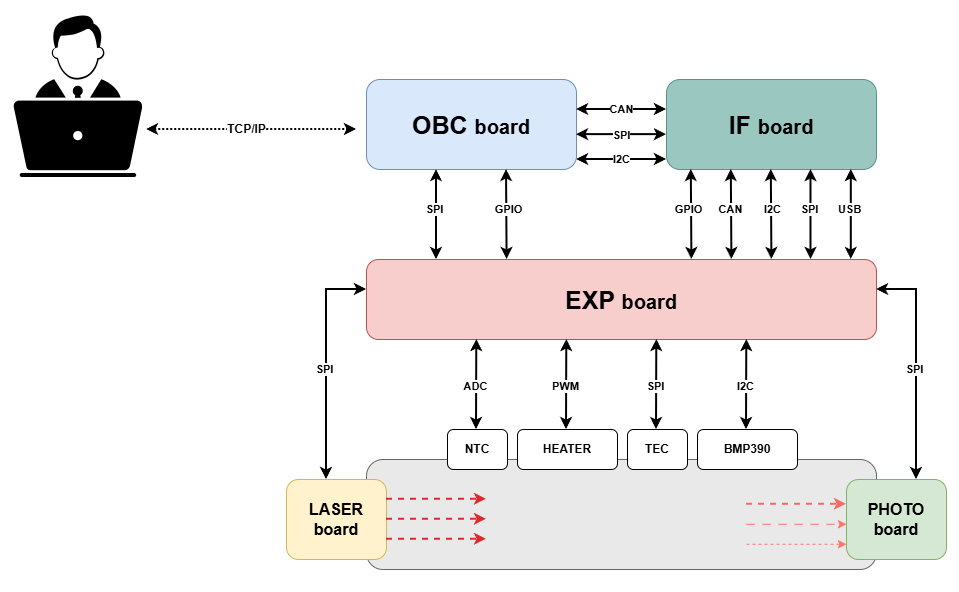
\includegraphics[width=0.85\textwidth]{picture/so-do-tong-quat.png}
    \caption{Sơ đồ khối tổng quát}
    \label{fig:so-do-tong-quat}
\end{figure}

\textbf{Board điều khiển trung tâm (OBC):}
OBC là khối điều phối ở mức hệ thống, tiếp nhận lệnh từ phía người vận hành và phát lệnh tác vụ xuống khối thí nghiệm.
Board này đồng thời thu nhận dữ liệu phản hồi từ EXP, tổng hợp trạng thái toàn hệ và lưu các thông tin quan trọng của phiên thí nghiệm để phục vụ theo dõi và hậu kiểm.
Trong cấu hình triển khai, OBC đóng vai trò \textit{master} của mạng điều khiển nội bộ.

\textbf{Board điều khiển thí nghiệm (EXP):}
EXP là bộ điều khiển cục bộ của tải thí nghiệm.
Khi nhận lệnh từ OBC, EXP thực hiện chu trình thí nghiệm: điều khiển board LASER, thu dữ liệu từ board PHOTO, đọc dữ liệu cảm biến môi trường (như NTC) và điều phối phần tử chấp hành nhiệt (HEATER/TEC).
Sau mỗi chu kỳ đo, EXP chuẩn hóa và đóng gói dữ liệu trước khi gửi ngược lên OBC.

\textbf{Board giao tiếp trung gian (IF):}
IF là tầng \textit{interface}, có nhiệm vụ chuẩn hóa kết nối, tổ chức đường tín hiệu và hỗ trợ mở rộng ngoại vi.
Khối này giúp tách lớp điều khiển chính khỏi các ràng buộc kết nối phần cứng, nhờ đó hệ thống dễ tích hợp thêm module mới, đồng thời giảm độ phức tạp khi thay đổi cấu hình thử nghiệm.

\textbf{Board phát quang (LASER):}
Board LASER tạo nguồn sáng kích thích cho quá trình đo mẫu.
Mạch được thiết kế theo cấu trúc nhiều kênh độc lập, cho phép lựa chọn từng kênh phát theo lệnh điều khiển từ EXP.
Cường độ phát có thể hiệu chỉnh để phù hợp với từng điều kiện thí nghiệm và từng loại mẫu vật.

\textbf{Board thu quang (PHOTO):}
Board PHOTO tiếp nhận tín hiệu ánh sáng sau khi tương tác với mẫu và biến đổi thành tín hiệu điện phục vụ đo lường.
Khối này tích hợp mạch khuếch đại, lọc nhiễu và chuyển đổi ADC để bảo đảm tín hiệu thu có chất lượng tốt trước khi truyền về EXP.
Vị trí các kênh thu được bố trí tương ứng với các kênh phát trên board LASER nhằm bảo đảm tính đồng bộ khi quét mẫu.

\section{Sơ đồ khối chi tiết}
\subsection{Board máy tính điều khiển trung tâm - OBC}
\label{subsec:board-dieu-khien-trung-tam-obc}

Board OBC là trung tâm điều khiển và xử lý dữ liệu của hệ thống, đảm nhiệm vai trò giao tiếp với người vận hành, 
quản lý các tác vụ điều khiển và lưu trữ dữ liệu thí nghiệm. Sơ đồ khối chi tiết của board OBC được trình bày trong Hình \ref{fig:so-do-chi-tiet-obc}.

\begin{figure}[H]
    \centering
    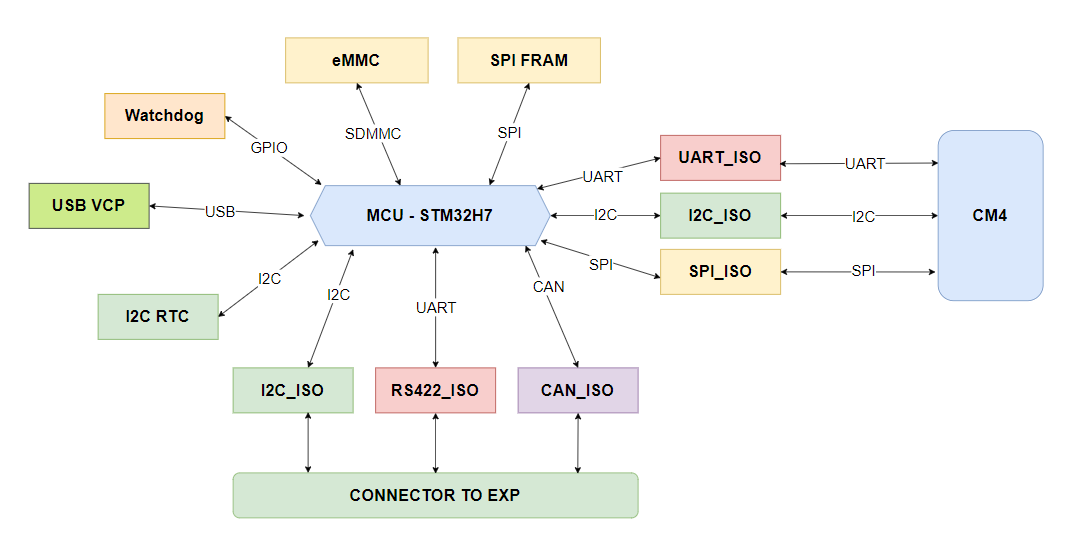
\includegraphics[width=1\textwidth]{picture/OBC.png}
    \caption{Sơ đồ khối chi tiết của board điều khiển OBC}
    \label{fig:so-do-chi-tiet-obc}
\end{figure}

Dựa trên sơ đồ Hình~\ref{fig:so-do-chi-tiet-obc}, chức năng các khối chính của board OBC gồm:
\begin{itemize}
    \item \textbf{Khối MCU -- STM32H7:} là bộ xử lý trung tâm của OBC, thực hiện tiếp nhận lệnh điều khiển, điều phối dữ liệu giữa các board mạch và quản lý luồng vận hành tổng thể.

    \item \textbf{Khối Compute Module 4 (CM4):} đảm nhiệm các tác vụ tầng cao như giao tiếp mạng, quản lý cơ sở dữ liệu, truyền nhận lệnh và chạy các tiến trình giám sát hệ thống.

    \item \textbf{Khối SPI Flash \& SPI FRAM:} cung cấp vùng nhớ lưu tham số, nhật ký vận hành và dữ liệu thí nghiệm cần truy cập nhanh và ổn định.

    \item \textbf{Khối Watchdog:} giám sát trạng thái hoạt động phần mềm; khi phát hiện treo hệ thống sẽ kích hoạt cơ chế reset để bảo đảm tính liên tục vận hành.

    \item \textbf{Khối I2C RTC:} duy trì thời gian thực cho hệ thống, phục vụ đóng dấu thời gian cho dữ liệu đo và các sự kiện vận hành.

    \item \textbf{Khối USB VCP:} cung cấp giao diện USB ảo để kết nối với máy tính, hỗ trợ cấu hình, truyền dữ liệu và debug.

    \item \textbf{Khối giao tiếp cách ly:} gồm \textit{UART ISO}, \textit{SPI ISO}, \textit{GPIO ISO}, \textit{I2C ISO}; có chức năng cách ly điện để bảo vệ khối xử lý trước nhiễu và chênh lệch điện áp từ ngoại vi.
\end{itemize}



\subsection{Board điều khiển thí nghiệm - EXP}
\label{subsec:board-dieu-khien-thi-nghiem-exp}

Board điều khiển thí nghiệm (EXP) là trung tâm xử lý và điều phối hoạt động của thí nghiệm, đóng vai trò cầu nối giữa OBC và các khối chức năng như LASER, PHOTO, 
cảm biến môi trường và phần tử chấp hành nhiệt. Sơ đồ khối chi tiết của board EXP được trình bày trong Hình \ref{fig:so-do-khoi-exp}.

\begin{figure}[H]
    \centering
    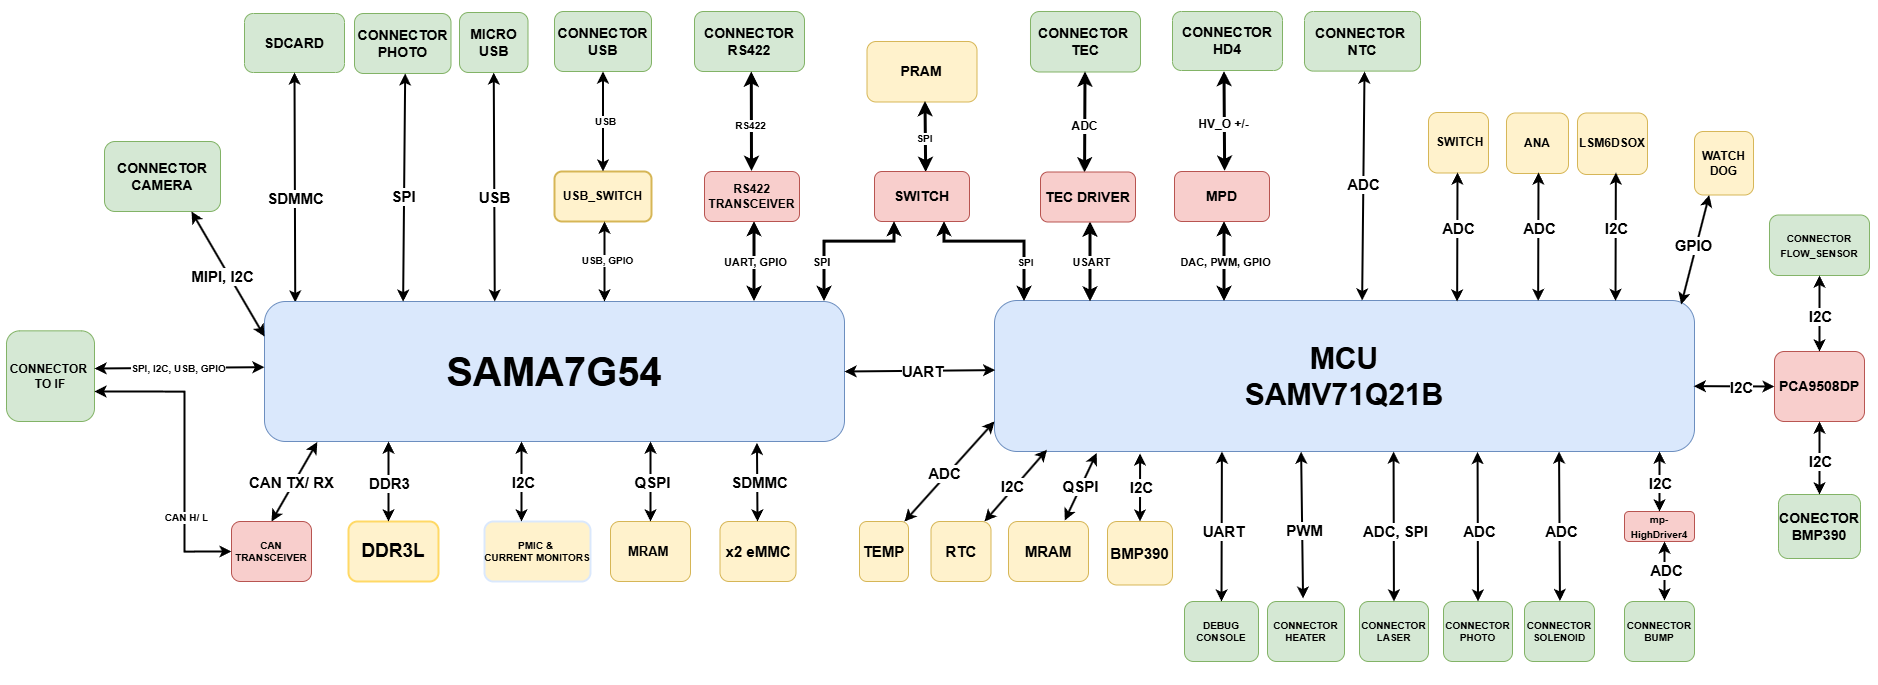
\includegraphics[width=1\textwidth]{picture/exp/so-do-khoi-exp.png}
    \caption{Sơ đồ khối chi tiết board EXP}
    \label{fig:so-do-khoi-exp}
\end{figure}

Dựa trên sơ đồ Hình~\ref{fig:so-do-khoi-exp}, chức năng các khối chính của board EXP gồm:
\begin{itemize}
    \item \textbf{Khối SAMA7G54:} là bộ xử lý chính, thực hiện điều phối tác vụ cấp hệ thống, quản lý truyền thông và trao đổi dữ liệu với MCU qua UART.

    \item \textbf{Khối MCU SAMV71Q21B:} là bộ điều khiển thời gian thực, trực tiếp đọc tín hiệu cảm biến và phát lệnh điều khiển tới các tải chấp hành.

    \item \textbf{Khối DDR3L:} bộ nhớ làm việc tốc độ cao cho SAMA7G54 trong các tác vụ xử lý dữ liệu.

    \item \textbf{Khối MRAM:} bộ nhớ không mất dữ liệu dùng lưu tham số/cấu hình cần giữ lại sau khi mất nguồn.

    \item \textbf{Khối x2 eMMC:} bộ nhớ lưu trữ dung lượng lớn cho chương trình, dữ liệu hệ thống và nhật ký vận hành.

    \item \textbf{Khối PMIC \& current monitors:} cấp nguồn cho các rail điện áp và giám sát dòng tiêu thụ của board.

    \item \textbf{Khối SDCARD:} giao tiếp SDMMC để mở rộng lưu trữ và thuận tiện cho nạp/thu hồi dữ liệu.

    \item \textbf{Khối MICRO USB:} giao tiếp USB phục vụ nạp chương trình, cấu hình hoặc chẩn đoán hệ thống.

    \item \textbf{Khối USB\_SWITCH:} chuyển mạch đường USB theo tín hiệu điều khiển từ SAMA7G54 để chọn tuyến kết nối phù hợp.

    \item \textbf{Khối RS422 TRANSCEIVER:} chuyển mức tín hiệu UART sang RS422, tăng độ bền nhiễu và khoảng cách truyền.

    \item \textbf{Khối CAN TRANSCEIVER:} giao tiếp CAN TX/RX (CAN H/L) để kết nối bus công nghiệp với các thiết bị ngoài.

    \item \textbf{Khối TEC DRIVER:} mạch công suất điều khiển phần tử TEC theo lệnh từ MCU.

    \item \textbf{Khối MPD:} mạch điều khiển/điều áp cao áp (HV\_O +/-) theo DAC/PWM/GPIO từ MCU.

    \item \textbf{Khối mp-HighDriver4:} mạch driver công suất điều khiển tải ngoài (ví dụ cụm bơm) theo tín hiệu ADC/I2C liên quan.

    \item \textbf{Khối TEMP:} kênh đo nhiệt độ đưa về MCU qua ADC để giám sát trạng thái nhiệt.

    \item \textbf{Khối RTC:} đồng hồ thời gian thực, cung cấp mốc thời gian ổn định cho ghi log và điều khiển theo lịch.

    \item \textbf{Khối MRAM 4bits:} vùng nhớ phụ giao tiếp QSPI cho lưu trạng thái nhanh của MCU.

    \item \textbf{Khối PRAM:} bộ nhớ phụ giao tiếp SPI, dùng cho lưu tham số và trao đổi dữ liệu cục bộ.

    \item \textbf{Khối BMP390:} cảm biến áp suất/độ cao kết nối I2C, cung cấp dữ liệu môi trường cho điều khiển.

    \item \textbf{Khối ANA:} đầu vào tín hiệu analog đưa về MCU qua ADC để đo các đại lượng tương tự.

    \item \textbf{Khối LSM6DSOX:} cảm biến IMU (gia tốc - con quay) giao tiếp I2C phục vụ giám sát dao động/chuyển động.

    \item \textbf{Khối WATCHDOG:} phần cứng giám sát hoạt động MCU, tự động can thiệp khi hệ thống treo hoặc mất đáp ứng.

    \item \textbf{Khối PCA9508DP:} mở rộng I/O qua I2C, làm cầu nối điều khiển/đọc thêm các kênh ngoại vi.

    \item \textbf{Khối DEBUG CONSOLE:} cổng UART phục vụ debug, theo dõi log và chẩn đoán khi phát triển.

    \item \textbf{Khối SWITCH:} các công tắc chuyển mạch nội bộ (SPI/ADC) dùng để chọn đường tín hiệu, cấu hình tuyến đo và phân phối tín hiệu điều khiển.

    \item \textbf{Khối connector CAMERA:} kết nối camera qua giao thức \textit{MIPI} (dữ liệu ảnh) và \textit{I2C} (cấu hình).

    \item \textbf{Khối connector TO IF:} kết nối sang board IF qua các đường \textit{SPI}, \textit{I2C}, \textit{USB} và \textit{GPIO}.

    \item \textbf{Khối connector MATO:} giao tiếp ngoại vi theo chuẩn \textit{SPI}.

    \item \textbf{Khối connector MICRO USB:} giao tiếp theo chuẩn \textit{USB}.

    \item \textbf{Khối connector USB:} giao tiếp \textit{USB} thông qua khối \textit{USB\_SWITCH}.

    \item \textbf{Khối connector RS422:} giao tiếp truyền thông theo chuẩn \textit{RS422}.

    \item \textbf{Khối connector TEC:} nhận/tương tác tín hiệu điều khiển - đo theo đường \textit{ADC} của nhánh TEC.

    \item \textbf{Khối connector HD4:} kết nối nhánh tải HD4 theo đường công suất \textit{HV\_O +/-}.

    \item \textbf{Khối connector NTC:} đưa tín hiệu nhiệt độ về MCU qua kênh \textit{ADC}.

    \item \textbf{Khối connector FLOW\_SENSOR:} kết nối cảm biến lưu lượng qua bus \textit{I2C}.

    \item \textbf{Khối connector BMP390:} kết nối cảm biến BMP390 qua bus \textit{I2C}.

    \item \textbf{Khối connector HEATER:} nhận tín hiệu điều khiển công suất theo \textit{PWM}.

    \item \textbf{Khối connector LASER:} kết nối điều khiển/giám sát qua các đường \textit{ADC} và \textit{SPI}.

    \item \textbf{Khối connector PHOTO:} nhận tín hiệu đo quang về MCU qua kênh \textit{ADC}.

    \item \textbf{Khối connector SOLENOID:} điều khiển và giám sát tải solenoid qua đường \textit{ADC}.

    \item \textbf{Khối connector BUMP:} kết nối nhánh bơm qua tín hiệu điều khiển/giám sát \textit{ADC}.
\end{itemize}

\subsection{Board giao tiếp - IF}
\label{subsec:board-giao-tiep-if}
\begin{figure}[H]
    \centering
    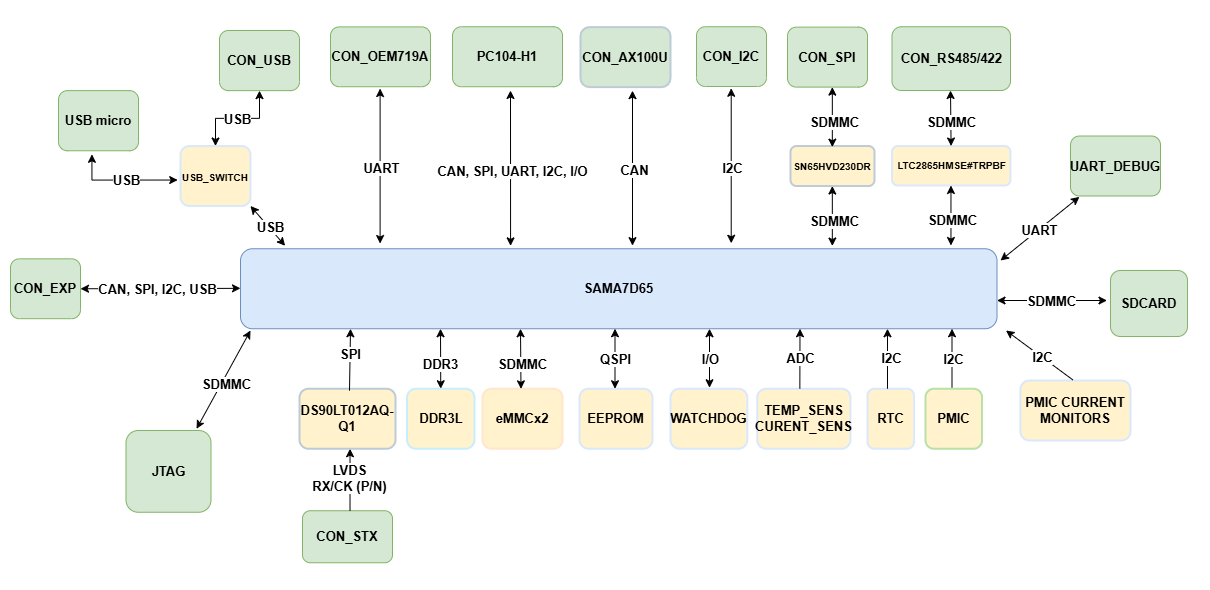
\includegraphics[width=1\textwidth]{picture/if/so-do-khoi-if.png}
    \caption{Sơ đồ khối chi tiết board IF}
    \label{fig:so-do-khoi-if}
\end{figure}

Board IF giữ vai trò là nơi giao tiếp hệ thống thí nghiệm với các chức năng bên ngoài, đồng thời hỗ trợ nhiều chuẩn giao tiếp công nghiệp như RS422, LVDS. Sơ đồ khối chi tiết của board IF được trình bày trong Hình \ref{fig:so-do-khoi-if}.

Dựa trên sơ đồ Hình~\ref{fig:so-do-khoi-if}, chức năng các khối chính của board IF gồm:
\begin{itemize}
    \item \textbf{Khối SAMA7D65:} là bộ xử lý trung tâm của IF, đảm nhiệm điều phối toàn bộ luồng giao tiếp, quản lý dữ liệu giữa các cổng kết nối và điều khiển các ngoại vi đi kèm.

    \item \textbf{Khối CON\_EXP:} là cổng kết nối chính với board EXP, trao đổi các đường \textit{CAN}, \textit{SPI}, \textit{I2C} và \textit{USB} để đồng bộ lệnh và dữ liệu liên board.

    \item \textbf{Khối USB micro -- USB\_SWITCH -- CON\_USB:} tạo tuyến giao tiếp USB linh hoạt, cho phép chuyển mạch đường USB giữa cổng vào và cổng ra theo cấu hình vận hành.

    \item \textbf{Nhóm cổng mở rộng ngoại vi:} gồm \textit{CON\_OEM719A}, \textit{PC104-H1}, \textit{CON\_AX100U}, \textit{CON\_I2C}, \textit{CON\_SPI}, \textit{CON\_RS485/422}; cung cấp các chuẩn giao tiếp \textit{UART/CAN/SPI/I2C/IO} để tích hợp thiết bị ngoài.

    \item \textbf{Khối SN65HVD230DR và LTC2865HMSE\#TRPBF:} là các transceiver truyền thông, thực hiện chuyển mức và tăng khả năng chống nhiễu cho các đường truyền công nghiệp.

    \item \textbf{Khối SDCARD:} cung cấp lưu trữ rời qua giao tiếp \textit{SDMMC}, phục vụ ghi log, lưu cấu hình và trích xuất dữ liệu hệ thống.

    \item \textbf{Khối DDR3L và eMMCx2:} cung cấp bộ nhớ làm việc tốc độ cao và bộ nhớ lưu trữ không mất dữ liệu cho tác vụ xử lý và vận hành của IF.

    \item \textbf{Khối EEPROM:} lưu các tham số cấu hình và thông tin hiệu chỉnh cần giữ bền vững trong quá trình vận hành.

    \item \textbf{Khối WATCHDOG:} giám sát trạng thái xử lý của bộ điều khiển; khi phát hiện bất thường sẽ kích hoạt cơ chế phục hồi nhằm tăng độ tin cậy hệ thống.

    \item \textbf{Khối TEMP\_SENS/CURENT\_SENS, PMIC và PMIC CURRENT MONITORS:} đo nhiệt độ, dòng tiêu thụ và quản lý nguồn, hỗ trợ giám sát hệ thống theo thời gian thực.

    \item \textbf{Khối RTC, UART\_DEBUG, JTAG và DS90LT012AQ-Q1/CON\_STX:} hỗ trợ đóng dấu thời gian, debug -- nạp chương trình và truyền/nhận tín hiệu chuyên dụng phục vụ kiểm thử, khai thác hệ thống.
\end{itemize}

\subsection{Board phát năng lượng ánh sáng - LASER}
\label{subsec:board-phat-laser}
\begin{figure}[H]
    \centering
    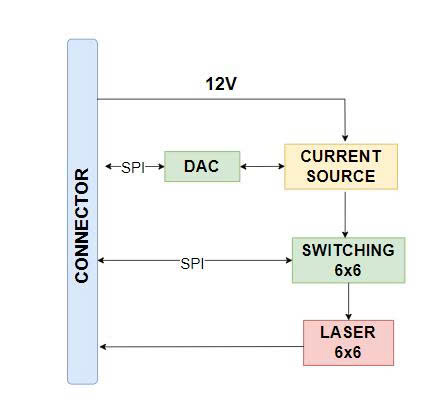
\includegraphics[width=0.6\textwidth]{picture/laser/so-do-khoi-laser.jpg}
    \caption{Sơ đồ khối chi tiết board LASER}
    \label{fig:so-do-khoi-laser}
\end{figure}

Board phát năng lượng ánh sáng (LASER) đảm nhiệm vai trò tạo tín hiệu kích thích quang theo kênh, cho phép lựa chọn vị trí phát và điều chỉnh mức kích tương ứng với từng cấu hình thí nghiệm.
Sơ đồ khối chi tiết của board LASER được trình bày trong Hình \ref{fig:so-do-khoi-laser}.

Dựa trên sơ đồ Hình~\ref{fig:so-do-khoi-laser}, chức năng các khối chính của board LASER gồm:
\begin{itemize}
    \item \textbf{Khối CONNECTOR:} là giao diện kết nối giữa board LASER với board điều khiển, nhận nguồn cấp \(12V\), nhận lệnh điều khiển và trả về tín hiệu trạng thái theo bus \textit{SPI}.

    \item \textbf{Khối DAC:} chuyển đổi lệnh số từ bộ điều khiển thành mức điện áp tham chiếu tương tự, làm đầu vào đặt mức cho mạch phát dòng.

    \item \textbf{Khối CURRENT SOURCE:} tạo dòng kích ổn định cho nhánh phát quang theo mức tham chiếu từ DAC, giúp duy trì cường độ phát theo giá trị đặt.

    \item \textbf{Khối SWITCHING 6x6:} thực hiện ma trận chọn kênh phát, định tuyến dòng kích từ mạch nguồn dòng đến từng phần tử laser theo lệnh điều khiển.

    \item \textbf{Khối LASER 6x6:} là ma trận phần tử phát quang đầu ra, phát ánh sáng theo kênh đã được chọn để kích thích mẫu trong buồng đo.
\end{itemize}


\subsection{Board thu năng lượng ánh sáng - PHOTO}
\label{subsec:board-thu-photo}
\begin{figure}[H]
    \centering
    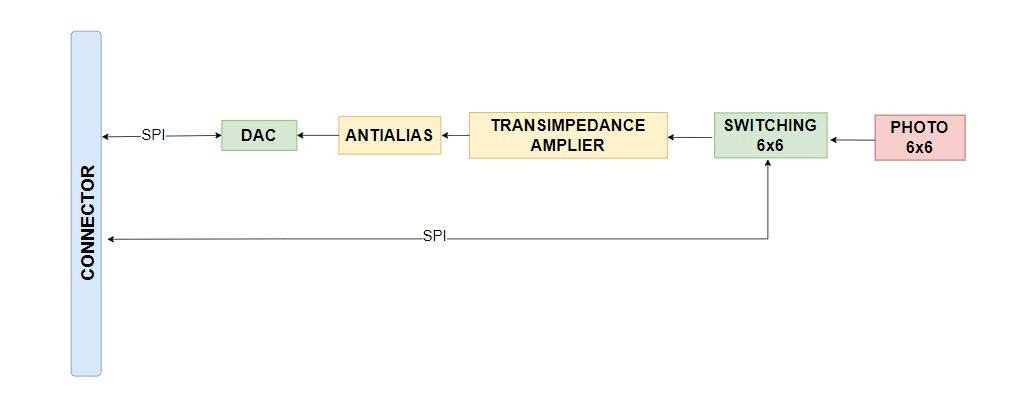
\includegraphics[width=1\textwidth]{picture/photo/so-do-khoi-photo.jpg}
    \caption{Sơ đồ khối chi tiết board PHOTO}
    \label{fig:so-do-khoi-photo}
\end{figure}

Board thu năng lượng ánh sáng (PHOTO) đảm nhiệm vai trò thu tín hiệu quang sau tương tác với mẫu, khuếch đại - lọc tín hiệu và đưa về tín hiệu phù hợp để số hóa.
Sơ đồ khối chi tiết của board PHOTO được trình bày trong Hình \ref{fig:so-do-khoi-photo}.

Dựa trên sơ đồ Hình~\ref{fig:so-do-khoi-photo}, chức năng các khối chính của board PHOTO gồm:
\begin{itemize}
    \item \textbf{Khối CONNECTOR:} là giao diện kết nối với board điều khiển, trao đổi tín hiệu điều khiển/thu thập dữ liệu qua bus \textit{SPI}.

    \item \textbf{Khối PHOTO 6x6:} là ma trận phần tử thu quang, tiếp nhận tín hiệu ánh sáng từ hệ quang và tạo tín hiệu dòng tương ứng cường độ thu được.

    \item \textbf{Khối SWITCHING 6x6:} thực hiện chọn kênh thu trong ma trận PHOTO, định tuyến tín hiệu từ phần tử thu được chọn sang chuỗi xử lý tương tự.

    \item \textbf{Khối TRANSIMPEDANCE AMPLIFIER:} chuyển đổi dòng quang điện sang điện áp và khuếch đại tín hiệu mức nhỏ từ cảm biến quang.

    \item \textbf{Khối ANTIALIAS:} lọc giới hạn băng thông tín hiệu trước khi số hóa, giảm nhiễu cao tần và hạn chế méo aliasing trong quá trình lấy mẫu.

    \item \textbf{Khối DAC:} tạo mức tham chiếu/bù offset cho chuỗi xử lý tương tự theo cấu hình đo, giúp tối ưu dải đo tại ngõ vào bộ chuyển đổi số.
\end{itemize}

\section{Sơ đồ nguyên lí chi tiết}

\subsection{Board máy tính điều khiển trung tâm - OBC}
\label{subsec:sche-board-dieu-khien-trung-tam-obc}

\subsection{Board điều khiển thí nghiệm - EXP}
\label{subsec:sche-board-dieu-khien-thi-nghiem-exp}

\begin{figure}[H]
    \centering
    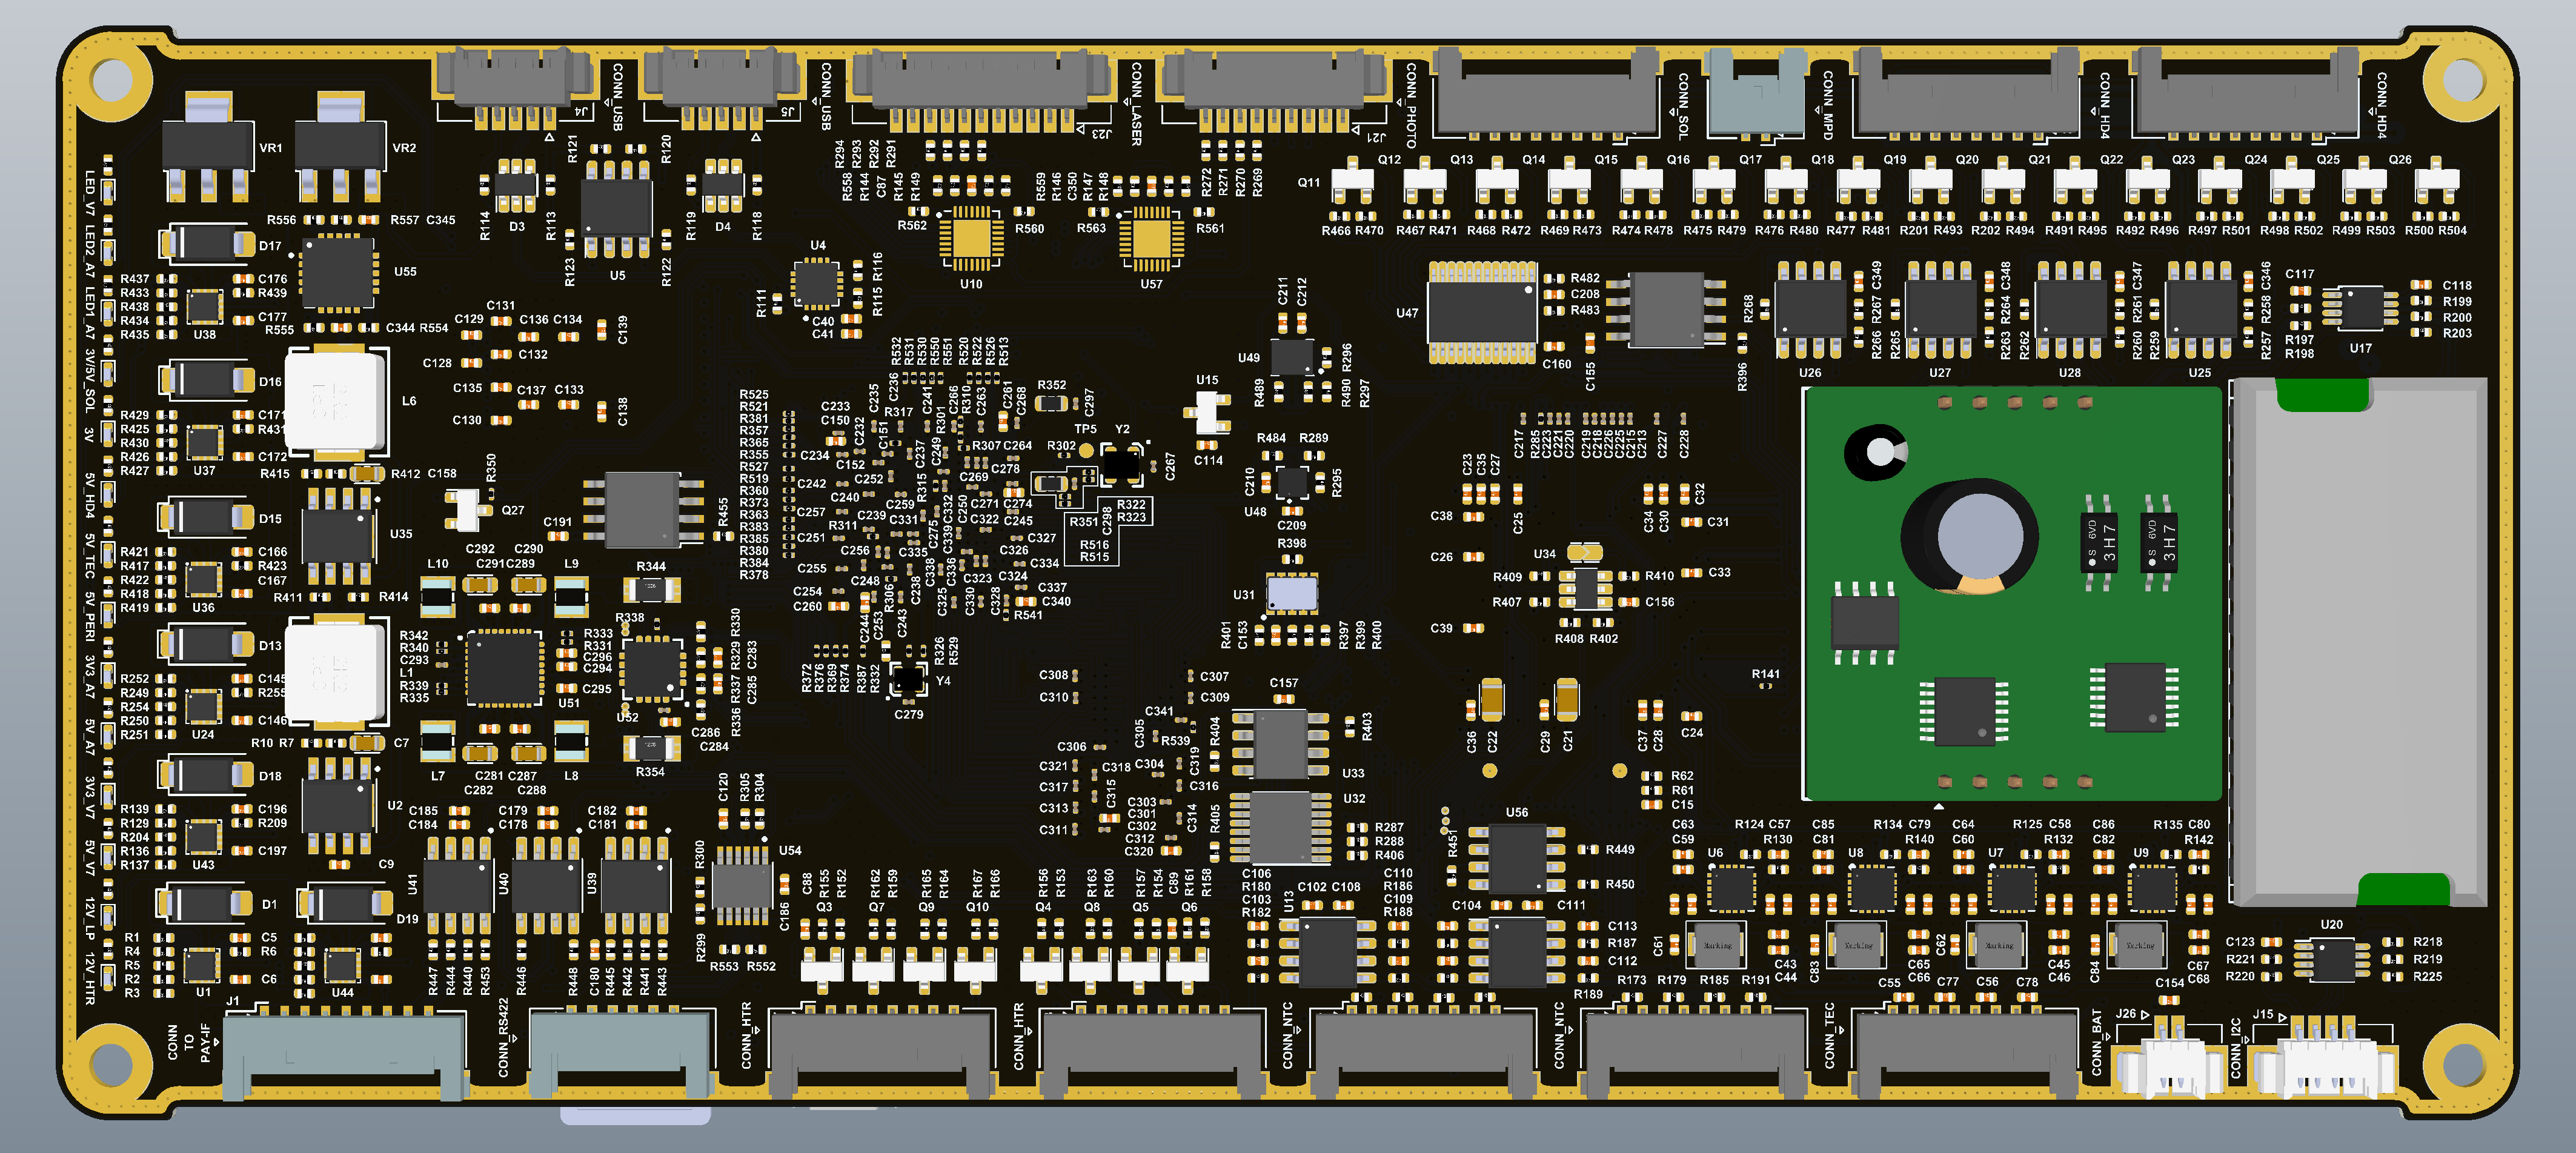
\includegraphics[width=1\textwidth]{picture/exp/BEE_1012 PAY-EXP V100.png}
    
    Mặt trên
    
    \vspace{0.5em}
    
    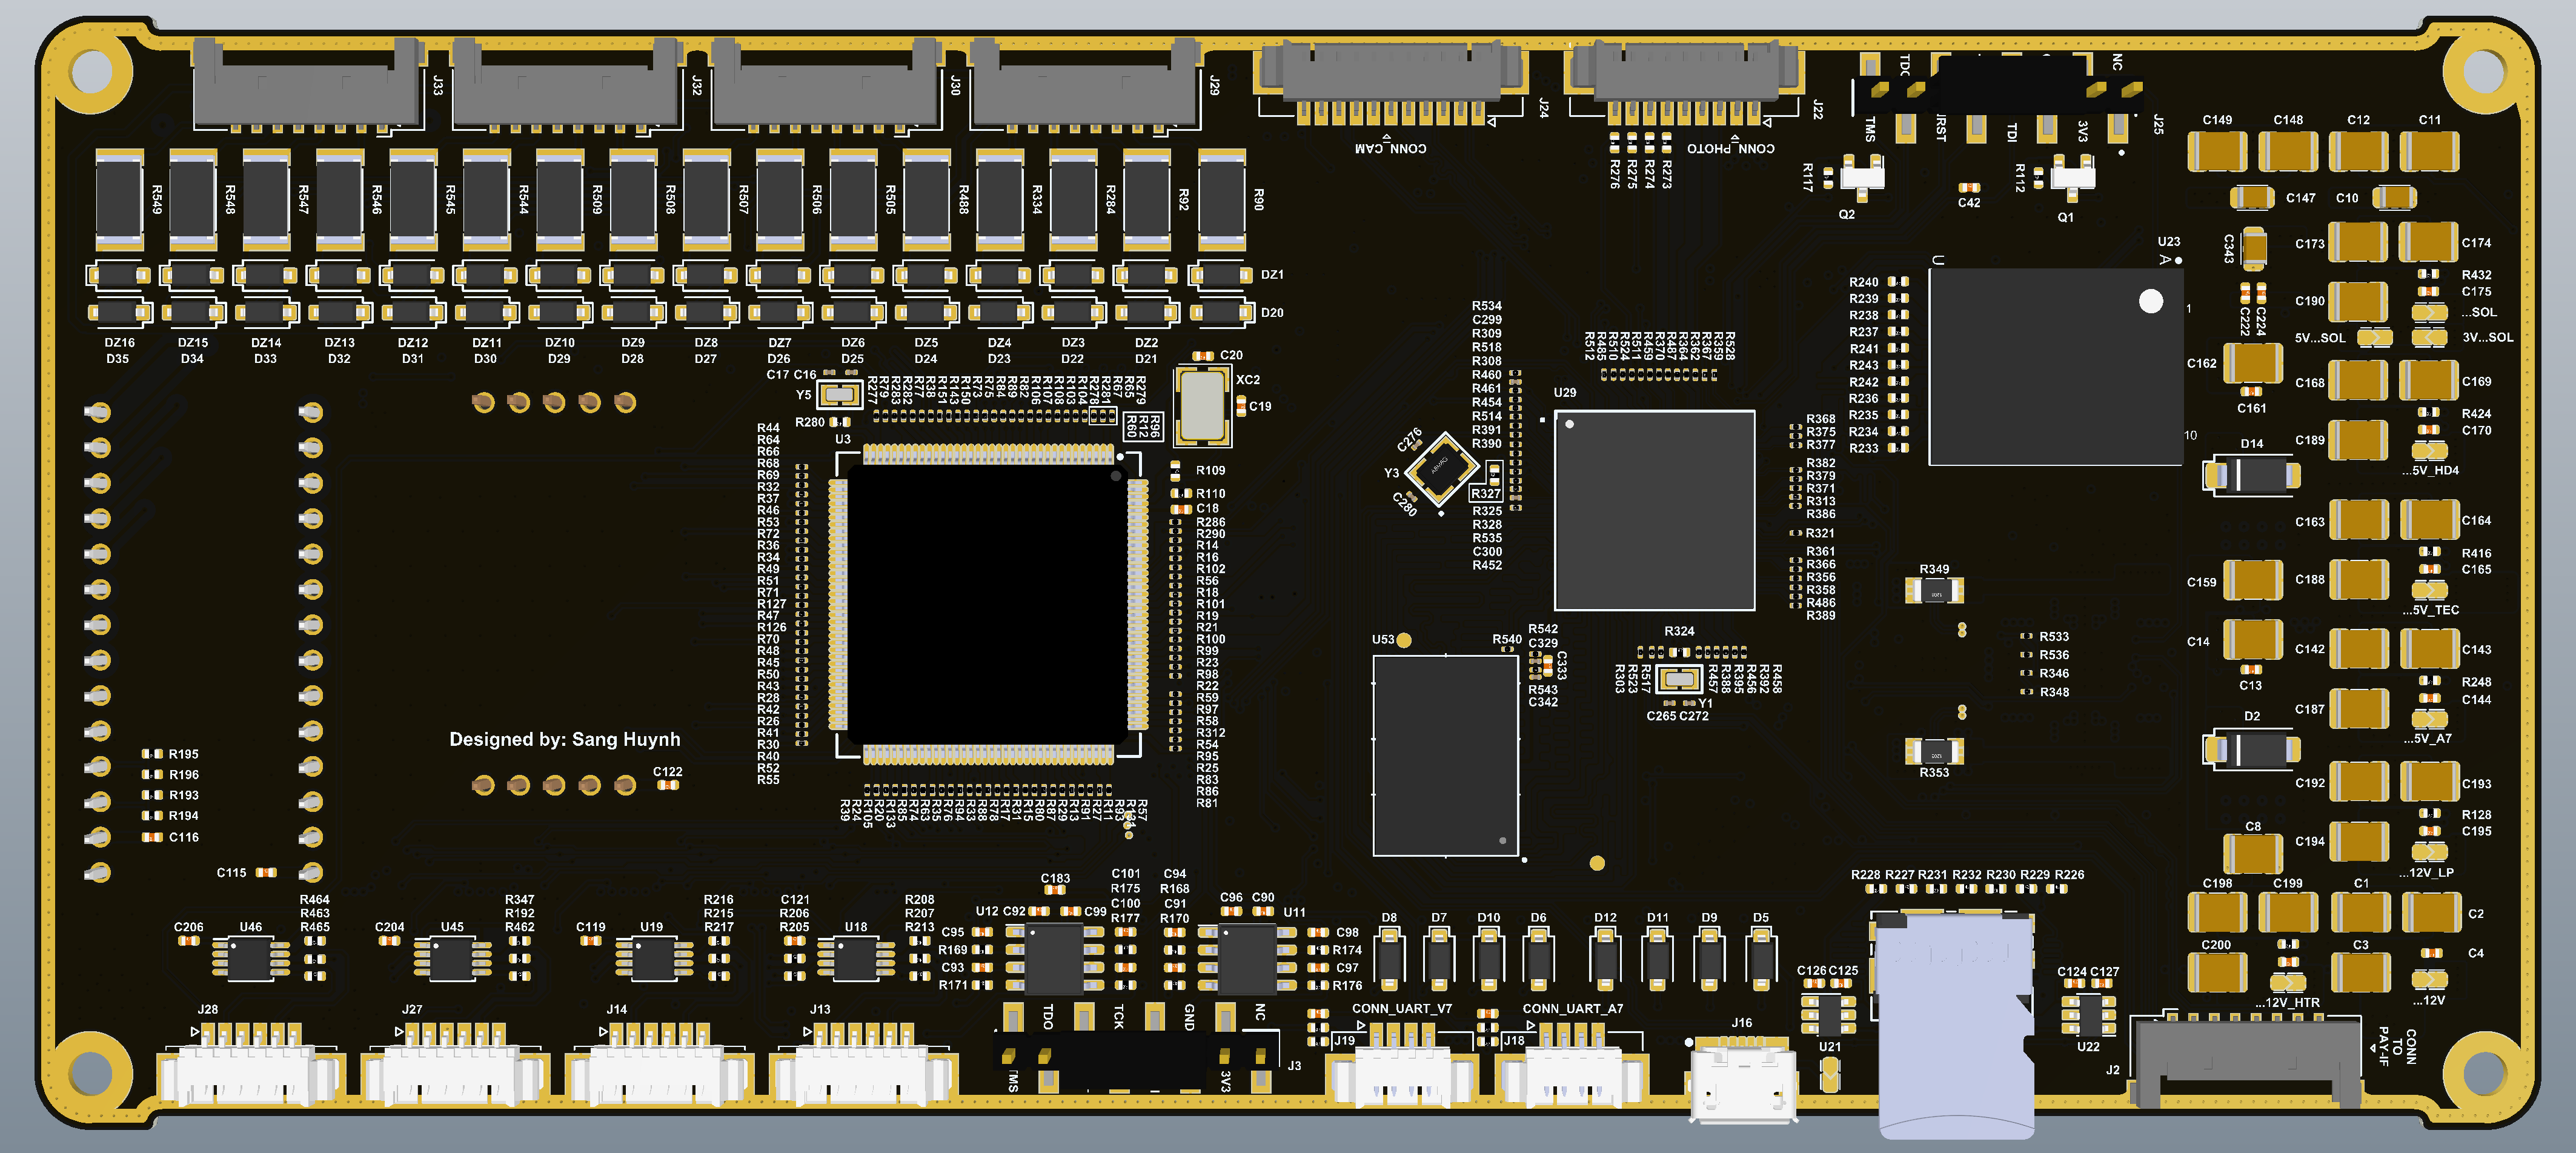
\includegraphics[width=1\textwidth]{picture/exp/BEE_1012 PAY-EXP V100-bot.png}
    
    Mặt dưới
    \caption{PCB board EXP}
    \label{fig:exp-pcb-board}
\end{figure}

Phần này trình bày chi tiết các sơ đồ nguyên lý của board EXP theo từng khối chức năng. Toàn bộ hình schematic được lấy từ thư mục picture/exp, ngoại trừ hình so-do-khoi-exp.png (đã trình bày ở phần sơ đồ khối).

\begin{figure}[H]
    \centering
    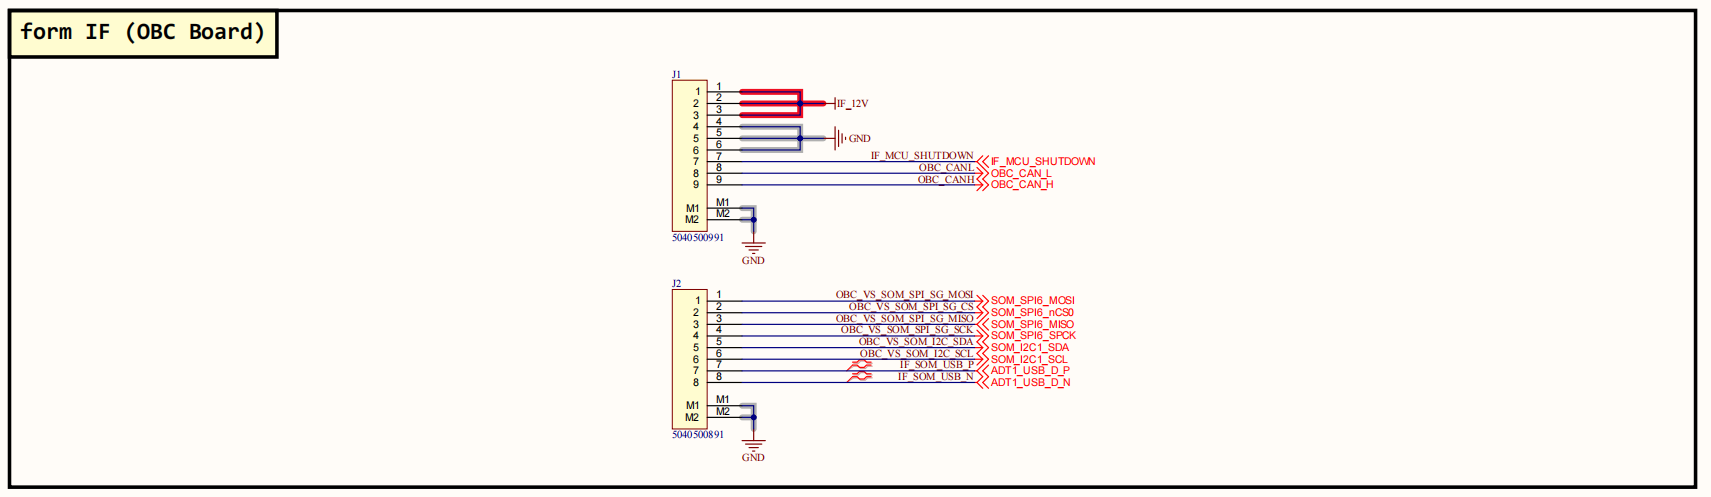
\includegraphics[width=1\textwidth]{picture/exp/connector-if.png}
    \caption{Connector kết nối với board IF}
    \label{fig:exp-sche-connector-if}
\end{figure}
Connector này kết nối với board IF thông qua các tín hiệu CAN, SPI, I2C, USB, tín hiệu IO để bật nguồn cho board IF và lấy nguồn chính 12V thông qua bus 12V chung từ board IF.

\begin{figure}[H]
    \centering
    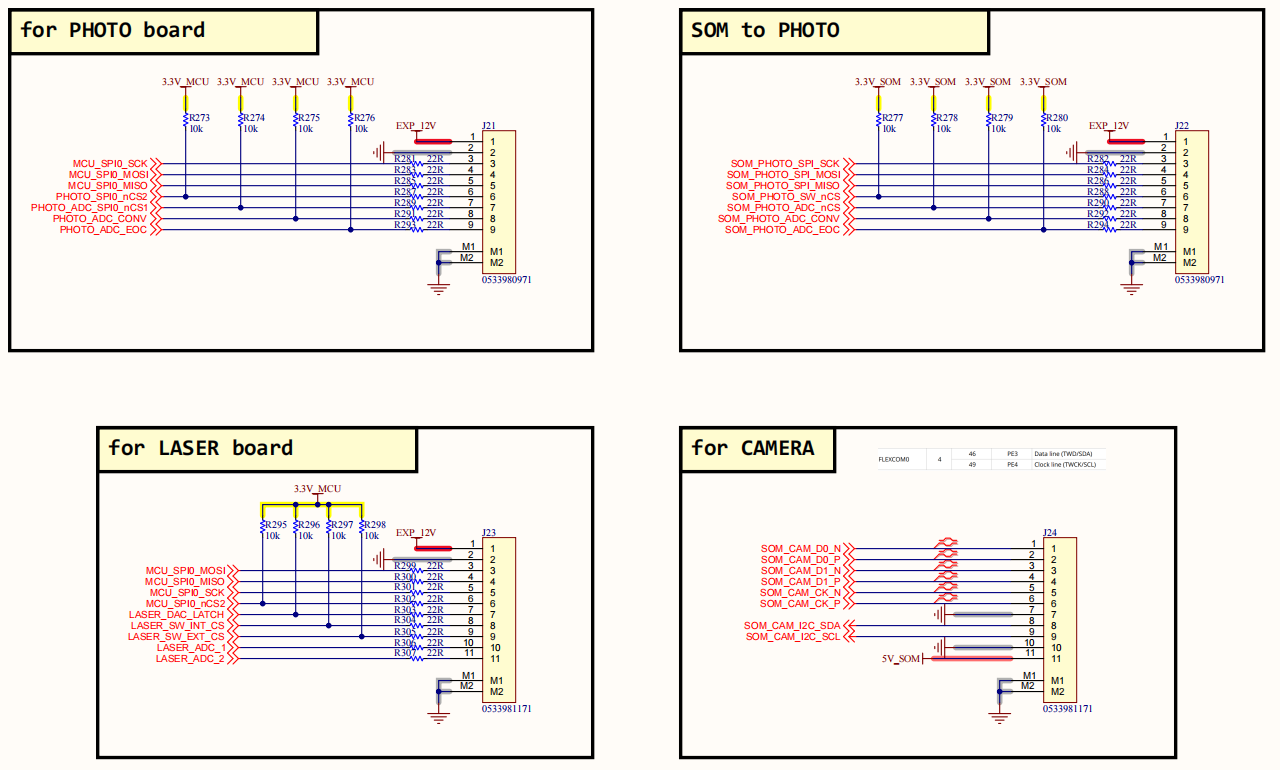
\includegraphics[width=1\textwidth]{picture/exp/connector-thi-nghiem.png}
    \caption{Nhóm connector thí nghiệm}
    \label{fig:exp-sche-connector-thi-nghiem}
\end{figure}
Đây là nhóm đầu nối chính đưa tín hiệu điều khiển/đo lường ra hệ thí nghiệm, đóng vai trò giao diện vật lý giữa EXP và tải ngoài. Connector kết nối đến board PHOTO và LASER thông qua tín hiệu ADC và SPI trên core MCU của EXP, bên cạnh đó core MPU cũng kết nối đến board PHOTO thông qua SPI. Một connector camera với giao tiếp MIPI và I2C để thu thập hình ảnh thí nghiệm.

\begin{figure}[H]
    \centering
    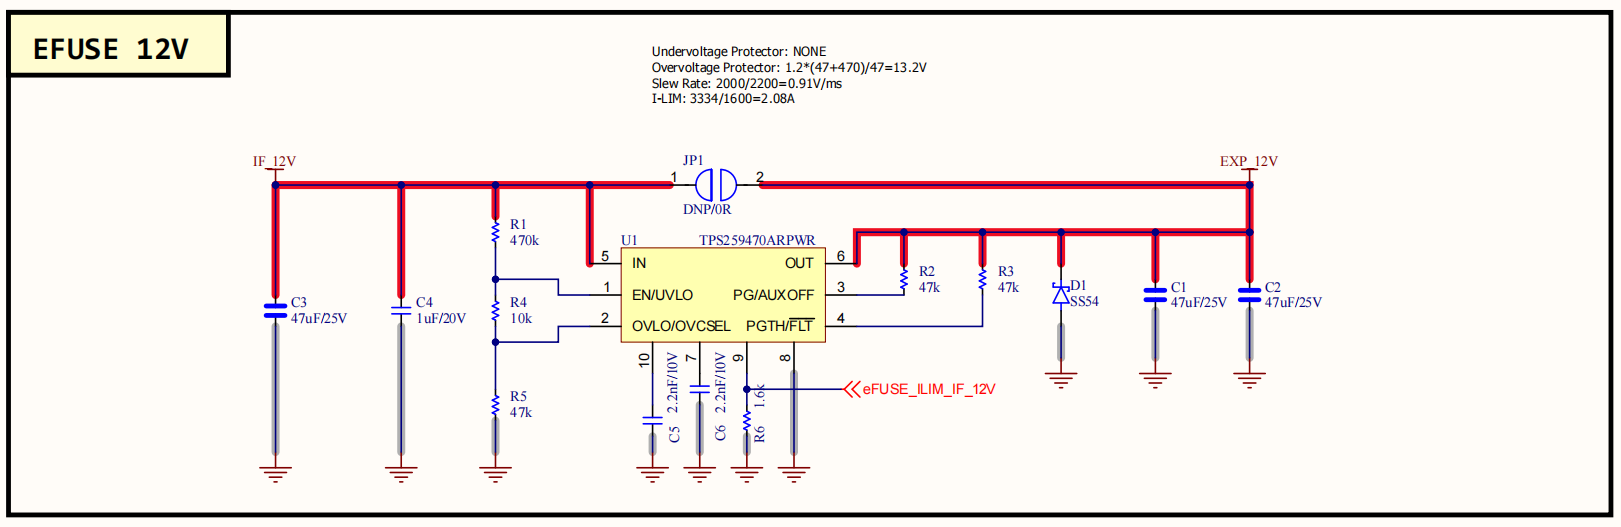
\includegraphics[width=0.48\textwidth]{picture/exp/efuse-12v-if.png}\hfill
    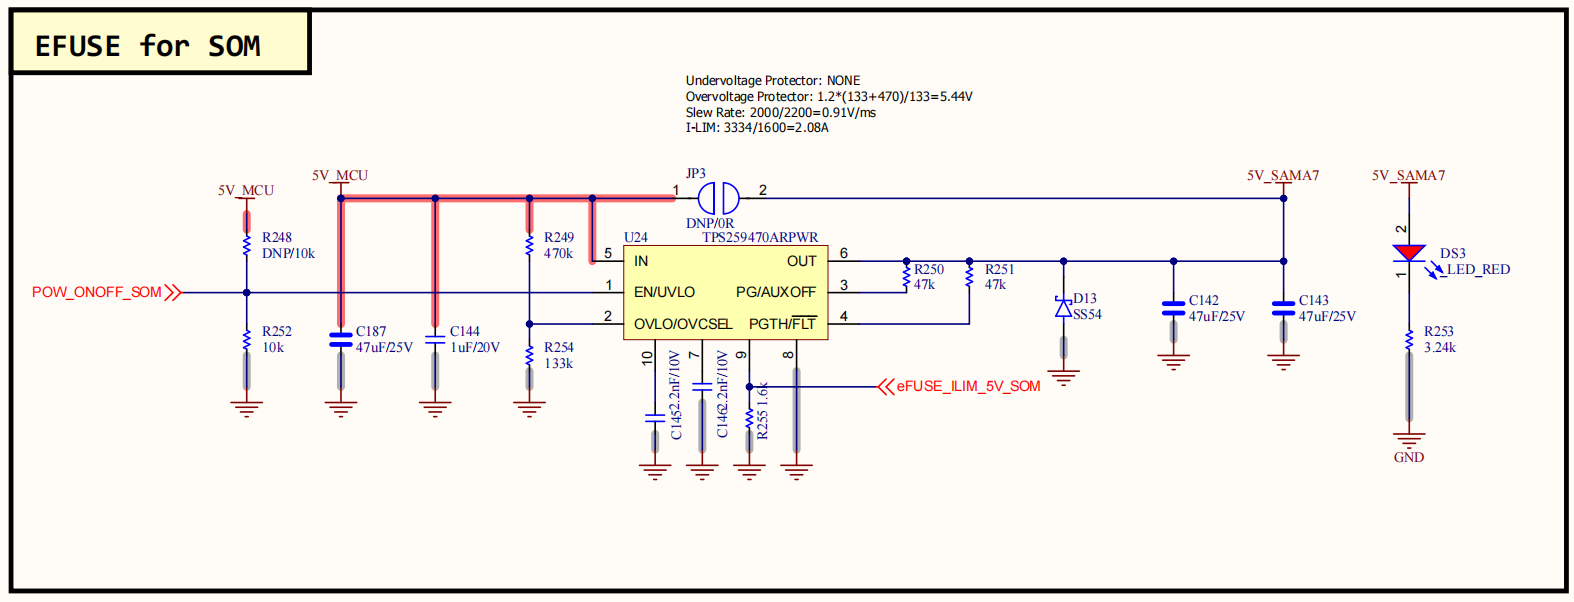
\includegraphics[width=0.48\textwidth]{picture/exp/efuse-5vmcu-5vsam.png}\\[0.8em]

    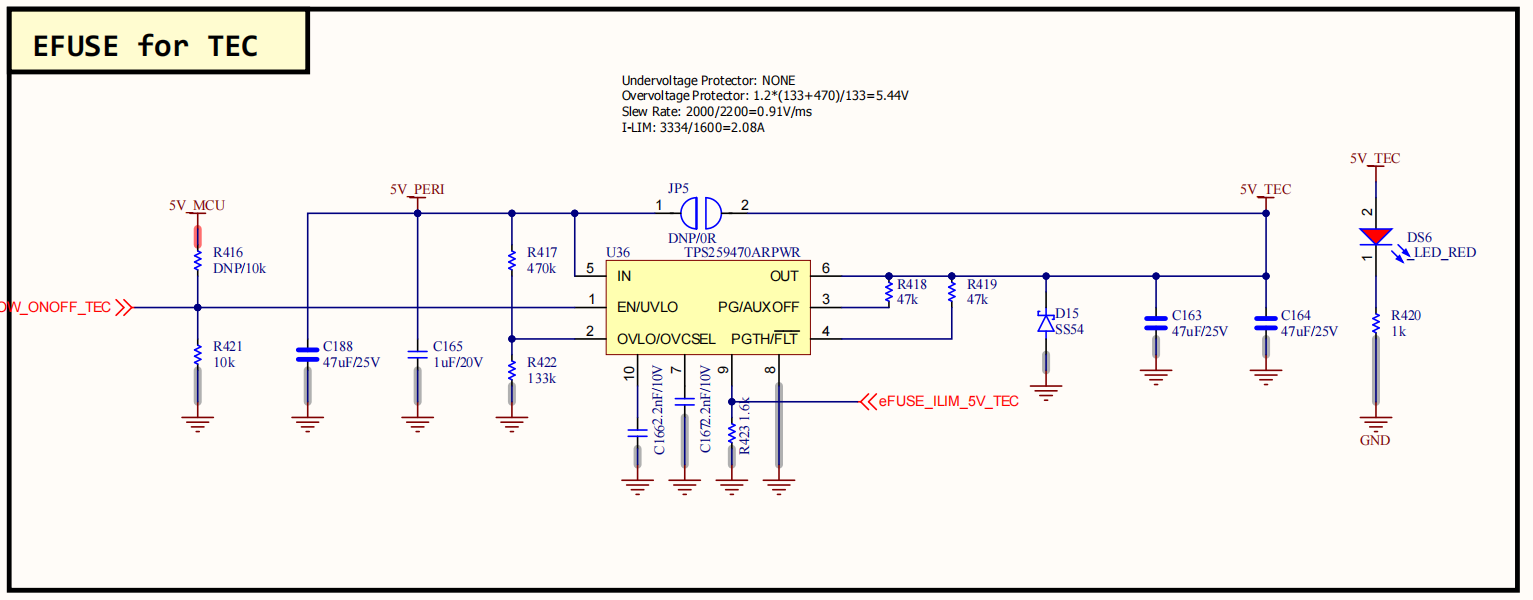
\includegraphics[width=0.48\textwidth]{picture/exp/efuse-5vmcu-5vtec.png}\hfill
    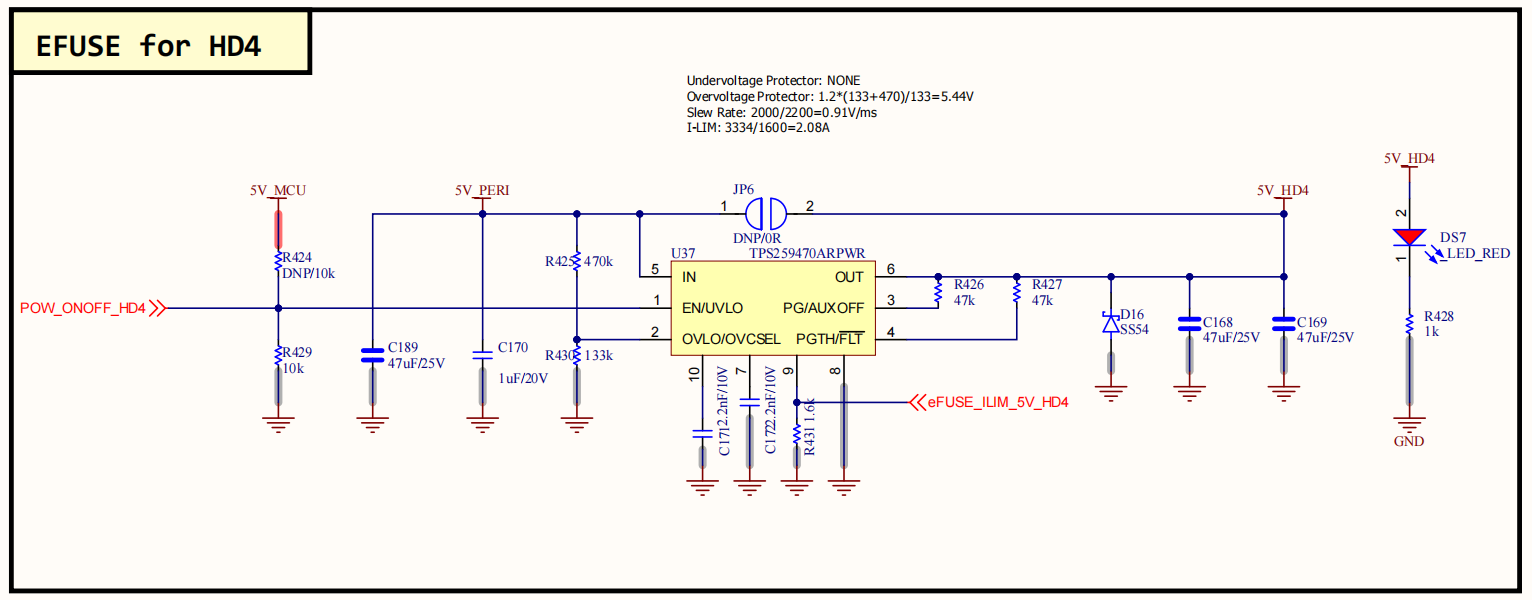
\includegraphics[width=0.48\textwidth]{picture/exp/efuse-5vmcu-5vhd4.png}\\[0.8em]

    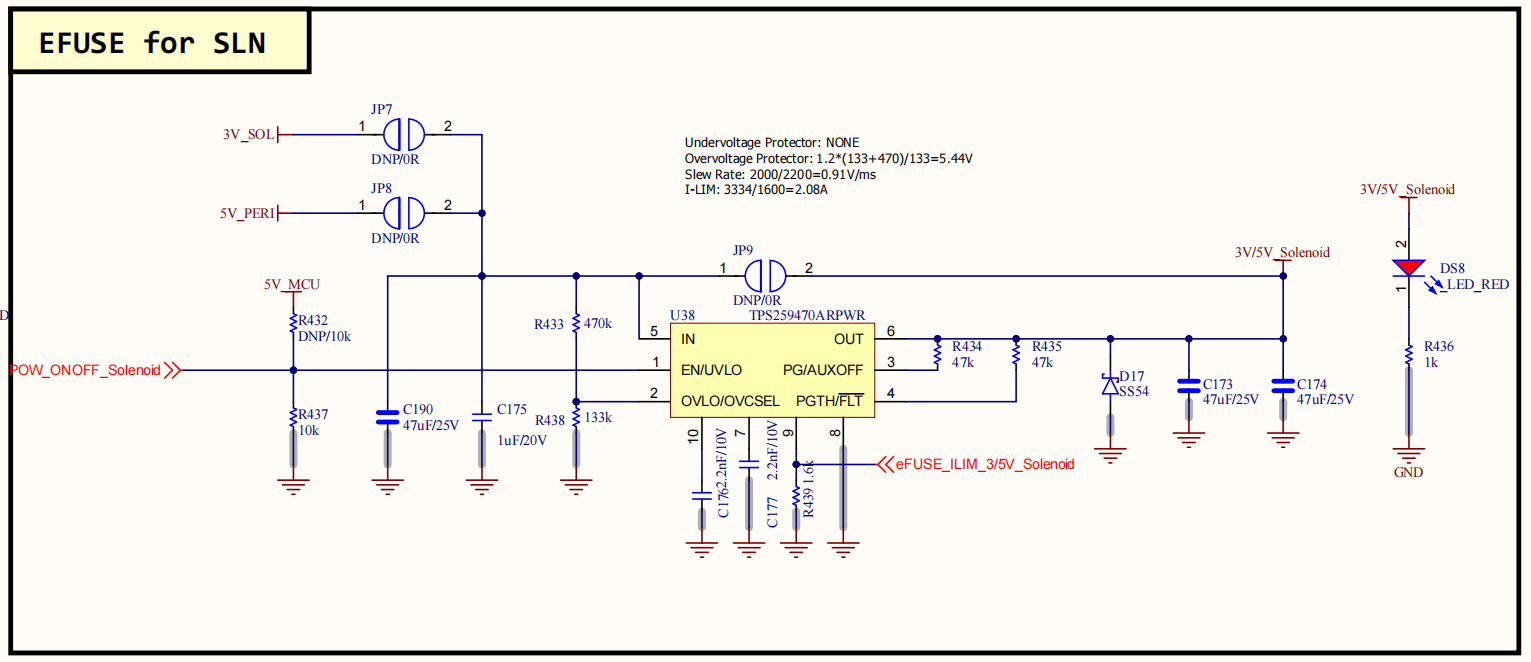
\includegraphics[width=0.48\textwidth]{picture/exp/efuse-solenoid.png}\hfill
    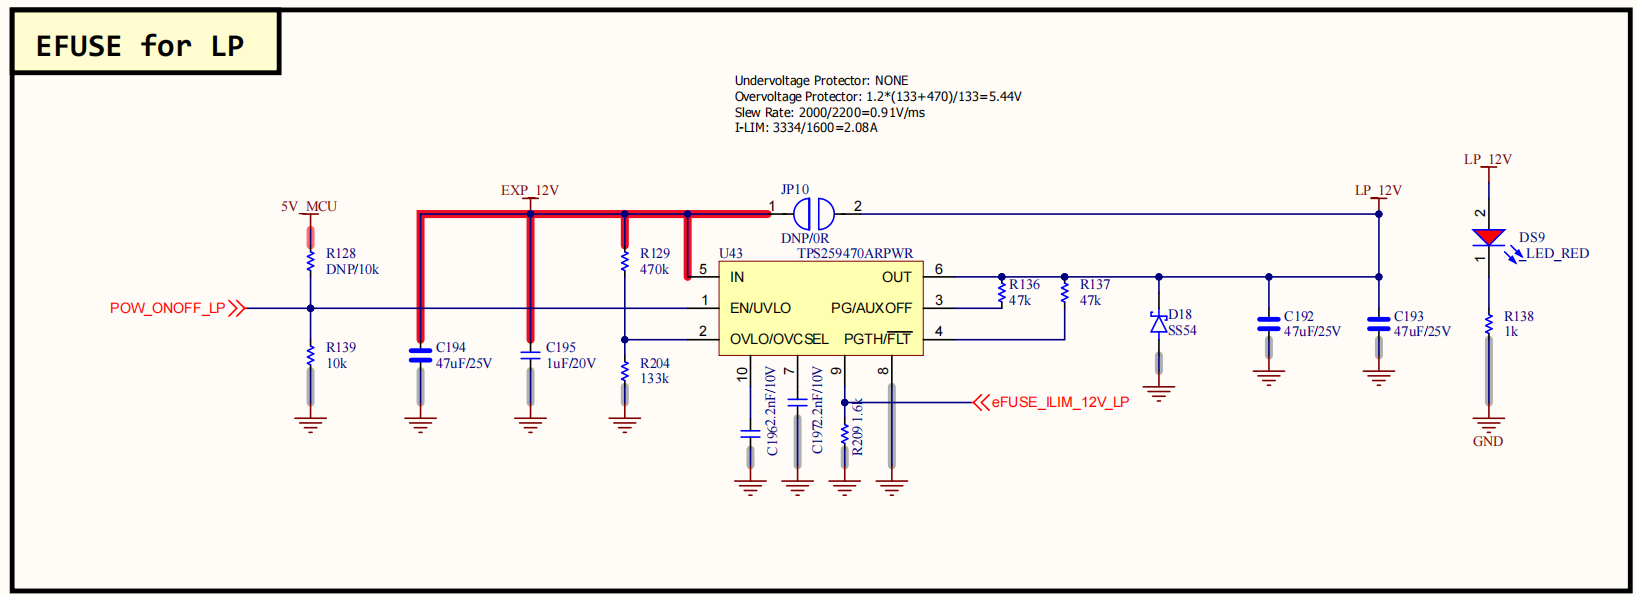
\includegraphics[width=0.48\textwidth]{picture/exp/efuse-12vexp-12vlp.png}\\[0.8em]

    \makebox[\textwidth][c]{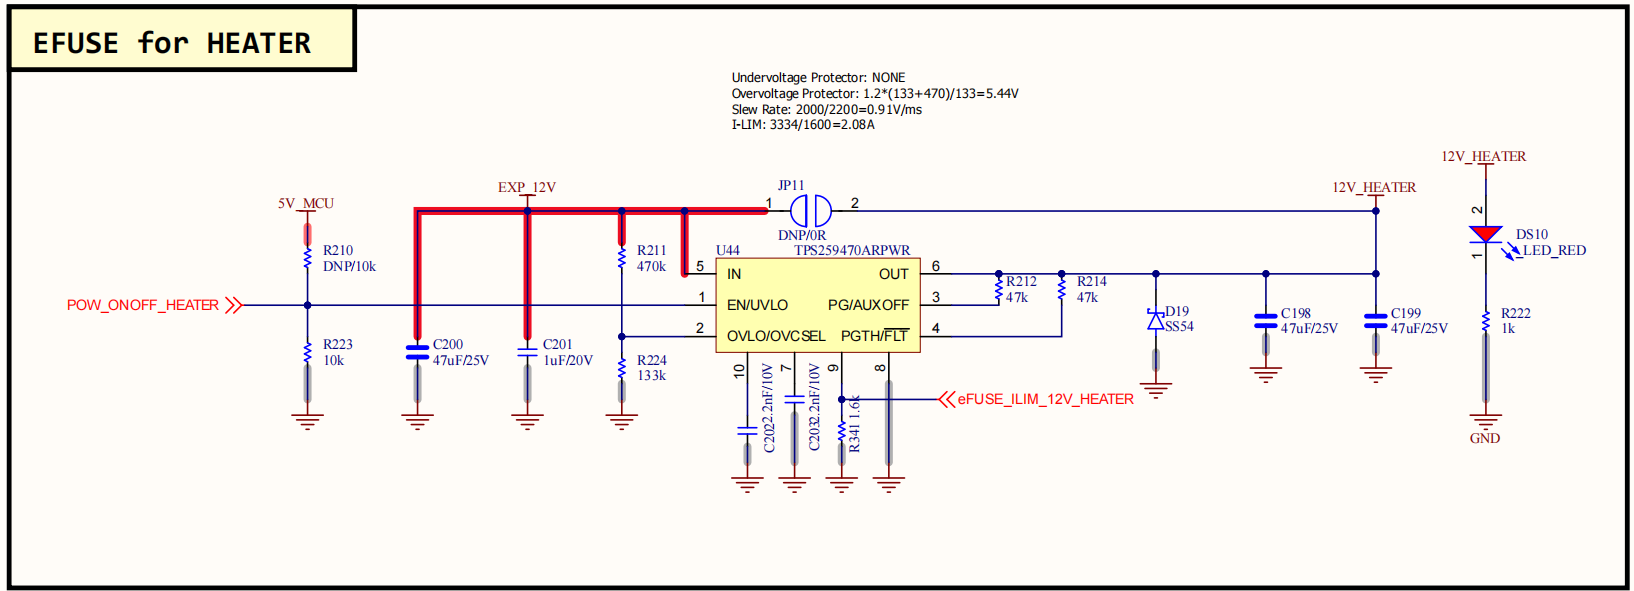
\includegraphics[width=0.48\textwidth]{picture/exp/efuse-12vexp-12vheater.png}}
    \\caption{Sơ đồ nguyên lí khối efuse}
    \label{fig:exp-efuse}
\end{figure}
\textbf{Chức năng:} Các eFuse (cầu chì điện tử) sử dụng IC TPS259470ARPWR có chức năng bảo vệ quá áp, thiếu áp và quá dòng. Ngưỡng bảo vệ có thể thiết lập bằng điện trở ngoài, đồng thời IC hỗ trợ xuất tín hiệu giám sát để MCU theo dõi trạng thái dòng/áp.

Theo datasheet TPS25947xx, ngoài ngưỡng khóa thấp mặc định nội bộ, chân \textit{EN/UVLO} còn cho phép đặt lại ngưỡng Undervoltage Protection thông qua cầu phân áp ngoài. Vì vậy ngưỡng điện áp vào kích hoạt bảo vệ có thể điều chỉnh theo yêu cầu thiết kế.

Quan hệ đặt ngưỡng UVLO:
\begin{equation}
V_{IN(UV)} = \frac{V_{UVLO}\times(R1+R2)}{R2}
\end{equation}

Trong đó \(V_{UVLO}\) là điện áp tham chiếu tại chân \textit{EN/UVLO} theo datasheet, \(R1\) là điện trở nối từ \(V_{IN}\) đến chân \textit{EN/UVLO}, và \(R2\) là điện trở nối từ chân \textit{EN/UVLO} xuống GND. Do đó có thể thay đổi tỉ số \(R1/R2\) để chọn ngưỡng điện áp thiếu áp phù hợp cho từng nhánh nguồn eFuse.

Tương tự, theo mục Overvoltage Lockout (OVLO) của TPS259470x/4x, ngưỡng bảo vệ quá áp được đặt tại chân \textit{OVLO} bằng cầu phân áp ngoài. Khi điện áp tại chân \textit{OVLO} vượt ngưỡng lên \(V_{OV(R)}\), eFuse sẽ ngắt nguồn ra để bảo vệ tải. Thiết bị chỉ cho phép bật lại khi điện áp giảm xuống dưới ngưỡng xuống \(V_{OV(F)}\), trong đó hai ngưỡng này khác nhau một khoảng nhỏ để tạo hysteresis, tránh đóng cắt liên tục khi tín hiệu vào dao động gần ngưỡng.

Quan hệ đặt ngưỡng OVLO:
\begin{equation}
V_{IN(OV)} = \frac{V_{OV}\times(R1+R2)}{R2}
\end{equation}

Với \(V_{OV}\) là điện áp tham chiếu của bộ so sánh OVLO theo datasheet. Như vậy, bằng cách chọn tỉ số \(R1/R2\), người thiết kế có thể chủ động đặt ngưỡng quá áp phù hợp để bảo vệ từng nhánh tải trong khối eFuse.

Bên cạnh đó IC còn hỗ trợ khả năng cấu hình ngưỡng dòng điện bằng việc cấu hình bằng điện trở ở chân I\textsubscript{LIM}, được xác đinh bởi công thức 
\begin{equation}
R_{ILIM}= \frac{3334}{I_{ILIM}} \,\Omega
\end{equation}

Từ vị trí chân đấy, có thể dùng để đọc về tín hiệu ADC tại đầu điện trở R\textsubscript{ILIM} để theo dõi được dòng điện tiêu thụ, từ đó giúp hệ thống vận hành ổn định và an toàn.

Ngoài những chức năng chính của efuse là bảo vệ quá dòng, quá áp, đặt các ngưỡng dòng áp cho mạch hoạt động, IC TPS259470ARPWR còn hỗ trợ việc người dùng có thể tùy ý điều chỉnh thời gian ngắt của efuse bằng một tụ điện nối vào chân ITIMER (pin 10) và kéo xuống đất. Trong thực tế việc cần thời gian ngắt dòng chứ không phải ngắt ngay lập tức mang lại nhiều ưu điểm cho mạch phía sau. Ví dụ như tránh false trigger vì tải có thể tạo ra những xung dòng ngắn (transient) khi khởi động hoặc khi chuyển trạng thái nếu IC cắt ngay lập tức, nó sẽ coi những xung ngắn này là lỗi và ngắt nguồn, gây reset hoặc mất ổn định cho hệ thống. Bảo vệ quá dòng kết hợp với bảo vệ sự ổn định của mạch, nếu dòng chỉ vượt ngưỡng trong thời gian ngắn thì không cần thiết phải đóng ngay hệ thống ngay lập tức, tụ chân 10 giúp duy trì một khoảng thời gian ngắt nếu dòng vượt ngưỡng hơn một khoảng thời gian cần thiết thì từ đó mới ngắt mạch.


\begin{equation}
t_{TIMER}(ms) = \frac{\Delta V_{ITIMER}(V) \times C_{TIMER}(nF)}{I_{TIMER}(\mu A)}
\end{equation}

Tương ứng với việc có thể ngắt dòng tùy theo thời gian thiết lập, IC cũng hỗ trợ khả năng làm mềm quá trình khởi động. Điều này liên quan đến 2 đại lượng ta phải quan tâm tại thời điểm mở nguồn đó là Inrush Current (dòng xung khi bật nguồn) và Slew Rate (dV/dt tốc độ tăng điện áp đầu ra khi IC bật). Thông thường những mạch có nhiều tải sẽ đi kèm với những tụ lọc nguồn ví dụ như ở các con MCU hay MPU, số lượn tụ lọc nguồn là rất nhiều, bên cạnh đó còn có các IC nhớ hay IC driver khác trong mạch. Với số lượng tụ lớn sẽ dễ tạo ra inrush current lớn ngay thời điểm bật nguồn, vì tại thời điểm khi có nguồn dòng nạp rất lớn sẽ chảy vào các tụ trong thời gian ngắn, dòng lớn này có thể gây sụt áp nguồn hay reset hệ thống. Bên cạnh đó khi điện áp đầu ra IC tại thời điểm bật tăng quá nhanh sẽ kéo dòng nạp tụ lớn hơn nữa (I = C × dV/dt), do đó IC cho phép khả năng điều chỉnh tốc độ tăng điện áp ngõ ra ở chân DVDT (pin 7) bằng việc đặt một tụ kéo xuống đất. Với công thức bên dưới.

\begin{equation}
SR(V/ms) = \frac{I_{INRUSH}(mA)}{C_{out}(\mu F)}
\end{equation}

\begin{equation}
C_{dvdt}(pF) = \frac{2000}{SR(V/ms)}
\end{equation}

\begin{figure}[H]
    \centering
    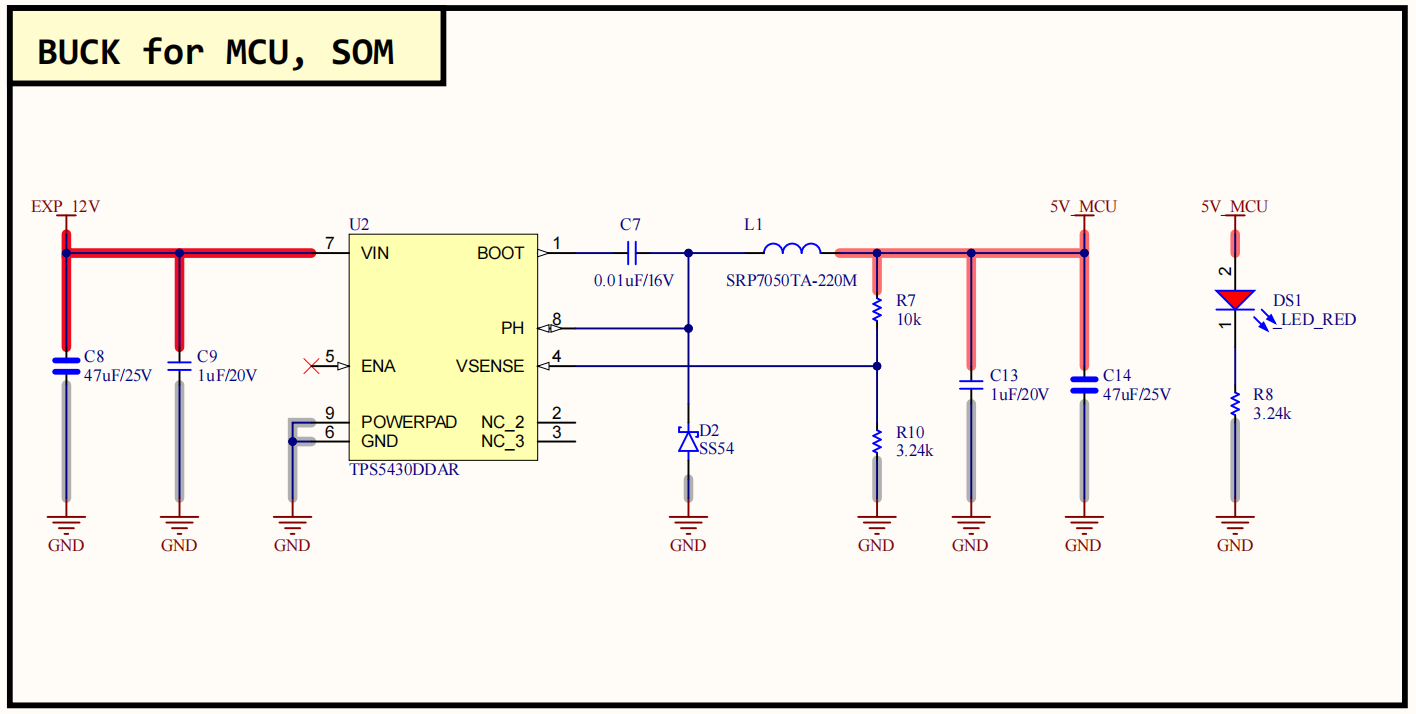
\includegraphics[width=0.8\textwidth]{picture/exp/buck-12vexp-5vmcu.png}\\
    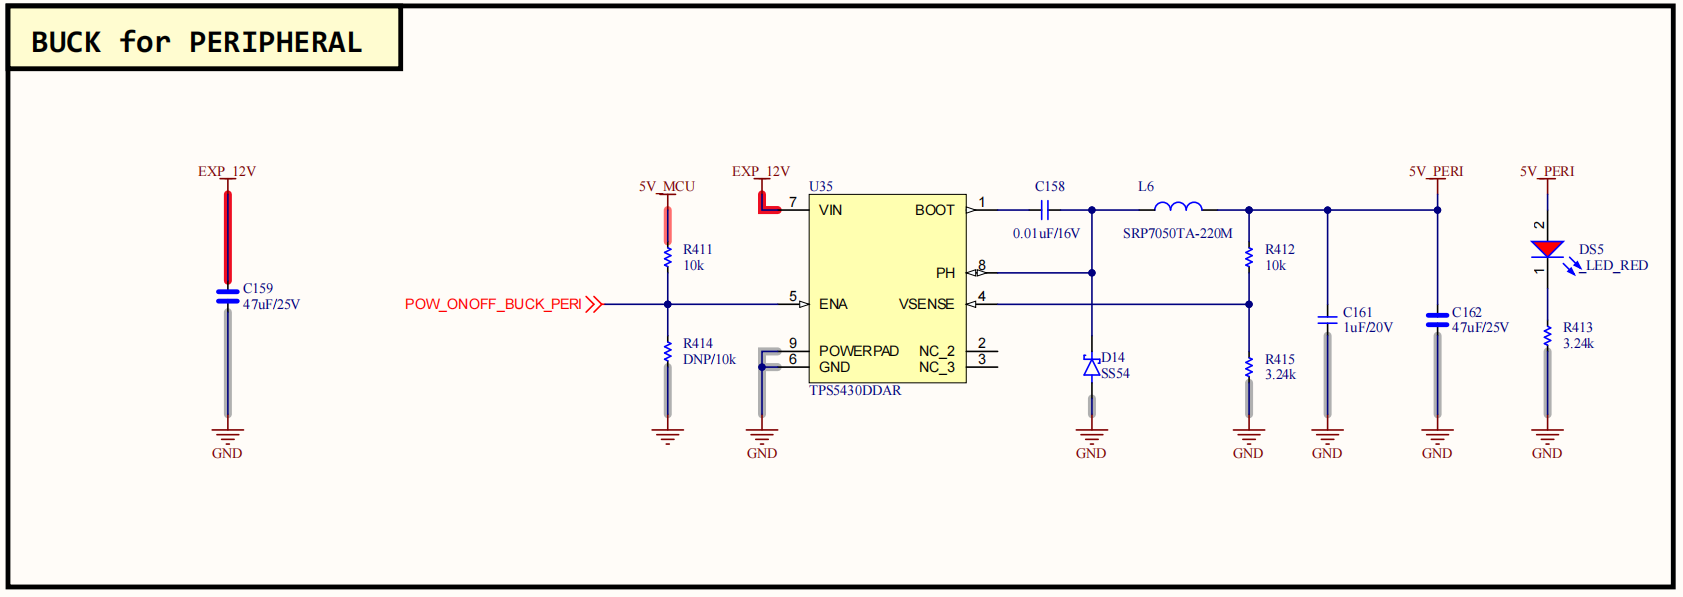
\includegraphics[width=0.8\textwidth]{picture/exp/buck-12vexp-5vperi.png}
    \\caption{Sơ đồ nguyên lí khối BUCK}
    \label{fig:exp-buck}
\end{figure}
Sử dụng mạch buck để hạ áp điện áp từ 12V nguồn chính xuống điện áp 5V sử dụng cho MPU, MCU và các IC chức năng khác. Mạch buck dùng khi cần hạ điện áp với một khoảng lớn, điều này sẽ ít hao phí hơn sử dụng LDO để hạ khoảng áp lớn. 

IC TPS5430DDAR có dãy điện áp ngõ vào rộng từ 5V5 đến 36V, cho phép dòng chảy liên tục tối đa lên đến 3A và dòng đỉnh tối đa 4A. Hiệu suất chuyển đổi của IC có thể đạt tới 95\% trong điều kiện hoạt động bình thường với điện trở nội Rds(on) trên mosfet là 100m $\Omega$. Ramp nội bộ 500 kHz làm chuẩn thời gian cho băm xung đầu ra từ việc dùng error voltage từ op-amp (khi so sánh VSENSE với điên áp tham chiếu) so sánh với ramp để tạo duty cycle. IC TPS5430DDAR có thể điều chỉnh điện áp ngõ ra dựa vào tổ hợp 2 giá trị điện trở ở cầu phân áp từ ngõ ra về chân VSENSE theo công thức bên dưới.

\begin{equation}
R2 = \frac{R1 \times 1.221}{V_{OUT}- 1.221} 
\end{equation}

Với R1 là điện trở chia áp kéo lên nguồn và R2 là điện trở chia áp kéo xuống đất, $V_{OUT}$ là điện áp ngõ ra mong muốn. Trong quá trình hoạt động ổn định, điện áp tại chân VSENSE phải bằng điện áp tham chiếu 1.221V

Ngõ vào $V_{in}$ thiết kế dùng 2 tụ lọc nguồn 47 $\mu F$ và 1 $\mu F$. Lí do sử dụng 2 tụ ngõ vào với 2 giá trị chênh lệch khá lớn là vì dùng tụ lớn với mục tiêu nạp/xả chậm, phản ứng tốt với dao động chậm, nhiễu ở tần số thấp, điện dung cao năng lượng được tích trữ lớn giúp giữ ổn định nguồn khi xảy ra sụt áp ở tải. Giá trị tụ nhỏ ngược lại sẽ giúp nạp/xả nhanh, phản ứng tốt với nhiễu ở tần số cao, dùng để triệt nhiễu switching, xung nhanh, hoặc làm tụ bypass gần IC.

Cuộn cảm ngõ ra được đặt để dập các gai dòng trên tụ điện gây ra, do khi mosfet đóng ngắt nhanh trong thời gian ngắn dẫn đến dòng qua tụ có biên độ lớn, cuộn cảm được sử dụng để giảm sự thay đổi nhanh dòng qua tụ. Giá trị cuộn cảm được đề xuất tính theo công thức 



\begin{equation}
L_{MIN} = \frac{V_{OUT(MAX)} \times (V_{IN(MAX)} - V_{OUT})}{V_{IN(MAX)} \times K_{IND} \times I_{OUT} \times F_{SW}}
\end{equation}

Trong thiết kế gốc, datasheet khuyến nghị sử dụng cuộn cảm khoảng 15 µH với hệ số KIND = 0.2. Tuy nhiên, do board mạch hiện có sẵn cuộn cảm 20 µH, giá trị này được lựa chọn để thuận tiện cho việc lắp ráp. Việc sử dụng cuộn cảm lớn hơn giúp giảm dòng gợn qua cuộn cảm, từ đó điện áp ripple đầu ra nhỏ hơn và mạch duy trì chế độ dẫn liên tục ở tải thấp. Nhược điểm là đáp ứng quá độ có thể chậm hơn so với giá trị 15 µH, nhưng vẫn đảm bảo nguyên lý hoạt động và độ tin cậy của hệ thống. Đây là sự đánh đổi hợp lý giữa điều kiện linh kiện thực tế và yêu cầu thiết kế.

Tụ đầu ra cần được lựa chọn dựa trên ba thông số quan trọng: điện áp DC định mức, khả năng chịu dòng gợn và điện trở tương đương ESR. Điện áp và dòng gợn không được vượt quá giới hạn của tụ, trong khi ESR cùng với dòng gợn qua cuộn cảm quyết định biên độ điện áp ripple đầu ra. Giá trị điện dung không cần chính xác tuyệt đối, nhưng phải đảm bảo mối quan hệ giữa tần số cắt LC của bộ lọc và tần số crossover của vòng điều khiển. Do đặc tính bù bên trong IC, tần số crossover nên nằm trong khoảng 3 kHz đến 30 kHz để có đủ độ lợi pha, đồng thời phải nhỏ hơn tần số zero do ESR của tụ. Trong thiết kế này, tần số crossover được chọn nằm trong khoảng 2.59 kHz đến 24 kHz, thỏa mãn các điều kiện trên và đảm bảo hệ thống hoạt động ổn định. Trong thiết kế tận dụng tụ đầu vào để áp dụng cho đầu ra nhưng vẫn phải đảm bảo phù hợp với ba thông số vừa liệt kê. Công thức chính xác để tính giá trị tụ được mô tả bên dưới dựa vào datasheet.

\begin{equation}
f_{CO} = \frac{f_{LC}^2}{85 \, V_{OUT}}
\end{equation}

\begin{equation}
C_{OUT} = \frac{1}{3357 \times L_{OUT} \times f_{CO} \times V_{OUT}}
\end{equation} 

Giữa chân BOOT và PH dùng 1 tụ điện cemeamic nối tiếp với ngõ ra có giá trị 0.01 $\mu F$. Tụ này cung cấp điện áp điều khiển cho MOSFET phía cao. Giá trị 0.01 $\mu F$ vừa đủ để nạp/giữ điện áp gate trong mỗi chu kỳ chuyển mạch. Nếu tụ quá lớn thì tốc độ nạp/xả chậm, làm giảm hiệu quả chuyển mạch. Nếu tụ quá nhỏ thì không giữ được điện áp gate ổn định. 0.01 $\mu F$ là giá trị tối ưu mà hãng đã thử nghiệm, đảm bảo MOSFET high-side bật/tắt nhanh, giảm tổn hao chuyển mạch, đồng thời không gây dao động hay trễ.

Trong mạch TPS5430, cần sử dụng một diode bắt (catch diode) ngoài giữa chân PH và GND. Diode này phải đáp ứng các điều kiện tuyệt đối của ứng dụng: điện áp ngược phải lớn hơn điện áp cực đại tại chân PH (VIN(MAX) + 0.5 V), dòng đỉnh phải lớn hơn IOUT(MAX) cộng với một nửa dòng gợn qua cuộn cảm, và điện áp rơi thuận phải nhỏ để đạt hiệu suất cao. Thời gian dẫn của diode thường dài hơn thời gian MOSFET high-side bật, do đó việc chọn diode phù hợp có thể cải thiện đáng kể hiệu suất tổng thể. Ngoài ra, cần đảm bảo diode có khả năng tản nhiệt cho công suất hao phí. Trong thiết kế này, linh kiện SS54 được sử dụng, với điện áp ngược 40 V, dòng thuận 5 A và điện áp rơi thuận thấp, đáp ứng tốt các yêu cầu trên và đảm bảo hiệu suất cũng như độ tin cậy của hệ thống.

Chân ENA cung cấp điều khiển bật và tắt điện áp cho bộ điều chỉnh. Khi điện áp chân ENA vượt quá điện áp ngưỡng, bộ điều chỉnh bắt đầu hoạt động và chế độ khởi động chậm nội bộ bắt đầu tăng dần. Nếu điện áp chân ENA bị kéo xuống dưới điện áp ngưỡng, bộ điều chỉnh sẽ dừng việc chuyển đổi và chế độ khởi động chậm nội bộ sẽ được thiết lập lại. Nối chân này với đất hoặc bất kỳ điện áp nào thấp hơn 0,5V sẽ vô hiệu hóa bộ điều chỉnh và kích hoạt chế độ tắt. Dòng điện không tải của TPS543x trong chế độ tắt thông thường là 15$\mu A$.

Bên cạnh việc thiết kết chủ động từ việc dùng các giá trị điện trở, tụ điện, cuộn cảm để thực hiện được giá trị ngõ ra mong muốn, nội bộ IC còn hỗ trợ một số chức năng giúp bảo vệ IC, bảo vệ hệ thống, giúp hệ thống hoạt động ổn định. Ví dụ như khả nănh bảo vệ quá dòng, bằng cách giám sát điện áp drain–source của MOSFET. Khi dòng vượt ngưỡng, mạch sẽ ngắt MOSFET trong chu kỳ hiện tại (cycle-by-cycle limiting). Trong trường hợp ngắn mạch, thiết bị chuyển sang chế độ hiccup, tạm ngừng hoạt động rồi khởi động lại sau thời gian trễ. Nhờ đó, IC được bảo vệ khỏi hư hỏng và hệ thống duy trì độ tin cậy. Cùng với việc bảo vệ quá dòng, IC cũng tích hợp bảo vệ quá áp bằng cách giám sát điện áp hồi tiếp tại chân VSENSE. Khi điện áp này vượt quá $112.5 \%$ giá trị tham chiếu, MOSFET high-side sẽ bị ngắt để tránh hiện tượng overshoot. Khi điện áp giảm xuống dưới ngưỡng, MOSFET được kích hoạt trở lại. Cơ chế này giúp bảo vệ tải và nâng cao độ tin cậy của hệ thống. Trong môi trường không gian với các mức nhiệt độ khắc nghiệt, đòi hỏi một hệ thống phải có khả năng cảm nhận được nhiệt độ và có những cơ chế bảo vệ thích nghi với điều từ nhiệt độ môi trường cũng như là nhiệt độ hoạt động của linh kiện, IC tích hợp mạch bảo vệ nhiệt nhằm ngăn chặn hư hỏng khi nhiệt độ junction vượt ngưỡng cho phép. Khi nhiệt độ vượt ngưỡng, điện áp tham chiếu bị ngắt và MOSFET high-side tắt. Thiết bị sẽ tự động khởi động lại khi nhiệt độ giảm xuống thấp hơn ngưỡng khoảng 14°C, dưới sự kiểm soát của mạch slow-start. Cơ chế này đảm bảo IC hoạt động an toàn và ổn định trong điều kiện môi trường khắc nghiệt.

\begin{figure}[H]
    \centering
    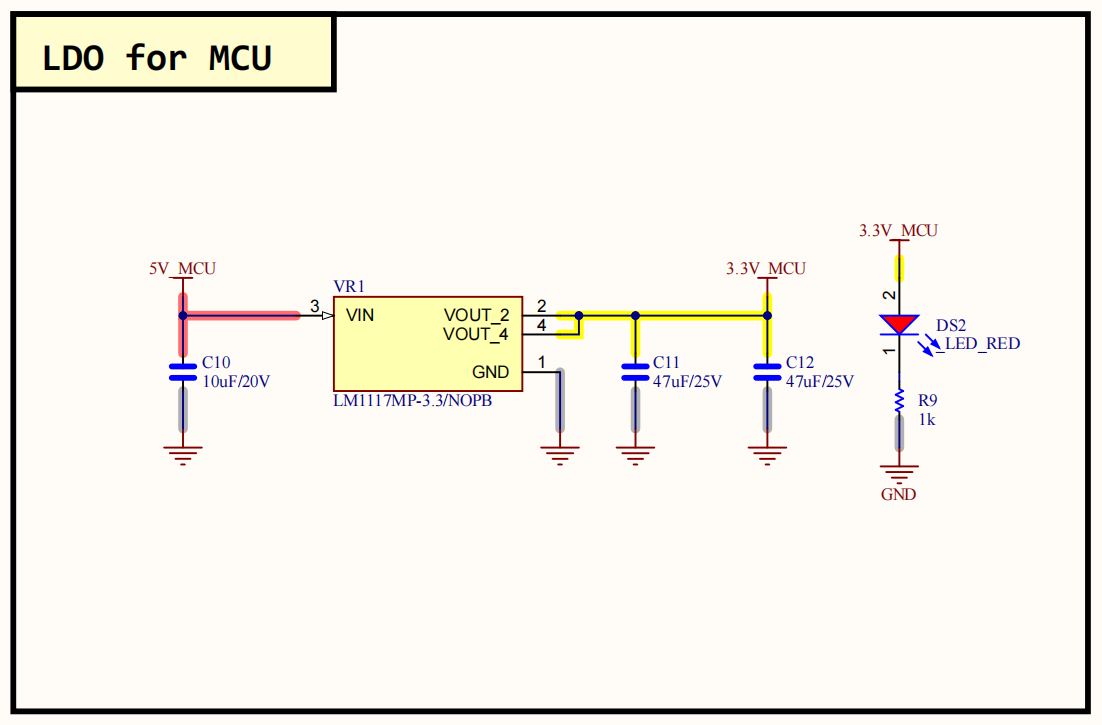
\includegraphics[width=0.8\textwidth]{picture/exp/ldo-5vmcu-3v3muc.png}\\
    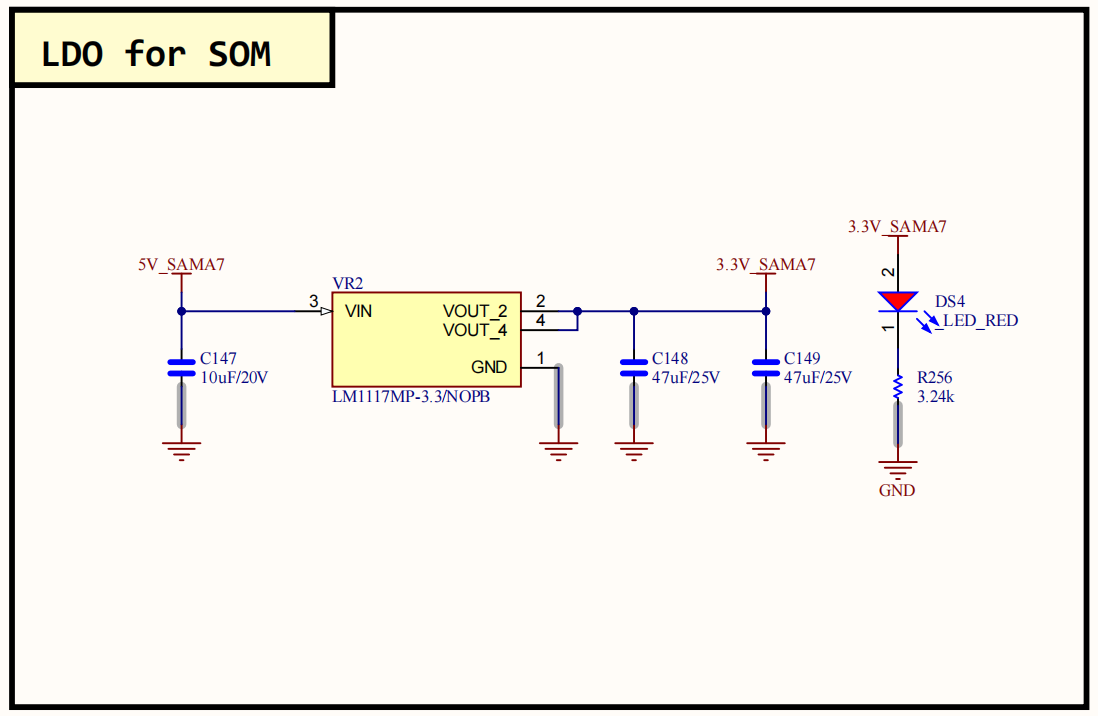
\includegraphics[width=0.8\textwidth]{picture/exp/ldo-5vsam-3v3sam.png}\\
    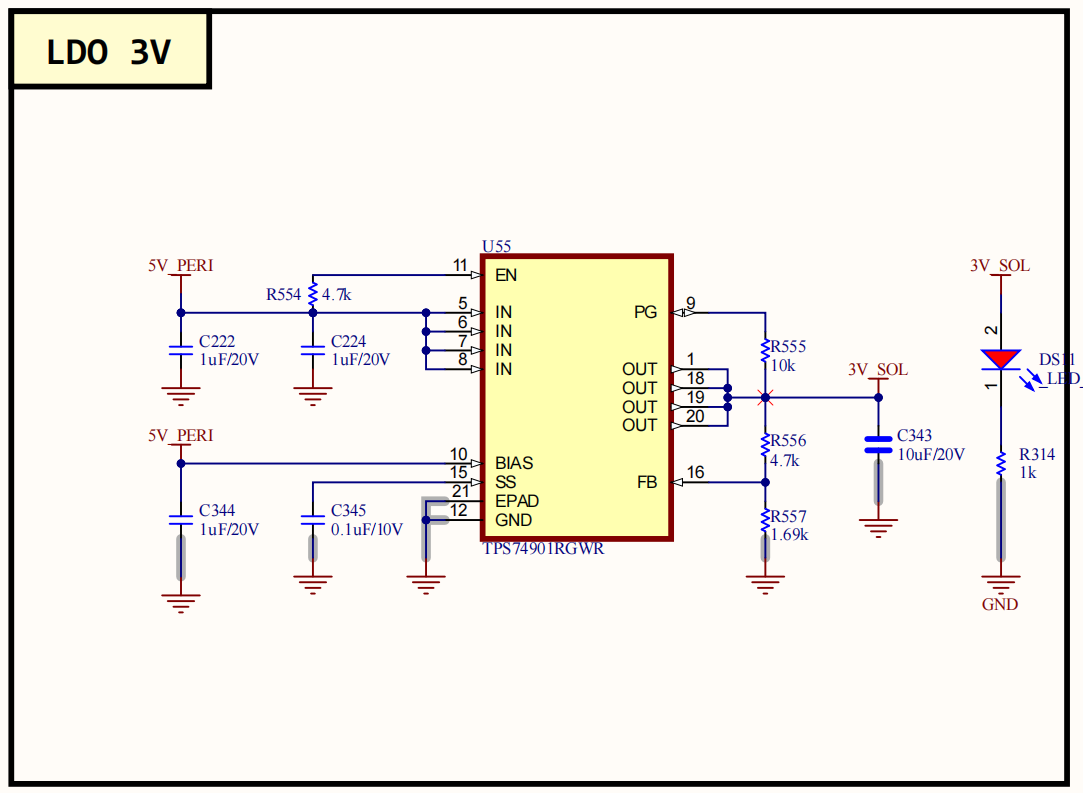
\includegraphics[width=0.8\textwidth]{picture/exp/ldo-3vsol.png}
    \\caption{Sơ đồ nguyên lí khối LDO}
    \label{fig:exp-ldo}
\end{figure}

Sử dụng mạch LDO để hạ áp điện áp từ 5V xuống điện áp 3V3 sử dụng cho MPU, MCU và các IC chức năng khác. Với khoảng rơi áp khá nhỏ ta dùng nguồn ldo thay vì nguồn buck, việc sử dụng LDO sẽ làm cho nguồn ra ổn định hơn so với buck

LM1117 là IC ổn áp tuyến tính low-dropout có khả năng cung cấp dòng tải đến 800 mA với điện áp rơi thấp, đảm bảo điện áp ra ổn định và chính xác (sai số ±1$\%$). Thiết bị hỗ trợ nhiều mức điện áp cố định và chỉnh được, tích hợp bảo vệ quá nhiệt và giới hạn dòng, đồng thời dễ thiết kế nhờ các package nhỏ gọn. Đây là lựa chọn phổ biến cho nguồn trong thiết bị công nghiệp, server và làm post-regulator cho DC/DC converter.

Các tụ lọc ngõ vào và ngõ ra lựa chọn giá trị 10 $\mu F$ và 47 $\mu F$, các giá trị tụ không bắt buộc các giá trị chính xác, chọn phù hợp với thiết kế và tận dụng các thiết kế có sẵn.

Bên cạnh IC LM1117 còn dùng TPS74901. So với các LDO thông thường, TPS74901 có nhiều ưu điểm nổi bật. Thiết kế sử dụng NMOS pass transistor giúp đạt dropout rất thấp (chỉ khoảng 120 mV ở 3A), đồng thời hỗ trợ nguồn bias riêng (VBIAS) để duy trì đáp ứng nhanh ngay cả khi điện áp đầu vào thấp. Thiết bị còn có soft‑start lập trình được, giảm dòng xung khi khởi động và hỗ trợ sequencing nhiều rail nguồn nhờ ngõ ra power‑good. Ngoài ra, TPS74901 ổn định với mọi loại tụ ≥ 2.2 µF, có độ chính xác cao ±1$\%$, độ nhiễu thấp phù hợp cho mạch nhạy cảm, và được đóng gói trong kích thước nhỏ gọn. Những đặc điểm này khiến TPS74901 trở thành giải pháp LDO cao cấp, vượt trội hơn so với các LDO truyền thống vốn chỉ đáp ứng cơ bản về ổn áp.

Bên cạnh khối PMIC, trong hệ sinh thái quản lý nguồn còn có thêm khối power measurement and distribution, khối này có đầu vào từ các điện trở shunt mắc nối tiếp tại các mức nguồn phát. Mục tiêu là đo được điện áp trên trở shunt từ đó theo dõi được dòng điện tiêu thụ trên mỗi nguồn áp. Trong thiết kế sử dụng 4 điện trở shunt với giá trị khá nhỏ là 0.01R để tránh rơi áp không cần thiết. Các dòng tiêu thụ được đo là các dòng từ VDDCORE (1V15 cho 1 số chân VDDCORE của MPU), VDDCPU (1V15 cho 1 số chân VDDCPU của MPU), VDD3V3 (nguồn cấp cho các chân IO của MPIU cũng như một số chân nguồn cần 3V3) và VDD\_1V35 (dùng cho mức điện áp giao tiếp với IC RAM DDR3).

\begin{figure}[H]
    \centering
    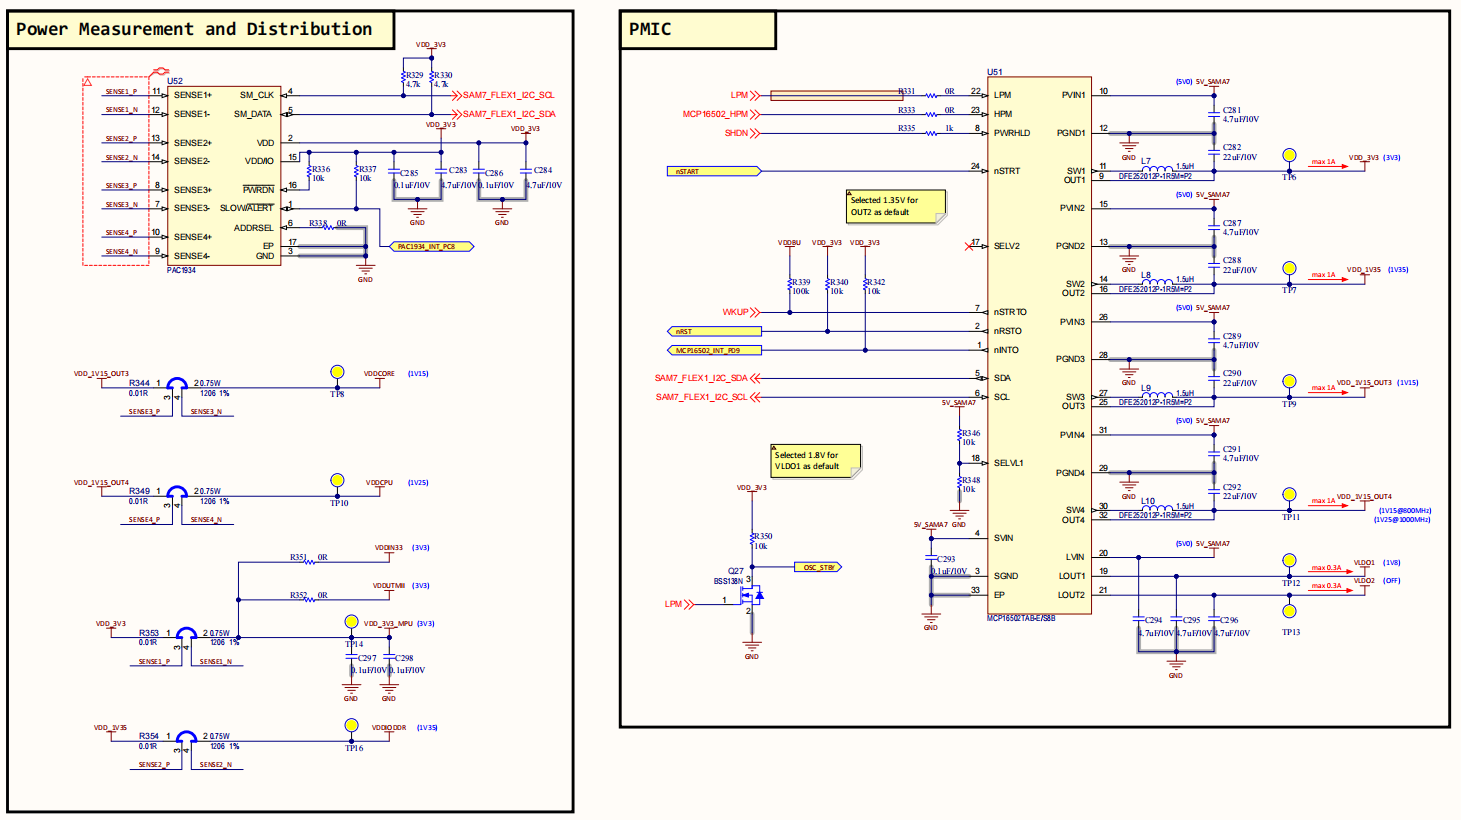
\includegraphics[width=1\textwidth]{picture/exp/khoi-pmic.png}
    \\caption{Sơ đồ nguyên lí khối PMIC và giám sát dòng}
    \label{fig:exp-sche-khoi-pmic}
\end{figure}

MCP16502 là một IC quản lý nguồn tích hợp (PMIC) của Microchip, được thiết kế để phối hợp tối ưu với các dòng vi xử lý SAM như SAMA5D2, SAM9X6/7 và SAMA7G5. Con chip này cho phép cung cấp nhiều rail nguồn trong một giải pháp duy nhất, giúp giảm số lượng linh kiện rời và đơn giản hóa thiết kế hệ thống. MCP16502 hỗ trợ đầu vào từ 2.7V đến 5.5V, tích hợp 4 bộ chuyển đổi DC-DC Buck (mỗi kênh đến 1A) và 2 LDO (mỗi kênh đến 300 mA), đảm bảo hiệu suất cao và độ chính xác điện áp ±1\% cho các rail quan trọng như CPU và DDR. Ngoài ra, nó còn hỗ trợ giao tiếp I²C để cấu hình và giám sát, có các chế độ năng lượng linh hoạt (Hibernate, Low-Power, High-Performance) cùng khả năng điều chỉnh điện áp động (DVS). Có các tính năng bảo vệ như chống quá nhiệt, giới hạn dòng và ESD. MCP16502 được thiết kế để dùng với hệ sinh thái SAM, khi nó cung cấp trực tiếp các rail điện áp cần thiết và đồng bộ tín hiệu điều khiển với MPU giúp cho khả năng thiết kế, sử dụng và bảo trì được thuận lợi hơn.

Các mode hoạt động của IC MCP16502:

\begin{itemize}
    \item \textbf{High-Performance Mode:} cung cấp đầy đủ điện áp và dòng tải cho MPU khi chạy ở mức hiệu năng cao. Được điều khiển bởi tín hiệu HPM từ MCU

    \item \textbf{Low-Power Mode:} giảm điện áp và tần số hoạt động để tiết kiệm năng lượng khi hệ thống không cần xử lý nặng. Được điều khiển bởi tín hiệu LPM của MCU
    
    \item \textbf{Hibernate Mode:} đưa hệ thống vào trạng thái ngủ sâu, tiêu thụ điện năng cực thấp, chỉ giữ các rail cần thiết để MPU có thể khởi động lại nhanh.

    \item \textbf{Dynamic Voltage Scaling (DVS):} cho phép thay đổi điện áp động theo nhu cầu xử lý của MPU, giúp cân bằng giữa hiệu năng và tiết kiệm năng lượng.
\end{itemize}

Tại các kênh ngõ ra cổng buck, sử dụng cuộn cảm với giá trị 1.5 $\mu$H để dập các dòng vọt như thiết kế ở các mạch buck thông thường.

Tại vị trí sau cuộn dây cũng có các tụ decoupling và bypass để làm ổn định tín hiệu ngõ ra.

IC MCP16502 hỗ trợ giao thức I2C có thể đạt tốc độ 1MHz để giao tiếp với MPU bởi địa chỉ 0x5B. MPU giao tiếp với I2C để thực hiện một số thiết lập như cấu hình các thông số hoạt động của các kênh nguồn (ví dụ như điện áp đầu ra VSET, trạng thái bật tắt nguồn, chế độ hoạt động, tốc độ thay đổi điện áp DVS). MPU cũng có thể giám sát trạng thái vào ghi nhận lỗi gửi về từ MCP16502 như trạng thái lỗi: Kiểm tra các cờ báo lỗi như lỗi nhiệt (TSD), cảnh báo nhiệt (TWR), hoặc lỗi quá dòng trên từng kênh (FLT, HICCUP), trạng thái nguồn ổn định (POK), xử lý ngắt.

\textbf{Tính toán từ schematic (khi có R shunt/điện áp đo):}
\[
    I_{rail}=\frac{V_{SHUNT}}{R_{SHUNT}}, \qquad P_{load}=V_{rail}\cdot I_{rail}
\]
\textit{Cách tính:} lấy \(R_{SHUNT}\) và điện áp rơi trên shunt đúng theo giá trị ghi trên hình, thay trực tiếp vào công thức để ra dòng và công suất từng rail.

\begin{figure}[H]
    \centering
    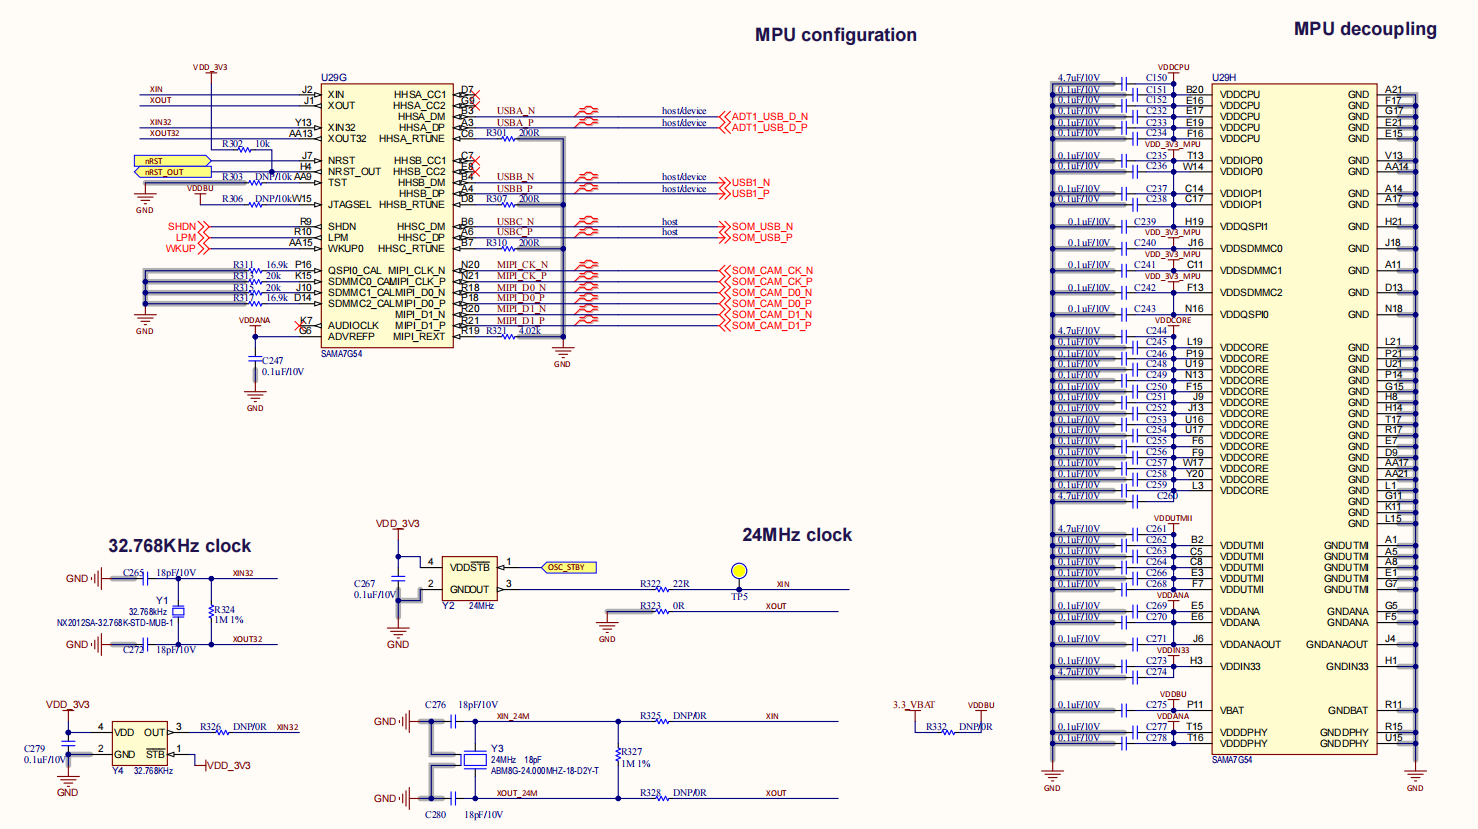
\includegraphics[width=1\textwidth]{picture/exp/khoi-sam-mpu.png}
    \\caption{Sơ đồ nguyên lí khối nguồn và tín hiệu tốc độ cao SAMA7G54 (MPU)}
    \label{fig:exp-sche-khoi-nguon-tin-hieu-sam-mpu}
\end{figure}

MPU SAMA7G54 dùng 2 nguồn xung ngoài là xung 24MHz và 32.768KHz, mỗi tần số có thể được tạo bởi thạch anh và bộ dao động, trong thiết kế sử dụng thạch anh là mặc định còn bộ dao động là DNP. 

Ở khối U29G thể hiện các tín hiệu tốc độ cao được kết nối từ chân MPU như trong hình như: camera (MIPI\_D/N), USB (USBA,B,C trong đó USB C là USB host only). Một số tín hiệu được điều khiển cho chức năng nguồn như SHDN, LPM, WKUP, nRST.

Khối U29H là các chân nối lên nguồn và nối đất, các chân nối nguồn được thiết kế với các tụ decoupling và bypass. Trên vi xử lý SAMA7G5, hệ thống nguồn được chia thành nhiều miền điện áp khác nhau để tối ưu hiệu năng và tiết kiệm năng lượng. Các mức chính bao gồm: nguồn 3.3 V (VDDIN33) cho nhiều khối I/O và làm đầu vào cho các bộ điều chỉnh nội bộ; nguồn 2.5 V (VDDOUT25) từ LDO bên trong phục vụ các khối analog và PLL; nguồn lõi 0.9–1.2 V (VDDCPU/VDDCORE) cho nhân Cortex-A7 và logic tốc độ cao, có hỗ trợ điều chỉnh động; nguồn 1.8 V hoặc 3.3 V (VDDANA) cho các khối analog như ADC và PLL; nguồn 1.8–3.3 V (VDDBU/VBAT) cho RTC và SRAM backup; các rail VDDIOPx có thể chọn 1.8 V hoặc 3.3 V để tương thích với ngoại vi; nguồn 1.2–1.5 V (VDDIODDR) cho DDR PHY; và nguồn 1.8 V (VDDUTMI) cho USB PHY. Như vậy, MPU này sử dụng nhiều mức điện áp từ 0.9 V đến 3.3 V, mỗi mức phục vụ cho một miền chức năng riêng biệt nhằm đảm bảo hoạt động ổn định và hiệu quả. Các nguồn này được tạo ra bởi một IC MCP16502 QFN-32 tạo nguồn chuyên biệt được thiết kế để cung cấp và theo dõi nguồn trên MPU. 

Để đảm bảo các thành phần hoạt động ổn định, một số chân tín hiệu được kéo trở nối đất sử dụng các giá trị trở được đề xuất theo tài liệu của chip và board EVK của nhà sản xuất.

\begin{figure}[H]
    \centering
    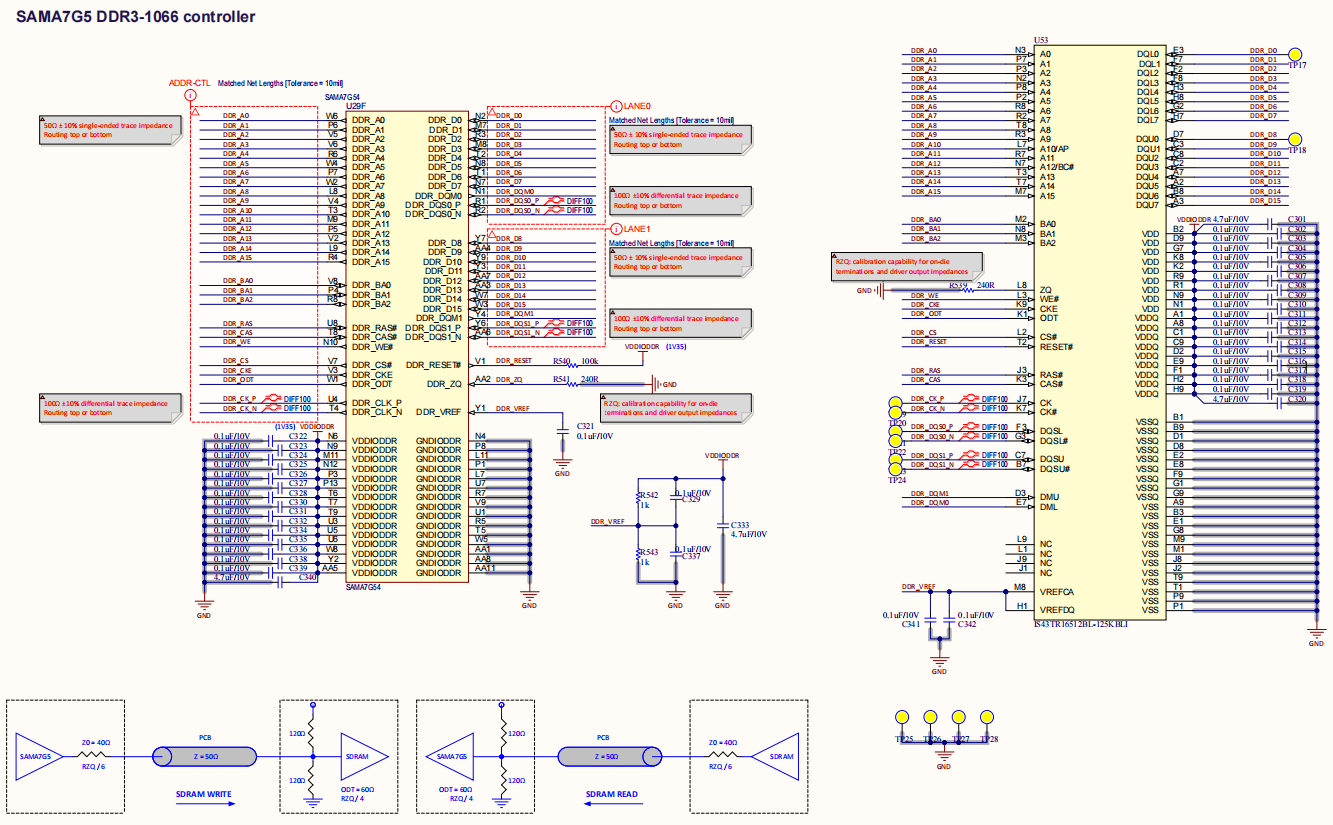
\includegraphics[width=1\textwidth]{picture/exp/khoi-sam-ddr3.png}
    \\caption{Sơ đồ nguyên lí khối DDR3 cho SAMA7G54}
    \label{fig:exp-sche-khoi-sam-ddr3}
\end{figure}

Tổng quan về IC RAM IS43TR16512BL của ISSI là một chip DDR3L SDRAM dung lượng 8Gb, được thiết kế để cung cấp hiệu năng cao và tiêu thụ điện năng thấp. Đây là loại bộ nhớ động đồng bộ tốc độ cao, hoạt động ở điện áp 1.35V, tương thích ngược với DDR3 1.5V. Với tốc độ truyền dữ liệu lên đến DDR3-1866, nó đáp ứng tốt nhu cầu băng thông của các hệ thống nhúng hiện đại. Bộ nhớ DDR3L được tổ chức thành nhiều bank, mỗi bank gồm nhiều hàng và cột. Khi CPU truy xuất, RAM sẽ chọn bank, hàng, rồi cột để đọc/ghi dữ liệu. Các thông số timing quan trọng như CAS Latency (CL), RAS to CAS Delay (tRCD), Row Precharge Time (tRP), và Row Active Time (tRAS) quyết định độ trễ và hiệu năng của RAM.

Một trong những ưu điểm nổi bật của RAM này là khả năng tiết kiệm năng lượng nhờ điện áp thấp, rất phù hợp cho các ứng dụng công nghiệp và thiết bị nhúng cần hoạt động lâu dài. Ngoài ra, dung lượng 8Gb đủ lớn để xử lý các tác vụ phức tạp như multimedia, giao tiếp tốc độ cao, hoặc chạy hệ điều hành nhúng. Chip cũng hỗ trợ nhiều tính năng nâng cao như tự động refresh, partial array self refresh, và on-die termination giúp cải thiện độ ổn định tín hiệu.

Các tín hiệu chính của DDR3 SDRAM bao gồm nhóm nguồn và clock (VDD, VDDQ, CK, CK\#), nhóm địa chỉ và bank (A0–A15, BA0–BA2), nhóm điều khiển (RAS\#, CAS\#, WE\#, CS\#, CKE, RESET\#), nhóm dữ liệu (DQ[0–15], DQS, DQS\#), cùng các tín hiệu hỗ trợ như ODT, ZQ, DM. Mỗi tín hiệu có chức năng riêng: ví dụ DQ truyền dữ liệu, DQS đồng bộ dữ liệu, RAS/CAS/WE điều khiển truy xuất bộ nhớ, còn ODT giúp điều chỉnh trở kháng để giảm phản xạ tín hiệu.

Về trở kháng đường truyền, DDR3 thường yêu cầu thiết kế PCB với trở kháng vi sai khoảng 100 Ω cho các cặp tín hiệu như DQS và CK, trong khi các đường dữ liệu đơn lẻ (DQ) thường nằm trong khoảng 50 $\Omega$. Chip hỗ trợ cấu hình driver strength và on-die termination để khớp trở kháng, đảm bảo tín hiệu ổn định khi truyền ở tốc độ cao.

Các tín hiệu chính của DDR3 SDRAM bao gồm nhóm nguồn và clock (VDD, VDDQ, CK, CK\#), nhóm địa chỉ và bank (A0–A15, BA0–BA2), nhóm điều khiển (RAS\#, CAS\#, WE\#, CS\#, CKE, RESET\#), nhóm dữ liệu (DQ[0–15], DQS, DQS\#), cùng các tín hiệu hỗ trợ như ODT, ZQ, DM. Mỗi tín hiệu có chức năng riêng: ví dụ DQ truyền dữ liệu, DQS đồng bộ dữ liệu, RAS/CAS/WE điều khiển truy xuất bộ nhớ, còn ODT giúp điều chỉnh trở kháng để giảm phản xạ tín hiệu.

\begin{figure}[H]
    \centering
    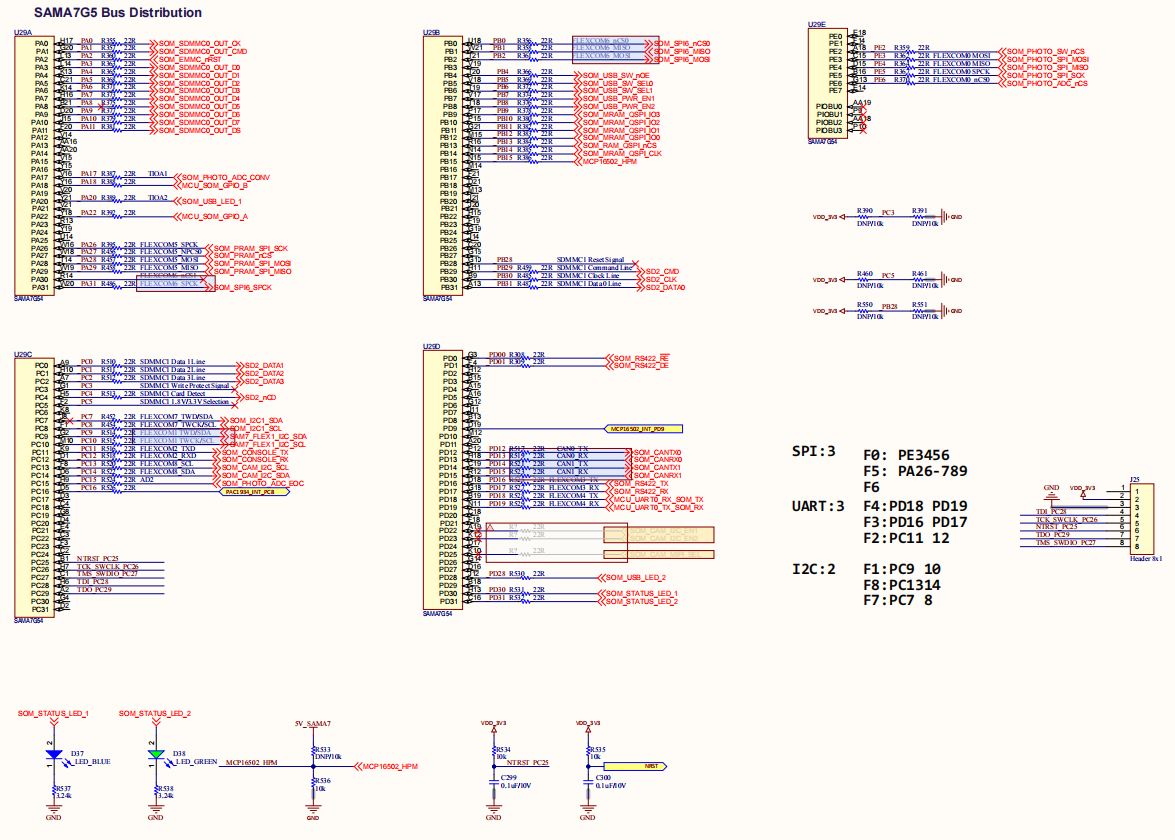
\includegraphics[width=1\textwidth]{picture/exp/khoi-sam-pio.png}
    \\caption{Sơ đồ nguyên lí khối chân PIO của SAMA7G54}
    \label{fig:exp-sche-khoi-sam-pio}
\end{figure}

Các chân tín hiệu I/O của SAMA7G54 kết nối đến các ngoại vi được thể hiện trong Hình \\ref{fig:exp-sche-khoi-sam-pio}.

Các tín hiệu ngoại vi chính của MPU gồm:
\begin{itemize}
    \item Giao thức SDMMC được sử dụng để kết nối với eMMC và thẻ nhớ SD Card, ở đây sử dụng SDMMC0 của MPU cho eMMC chi tiết ở bên dưới (hình \ref{fig:exp-sche-khoi-emmc}) và SDMMC1 cho thẻ SD Card chi tiết ở hình (hình \ref{fig:exp-sche-sdcard}) .
    \item MPU giao tiếp với một IC PRAM (hình \ref{fig:exp-sche-pram}); IC này giao tiếp với MPU thông qua SPI. Khối PRAM sẽ được trình bày chi tiết ở phần tương ứng.
    \item Bên cạnh PRAM, MPU còn giao tiếp với một IC MRAM (hình \ref{fig:exp-sche-mram-mpu}); MRAM giao tiếp với MPU bằng QSPI giúp tăng tốc độ đọc ghi dữ liệu. Chi tiết của MRAM sẽ được trình bày bên dưới (hình \ref{fig:exp-sche-mram-mpu}).
    \item Một IC RAM khác cũng được dùng là FRAM, FRAM được thiết kế để giao tiếp bằng giao thức SPI, nhưng trong thiết kế này do giới hạn về số lượng ngoại vi nên sử dụng USART để giao tiếp với FRAM thay vì SPI sẵn có của IC. Chi tiết về FRAM được trình bày ở bên dưới hình (hình \ref{fig:exp-sche-fram}).
    \item Giao thức I2C được dùng trong 2 mục đích chính là giao tiếp với các IC nội bộ trên board như IC theo dõi nguồn PAC1934 UQFN-16. Nối ra connector để giao tiếp với các board khác như connetor lên board camera, connector với board OBC.
    \item Giao thức SPI bên cạnh việc dùng cho các IC có chức năng nhớ còn dùng để đưa ra connector với board photo.
    \item Giao thức UART được dùng trong việc giao tiếp giữa core A (MPU) và core M (MCU), kéo ra connector RS422 được lái bởi IC transceiver UART-RS422, và một UART được kéo ra cho việc debug.
    \item Tín hiệu CAN TX/RX thông qua IC CAN transceiver để chuyển đổi lớp vật lí kéo ra bus CAN H/L chung để giao tiếp với MCU trên board và với connector ra board OBC.
    \item Các tín hiệu JTAG debug
\end{itemize}

Bên cạnh đó còn một số tín hiệu IO khác ví dụ như các IO dùng cho chức năng enable IC, một số thì dùng làm các tín hiệu select cho các IC switch, một số là khiển các led status, một số khác là các tín hiệu ngắt để nhật các sự kiện ngắt từ IC.

\begin{figure}[H]
    \centering
    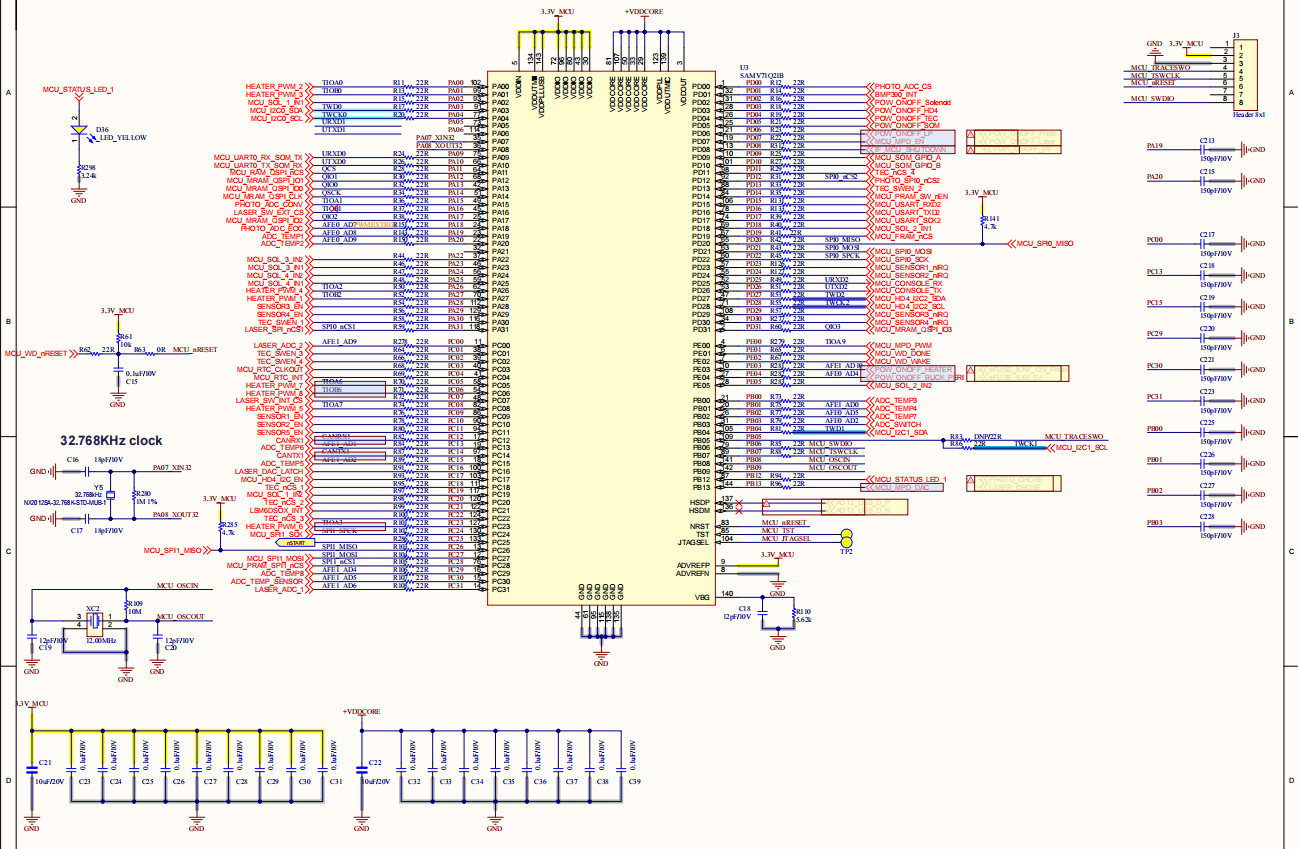
\includegraphics[width=1\textwidth]{picture/exp/khoi-mcu.png}
    \\caption{Sơ đồ nguyên lí khối MCU SAMV71Q21B}
    \label{fig:exp-sche-khoi-mcu}
\end{figure}
\textbf{Chức năng:} MCU SAMV71Q21B xử lý các tác vụ thời gian thực, đọc cảm biến và điều khiển tải chấp hành với độ trễ thấp, đồng thời trao đổi dữ liệu với MPU.

\begin{figure}[H]
    \centering
    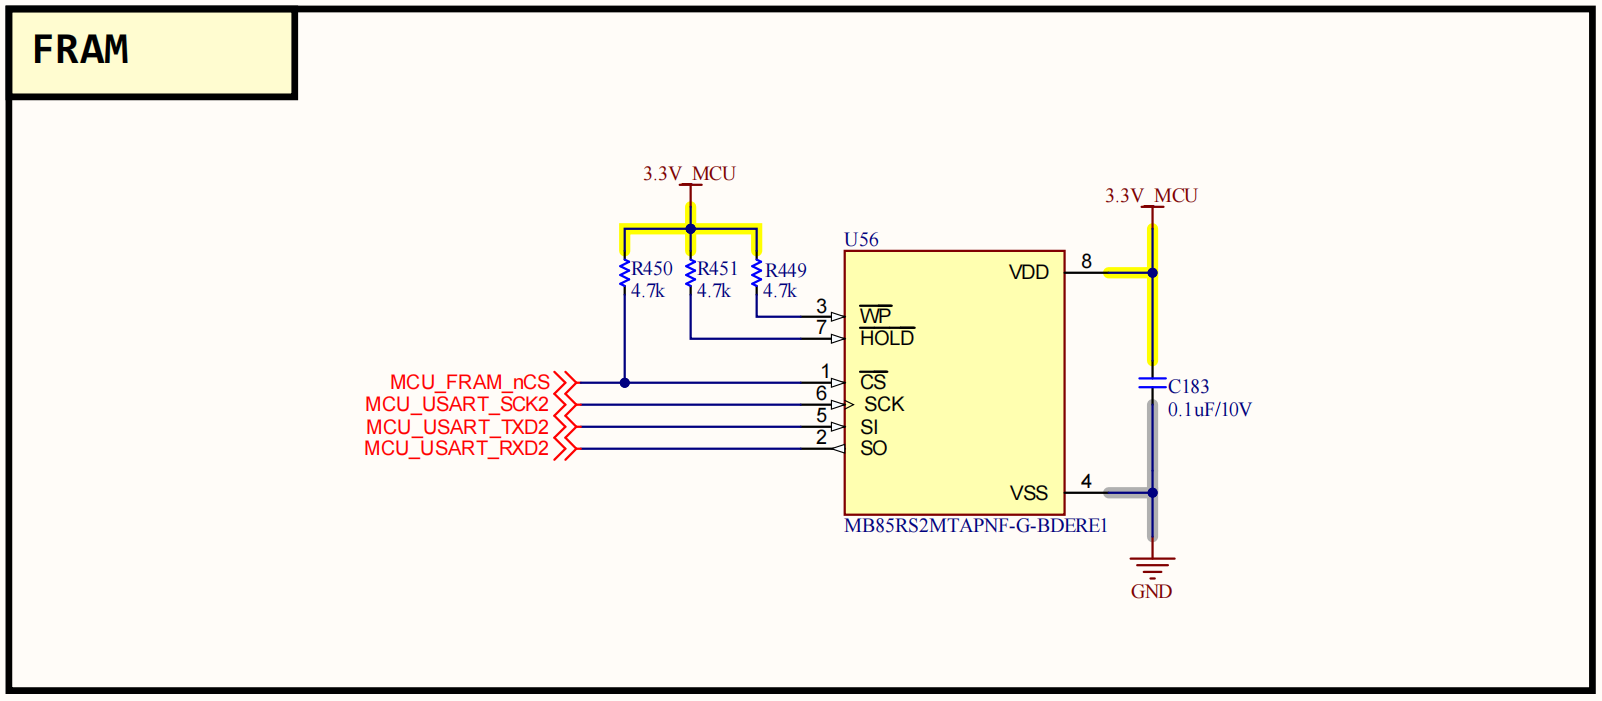
\includegraphics[width=1\textwidth]{picture/exp/fram.png}
    \\caption{Sơ đồ nguyên lí khối FRAM}
    \label{fig:exp-sche-fram}
\end{figure}

\begin{figure}[H]
    \centering
    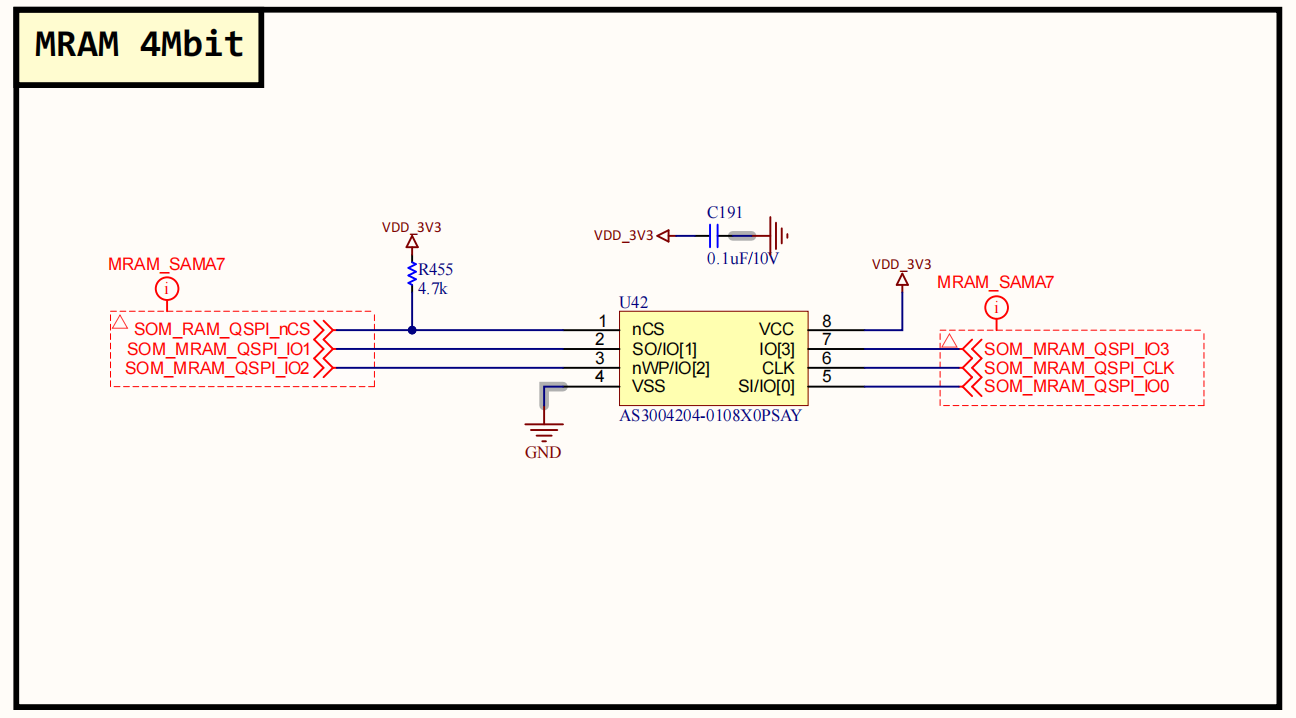
\includegraphics[width=1\textwidth]{picture/exp/mram-mpu.png}
    \\caption{Sơ đồ nguyên lí khối MRAM kết nối MPU}
    \label{fig:exp-sche-mram-mpu}
\end{figure}

\begin{figure}[H]
    \centering
    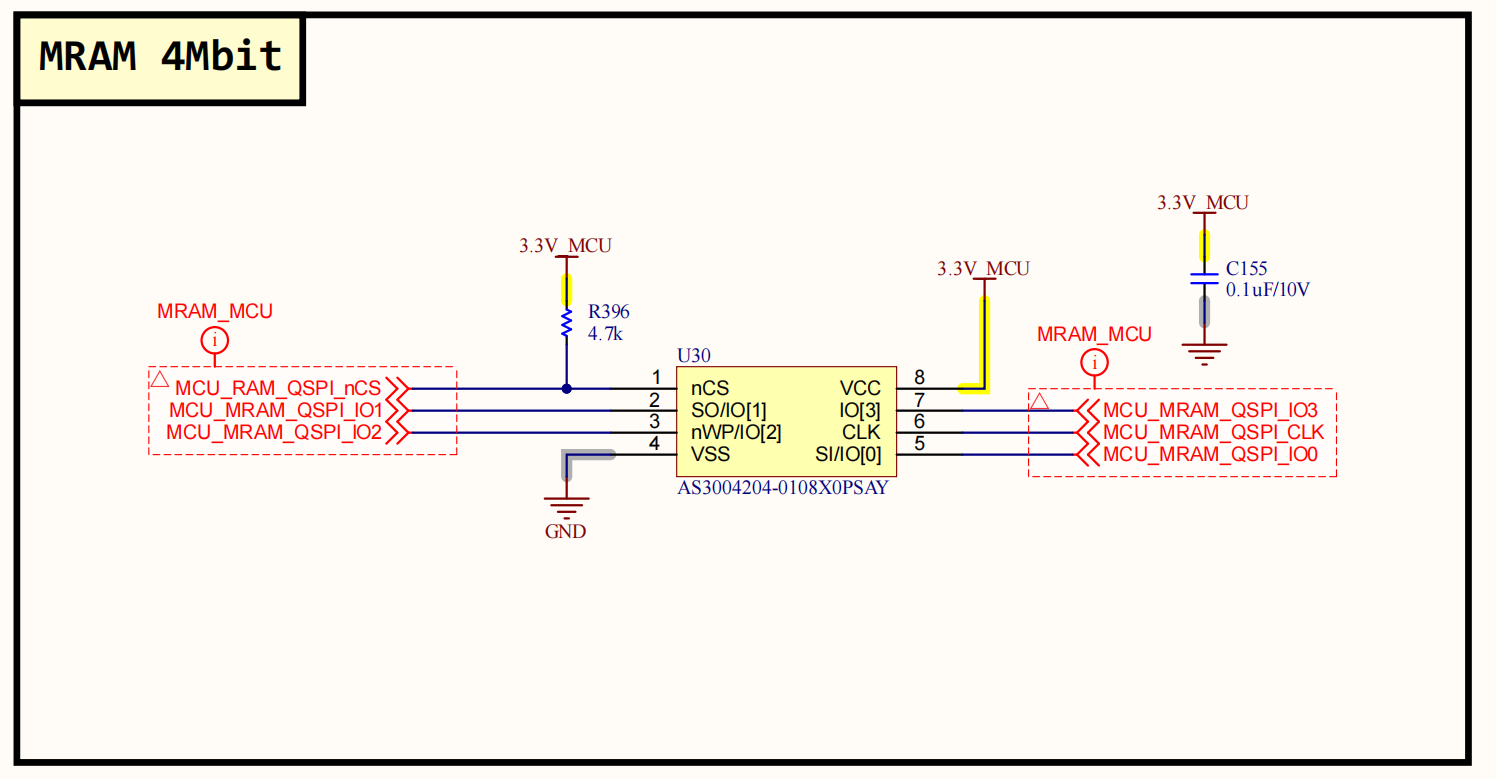
\includegraphics[width=1\textwidth]{picture/exp/mram-mcu.png}
    \\caption{Sơ đồ nguyên lí khối MRAM kết nối MCU}
    \label{fig:exp-sche-mram-mcu}
\end{figure}

\begin{figure}[H]
    \centering
    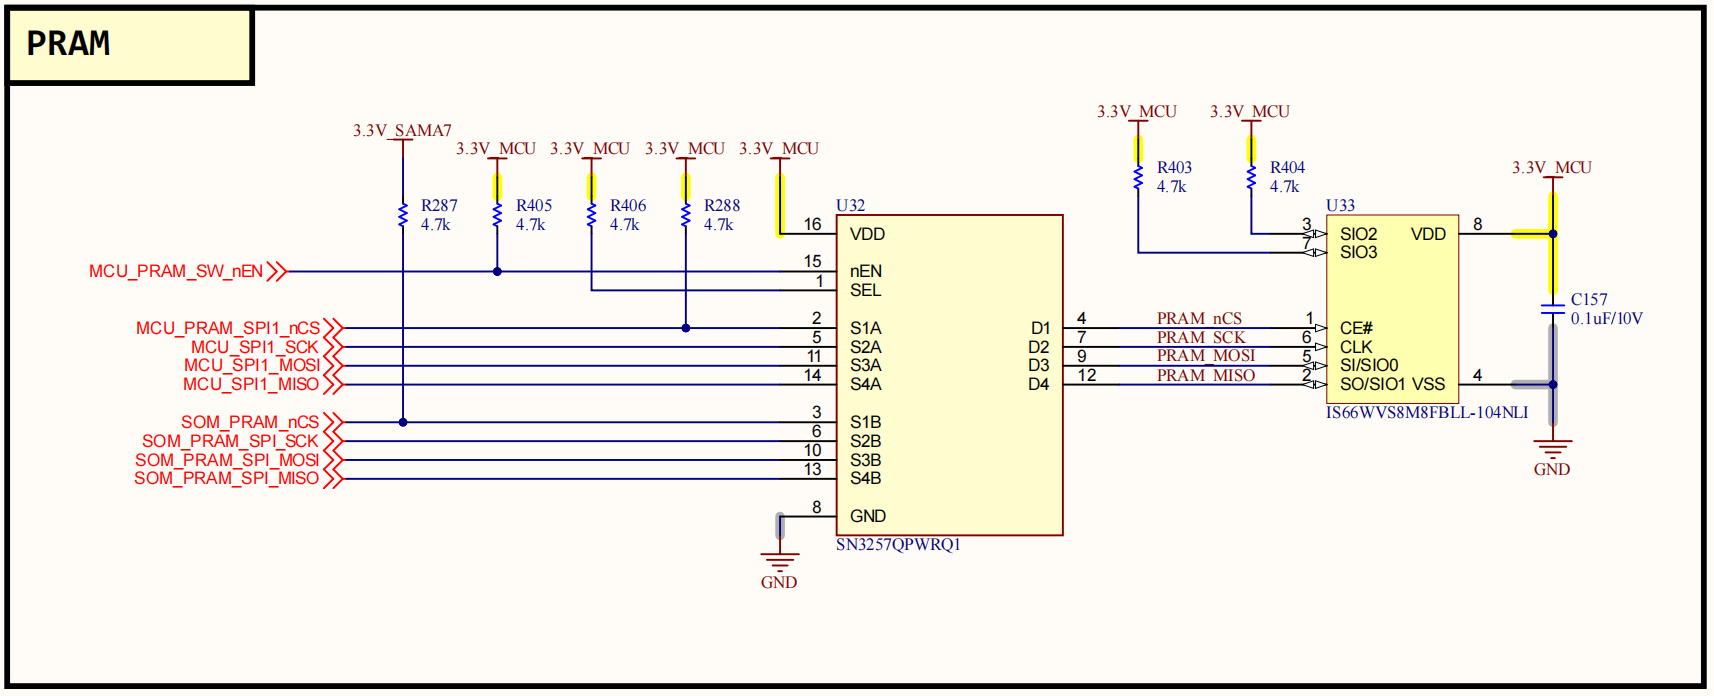
\includegraphics[width=1\textwidth]{picture/exp/pram.png}
    \\caption{Sơ đồ nguyên lí khối PRAM}
    \label{fig:exp-sche-pram}
\end{figure}

Tổng quan chung về các IC RAM được dùng trong thiết kế, bên cạnh RAM DDR3 cho MPU, trên board EXP còn sử dụng thêm 3 IC RAM khác là MRAM, PRAM và FRAM. Bảng \ref{tab:so-sanh-ram} trình bày so sánh chi tiết các đặc tính của ba loại bộ nhớ này:

\begin{table}[H]
    \centering
    \caption{So sánh đặc tính MRAM, PRAM và FRAM}
    \label{tab:so-sanh-ram}
    \begin{tabularx}{\textwidth}{|X|>{\centering\arraybackslash}X|>{\centering\arraybackslash}X|>{\centering\arraybackslash}X|}
    \hline
    \textbf{} & \textbf{MRAM} & \textbf{PRAM} & \textbf{FRAM} \\
    \hline
    Nguyên lí hoạt động & Sử dụng hiệu ứng từ trở, lưu dữ liệu bằng hướng từ hóa của các lớp từ tính & Thay đổi pha vật liệu chalcogenide giữa trạng thái tinh thể và vô định hình, sử dụng nhiệt để chuyển pha & Sử dụng phân cực điện (polarization) của tinh thể ferroelectric để lưu trữ dữ liệu \\
    \hline
    Tốc độ ghi/đọc & Nhanh (sub-nanosecond), tương tự SRAM & Trung bình ($\sim 1$ µs), có thể chậm khi ghi & Cực nhanh (sub-nanosecond), nhanh nhất trong ba \\
    \hline
    Độ bền (chu kỳ ghi) & Rất cao ($\geq 10^{15}$ cycles) & Thấp hơn ($\sim 10^{6}$ - $10^{7}$ cycles) & Rất cao ($\geq 10^{15}$ cycles) \\
    \hline
    Tiêu thụ điện năng & Thấp, chỉ tiêu thụ khi đọc/ghi & Cao khi ghi (do cần nhiệt để thay đổi pha) & Cực thấp, không cần refresh như DRAM \\
    \hline
    Mật độ lưu trữ & Thấp hơn flash & Cao, lớn hơn MRAM/FRAM & Thấp nhất trong ba loại \\
    \hline
    Bay hơi khi mất điện & Không (non-volatile), dữ liệu được giữ nguyên & Không (non-volatile), dữ liệu được giữ nguyên & Không (non-volatile), dữ liệu được giữ nguyên \\
    \hline
    \end{tabularx}
\end{table}

\begin{figure}[H]
    \centering
    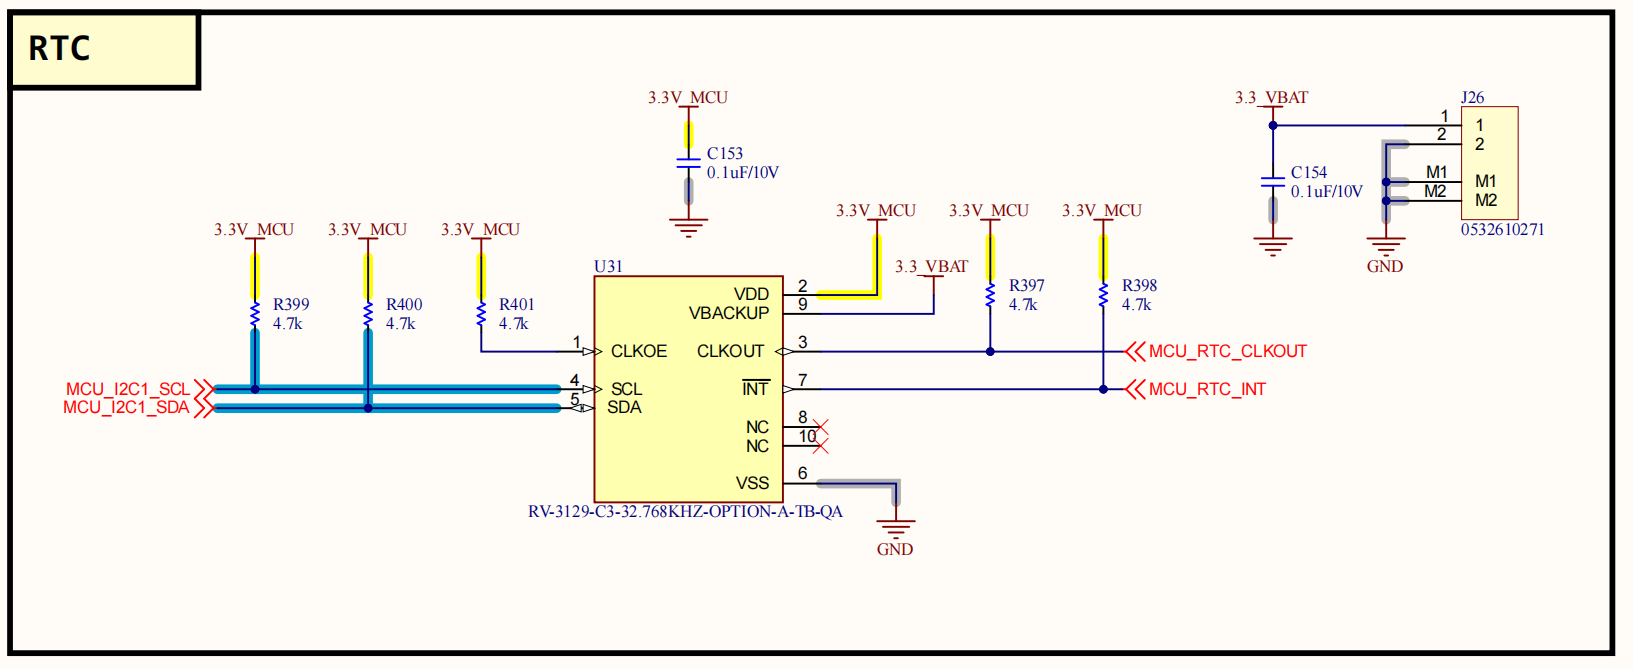
\includegraphics[width=1\textwidth]{picture/exp/rtc.png}
    \\caption{Sơ đồ nguyên lí khối RTC}
    \label{fig:exp-sche-rtc}
\end{figure}

IC RTC sử dụng trong thiết kế là RV-3129-C3-32.768KHZ-OPTION-A-TB-QA của Micro Crystal, một module RTC siêu nhỏ (kích thước 3.2 x 1.5 x 0.8 mm) tích hợp sẵn crystal thạch anh 32.768 kHz với độ chính xác ±1 ppm ở nhiệt độ phòng. IC này giao tiếp qua bus I2C với tốc độ lên đến 400 kHz, hỗ trợ các tính năng như alarm programmable, timer countdown, event detection, và clock output. Ưu điểm chính bao gồm tiêu thụ cực thấp (chỉ 0.045 µA ở chế độ standby), dải nhiệt độ rộng (-40°C đến +85°C), độ tin cậy cao với tuổi thọ >10 năm, và không cần linh kiện ngoài như crystal rời, giúp đơn giản hóa thiết kế PCB.

Các chân PIN của RV-3129 được tối ưu cho ứng dụng low-power: chân SDA và SCL là các chân I2C data và clock, hoạt động open-drain nên bắt buộc phải kéo lên nguồn (pull-up) để đạt mức logic cao; chân INT là chân ngắt output, cũng open-drain nên cần pull-up nếu sử dụng để phát tín hiệu ngắt cho MCU; chân CLKOUT là clock output CMOS push-pull, có thể thả nổi nếu không dùng; chân VBAT là nguồn backup (1.2-5.5V), cần nối pin lithium hoặc tụ để duy trì thời gian khi mất nguồn chính; chân VCC là nguồn hoạt động chính (1.2-5.5V), và GND là đất. Các chân khác như OSCI/OSCO không có vì crystal đã tích hợp.

Trong sơ đồ thiết kế, SDA và SCL được kéo lên 3.3V qua điện trở 4.7 kΩ để đảm bảo tốc độ I2C ổn định và giảm nhiễu trên bus; VBAT nối trực tiếp đến pin backup 3V để bảo toàn thời gian; VCC nối từ nguồn 3.3V của hệ thống; chân INT được kéo lên 3.3V qua 4.7 kΩ để chuẩn bị tín hiệu ngắt nếu kích hoạt alarm; CLKOUT được thả nổi vì không sử dụng trong thiết kế này; GND nối đất chung. Giá trị pull-up 4.7 kΩ được chọn theo khuyến nghị của datasheet để cân bằng giữa tốc độ truyền và tiêu thụ dòng, đảm bảo bus I2C hoạt động ổn định ở 400 kHz mà không gây nhiễu.

\begin{figure}[H]
    \centering
    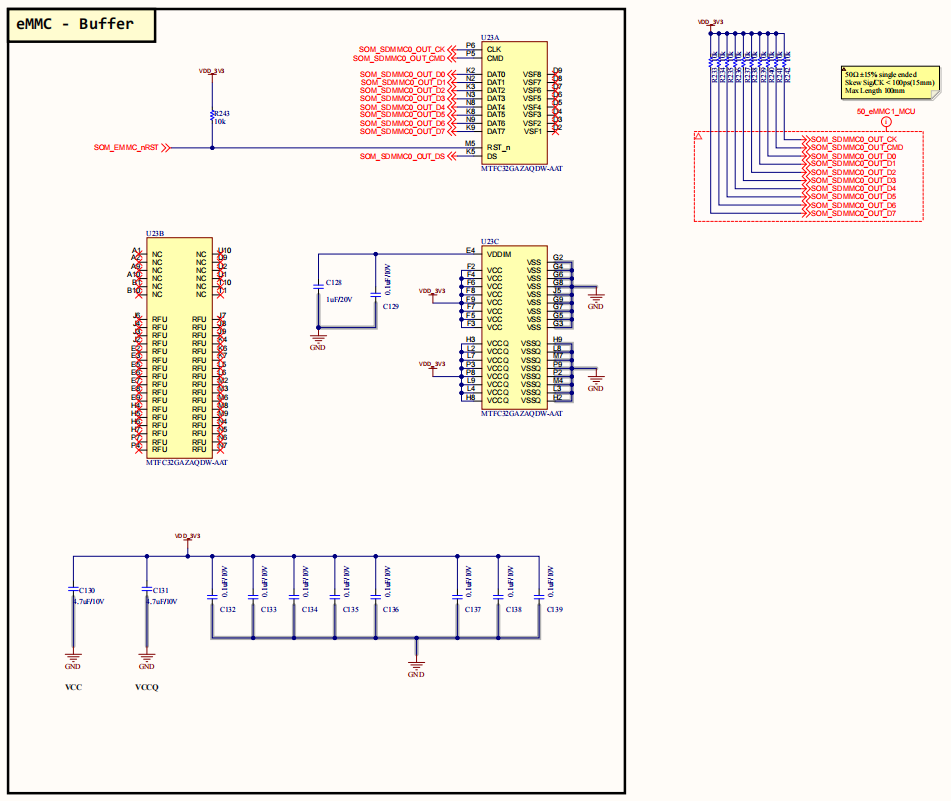
\includegraphics[width=1\textwidth]{picture/exp/khoi-emmc.png}
    \\caption{Sơ đồ nguyên lí khối eMMC}
    \label{fig:exp-sche-khoi-emmc}
\end{figure}

IC eMMC sử dụng trong thiết kế là MTFC32GAZAQDW-AAT của Micron Technology, một module bộ nhớ embedded multimedia card (eMMC) dung lượng 32GB theo chuẩn JEDEC eMMC 5.1. IC này tích hợp NAND flash và MMC controller, hỗ trợ giao tiếp MMC protocol với tốc độ đọc lên đến 250 MB/s và ghi 90 MB/s, cùng chế độ boot trực tiếp từ eMMC. Chức năng chính của eMMC là phục vụ vai trò lưu trữ chính cho firmware, hệ điều hành và dữ liệu dài hạn trong hệ thống nhúng, cho phép boot trực tiếp và quản lý dữ liệu ổn định. Ưu điểm chính bao gồm dung lượng lớn với độ tin cậy cao (ECC tích hợp, wear leveling), tiêu thụ năng lượng thấp (chế độ sleep \textless 1mA), tương thích rộng với các host processor, và không cần driver phức tạp, giúp đơn giản hóa việc lưu trữ firmware và dữ liệu dài hạn trong hệ thống nhúng.

Các chân của MTFC32GAZAQDW-AAT tuân theo chuẩn eMMC: CMD là đường lệnh và DAT0-DAT7 là các đường dữ liệu, cần điện trở kéo lên VCCQ theo khuyến nghị để bảo đảm mức logic ổn định (đặc biệt trong giai đoạn khởi tạo bus); CLK là xung clock từ host nên không cần pull-up; RST\_n là ngõ vào reset, thường kéo lên VCCQ để tránh reset ngoài ý muốn; VCC là nguồn lõi (2.7-3.6 V), VCCQ là nguồn I/O (1.65-3.6 V), và GND là mass; các chân NC (no connect) được để hở.

Trong sơ đồ thiết kế, CMD và DAT0-DAT7 được kéo lên 3.3 V (VCCQ) qua điện trở 10 k$\Omega$ để bảo đảm mức logic ổn định cho bus eMMC; CLK nối trực tiếp từ MPU; RST\_n được kéo lên 3.3 V qua điện trở 10 k$\Omega$ để duy trì trạng thái không reset; VCC và VCCQ nối với nguồn 3.3 V của hệ thống. Chân VDDIM là một nút nguồn nội, nối với tụ kéo xuống đất theo đề xuất thiết kế của datasheet. Giá trị pull-up 10 k$\Omega$ được chọn theo khuyến nghị của datasheet để cân bằng giữa tốc độ bus (52 MHz) và tiêu thụ dòng, bảo đảm truyền tín hiệu ổn định.

\begin{figure}[H]
    \centering
    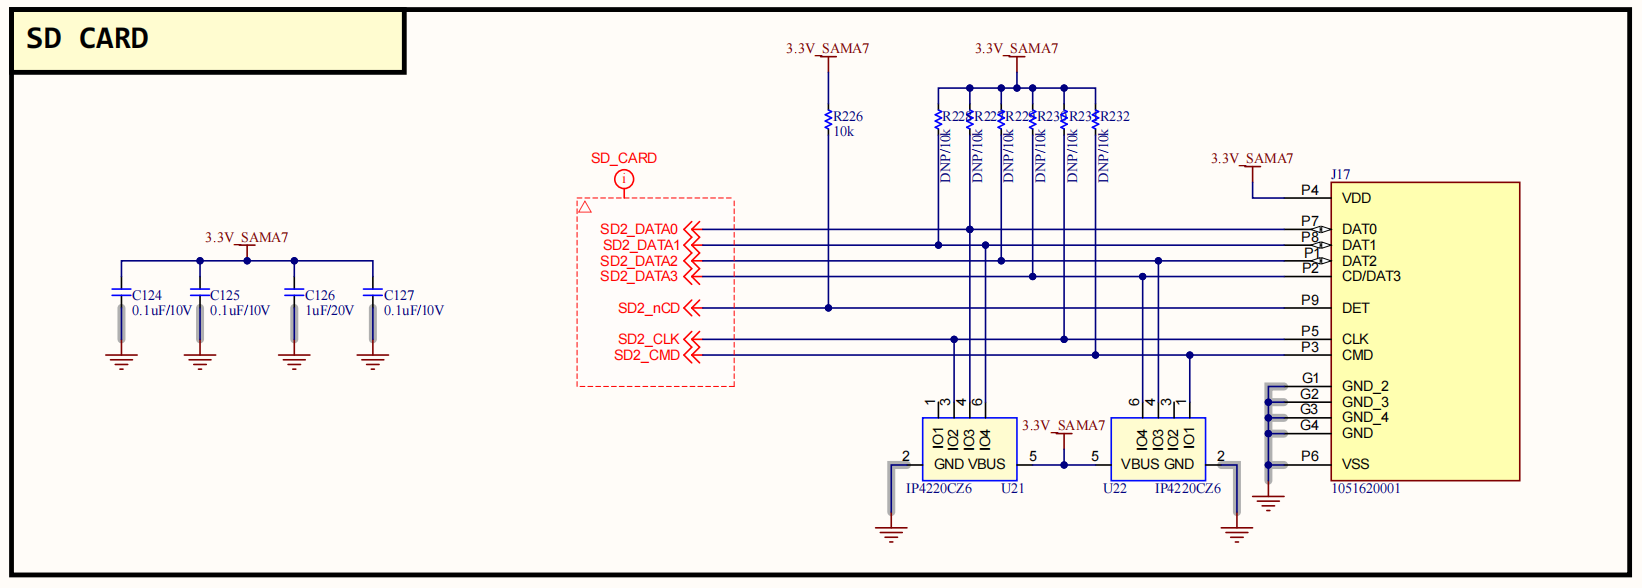
\includegraphics[width=1\textwidth]{picture/exp/sdcard.png}
    \\caption{Sơ đồ nguyên lí khối SD Card}
    \label{fig:exp-sche-sdcard}
\end{figure}

Bên cạnh eMMC là một thẻ nhớ nhúng dùng để boot, còn dùng thêm 1 thẻ SD Card khác để boot các phần mềm cần thiết cho core MPU, cũng sử dụng qua giao thức SDMMC (SDMMC1 với MPU).

\begin{figure}[H]
    \centering
    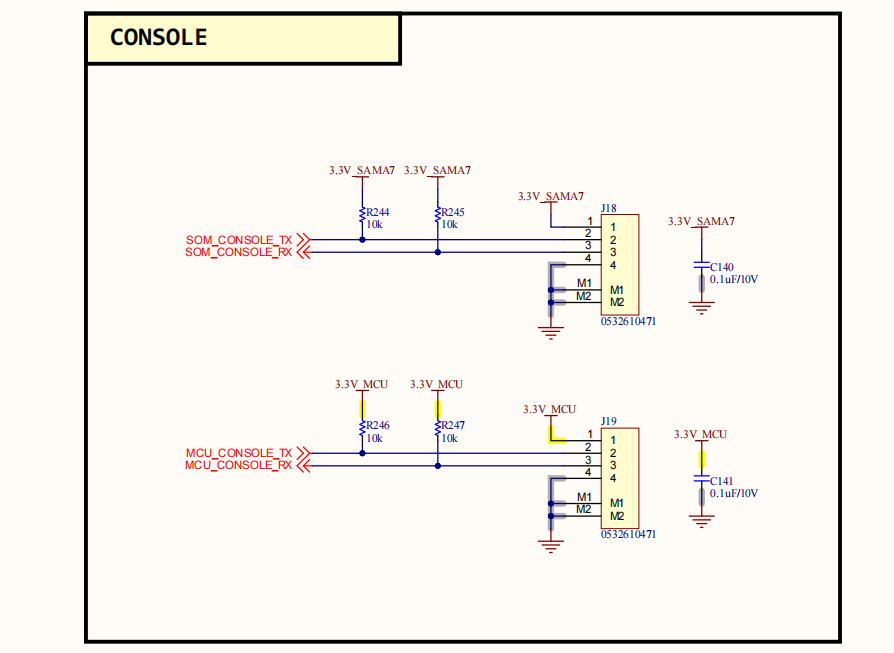
\includegraphics[width=1\textwidth]{picture/exp/khoi-debug.png}
    \\caption{Sơ đồ nguyên lí khối Debug}
    \label{fig:exp-sche-khoi-debug}
\end{figure}

Các connector debug console với giao thức UART để thực hiện quá trình debug trong lúc phát triển firmware.

\begin{figure}[H]
    \centering
    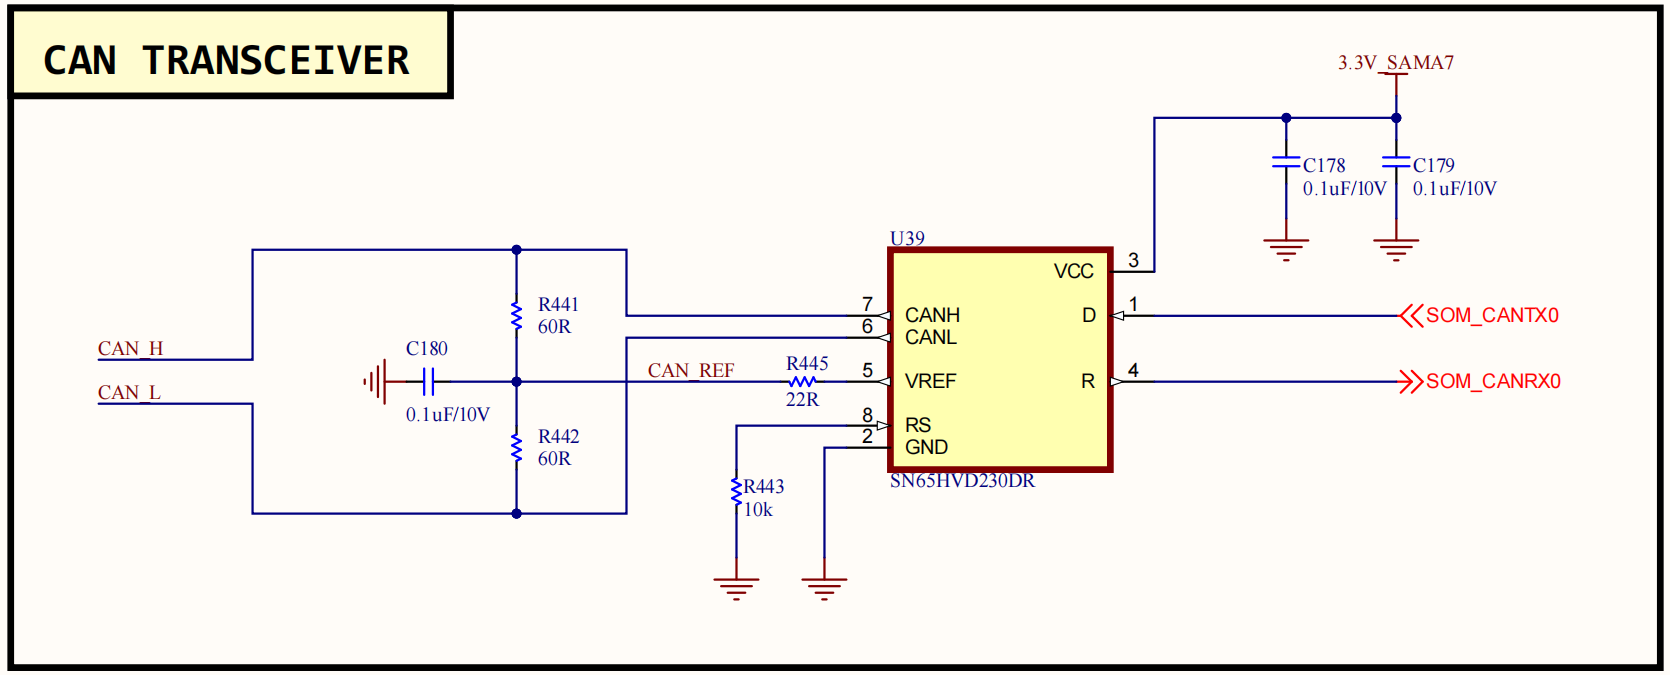
\includegraphics[width=1\textwidth]{picture/exp/CAN-transceiver.png}
    \\caption{Sơ đồ nguyên lí khối CAN transceiver}
    \label{fig:exp-sche-can-transceiver}
\end{figure}

Thiết kế sửa dụng IC CAN TRANSCEIVER SN65HVD230DR, để chuyển đổi tín hiệu CAN ở lớp giao thức vật lý, chuyển đổi từ tín hiệu single-end sang diffental pair và ngược lại. Đối với CAN TRANSCEIVER có vai trò là điểm ở cuối đường dây bus CAN, phải cần thêm một điện trở phối hợp trở kháng cuối đường dây thường là 120R đối với đường truyền CAN.

\begin{figure}[H]
    \centering
    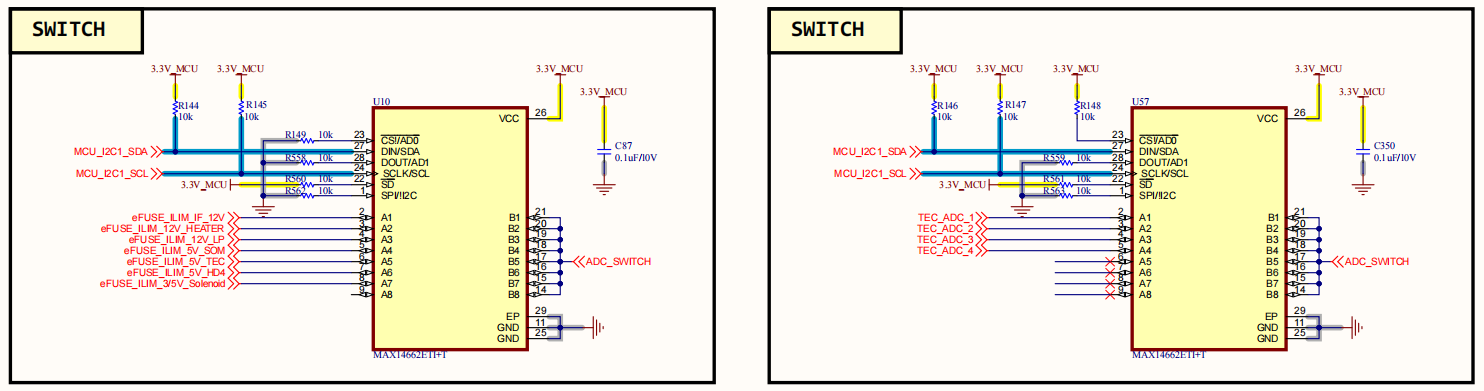
\includegraphics[width=1\textwidth]{picture/exp/sw-usb.png}
    \\caption{Sơ đồ nguyên lí khối chuyển mạch USB}
    \label{fig:exp-sche-sw-usb}
\end{figure}


Trong thiết kế, MAX14662ETI+T (Maxim Integrated/Analog Devices) được sử dụng như một switch với nhiều ngõ vào và một ngõ ra, một ngõ ra được đọc về MCU và MCU sẽ chọn tín hiệu đọc về thông qua I2C. Do hạn chế về mặt số lượng chân ADC và các tín hiệu ADC sẽ được đọc tùy ý nên dùng switch sẽ đáp ứng được cho việc đọc được nhiều tín hiệu ADC và đáp ứng được việc không bắt buộc đọc cùng lúc.

Các ưu điểm chính của MAX14662ETI+T gồm: dải nguồn đơn rộng từ 1.6~V đến 5.5~V; khả năng truyền tín hiệu analog đến $\pm 5.5$~V độc lập với mức nguồn nuôi (\textit{Beyond-the-Rails}); điện trở dẫn thấp (R\textsubscript{ON} điển hình khoảng 0.425~$\Omega$); độ méo thấp; hỗ trợ băng thông cao; và các chân tín hiệu A\_x/B\_x có mức bảo vệ ESD cao, phù hợp khi làm việc với các cổng giao tiếp ngoài.

\begin{figure}[H]
    \centering
    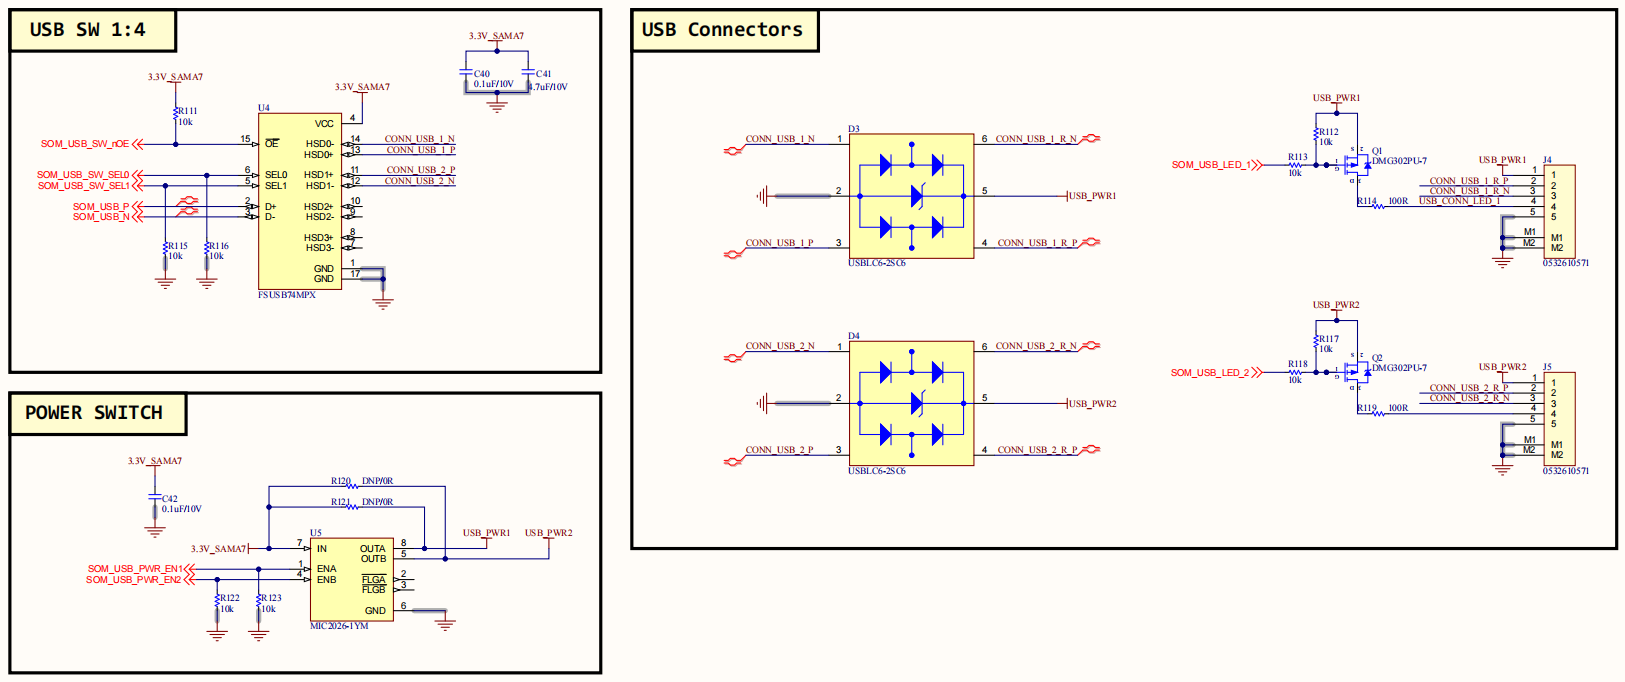
\includegraphics[width=1\textwidth]{picture/exp/usb_host_only.png}
    \\caption{Sơ đồ nguyên lí khối USB host only}
    \label{fig:exp-sche-sw-usb-connector}
\end{figure}

Do hạn chế về số lượng USB trên MPU, theo yêu cầu thiết kế cần 2 connector USB host only nên phải dùng 1 usb switch (IC FSUSB74MPX) có ngõ vào từ USB\_C (host only của MPU) và 2 ngõ ra cho 2 connector USB.

Bên cạnh switch cho tín hiệu USB, dùng thêm một IC switch nguồn để tùy vào khi ta kết nối với connector nào thì ta có thể kiểm soát độc lập nguồn trên connector đó lẫn việc chọn tín hiệu USB. Trong thiết kế dùng IC MIC2026-1YM.

Gần phía connector usb sử dụng 2 IC USBLC6-2SC6 để kẹp mức điện áp an toàn, bảo vệ linh kiện trên mạch khỏi hiện tượng ESD.

\begin{figure}[H]
    \centering
    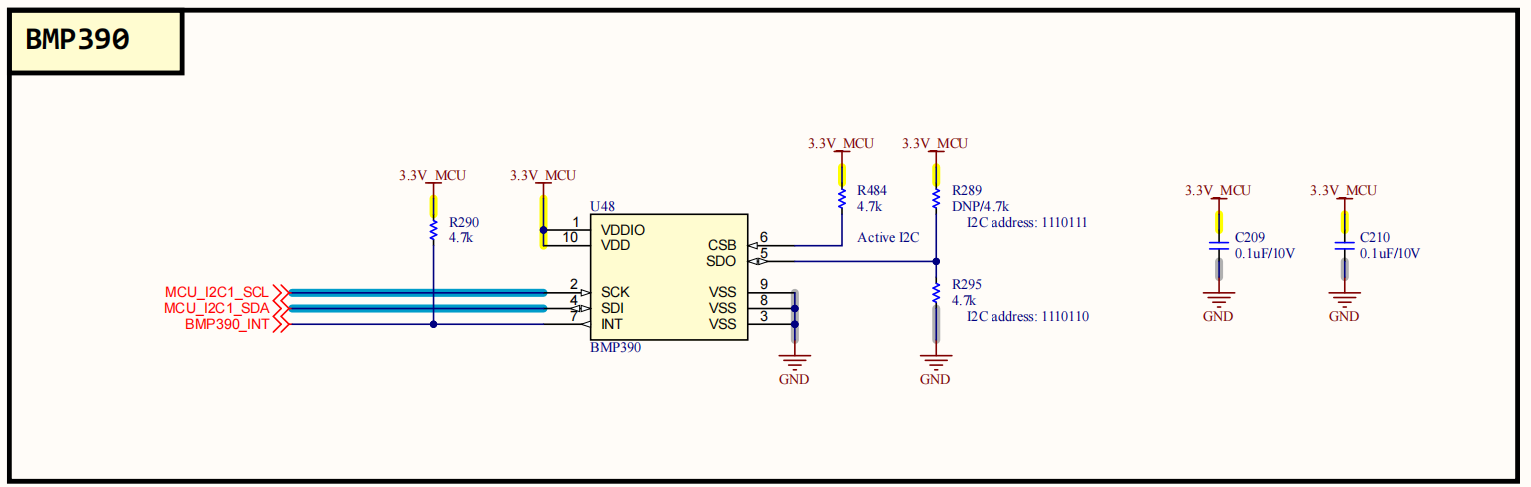
\includegraphics[width=1\textwidth]{picture/exp/bmp390-onboard.png}
    \caption{Schematic cảm biến BMP390 onboard}
    \label{fig:exp-sche-bmp390-onboard}
\end{figure}

\begin{figure}[H]
    \centering
    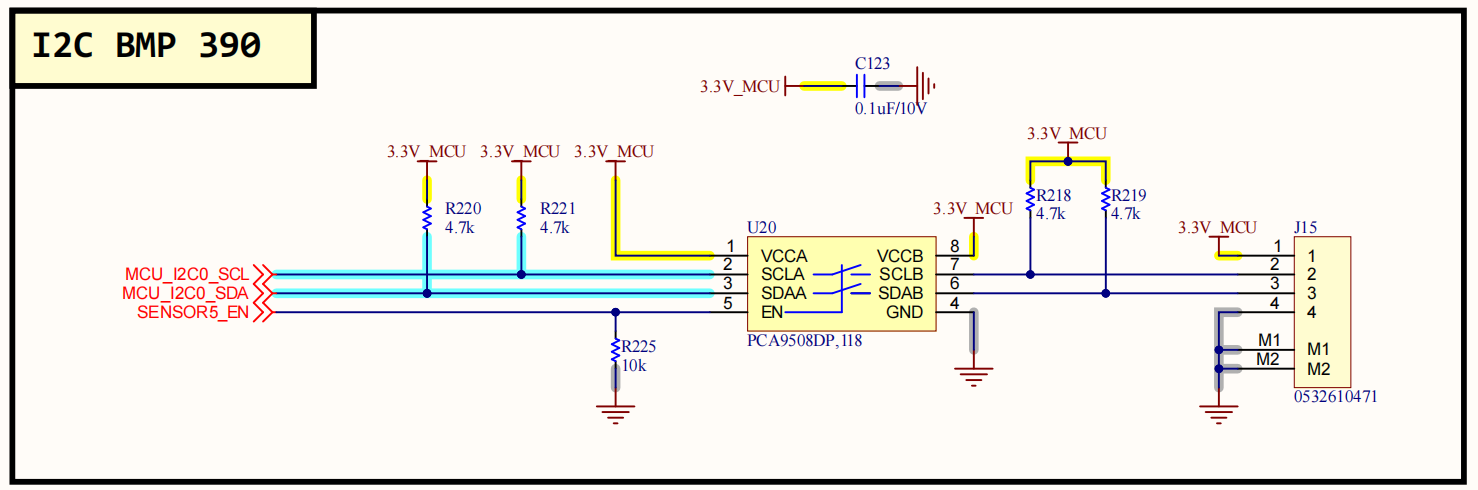
\includegraphics[width=1\textwidth]{picture/exp/bmp390-connector.png}
    \caption{Schematic connector BMP390}
    \label{fig:exp-sche-bmp390-connector}
\end{figure}

Thiết kế sử dụng BMP390 onboard và kết nối ra connector để đo đạc thông số nhiệt độ áp suất trên board và môi trường ngoài board. BMP390 là dòng cảm biến áp suất khí quyển kỹ thuật số hiệu suất cao của Bosch Sensortec, được tối ưu hóa cho các ứng dụng cần độ chính xác cực cao về cao độ. Linh kiện hoạt động trong dải áp suất từ $300$ đến $1250$ hPa với độ sai số tương là $\pm 0.03$ hPa (tương đương sai số độ cao chỉ 25 cm). Với kích thước nhỏ ($2.0 \times 2.0 \times 0.75$ mm³), mức tiêu thụ năng lượng thấp và tích hợp sẵn bộ đệm FIFO 73 khung dữ liệu, BMP390 cho phép giảm tải xử lý cho vi điều khiển trung tâm đồng thời kéo dài thời lượng pin. Cảm biến hỗ trợ hai giao tiếp I2C và SPI, tích hợp sẵn cảm biến nhiệt độ bên trong để bù sai số môi trường.

\begin{figure}[H]
    \centering
    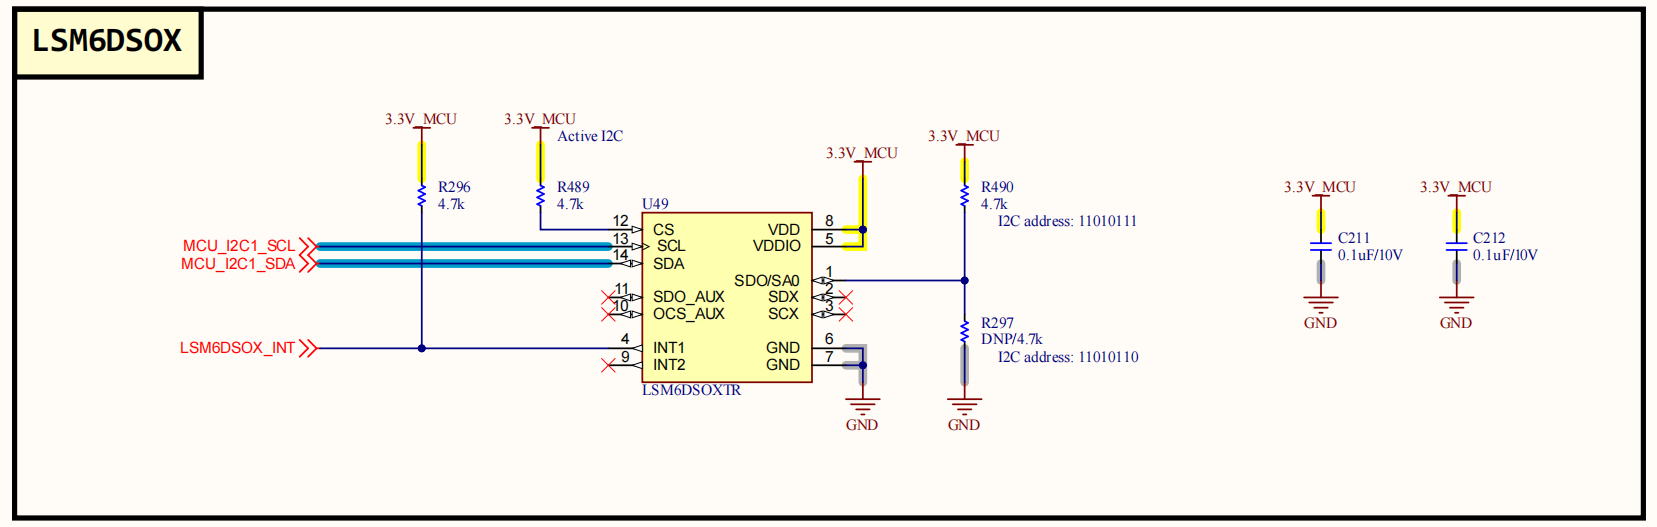
\includegraphics[width=1\textwidth]{picture/exp/cam-bien-gia-toc.png}
    \caption{Schematic cảm biến gia tốc}
    \label{fig:exp-sche-cam-bien-gia-toc}
\end{figure}

LSM6DSOX là cảm biến MEMS 6 trục (gia tốc và con quay hồi chuyển) kỹ thuật số. Thiết bị điều khiển qua giao tiếp I²C/SPI/I3C, xuất dữ liệu 16-bit, tín hiệu ngắt và hỗ trợ OIS chuyên dụng. Ưu điểm là tiêu thụ điện thấp (0.55 mA), tích hợp sẵn Lõi học máy (MLC) và 16 Máy trạng thái (FSM) giúp xử lý thông minh tại biên và giảm tải tối đa cho vi xử lý chính. 

Trong thiết kế đang dùng I2C chung bus I2C dùng cho các IC nội bộ trên board (). IC LSM6DSOX nó sẽ có 2 địa chỉ slave được cấu hình bởi việc kéo lên hoặc kéo xuống ở chân SDO/SA0.

\begin{figure}[H]
    \centering
    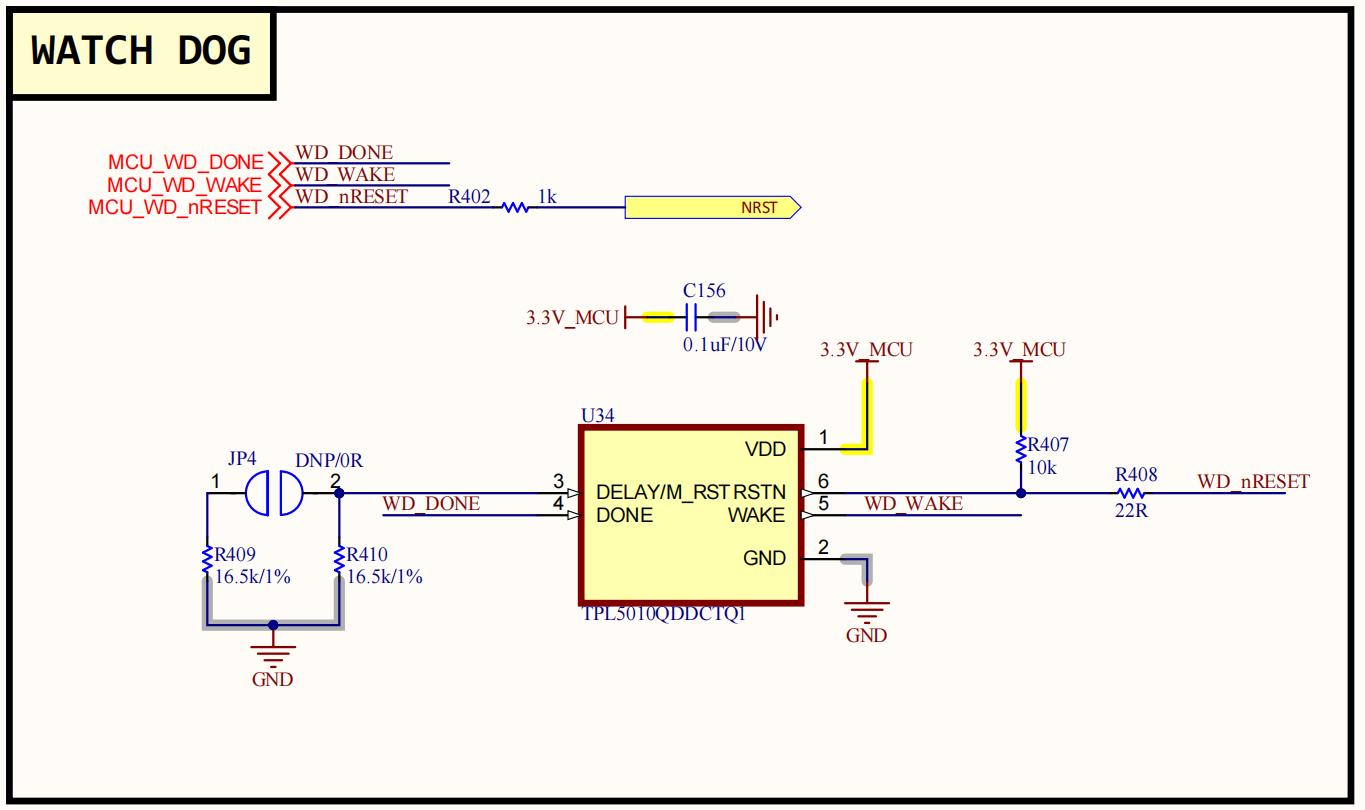
\includegraphics[width=1\textwidth]{picture/exp/watchdog.png}
    \\caption{Sơ đồ nguyên lí khối watchdog}
    \label{fig:exp-sche-watchdog}
\end{figure}

TPL5010-Q1 là bộ định thời hệ thống tiêu thụ năng lượng nano, tích hợp tính năng watchdog, dùng để đánh thức vi điều khiển ($\mu$C) định kỳ trong các ứng dụng chạy pin.

Về nguyên lý hoạt động, IC phát xung WAKE theo chu kỳ xác định (từ 100~ms đến 7200~s), được lập trình thông qua giá trị điện trở ngoài $R_{EXT}$ nối vào chân DELAY/M\_RST. Sau khi nhận lệnh đánh thức, vi điều khiển phải phản hồi bằng tín hiệu DONE cho IC ít nhất 20~ms trước khi chu kỳ đánh thức tiếp theo bắt đầu; nếu IC không nhận được phản hồi này (ví dụ vi điều khiển bị treo hoặc lỗi), IC sẽ kích hoạt chân RSTn để reset hệ thống. Các tín hiệu chính gồm: WAKE (phát xung đánh thức), DONE (nhận phản hồi từ $\mu$C), RSTn (đầu ra reset cực máng hở, yêu cầu điện trở kéo lên), và DELAY/M\_RST (thiết lập thời gian bằng điện trở và hỗ trợ reset thủ công khi được kéo lên mức VDD).

\noindent Để thiết lập khoảng thời gian, điện trở ngoài $R_{EXT}$ được chọn theo công thức sau:
\begin{equation}
R_{EXT}=100\left(\frac{-b+\sqrt{b^2-4a\left(c-100T\right)}}{2a}\right)
\end{equation}

\noindent Trong đó:
\begin{itemize}
    \item $T$ là khoảng thời gian mong muốn, đơn vị giây
    \item $R_{EXT}$ là giá trị điện trở sử dụng, đơn vị $\Omega$
    \item $a, b, c$ là các hệ số phụ thuộc vào dải khoảng thời gian
\end{itemize}

\begin{table}[H]
    \centering
    \caption{Các hệ số cho công thức tính $R_{EXT}$}
    \label{tab:rext-coefficients}
    \begin{tabular}{|c|c|c|c|c|}
        \hline
        \textbf{SET} & \textbf{Dải thời gian $T$ (s)} & \textbf{a} & \textbf{b} & \textbf{c} \\
        \hline
        1 & $1 < T \leq 5$ & 0.2253 & -20.7654 & 570.5679 \\
        \hline
        2 & $5 < T \leq 10$ & -0.1284 & 46.9861 & -2651.8889 \\
        \hline
        3 & $10 < T \leq 100$ & 0.1972 & -19.3450 & 692.1201 \\
        \hline
        4 & $100 < T \leq 1000$ & 0.2617 & -56.2407 & 5957.7934 \\
        \hline
        5 & $T > 1000$ & 0.3177 & -136.2571 & 34522.4680 \\
        \hline
    \end{tabular}
\end{table}

Tùy thuộc vào thời gian thiết lập từ đó chọn các tham số a, b, c và tính lại giá trị $R_{EXT}$ cần cho thiết kế.

\begin{figure}[H]
    \centering
    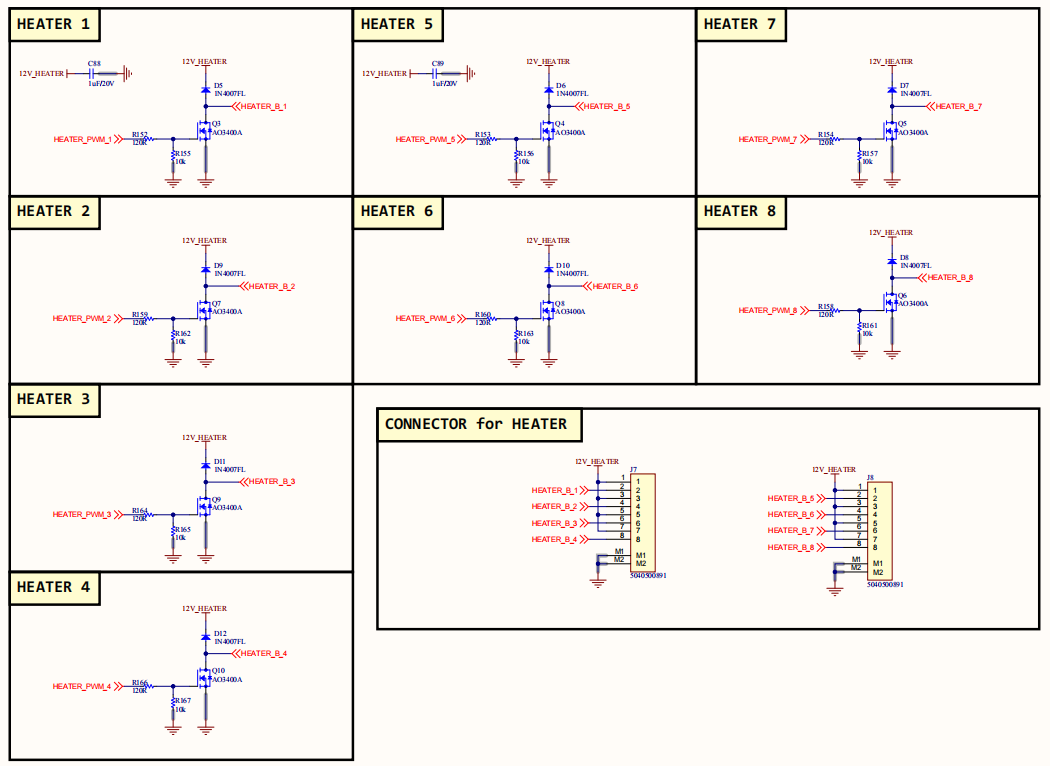
\includegraphics[width=1\textwidth]{picture/exp/khoi-heater.png}
    \\caption{Sơ đồ nguyên lí khối Heater}
    \label{fig:exp-sche-khoi-heater}
\end{figure}

Khối heater bao gồm 8 heater được điều khiển bởi tín hiệu PWM thông qua N\_MOSFER và kết nối ra connector heater.

\begin{figure}[H]
    \centering
    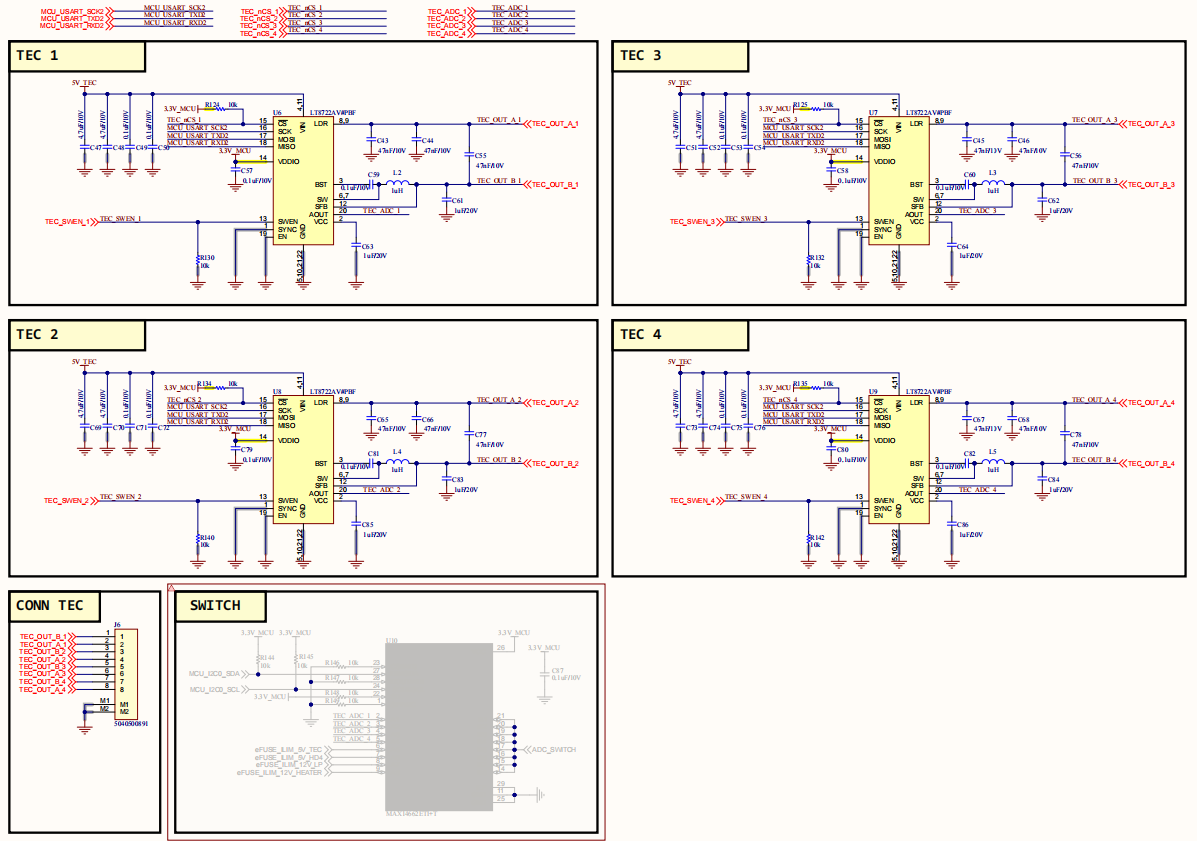
\includegraphics[width=1\textwidth]{picture/exp/khoi-tec.png}
    \\caption{Sơ đồ nguyên lí khối TEC}
    \label{fig:exp-sche-khoi-tec}
\end{figure}
Khối TEC điều khiển phần tử nhiệt điện (làm nóng/làm lạnh), giúp duy trì môi trường nhiệt mục tiêu cho buồng đo.

Trong thiết kế sử dụng IC LT8722 là bộ điều khiển full bridge DC/DC, chuyên dùng để lái bộ làm mát nhiệt điện (TEC) và các hệ thống quang học với công suất lên đến ±54W. Một phía tải được điều khiển bằng tầng PWM buck và phía còn lại bằng tầng tuyến tính, cho phép điều khiển dòng điện hai chiều chính xác mà chỉ cần một cuộn cảm. IC giao tiếp thông SPI 10MHz để cấu hình điện áp (DAC 25-bit) và giới hạn dòng điện, đồng thời xuất tín hiệu giám sát hệ thống (VIN, VOUT, nhiệt độ) qua chân AOUT. Trong thiết kế này, do giới hạn về số lượng ngoại vi nên SPI được dùng thay thế bởi USART.

Trong thiết kế này, LT8722 đóng vai trò là bộ điều khiển dòng điện hai chiều cho module TEC dựa trên cấu trúc Full-bridge tích hợp. IC sử dụng cơ chế điều khiển dòng điện (Constant Current) thay vì điều khiển điện áp, giúp duy trì dòng định mức qua tải bất chấp sự biến đổi nội trở của vật liệu bán dẫn theo nhiệt độ. DAC 25-bit cho phép thiết lập điểm vận hành (setpoint) và điều chỉnh cường độ dòng điện với bước nhảy nhỏ, đảm bảo độ phân giải trong việc kiểm soát nhiệt độ. Tầng công suất kết hợp giữa PWM buck và tầng tuyến tính cho phép thay đổi chiều dòng điện liên tục giữa chế độ làm lạnh và chế độ sưởi ấm mà không bị gián đoạn tại điểm dòng bằng không. Ngoài ra, các tính năng giám sát hệ thống qua giao tiếp SPI và chân AOUT cung cấp dữ liệu về điện áp đầu vào, đầu ra và nhiệt độ thực tế của IC. Do hạn chế về số lượng chân ngoại vi trên vi điều khiển, SPI được sử dụng thay thế bởi USART.

\begin{figure}[H]
    \centering
    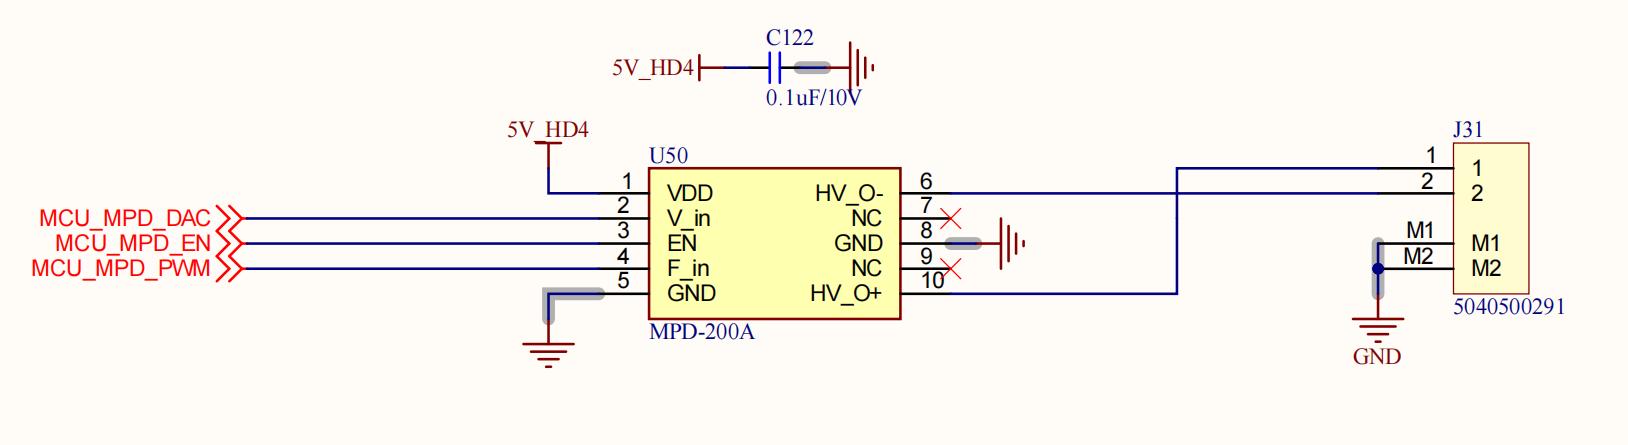
\includegraphics[width=1\textwidth]{picture/exp/mpd200a.png}
    \\caption{Sơ đồ nguyên lí khối MPD200A}
    \label{fig:exp-sche-mpd200a}
\end{figure}
Theo schematic của board EXP, khối MPD200A là phần đại diện cho module nguồn HV mà MCU tương tác thông qua các tín hiệu DAC, EN và PWM; trong đó EN dùng để cho phép/khóa hoạt động, còn DAC/PWM dùng để đặt mức hoặc điều chế công suất theo yêu cầu điều khiển. Ngõ ra của khối là cặp cao áp HV\_O+ và HV\_O- đưa ra connector tới tải.

Đối chiếu với datasheet MPD-200, các chân điều khiển chuẩn của module chủ yếu ở mức hệ nguồn (remote on/off, power good, remote sense). Vì vậy, các tín hiệu DAC, EN, PWM trong schematic này được hiểu là giao diện điều khiển ở cấp hệ thống của board mạch (hoặc qua mạch ghép trung gian), dùng để MCU điều khiển nhánh HV một cách chủ động và an toàn.

\begin{figure}[H]
    \centering
    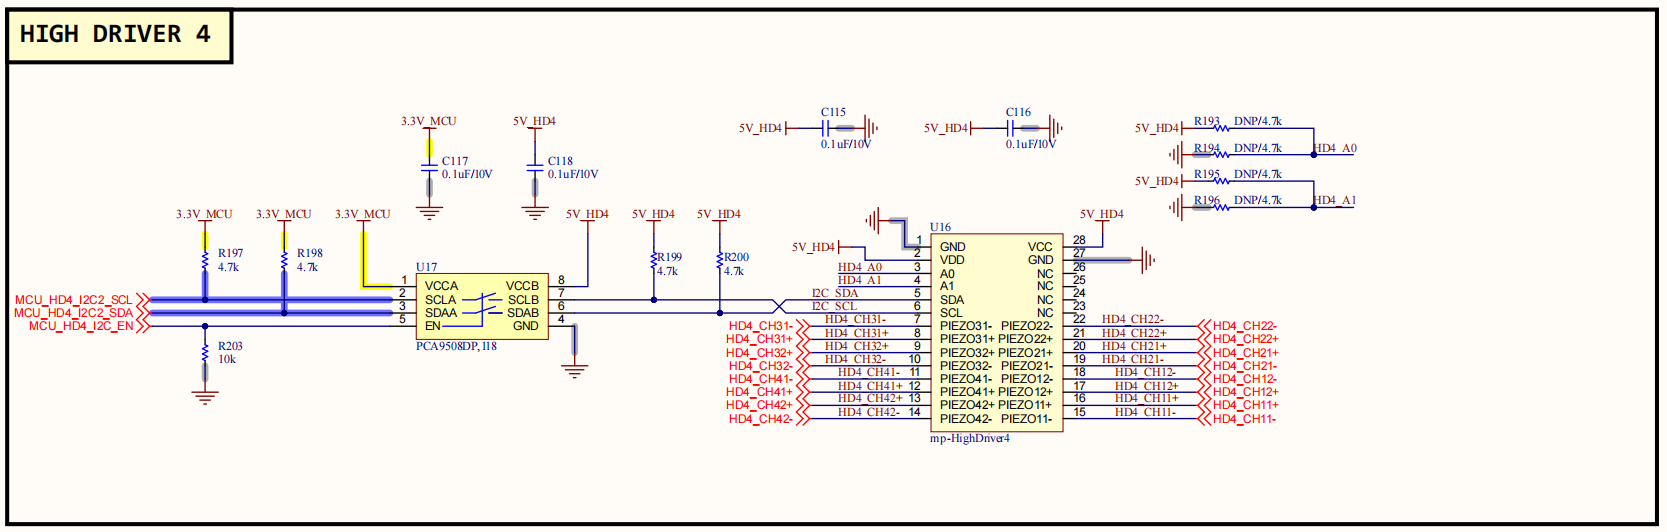
\includegraphics[width=1\textwidth]{picture/exp/driver-hd4.png}
    \\caption{Sơ đồ nguyên lí khối driver HD4}
    \label{fig:exp-sche-driver-hd4}
\end{figure}
Module này đóng vai trò là một bộ chuyển đổi DC-AC điện áp cao. Nó lấy nguồn điện một chiều (DC) thấp từ pin hoặc hệ thống và chuyển đổi thành tín hiệu xoay chiều (AC) có biên độ lớn để kích hoạt các màng loa áp điện (piezo membrane) bên trong máy bơm mp6. Đặc biệt, phiên bản mp-Highdriver4 có khả năng lái cùng lúc lên đến 4 máy bơm mp6 một cách độc lập. Giao tiếp I2C để tùy chỉnh tần số, biên độ điện áp, dạng sóng.
\begin{figure}[H]
    \centering
    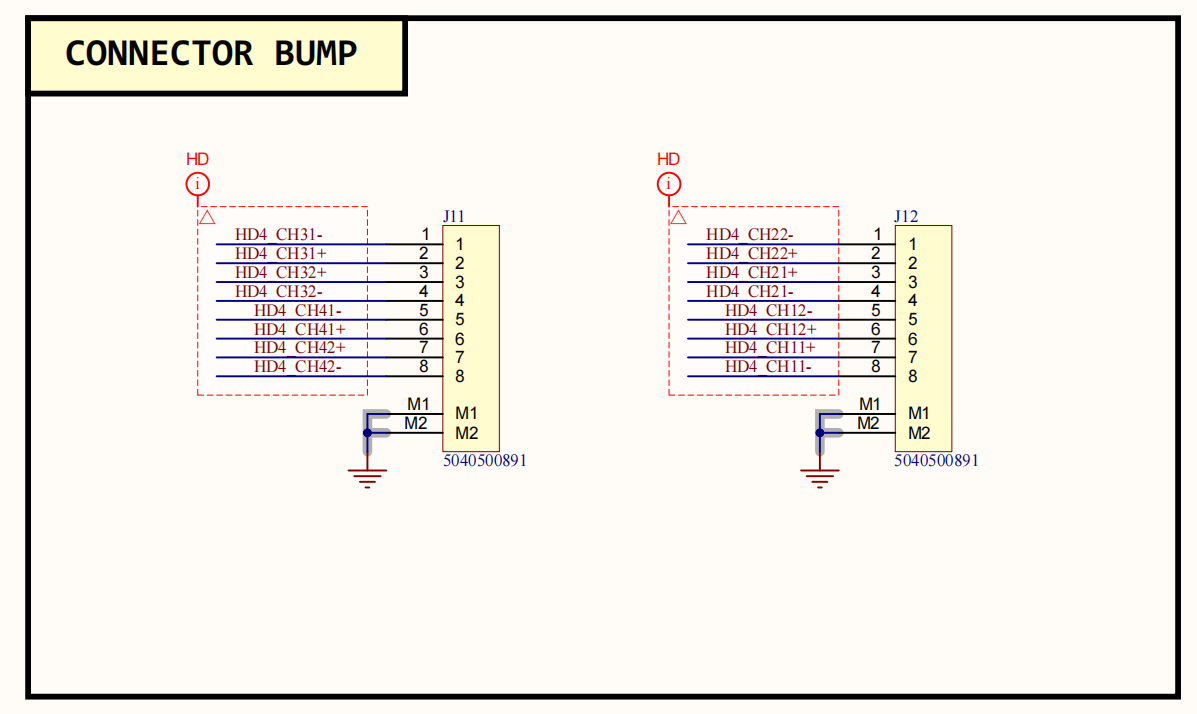
\includegraphics[width=0.7\textwidth]{picture/exp/connector-hd4.png}
    \caption{Schematic connector HD4}
    \label{fig:exp-sche-connector-hd4}
\end{figure}

Các tín hiệu được lái từ IC mp-Highdriver4 sẽ được kết nối ra connector kết nối với các máy bơm màng piezo.

\begin{figure}[H]
    \centering
    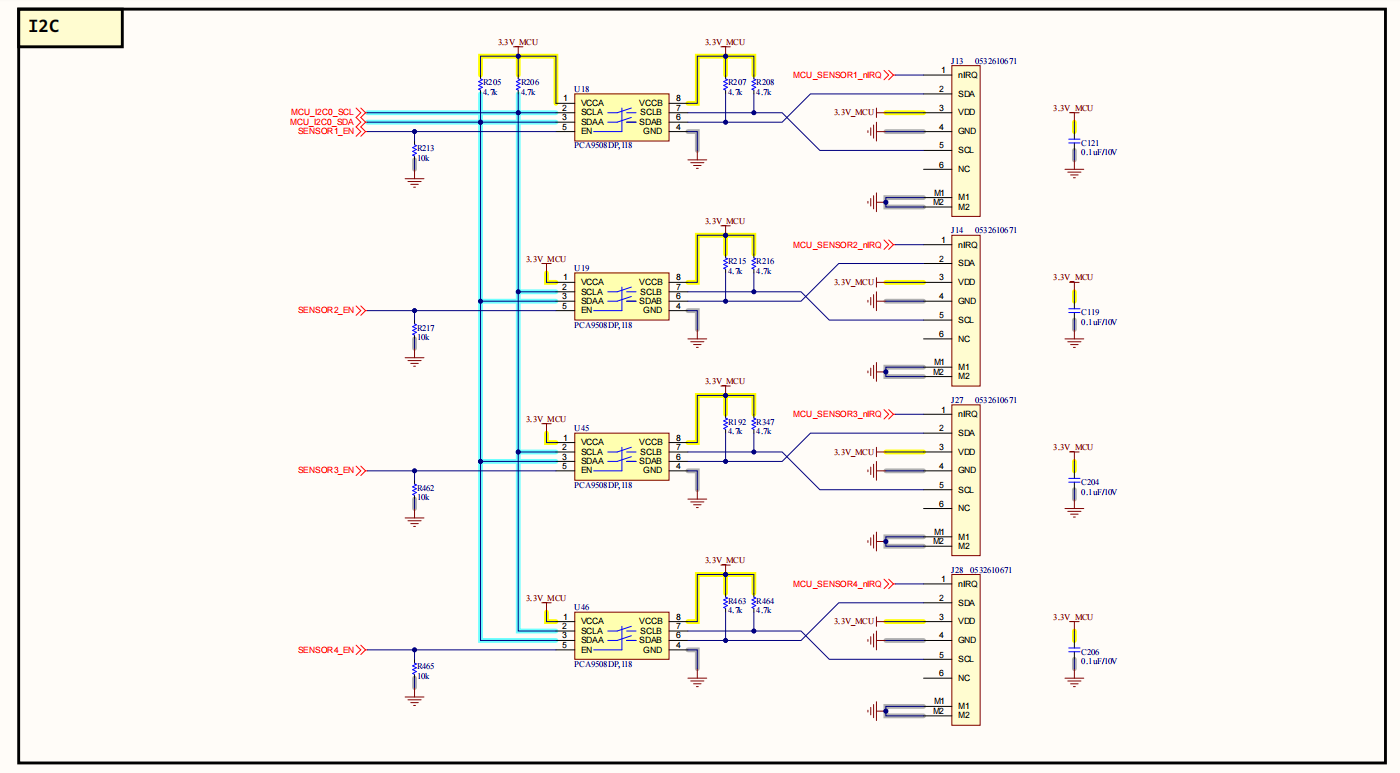
\includegraphics[width=1\textwidth]{picture/exp/flow-ic.png}
    \\caption{Sơ đồ nguyên lí khối giao tiếp flow sensor}
    \label{fig:exp-sche-flow-ic}
\end{figure}

Cảm biến lưu lượng (flow sensor) là thiết bị dùng để đo tốc độ hoặc khối lượng của chất lỏng hoặc khí chảy qua một ống dẫn. IC được kéo ra connector và được khiển bởi tín hiệu I2C. IC flow kết hợp với IC bump để tạo ra một hệ phản hồi kín, một thành phần đóng vai trò điều khiển công suất bơm lưu và một thành phần đóng vai trò theo dõi lưu lượng bơm để trả về dữ liệu cho MCU xử lí và cân chỉnh IC bump cũng như lưu trữ thông tin bơm. 

\begin{figure}[H]
    \centering
    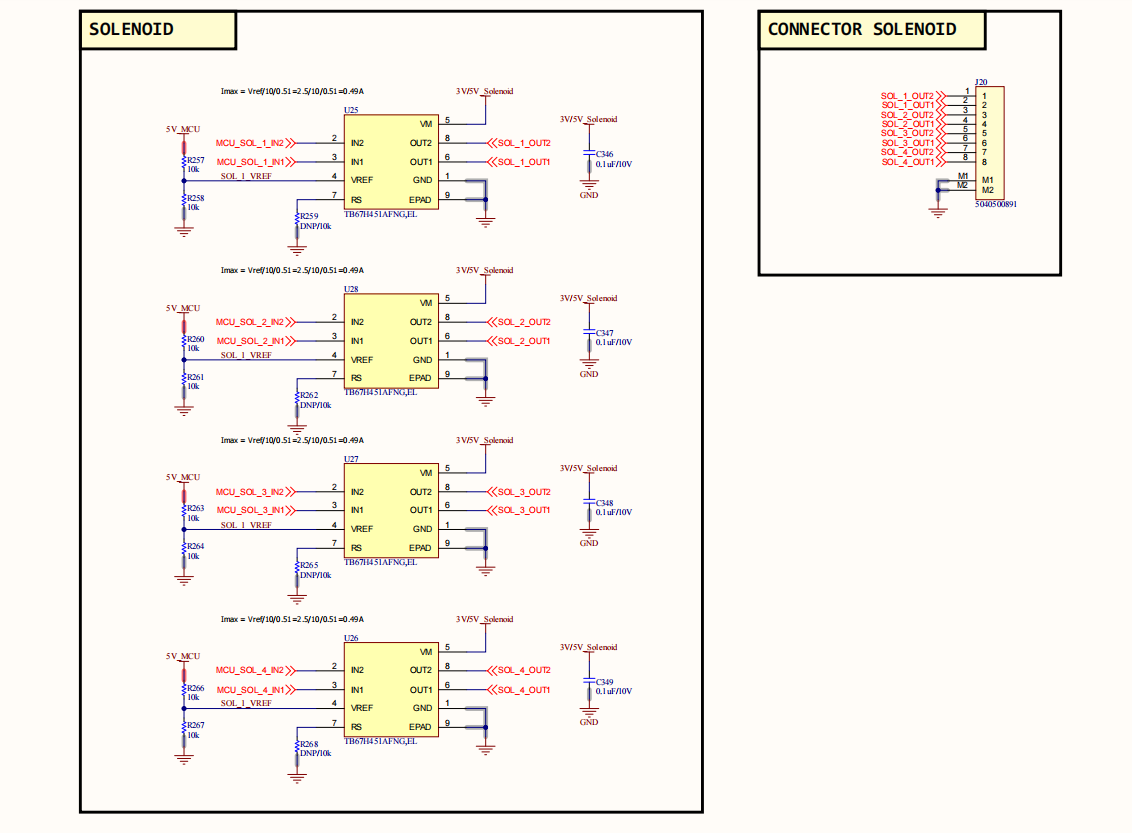
\includegraphics[width=1\textwidth]{picture/exp/solenoid-ic.png}
    \\caption{Sơ đồ nguyên lí khối điều khiển solenoid thứ nhất}
    \label{fig:exp-sche-solenoid-ic}
\end{figure}

TB67H451AFNG là một vi mạch điều khiển động cơ DC chổi than (brushed motor driver) kiểu băm xung PWM, cho phép chịu được điện áp lên tới 50 V và dòng điện tối đa 3.5A. Khả năng lái dòng điện không đổi bằng PWM hoặc lái PWM trực tiếp. Tích hợp các chức năng phát hiện lỗi: Ngắt quá nhiệt (TSD), phát hiện quá dòng (ISD) và khóa dưới điện áp (UVLO). mạch sử dụng một cầu H (H-Bridge) tích hợp để điều khiển dòng điện đi qua tải. Tùy thuộc vào trạng thái của IN1 và IN2, vi mạch sẽ hoạt động theo 4 chế độ.

Tín hiệu input là IN1 và IN2 dùng để làm tổ hợp lựa chọn chế độ hoạt động để tạo ngõ ra.

VREF là chân để thiết lập giá trị dòng điện đầu ra cho động cơ.

\begin{equation}
I_{\mathrm{out(max)}} = V_{\mathrm{ref(gain)}} \times \frac{V_{\mathrm{ref}}}{R_{\mathrm{RS}}}
\end{equation}

Trong đó, hệ số suy giảm điện áp tham chiếu có giá trị điển hình:
\[
V_{\mathrm{ref(gain)}} = \frac{1}{10}\;(\mathrm{typ.})
\]

VM: Chân cấp nguồn cho động cơ (Dải hoạt động từ 4.5 V đến 44 V)

OUT1, OUT2: Các chân đầu ra kết nối trực tiếp với tải (động cơ hoặc solenoid)

RS: Chân cảm biến dòng điện đầu ra, thường nối với một điện trở cảm biến xuống đất


\begin{figure}[H]
    \centering
    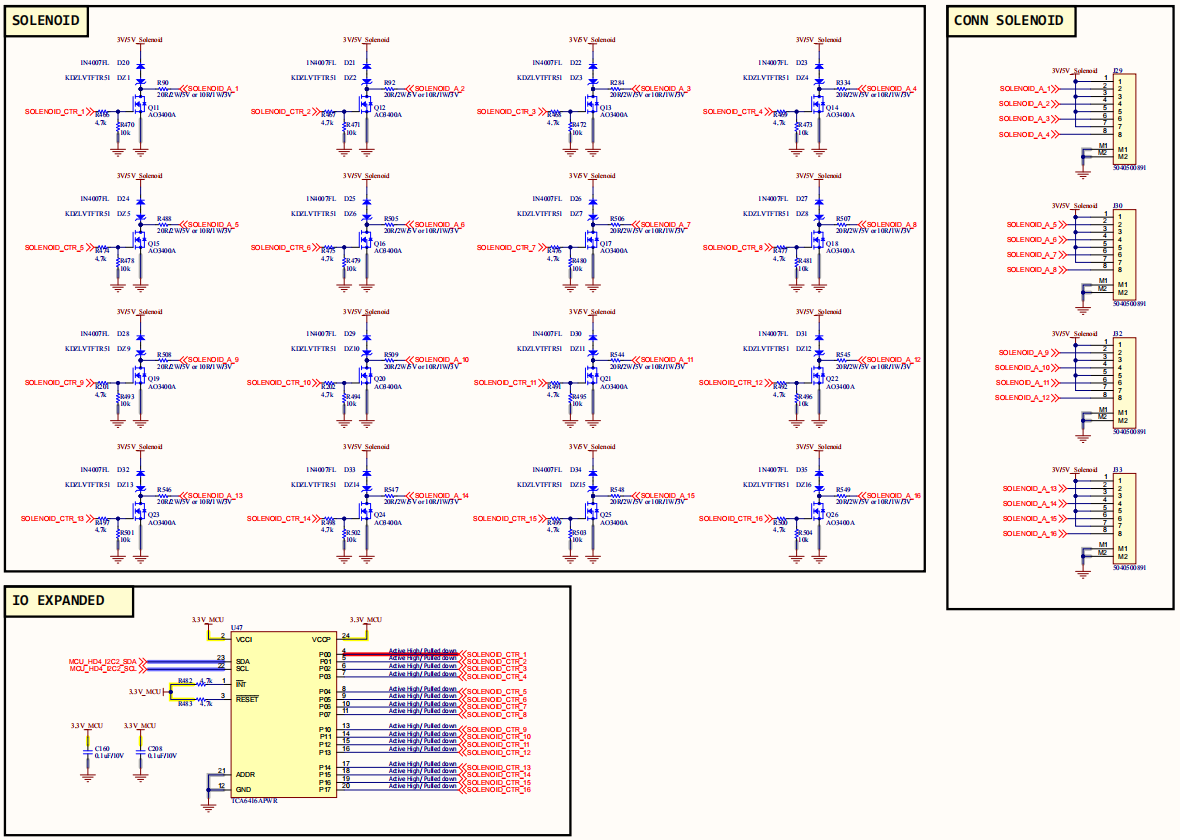
\includegraphics[width=1\textwidth]{picture/exp/solenoid-fet.png}
    \\caption{Sơ đồ nguyên lí khối điều khiển solenoid thứ 2}
    \label{fig:exp-sche-solenoid-fet}
\end{figure}

Sử dụng IC TCA6416A để mở rộng các pin I/O. TCA6416A là IC mở rộng 16-bit ngõ vào/ra (I/O) song song qua giao diện I2C hoặc SMBus. Thiết bị hoạt động dựa trên việc sử dụng các thanh ghi nội (cấu hình, ngõ vào, ngõ ra, đảo cực) để xác định hướng dữ liệu và trạng thái của 16 chân I/O. IC giao tiếp qua I2C, và các tín hiệu I/O. Tín hiệu ra gồm 16 cổng P-port (P00-P17) và một ngõ báo ngắt INT khi có sự thay đổi trạng thái ở ngõ vào. Ưu điểm của IC này là khả năng dịch mức điện áp hai chiều trong dải 1.65V đến 5.5V, dòng tiêu thụ ở chế độ chờ là 3 μA, các cổng I/O chịu được điện áp 5V và có khả năng tiêu tán dòng 25 mA.



\begin{figure}[H]
    \centering
    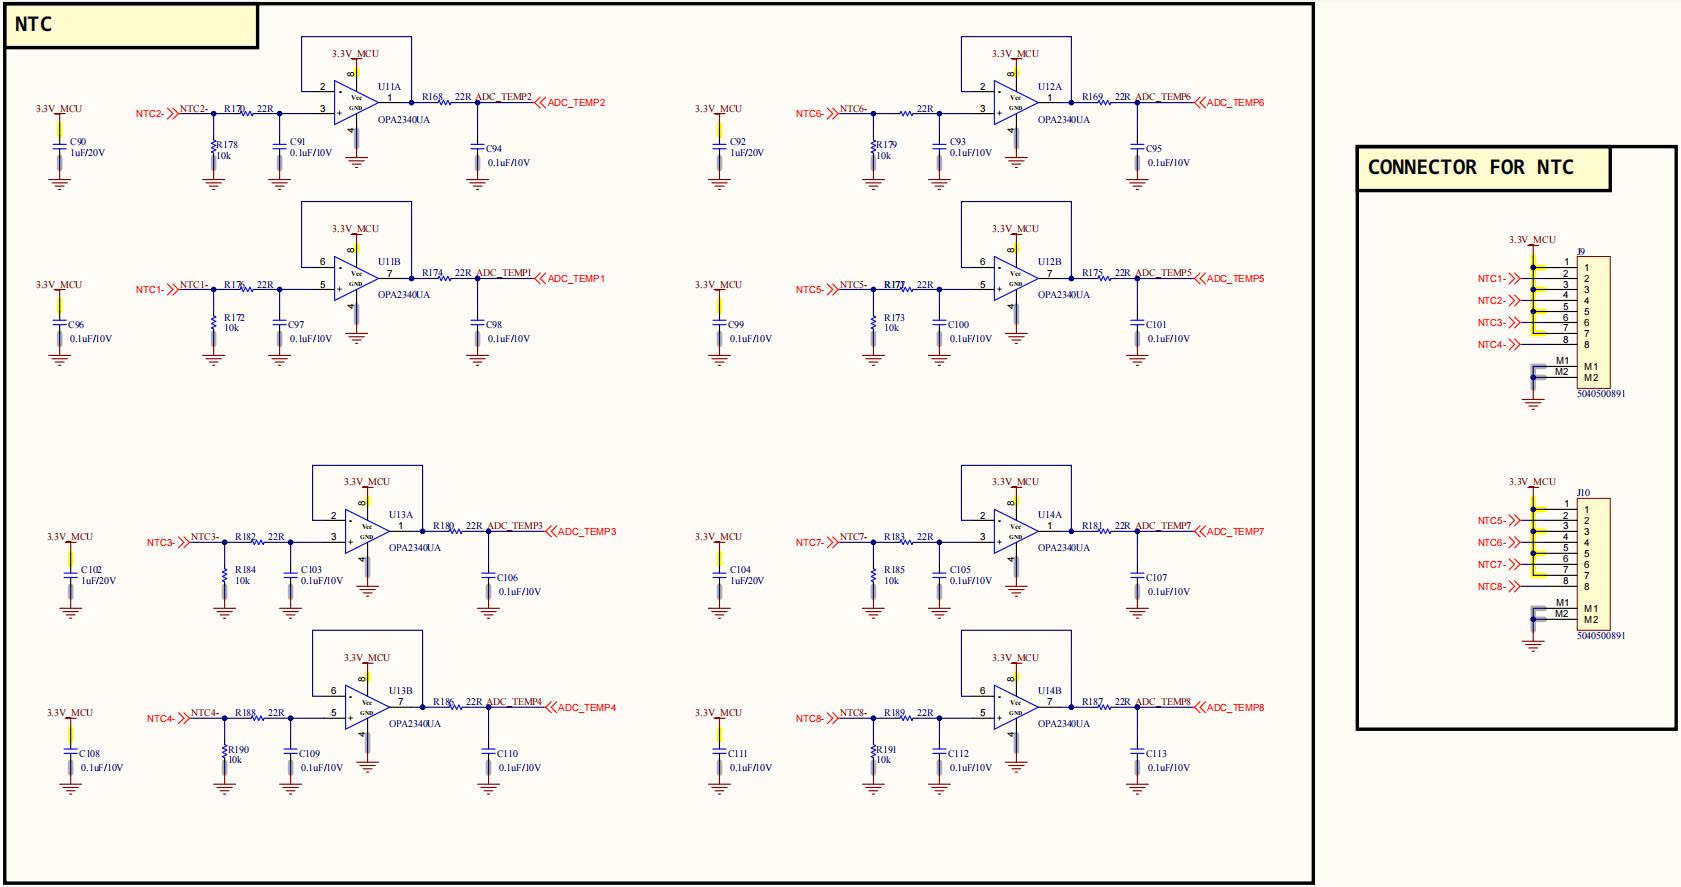
\includegraphics[width=1\textwidth]{picture/exp/khoi-ntc.jpg}
    \\caption{Sơ đồ nguyên lí khối NTC}
    \label{fig:exp-sche-khoi-ntc}
\end{figure}

Các cảm biến nhiệt được mắc lên buồng thí nghiệm ở các vị trí theo yêu cầu, tín hiệu được đọc về thông qua connector for NTC, các tín hiệu áp trên NTC sẽ đi qua một mạch đệm opamp và vào chân ADC của MCU. Các tín hiệu ADC sẽ được cân chỉnh và tính toán bằng phần mềm. 

Trong kênh đo nhiệt độ, mỗi NTC loại 10~k$\Omega$ tại 25$^\circ$C được ghép với một điện trở chuẩn 10~k$\Omega$ theo cấu hình cầu phân áp kéo xuống. Điện áp tại nút đo được xác định bởi:
\begin{equation}
V_{NTC-}=3V3\_MCU\times\frac{R_{pull-down}}{R_{NTC}+R_{pull-down}}=3.3\times\frac{10000}{R_{NTC}+10000}
\end{equation}

Với đặc tính NTC, khi nhiệt độ tăng thì $R_{NTC}$ giảm nên $V_{NTC-}$ tăng; ngược lại, khi nhiệt độ giảm thì $R_{NTC}$ tăng và $V_{NTC-}$ giảm. Nhờ đó, hệ thống thu được tín hiệu analog biến thiên liên tục để MCU đưa vào bộ ADC.

\begin{figure}[H]
    \centering
    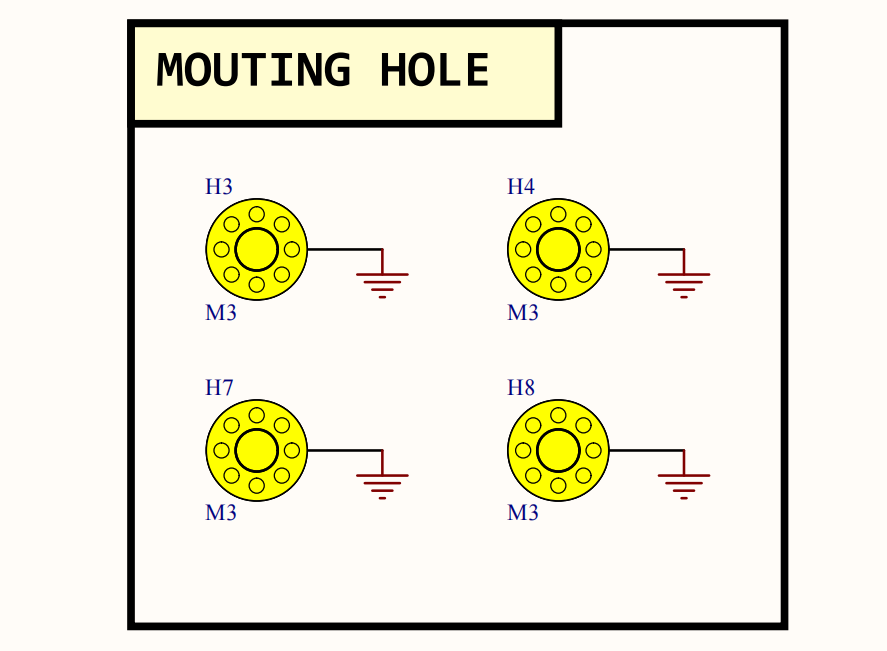
\includegraphics[width=0.5\textwidth]{picture/exp/hole.png}
    \\caption{Sơ đồ nguyên lí khối hole (cơ khí/tiếp địa)}
    \label{fig:exp-sche-hole}
\end{figure}

Các mounting hole phục vụ cố định cơ khí và/hoặc tiếp địa tham chiếu cho PCB, góp phần nâng độ bền và ổn định nhiễu EMC.


/% SUBSECTION FOR BOARD IF %/
\subsection{Board giao tiếp - IF}
\label{subsec:sche-board-giao-tiep-if}

\begin{figure}[H]
    \centering
    \begin{minipage}{0.49\textwidth}
        \centering
        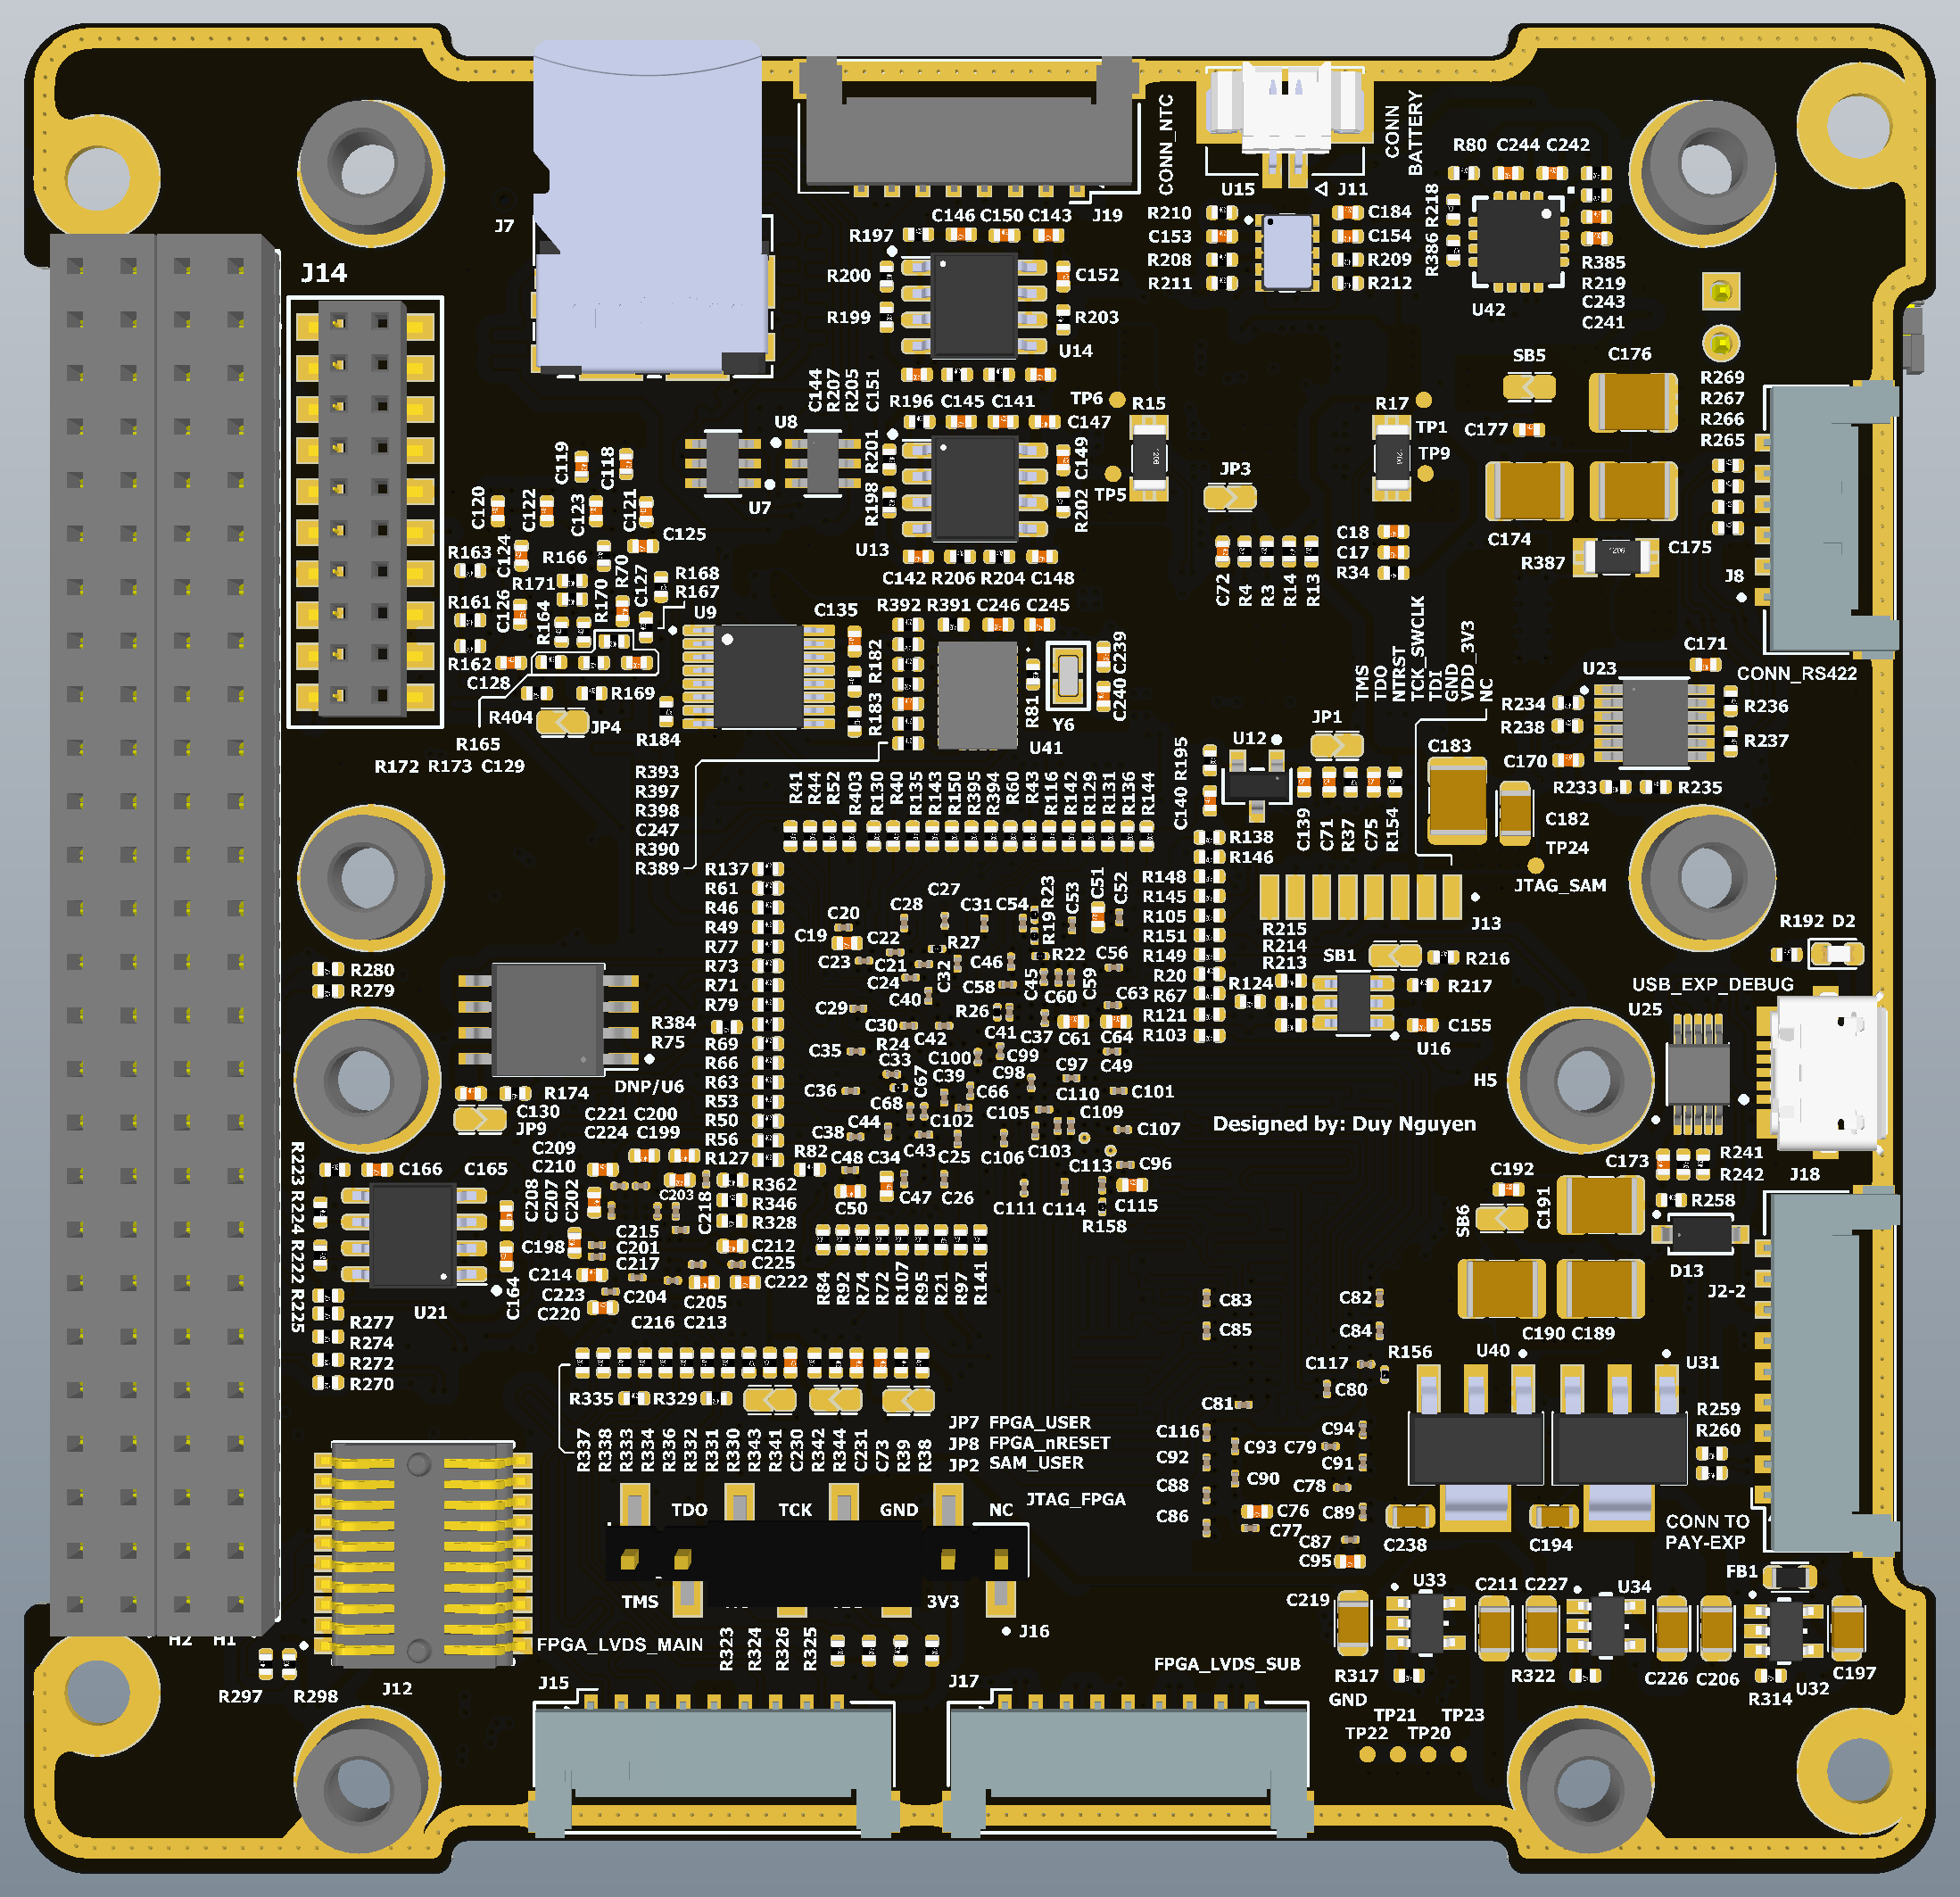
\includegraphics[width=\textwidth]{picture/if/BEE-1012 PAY-IF V1.1.0.png}
        
        Mặt trên
    \end{minipage}
    \hfill
    \begin{minipage}{0.49\textwidth}
        \centering
        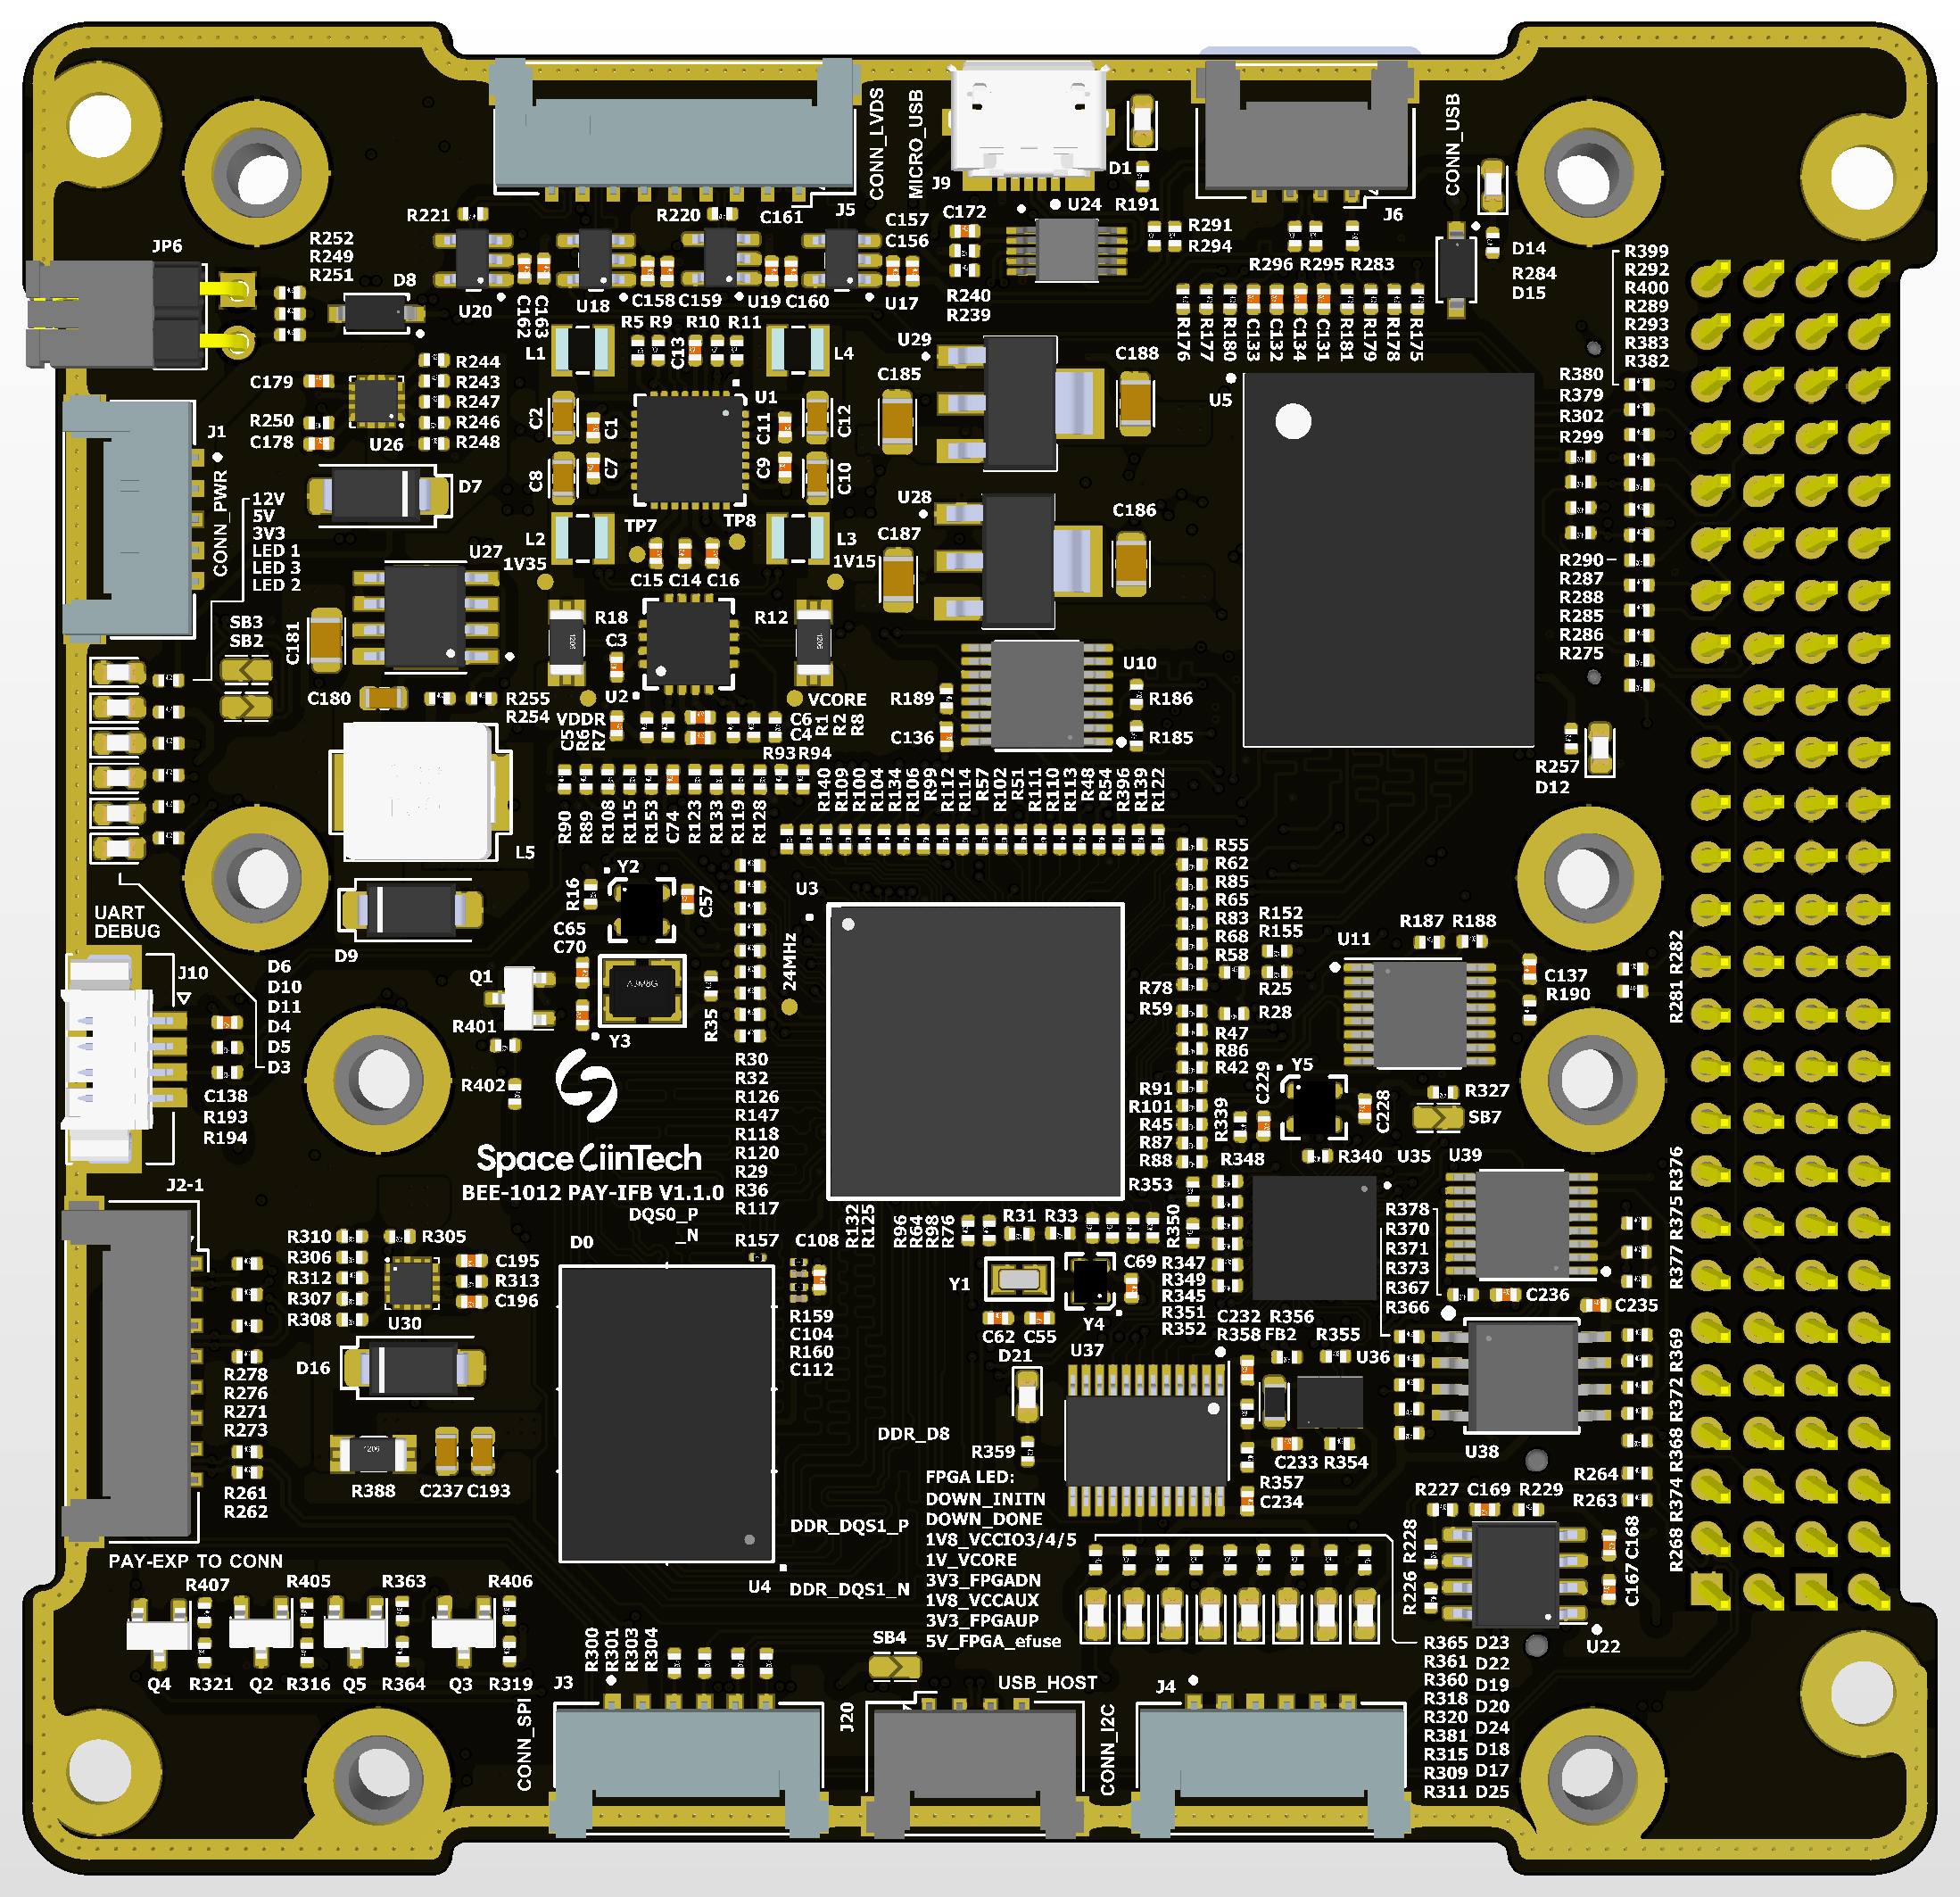
\includegraphics[width=\textwidth]{picture/if/BEE-1012 PAY-IF V1.1.0-bot.png}
        
        Mặt dưới
    \end{minipage}
    \caption{PCB board IF}
    \label{fig:if-pcb-board}
\end{figure}

\begin{figure}[H]
    \centering
    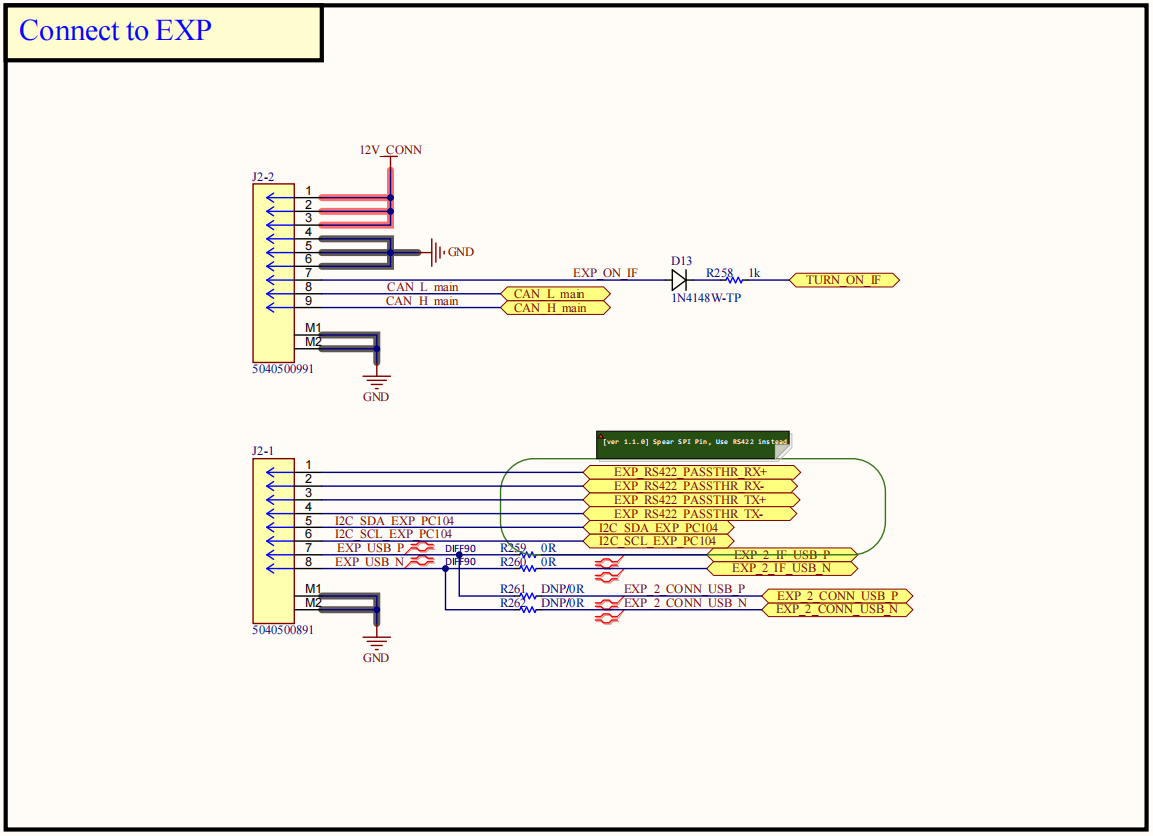
\includegraphics[width=1\textwidth]{picture/if/connector-exp.png}
    \\caption{Sơ đồ nguyên lí khối connector-exp}
    \label{fig:if-connector-exp}
\end{figure}

Các tín hiệu giao tiếp với board EXP bao gồm CAN, RS422, I2C, USB, và một tín hiệu enable efuse 12V trên board IF. Ở trạng thái bình thường, mặc định board IF sẽ tắt, khi nhận được tín hiệu enable của board EXP điều khiển nó mới bật efuse 12V trên IF, từ thời điểm đó board IF mới bắt đầu có nguồn.

\begin{figure}[H]
    \centering
    
\includegraphics[width=0.9\textwidth]{\detokenize{picture/if/efuse-12v-mpu .png}}
    \caption{eFuse 12V cho MPU}
    \label{fig:if-efuse-12v-mpu}
\end{figure}

Khối efuse trên board IF được thiết kế như một công tắc nguồn cho cả board và phải được enable bởi tín hiệu TURN\_ON\_IF ở chân EN của IC. Thông thường board IF sẽ ở trạng thái tắt hoàn toàn do dòng điện chỉ đến được đầu vào của efuse. Khi có tính hiệu enable kéo lên mức cao được lái bởi tín hiệu trong bus connector với board EXP, từ VBUS khi người dùng cắm tín hiệu USB debug và một jumper kéo lên nguồn thủ công. Các thông số thiết kế ngưỡng dòng áp đều được giữ nguyên giống như cách thiết kế trên board EXP.

\begin{figure}[H]
    \centering
    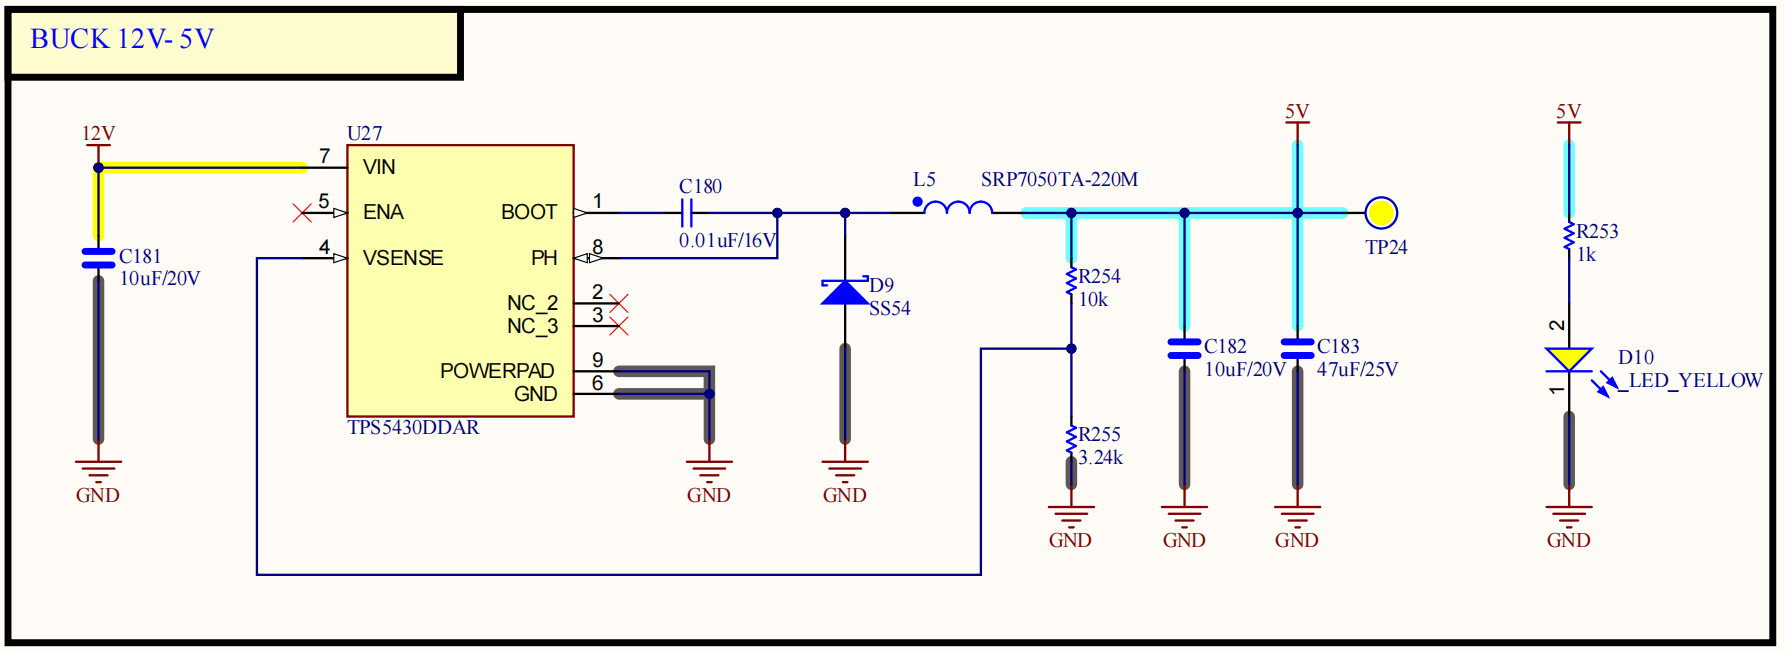
\includegraphics[width=0.9\textwidth]{picture/if/buck-12v-5v.png}
    \caption{Mạch buck từ 12V sang 5V}
    \label{fig:if-buck-12v-5v}
\end{figure}

Tương tự như cách thiết kế mạch nguồn buck từ 12V sang 5V trên board EXP. 

\begin{figure}[H]
    \centering
    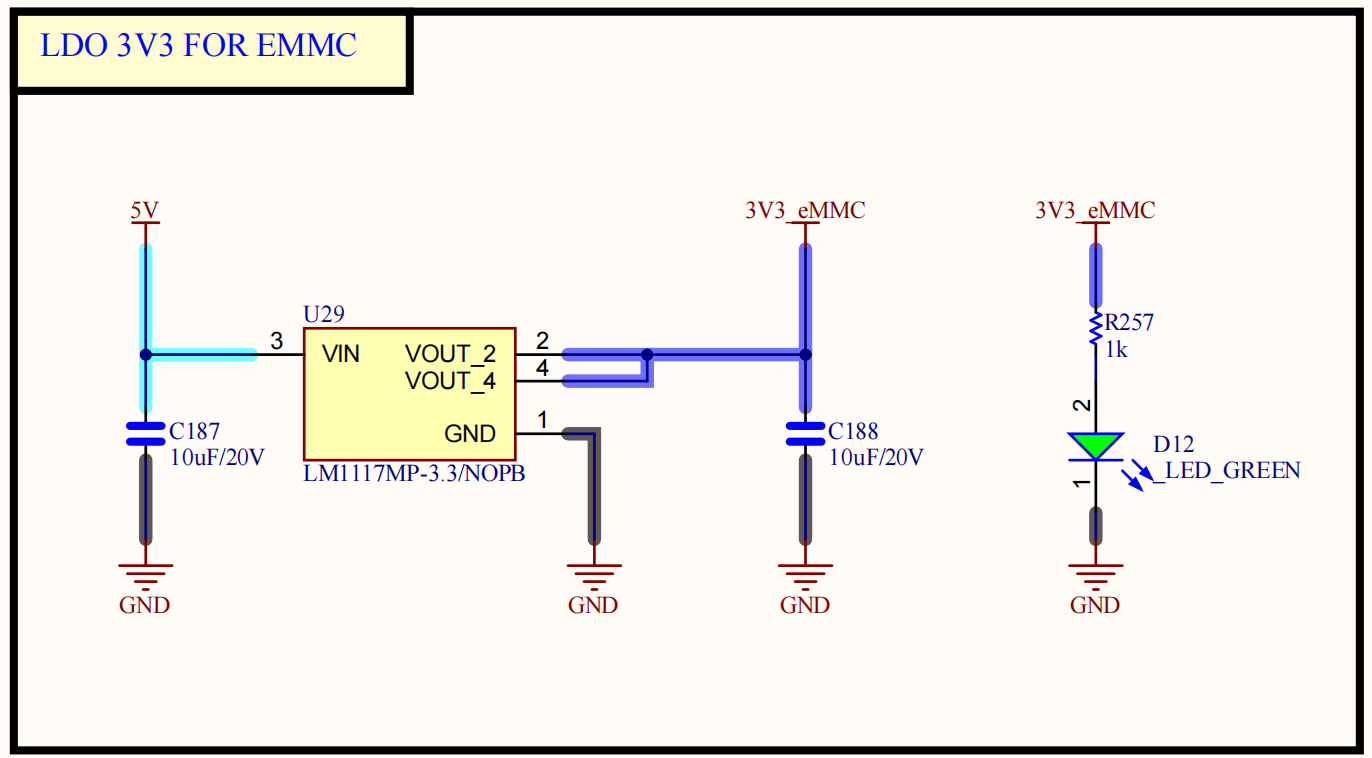
\includegraphics[width=0.7\textwidth]{picture/if/ldo-3v3-emmc.png}

    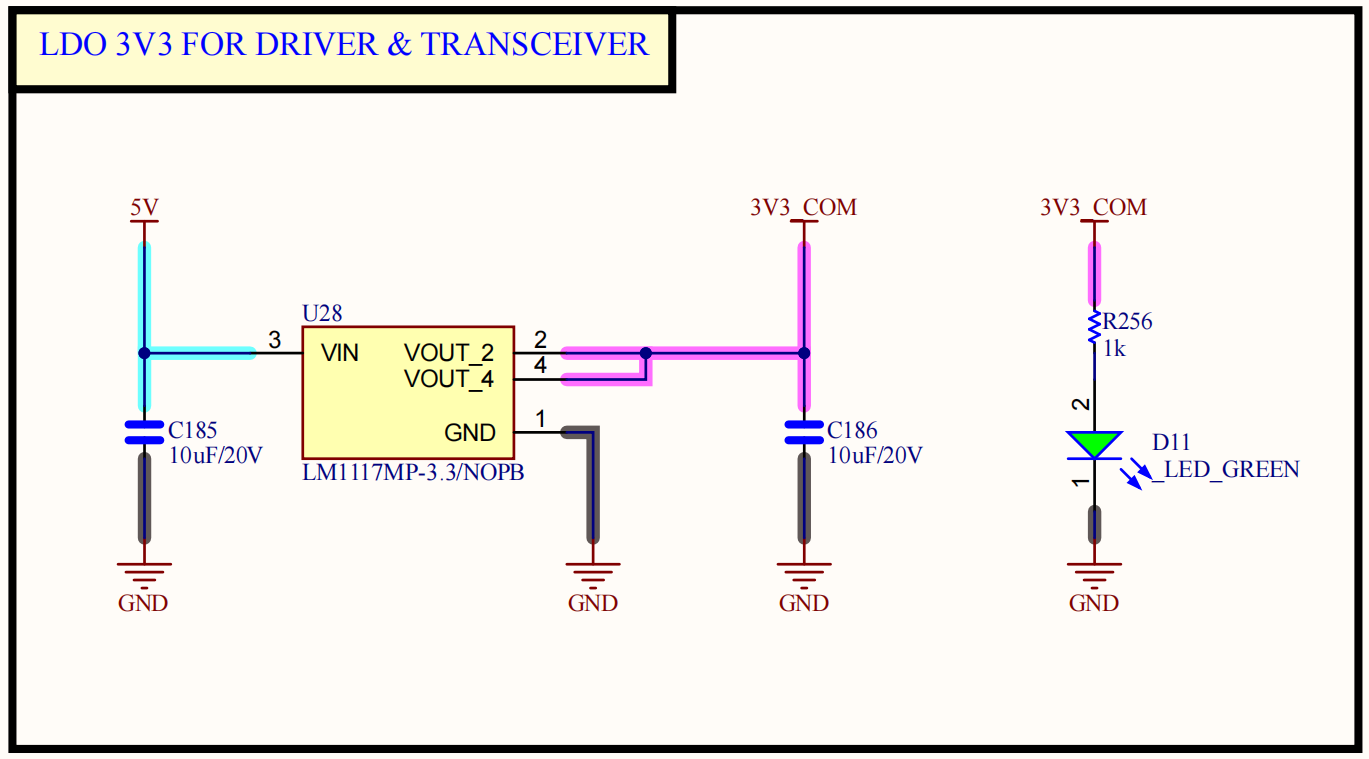
\includegraphics[width=0.7\textwidth]{picture/if/ldo-3v3-driver.png}
    \caption{LDO 3V3 cho các IC trên board}
    \label{fig:if-ldo-3v3-ics}
\end{figure}

eMMC có LDO riêng do thông thường eMMC sẽ kéo dòng khá lớn trong quá trình đọc ghi, có thể làm dòng và áp không ổn định ảnh hưởng lên các ngoại vi khác nên dùng riêng LDO từ 5V xuống 3V3\_eMMC cho eMMC ở khối LDO 3V3 FOR EMMC. Còn các IC driver, transceiver hay các giao tiếp khác cần nguồn cấp 3V3 sẽ dùng từ 3V3\_COM ở LDO 3V3 FOR DRIVER \& TRANSCEIVER.

\begin{figure}[H]
    \centering
    \begin{minipage}[t]{0.495\textwidth}
        \centering
        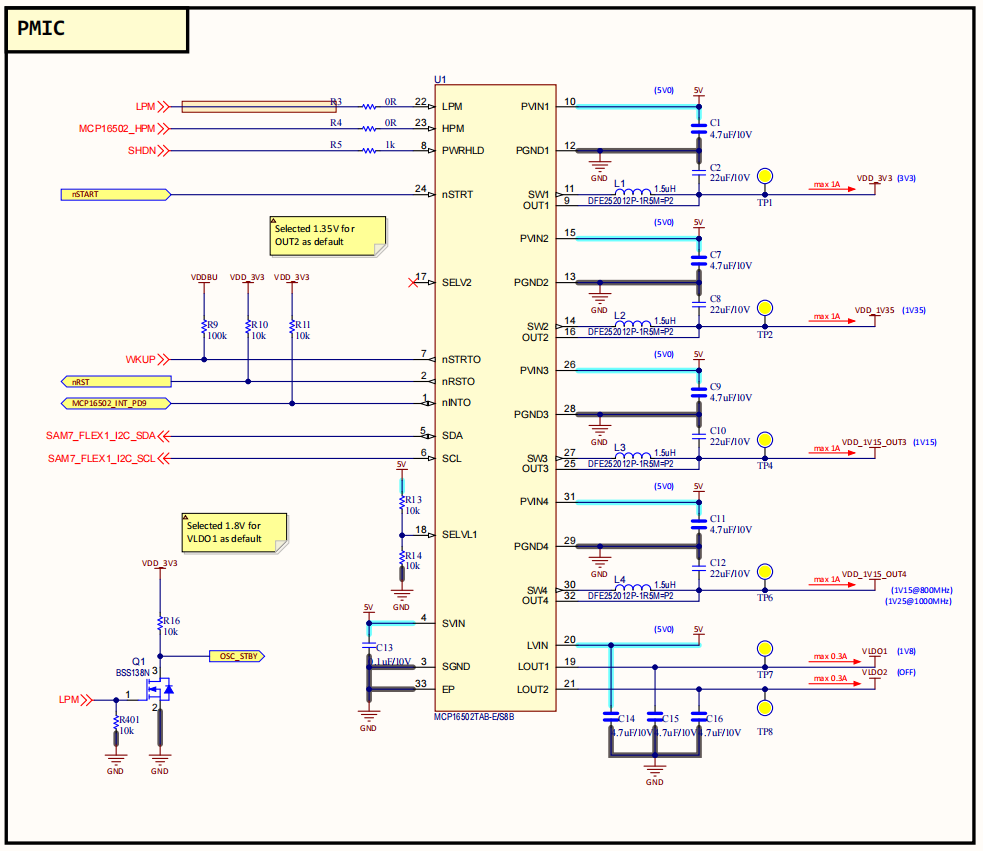
\includegraphics[width=\textwidth,height=0.30\textheight,keepaspectratio]{picture/if/pmic.png}
        \captionof{figure}{Khối quản lý nguồn PMIC}
        \label{fig:if-pmic}
    \end{minipage}\hspace{0.01\textwidth}%
    \begin{minipage}[t]{0.495\textwidth}
        \centering
        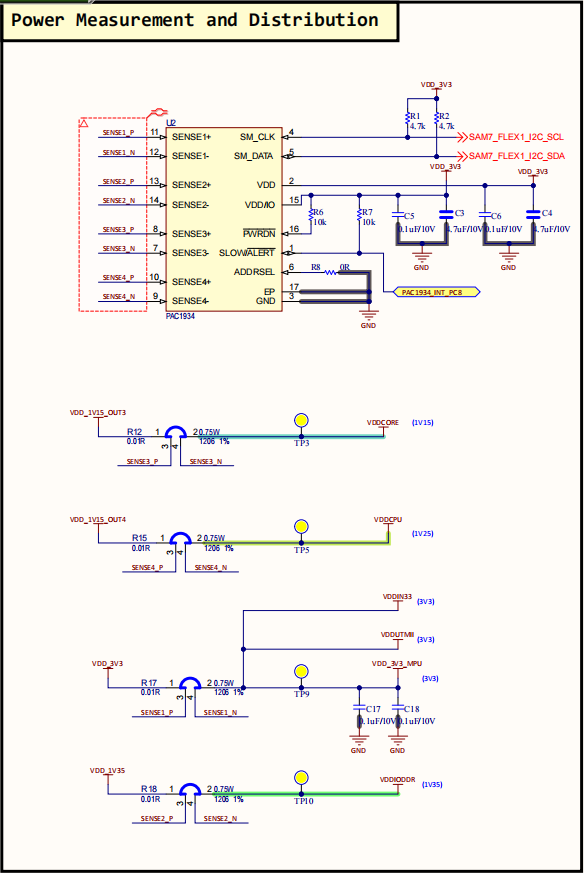
\includegraphics[width=\textwidth,height=0.30\textheight,keepaspectratio]{picture/if/power-measurement-mpu.png}
        \captionof{figure}{Khối đo nguồn}
        \label{fig:if-power-measurement-mpu}
    \end{minipage}
\end{figure}

Tương tự như trên bo EXP, bo IF dùng chung thiết kế MPU nên khối quản lý nguồn và khối đo nguồn cũng được dùng tương tự. Những thiết kế như thế được đề xuất thiết kế trong datasheet của con chip SAMA7G54 để đảm bảo hệ thống hoạt động ổn định, tận dụng thiết kế phần cứng và phần mềm sẵn có.

\begin{figure}[H]
    \centering
    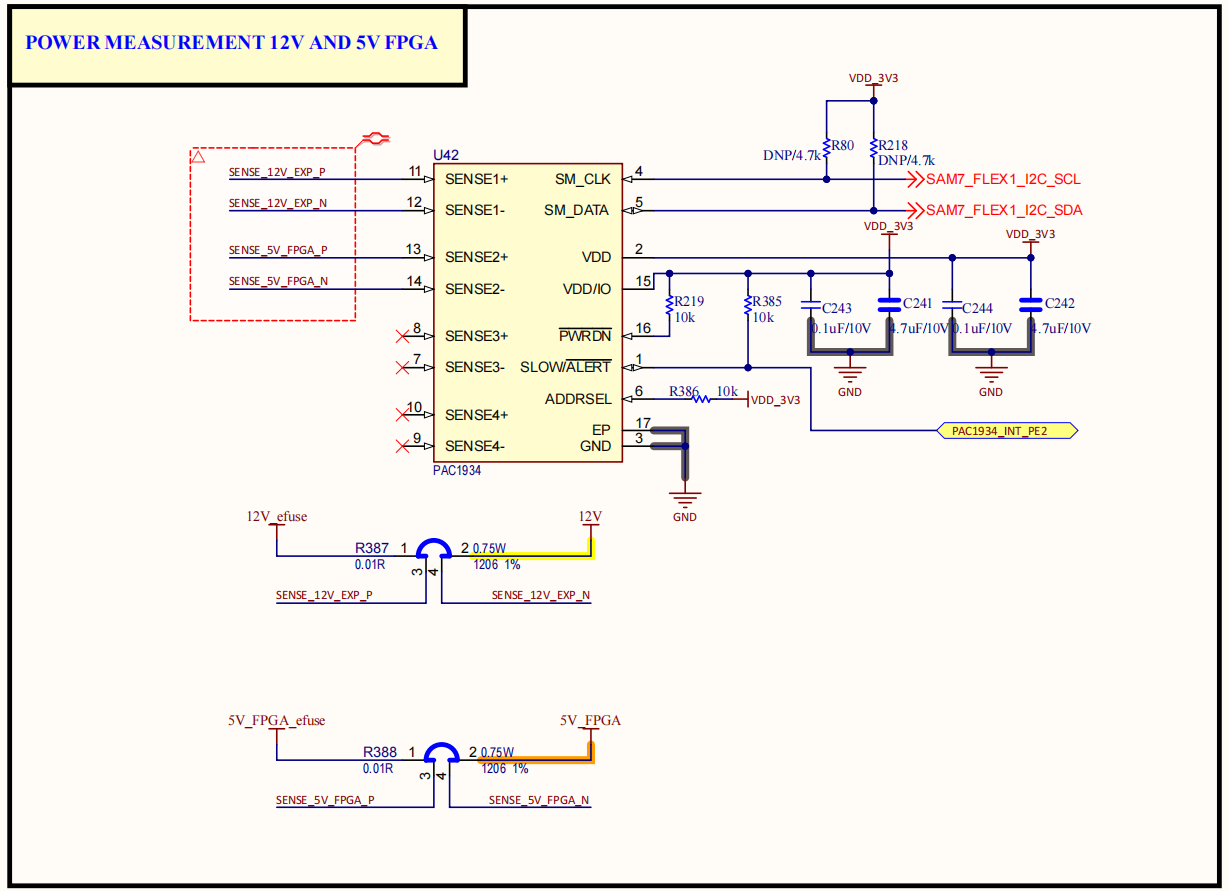
\includegraphics[width=1\textwidth]{picture/if/powrer-measurement-12V-5VFPGA.png}
    \\caption{Sơ đồ nguyên lí khối đo nguồn 12V và 5V\_FPGA}
    \label{fig:if-powrer-measurement-12V-5VFPGA}
\end{figure}

Bên cạnh dùng PAC1934 để đo dòng tải trên các nguồn MPU tiêu thụ, board IF dùng thêm một PAC1934 để có thể theo dõi được dòng tải trên cả board thông qua RSHUNT trên đường nguồn 12V cho cả board (12V\_EXP) và kiểm soát dòng tiêu thụ từ FPGA và các thành phần liên quan qua trở RSHUNT trên đường 5V\_FPGA.

\begin{figure}[H]
    \centering
    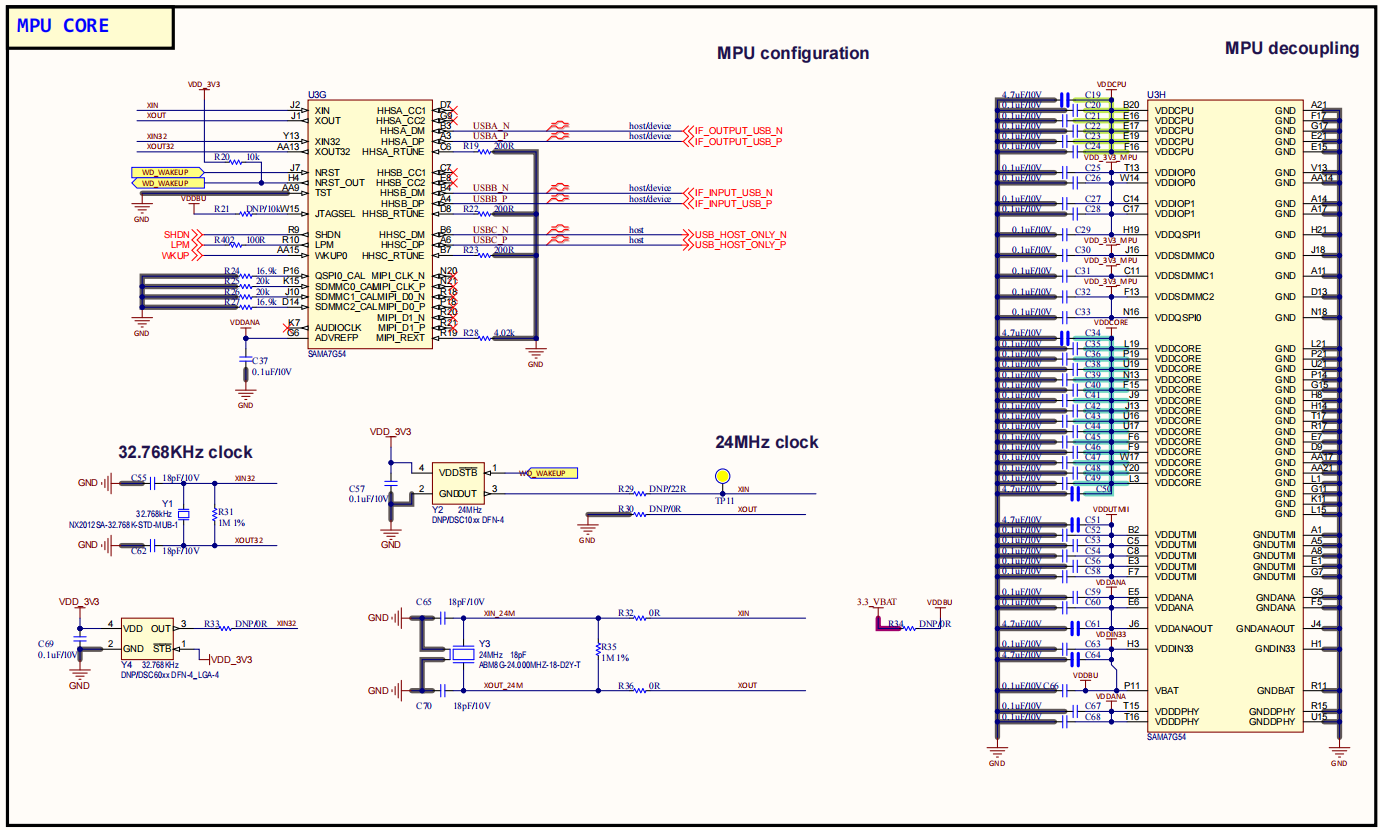
\includegraphics[width=1\textwidth]{picture/if/mpu-core.png}
    \\caption{Sơ đồ nguyên lí khối MPU core}
    \label{fig:if-mpu-core}
\end{figure}

\begin{figure}[H]
    \centering
    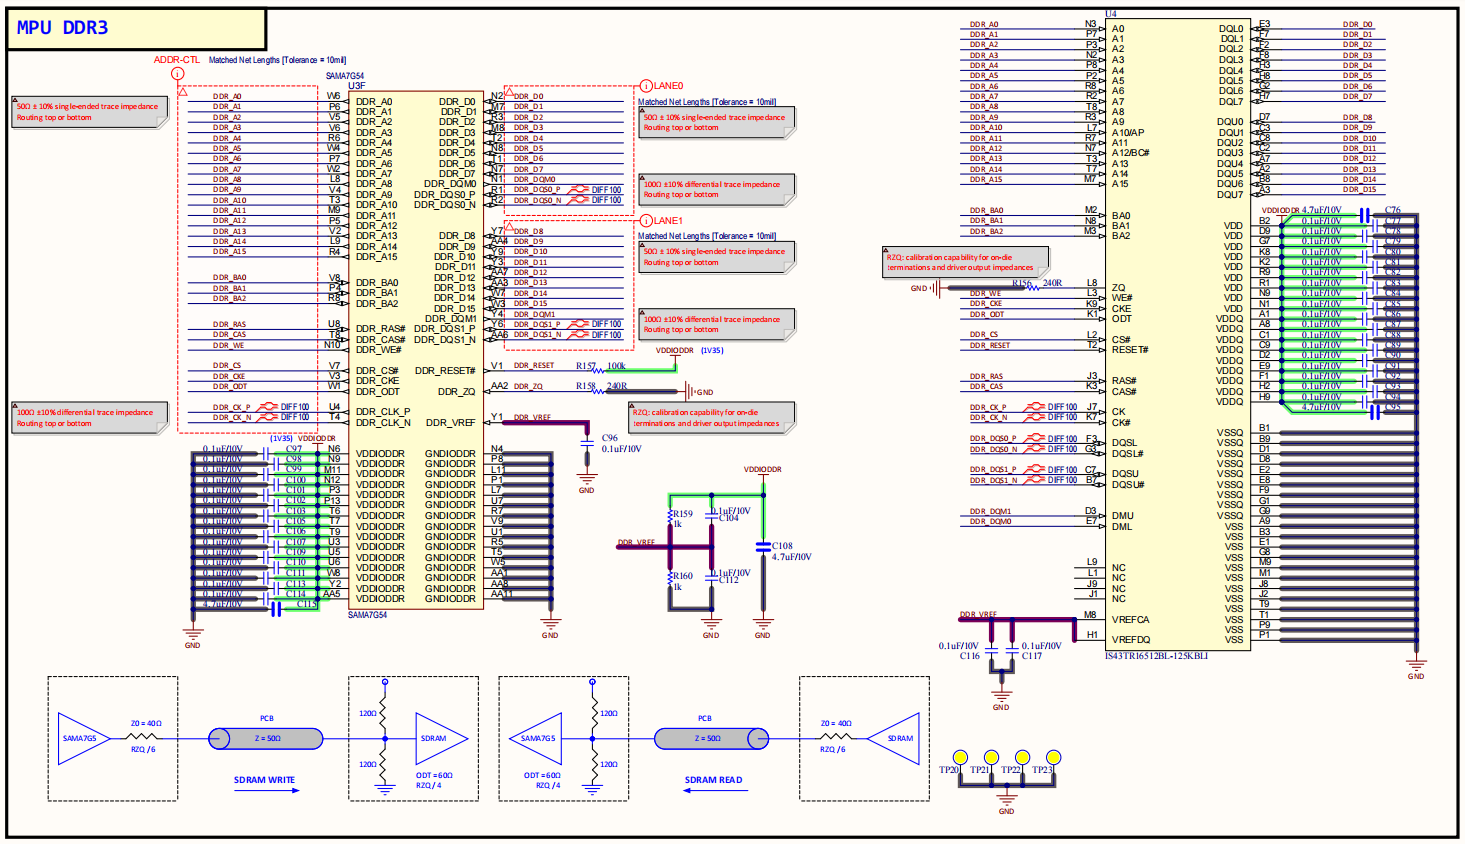
\includegraphics[width=1\textwidth]{picture/if/mpu-ddr.png}
    \caption{MPU giao tiếp với DRAM (DDR3)}
    \label{fig:if-mpu-ddr}
\end{figure}

IC DRAM dùng cùng part number là IS43TR16512BL-125KBLI tương tự như trên board EXP để tối ưu sử dụng firmware. 


\begin{figure}[H]
    \centering
    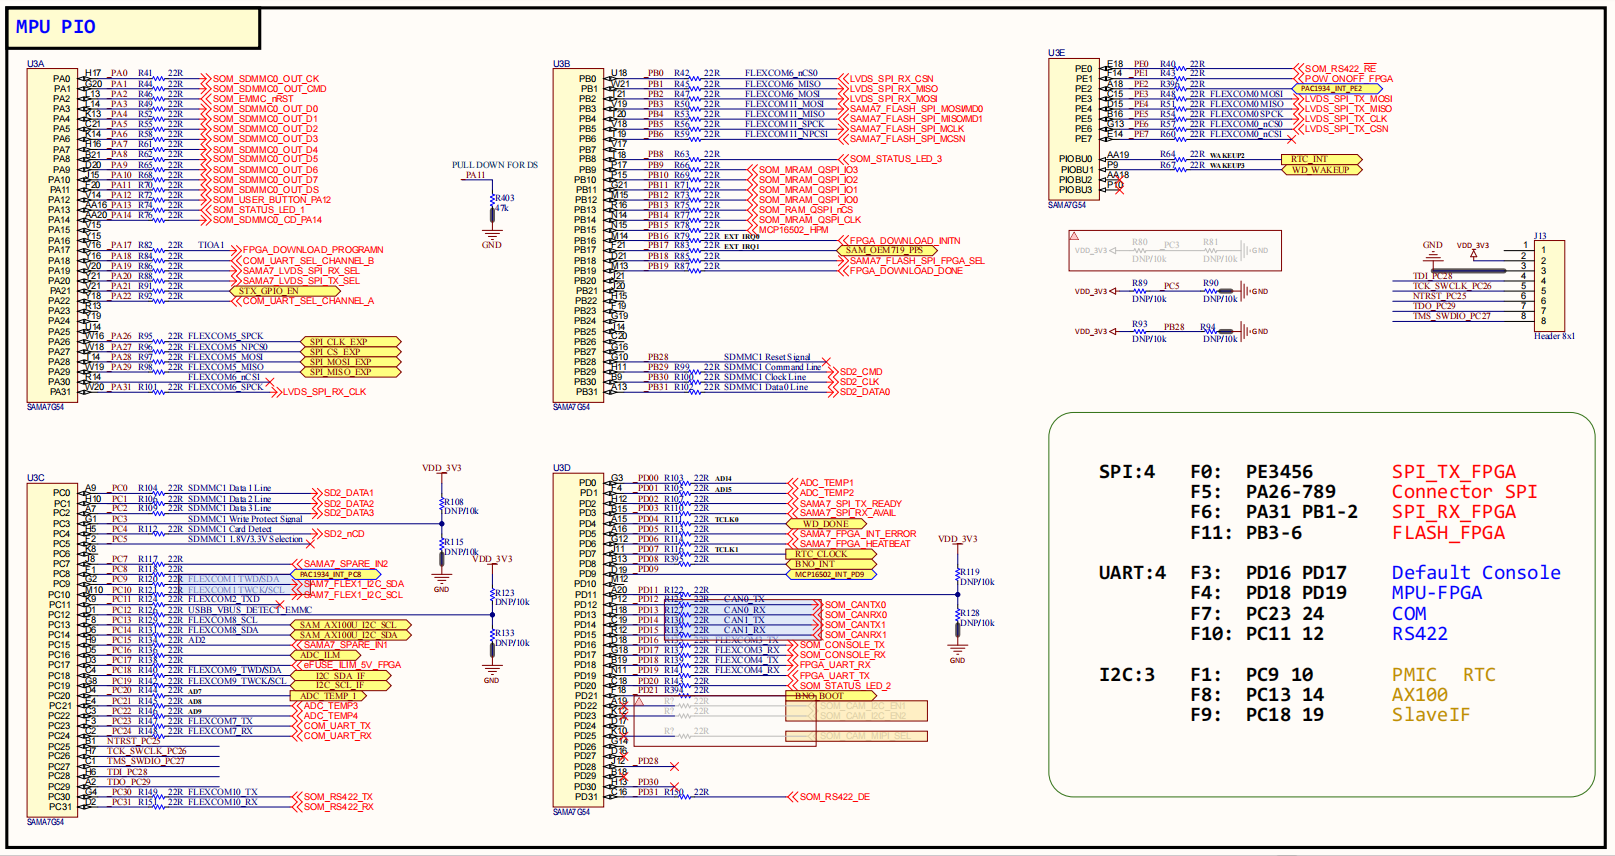
\includegraphics[width=1\textwidth]{picture/if/mpu-pio.png}
    \caption{Tín hiệu PIO trên MPU}
    \label{fig:if-fpga-pio}
\end{figure}

Các tín hiệu trên MPU bao gồm:

\begin{itemize}
    \item SDMMC: SDMMC0 cho eMMC, SDMMC cho SDCard.
    \item SPI: SPI switch TX/RX LVDS, SPI switch với FPGA để giao tiếp với SPI FLASH, connector SPI.
    \item I2C: các IC onboard như PMIC, RTC, connector I2C, connector PC104.
    \item UART: UART console, RS422, giao tiếp trực tiếp với FPGA.
    \item ADC: các tín hiệu ADC từ efuse, NTC, cảm biến nhiệt độ onboard.
    \item I/O: các tín hiệu ngắt, tín hiệu enable, tín hiệu điều khiển led status.
\end{itemize}

\begin{figure}[H]
    \centering
    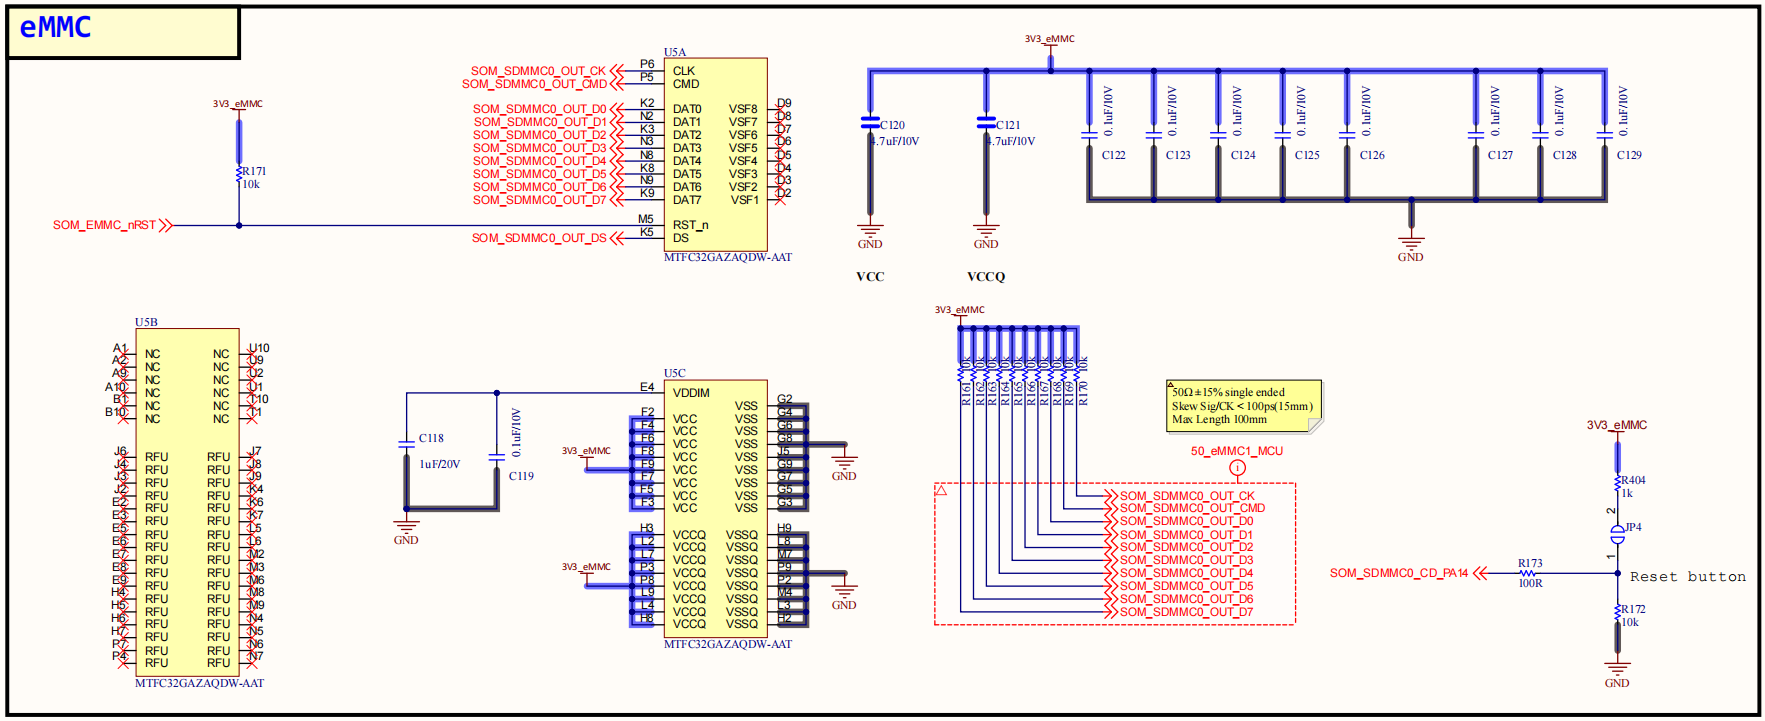
\includegraphics[width=0.9\textwidth]{picture/if/emmc.png}
    \caption{eMMC}
    \label{if-emmc}
\end{figure}

eMMC thường đóng vai trò bộ nhớ không mất dữ liệu chính của hệ MPU, dùng để lưu bootloader, kernel/device tree, root filesystem và dữ liệu ứng dụng. Theo mô hình SD/MMC phổ biến, eMMC có các vùng boot partition riêng, vùng user area và có thể có thêm RPMB cho dữ liệu bảo mật, nên phù hợp làm bộ nhớ hệ thống ổn định trong vận hành lâu dài. Thiết kế eMMC trên IF cũng tương tự như eMMC cho MPU trên board EXP.

\begin{figure}[H]
    \centering
    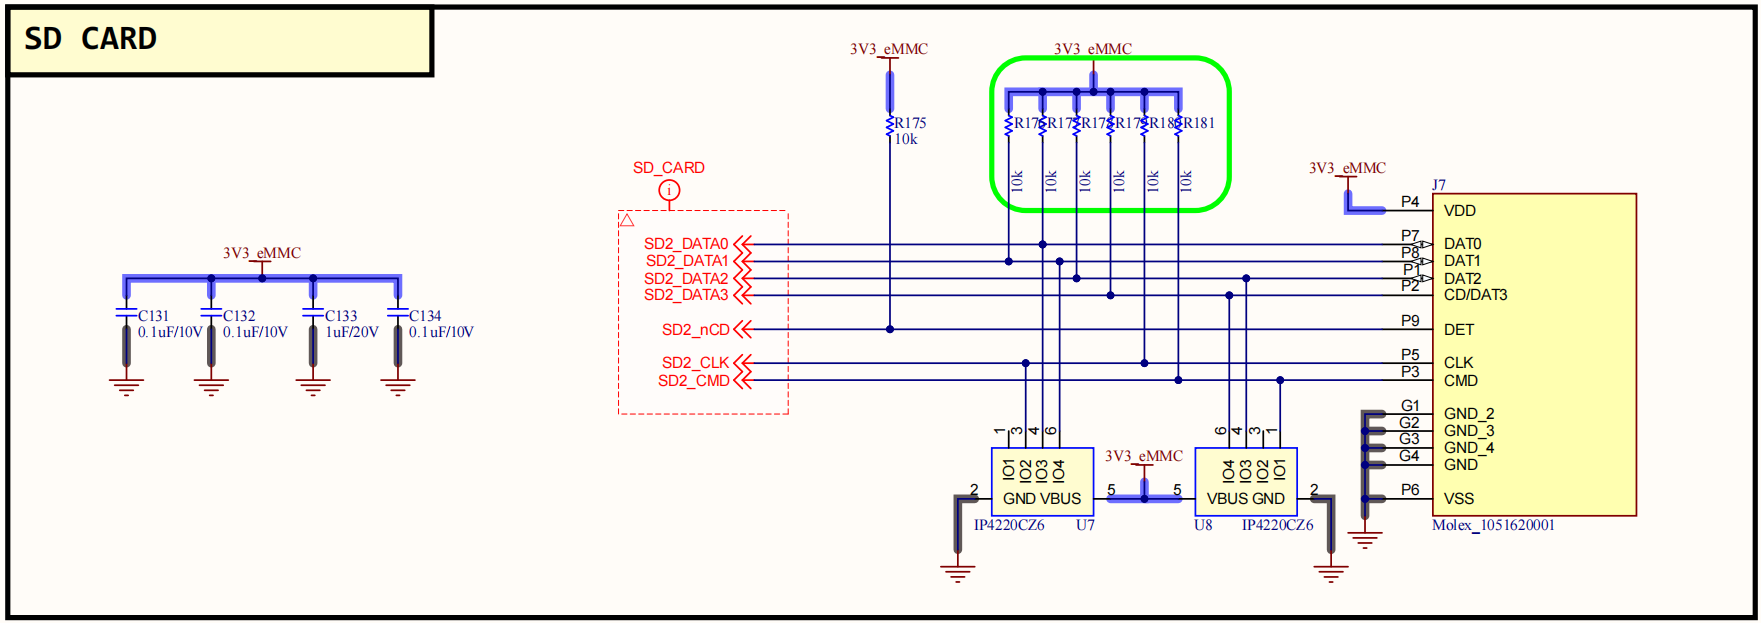
\includegraphics[width=0.9\textwidth]{picture/if/sdcard.png}
    \caption{SDCard cho MPU}
    \label{if-sdcard}
\end{figure}

SD Card được bổ sung cho MPU nhằm tăng tính linh hoạt trong phát triển và bảo trì hệ thống: có thể boot tạm thời khi eMMC chưa nạp image, phục hồi khi hệ thống trên eMMC lỗi, và triển khai/cập nhật phần mềm nhanh bằng cách thay thẻ nhớ mà không cần can thiệp sâu vào bộ nhớ hàn trên bo. Vì vậy trong thực tế, eMMC thường là bộ nhớ vận hành chính, còn SD Card phù hợp cho giai đoạn bring-up, debug và cứu hộ.

\begin{figure}[H]
    \centering
    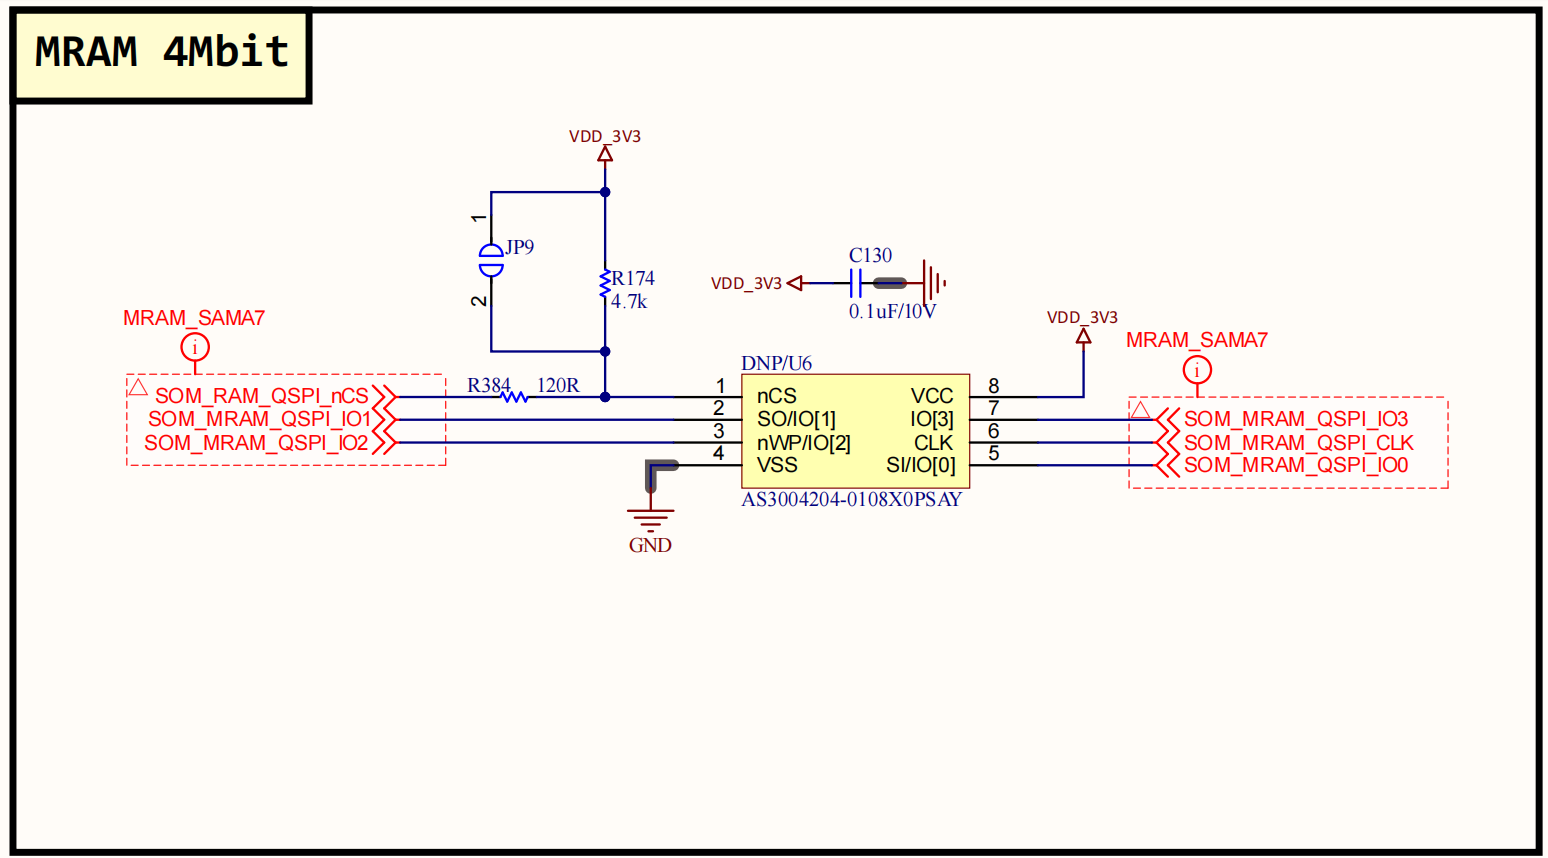
\includegraphics[width=0.8\textwidth]{picture/if/mram.png}
    \\caption{Sơ đồ nguyên lí khối MRAM}
    \label{fig:if-mram}
\end{figure}

MRAM vẫn sử dụng part number AS3004204-0108X0PSAY như trên thiết kế board EXP, nhưng trong thiết kế IF, IC này chưa được sử dụng nên đang thiết kế DNP.

\begin{figure}[H]
    \centering
    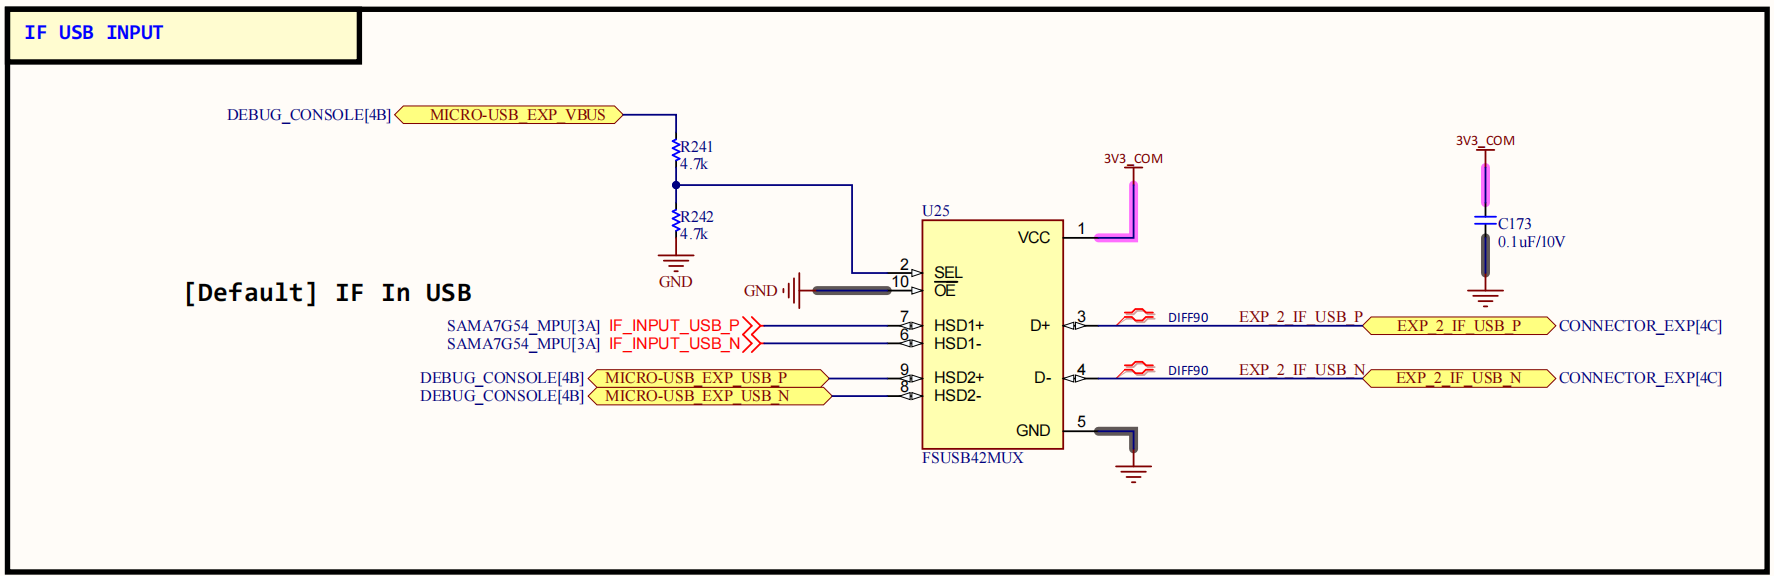
\includegraphics[width=1\textwidth]{picture/if/if-usb-sw-in.png}
    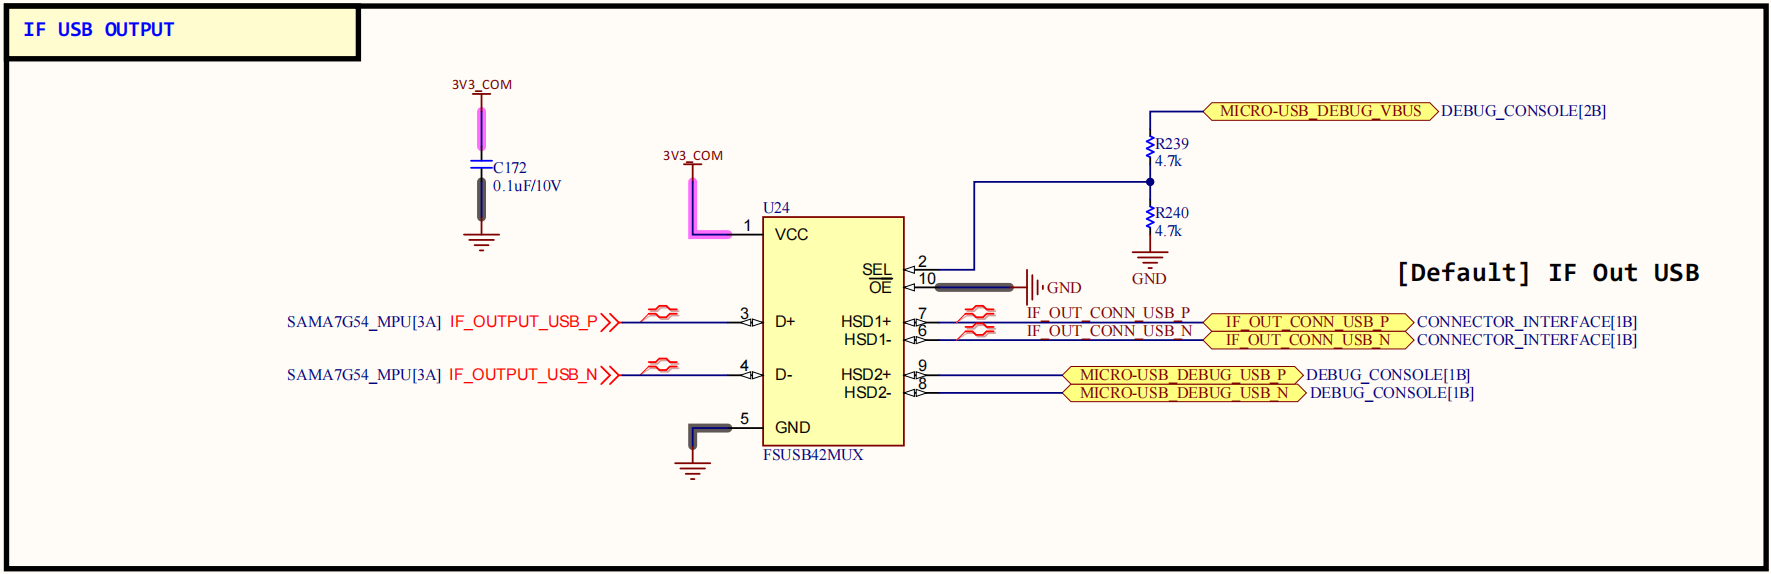
\includegraphics[width=1\textwidth]{picture/if/if-usb-sw-out.png}
    \\caption{Sơ đồ nguyên lí khối USB switch}
    \label{fig:if-usb-sw}
\end{figure}

FSUSB42 là bộ chuyển mạch DPDT hai chiều, công suất thấp, được thiết kế để chuyển đổi giữa các nguồn dữ liệu USB 2.0 hoặc UART. Thiết bị hoạt động dựa trên việc điều hướng tín hiệu từ cổng chung (D+/D-) đến một trong hai cổng đầu vào (HSD1 hoặc HSD2) thông qua chân điều khiển SEL, trong khi chân OE cho phép ngắt kết nối hoàn toàn để tiết kiệm điện. Ưu điểm của FSUSB42 bao gồm băng thông rộng (>720 MHz) và điện dung cực thấp (3.7 pF) giúp bảo toàn chất lượng tín hiệu, tiêu thụ điện năng tối thiểu (1 µA), cùng khả năng chịu quá áp (OVT) lên đến 5.25V ngay cả khi không có nguồn VCC, giúp bảo vệ an toàn cho các thiết bị di động hiện đại.

\begin{figure}[H]
    \centering
    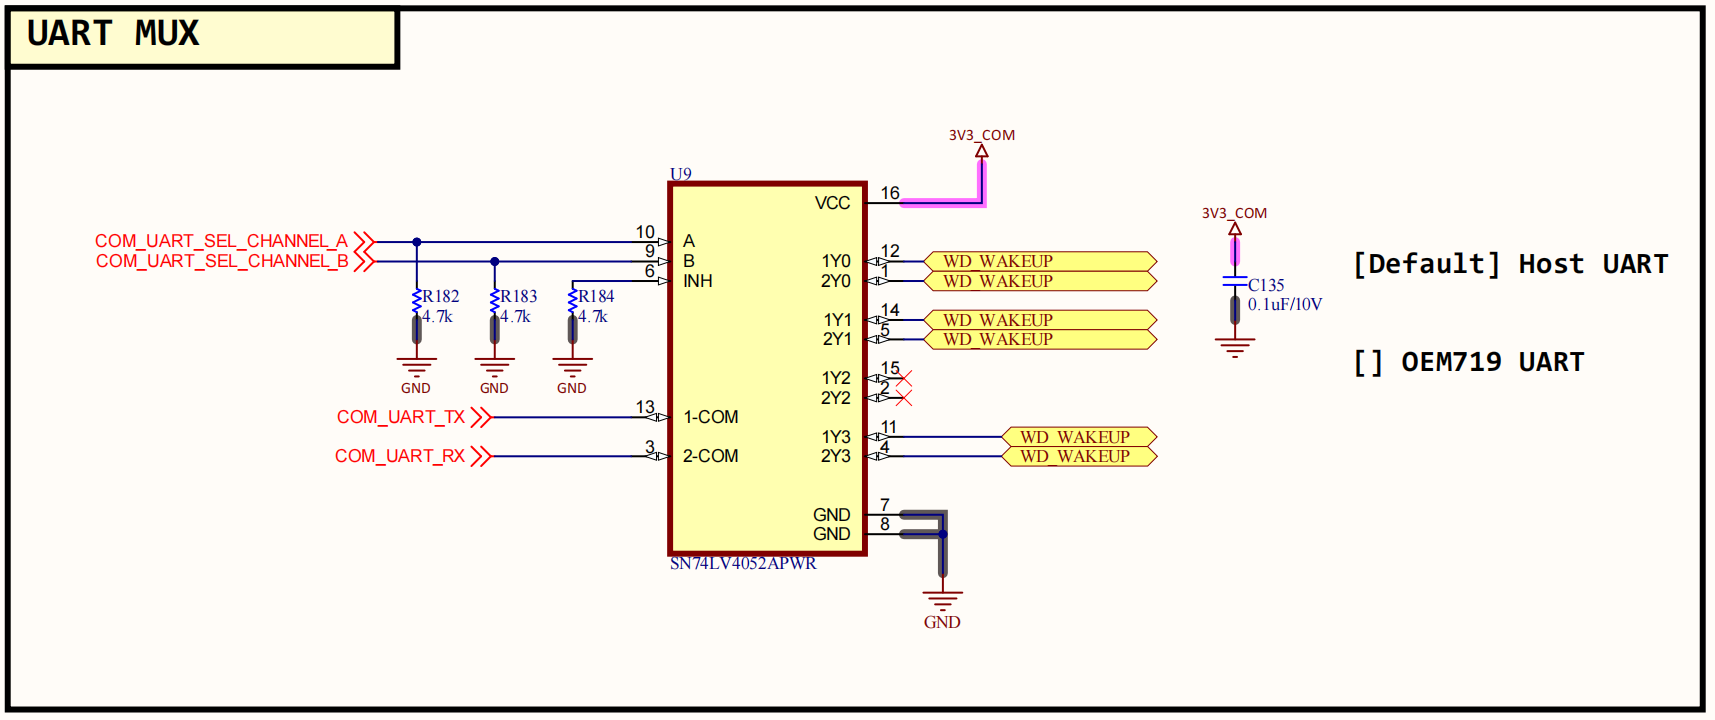
\includegraphics[width=0.9\textwidth]{picture/if/uart-mux.png}
    \\caption{Sơ đồ nguyên lí khối UART MUX}
    \label{fig:if-uart-mux}
\end{figure}

Thiết bị SN74LV4052A là một bộ ghép kênh và tách kênh tương tự CMOS 4 kênh kép, được thiết kế để xử lý linh hoạt cả tín hiệu tương tự và kỹ thuật số theo hai chiều với biên độ tối đa 5,5V. Nguyên lý hoạt động của thiết bị dựa trên việc điều khiển các chân logic: khi chân Inhibit (INH) ở mức thấp, các tổ hợp đầu vào của chân A và B sẽ chọn kết nối một trong bốn kênh độc lập (nY0-nY3) với kênh chung (n-COM); khi chân INH ở mức cao, tất cả các kênh sẽ chuyển sang trạng thái trở kháng cao (ngắt kết nối). Những ưu điểm nổi bật của linh kiện này bao gồm dải điện áp hoạt động rộng (1,65V đến 5,5V), tốc độ chuyển mạch nhanh, mức nhiễu chéo giữa các công tắc rất thấp, tiêu thụ dòng điện đầu vào cực nhỏ và tích hợp khả năng bảo vệ chống tĩnh điện (ESD) mạnh mẽ lên đến ±4000V

\begin{figure}[H]
    \centering
    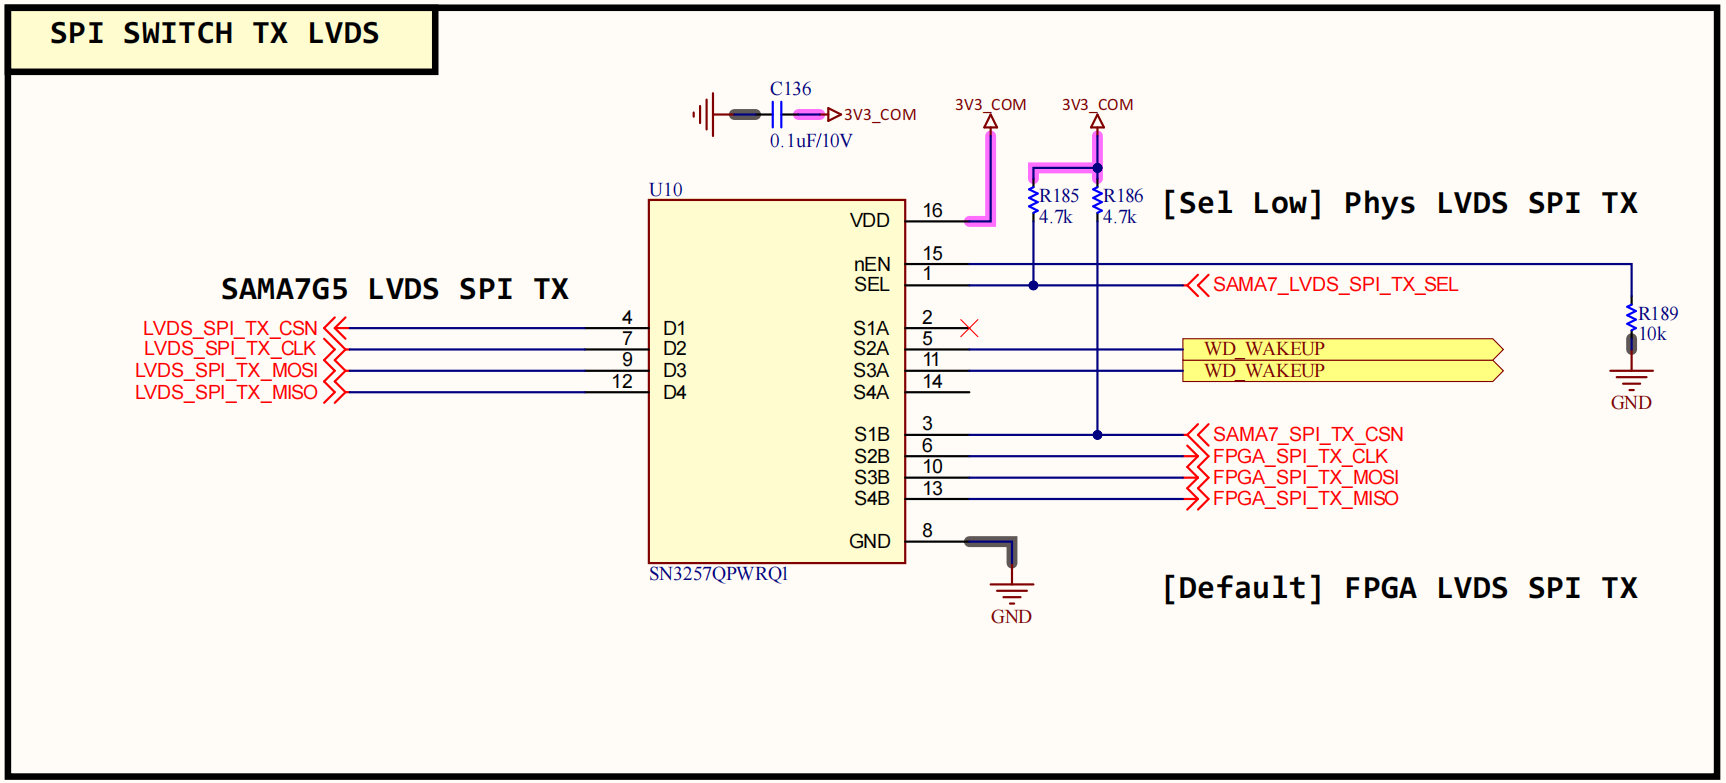
\includegraphics[width=0.9\textwidth]{picture/if/spi-sw-lvds-tx.png}
    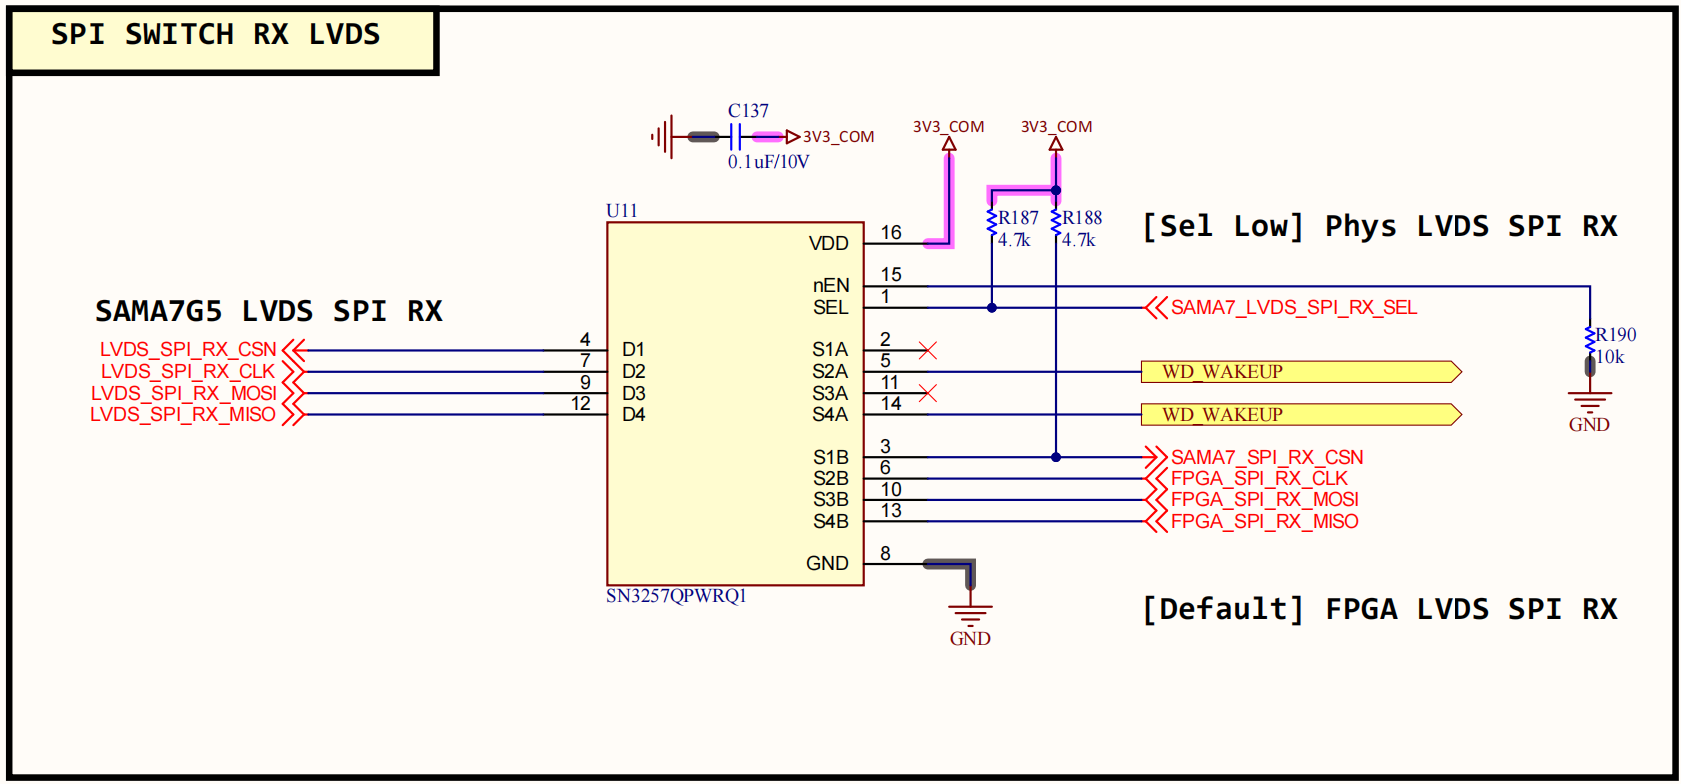
\includegraphics[width=0.9\textwidth]{picture/if/spi-sw-lvds-rx.png}
    \\caption{Sơ đồ nguyên lí khối SPI switch LVDS TX}
    \label{fig:if-spi-sw-lvds}
\end{figure}

\begin{figure}[H]
    \centering
    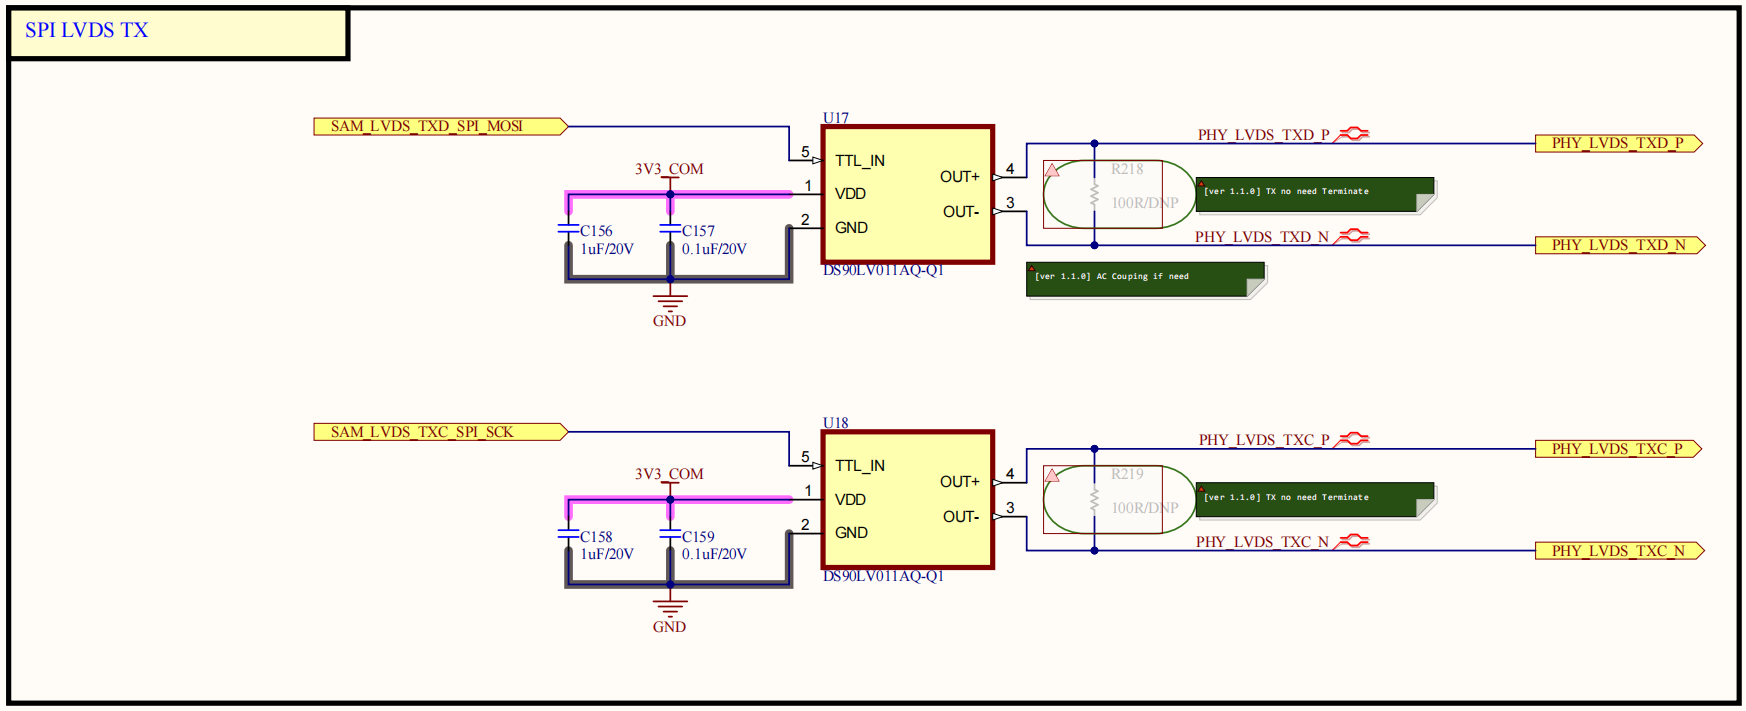
\includegraphics[width=0.9\textwidth]{picture/if/spi-lvds-tx.png}
    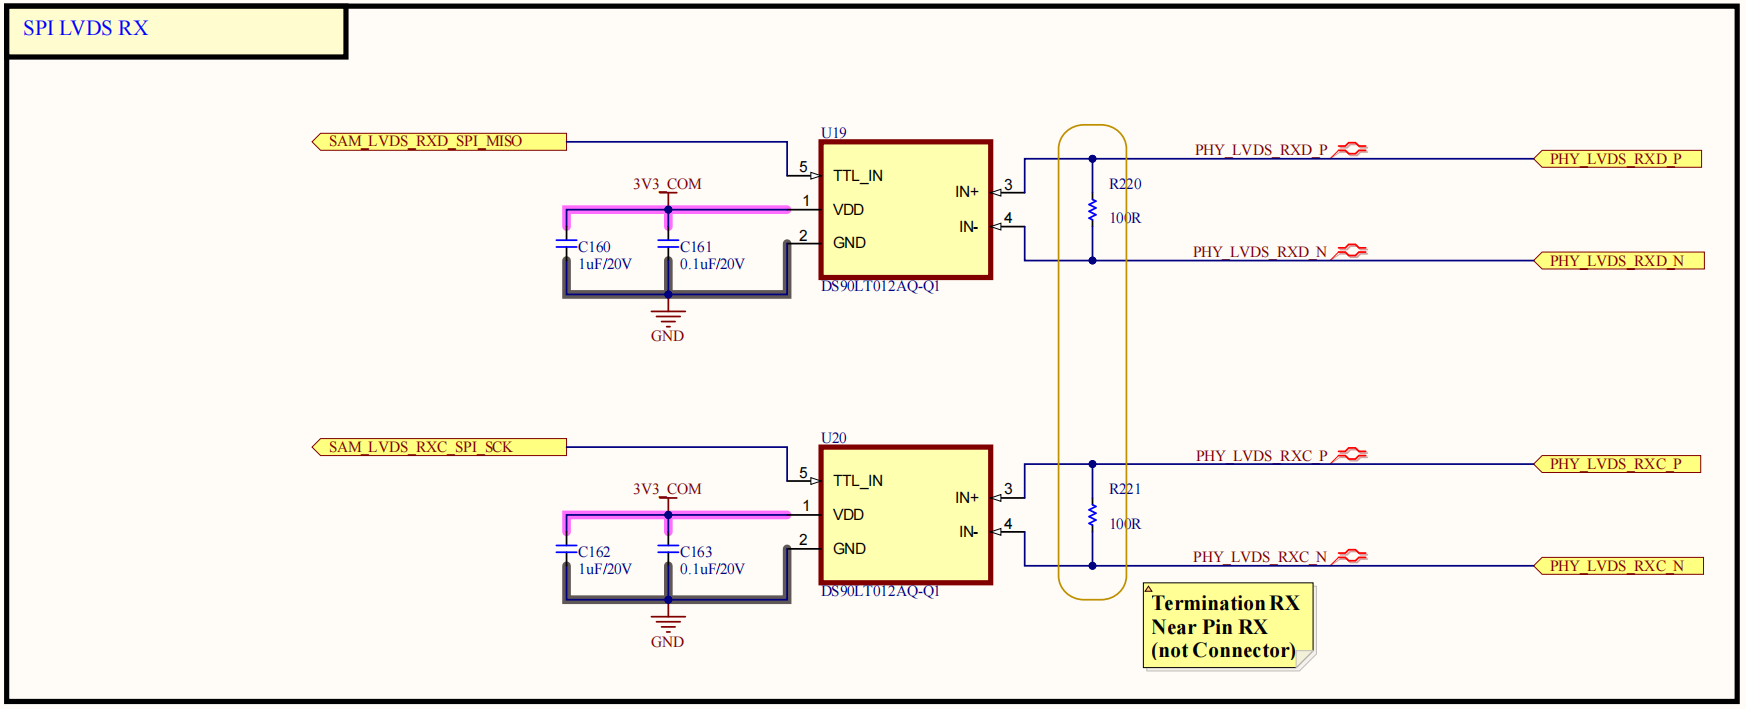
\includegraphics[width=0.9\textwidth]{picture/if/spi-lvds-rx.png}
    \\caption{Sơ đồ nguyên lí khối SPI LVDS}
    \label{fig:if-spi-lvds}
\end{figure}

Trong thiết kế, IC dùng cho việc chuyển đổi dữ liệu phát từ tín hiệu đơn sang LVDS là DS90LV011AQ-Q1 driver, còn IC dùng cho việc thu dữ liệu chuyển từ tín hiệu điện LVDS sang tín hiệu đơn là DS90LT012AQ-Q1 receiver.

Ở dây được thiết kế gồm 2 cặp LVDS. 1 cặp với tín năng phát dữ liệu bao gồm tín hiệu dữ liệu và tín hiệu xung clock. Cặp còn lại sẽ là tín hiệu thu dữ liệu và xung clock.

Đối với bus phát dữ liệu, dùng IC DS90LV011AQ-Q1 để chuyển đổi ngõ vào thành dạng vi sai. Ngõ vào của driver là tín hiệu SPI MOSI và SPI CLK, ngõ ra là tín hiệu điện dạng vi sai (LVDS) từ 2 tín hiệu ngõ vào.  Hai driver này đóng vai trò là nguồn phát nên ở giữa mỗi cặp vi sai không nhất thiết phải có điện trở termination. Tín hiệu MOSI và CLK là ngõ ra của SPI SWITCH TX LVDS (lựa chọn giữa IC driver và FPGA về MPU).

Đối với bus thu dữ liệu, dùng IC DS90LT012AQ-Q1 để chuyển đổi từ tín hiệu LVDS về tín hiệu đơn. Ngõ vào của receiver là tín hiệu LVDS dữ liệu thu và LVDS clock, ngõ ra là tín hiệu SPI MISO và SPI CLK. Hai tín hiệu ngõ ra này sẽ kết nối với khối SPI SWITCH LVDS RX, từ đó có thể chọn một trong hai tín hiệu SPI (từ receiver hoặc FPGA) về MPU. Thiết kế receiver là vị trí thu nên ở cuối đường dây có trở termination 100R.

\begin{figure}[H]
    \centering
    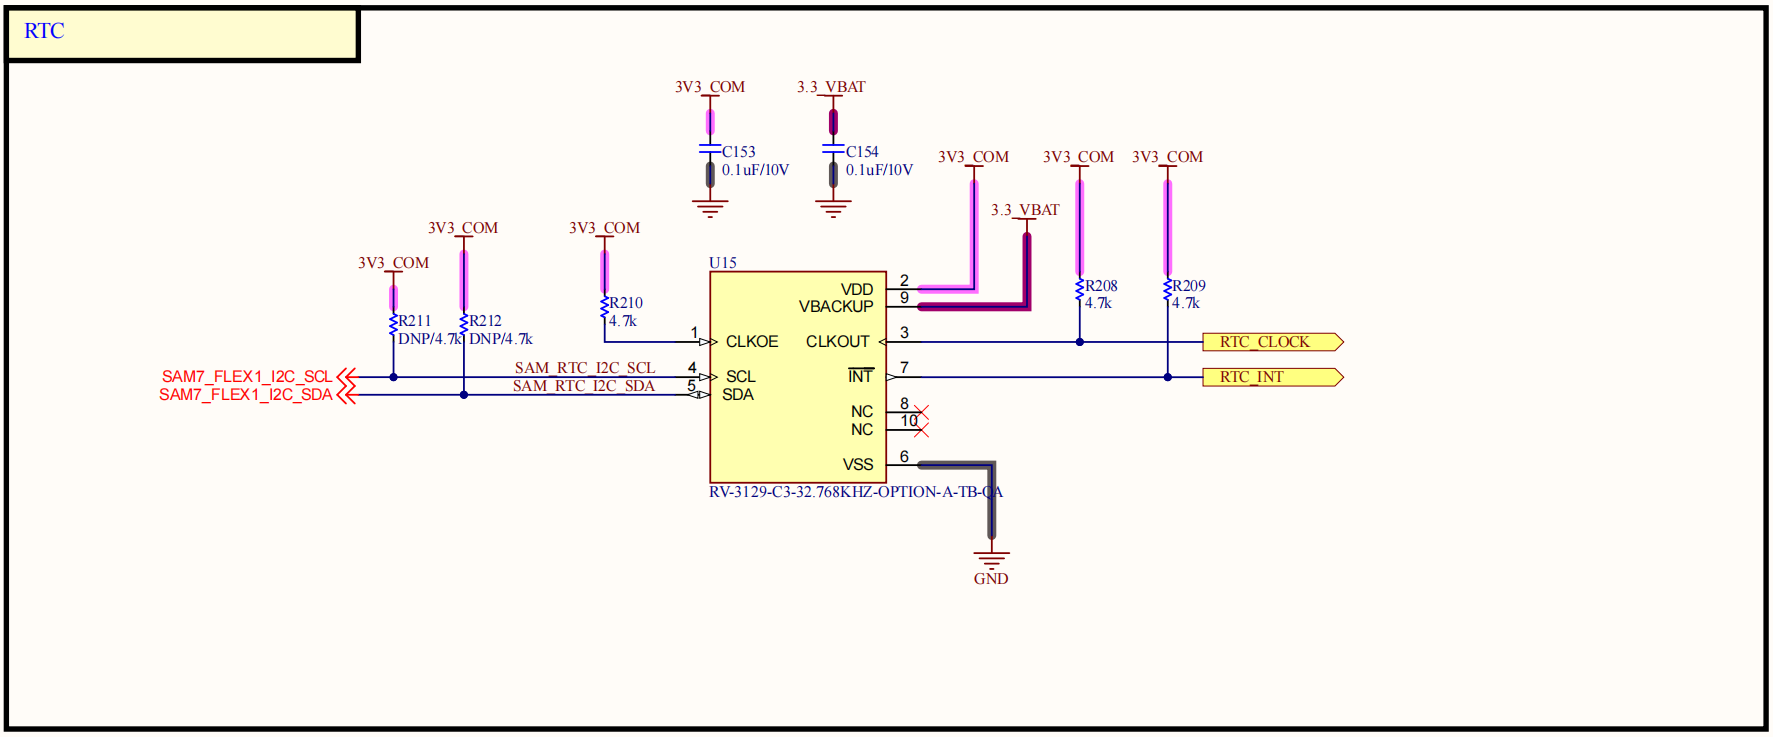
\includegraphics[width=1\textwidth]{picture/if/if-rtc.png}
    \\caption{Sơ đồ nguyên lí khối RTC}
    \label{fig:if-rtc}
\end{figure}

Thiết kế của RTC cũng tương tự như trên board EXP, tín hiệu giao tiếp với IC là I2C và các tín hiệu ra là RTC\_CLOCK và RTC\_INT.


\begin{figure}[H]
    \centering
    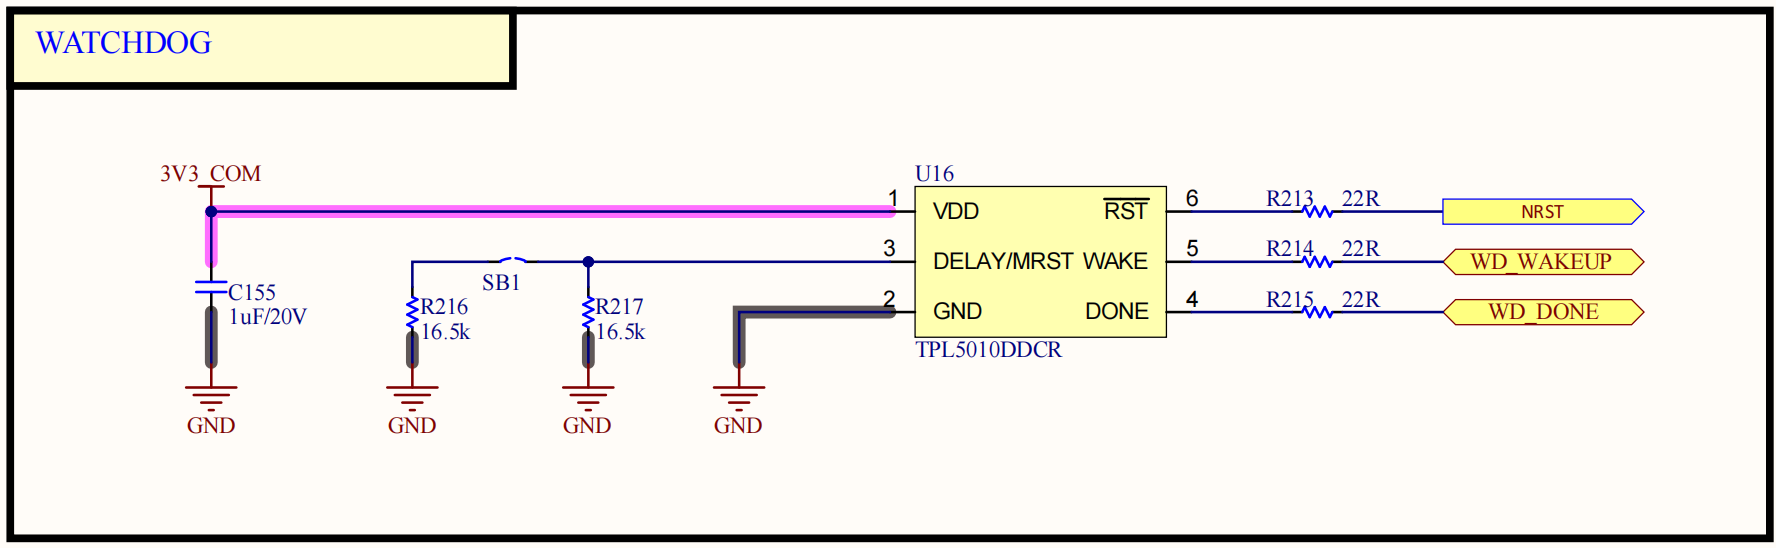
\includegraphics[width=1\textwidth]{picture/if/if-watchdog.png}
    \\caption{Sơ đồ nguyên lí khối watchdog}
    \label{fig:if-watchdog}
\end{figure}

Khối watchdog dùng TPL5010DDCR và cấu hình thời gian tương tự trên board EXP.

\begin{figure}[H]
    \centering
    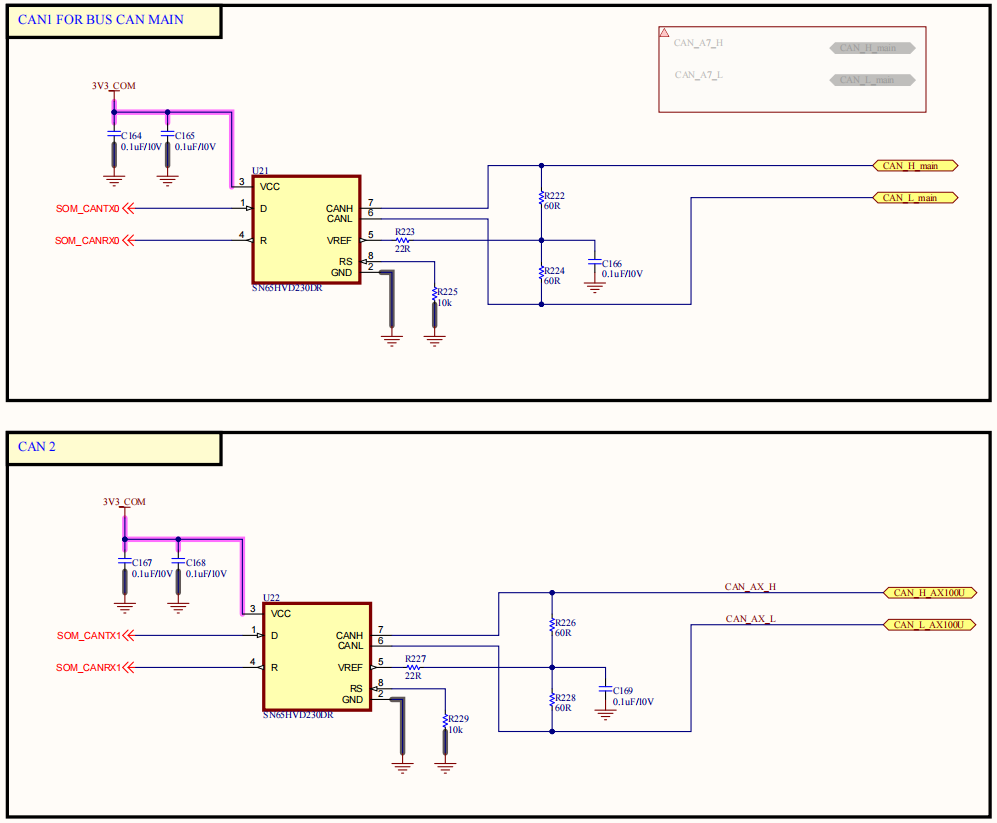
\includegraphics[width=1\textwidth]{picture/if/if-can.png}
    \\caption{Sơ đồ nguyên lí khối CAN}
    \label{fig:if-can}
\end{figure}

Thiết kế dùng 2 kênh CANTX/RX 0/1 từ MPU sang IC CAN transceiver SN65HVD230DR để chuyển thành tín hiệu vi sai trong bus CAN tương tự như thiết kế của EXP. Cả 2 ngõ ra của IC CAN đều kết nối chung vào một bus, kéo ra connector PC104 và connector cho GNSS OEM719A.

\begin{figure}[H]
    \centering
    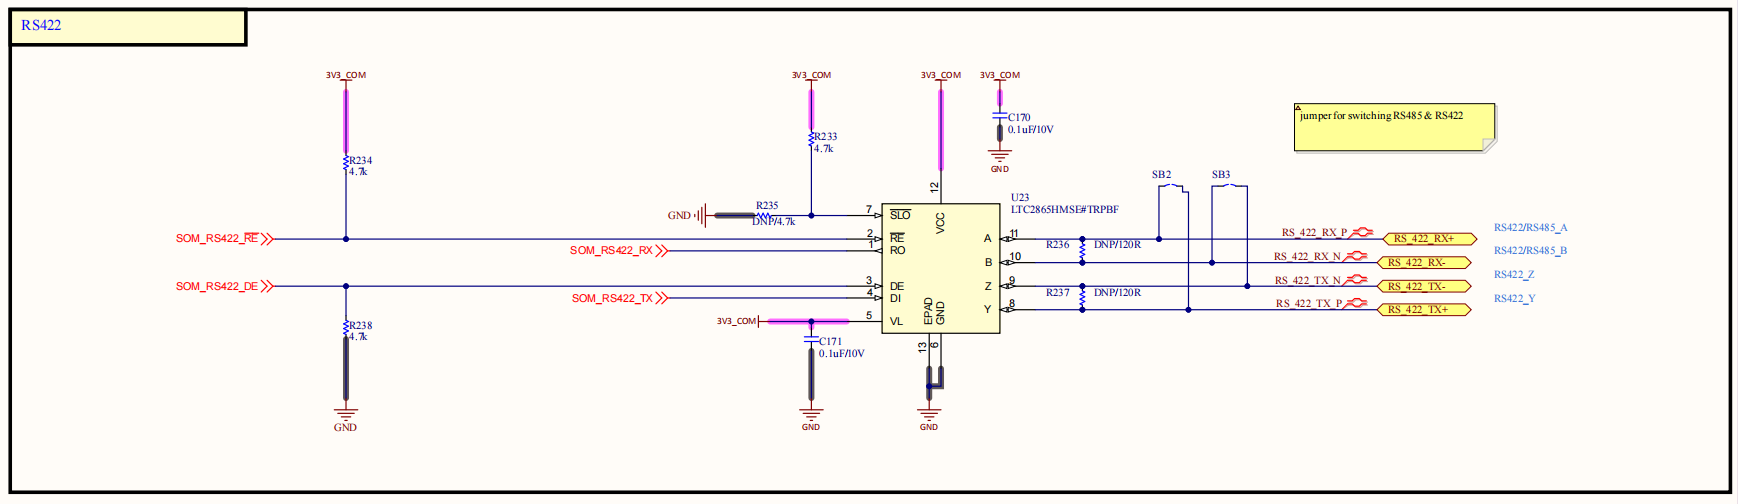
\includegraphics[width=1\textwidth]{picture/if/rs422.png}
    \\caption{Sơ đồ nguyên lí khối RS422}
    \label{fig:if-rs422}
\end{figure}

LTC2865HMSE\#TRPBF là bộ thu phát RS485/RS422 công suất thấp, có khả năng bảo vệ lỗi quá áp lên đến ±60V và dải điện áp chế độ chung mở rộng ±25V. Thiết bị hoạt động dựa trên nguyên lý chuyển đổi tín hiệu logic thành tín hiệu vi sai để truyền dẫn (và ngược lại) với tốc độ tối đa 20Mbps hoặc 250kbps (chế độ giảm nhiễu EMI), đồng thời tích hợp tính năng "failsafe" đảm bảo đầu ra bộ thu luôn ở mức logic 1 khi đường truyền bị hở, ngắn mạch hoặc không được điều khiển. Các tín hiệu kết nối chính bao gồm nguồn VCC (3V đến 5.5V), các chân dữ liệu logic DI/RO, chân điều khiển RE/DE, và các đường truyền vi sai A, B (cho kiểu Half-Duplex) hoặc Y, Z, A, B (cho kiểu Full-Duplex); riêng phiên bản LTC2865 có thêm chân VL để hỗ trợ giao diện logic điện áp thấp và chân SLO để điều khiển tốc độ biến thiên.

\begin{figure}[H]
    \centering
    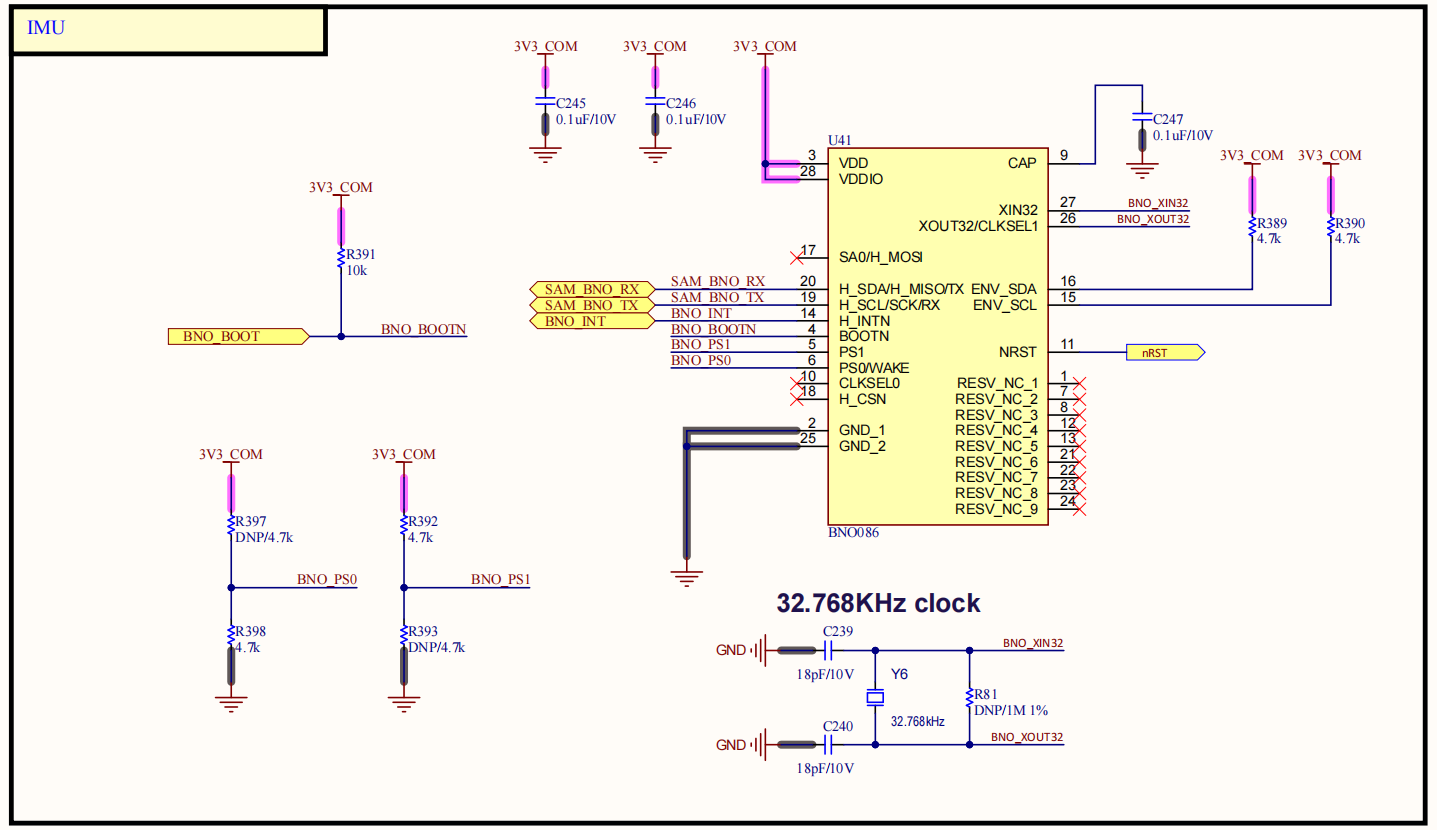
\includegraphics[width=1\textwidth]{picture/if/imu.png}
    \\caption{Sơ đồ nguyên lí khối IMU}
    \label{fig:if-imu}
\end{figure}

BNO08X (BNO085/BNO086) là cảm biến quán tính dạng SiP tích hợp gia tốc kế 3 trục, con quay hồi chuyển 3 trục, từ kế và vi điều khiển Cortex-M0+ chạy firmware SH-2/MotionEngine để xử lý hợp nhất cảm biến ngay trên chip. Nhờ đó, linh kiện có thể xuất trực tiếp các đại lượng như gia tốc đã hiệu chuẩn, vận tốc góc, vector quay (quaternion), gravity và các đầu ra phân loại chuyển động mà không cần host xử lý hợp nhất dữ liệu mức thấp. Về giao tiếp, BNO08X hỗ trợ nhiều chuẩn kết nối host gồm I2C, SPI, UART-SHTP và UART-RVC, thuận tiện cho tích hợp với cả MCU và SoC. Datasheet cũng nêu khả năng xuất dữ liệu theo tốc độ lấy mẫu cấu hình được, có dấu thời gian cho report và chế độ gyro rotation vector độ trễ thấp đến 1~kHz cho các ứng dụng AR/VR hoặc điều khiển thời gian thực.

\begin{figure}[H]
    \centering
    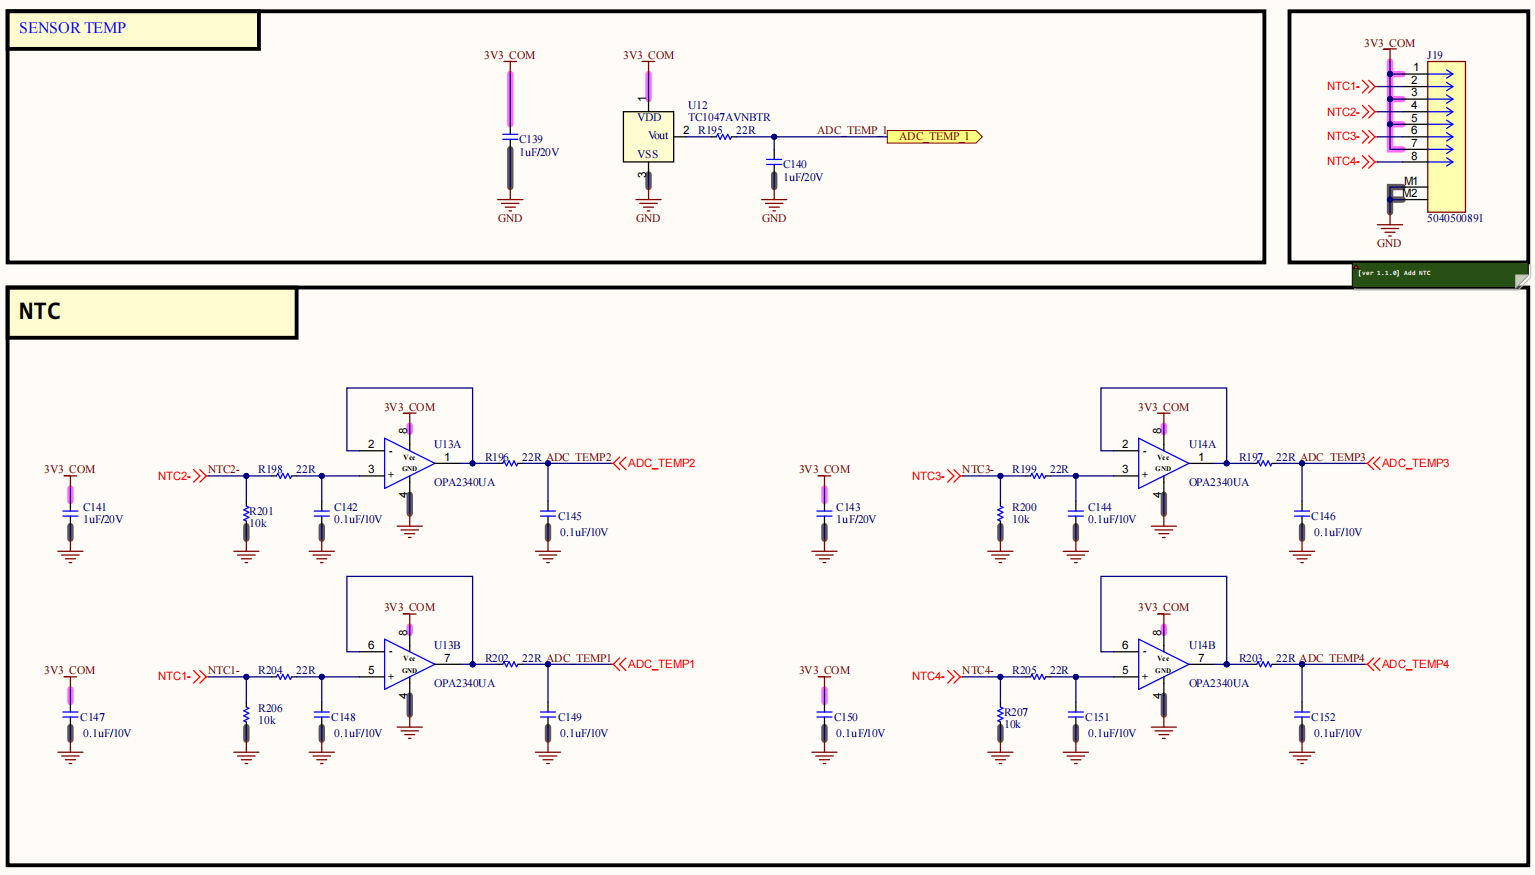
\includegraphics[width=1\textwidth]{picture/if/temp.png}
    \\caption{Sơ đồ nguyên lí khối temp}
    \label{fig:if-temp}
\end{figure}

Sử dụng một cảm biến nhiệt độ đơn giản onboard TC1047AVNBTR để theo dõi nhiệt trên board và các IC NTC nối connector để linh hoạt dùng NTC ở các vị trí mong muốn. Các thiết kế NTC dùng như trên board EXP nhưng số lượng lúc này chỉ còn 4 NTC để phù hợp với số lượng chân trên connector và kiểm tra nhiệt đơn giản do việc điều khiển nhiệt không phải là chức năng chính của board IF. Việc cân chỉnh dãy tín hiệu đọc về từ NTC cũng được tính toán bởi phần mềm.

\begin{figure}[H]
    \centering
    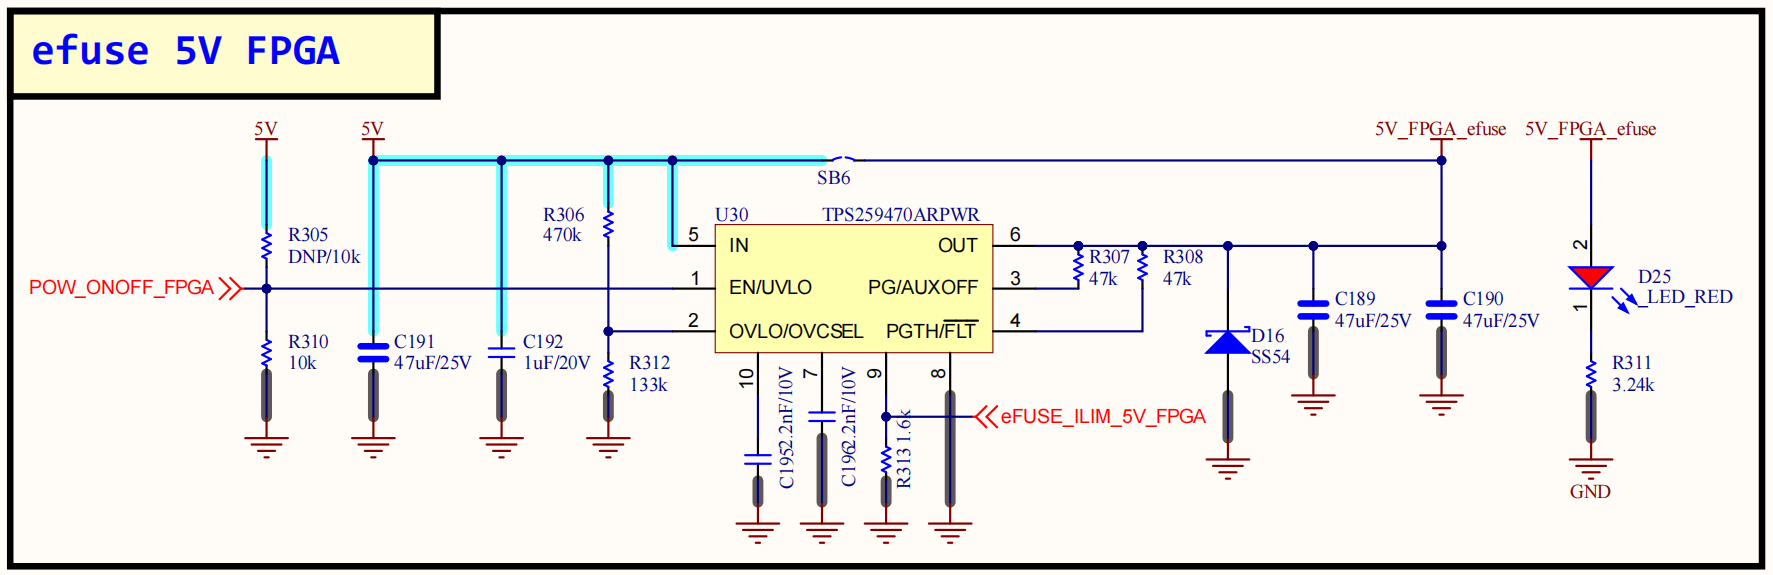
\includegraphics[width=0.8\textwidth]{picture/if/efuse-5v.png}
    \caption{eFuse 5V cho nguồn FPGA}
    \label{fig:tin-hieu-fpga}
\end{figure}

\begin{figure}[H]
    \centering
    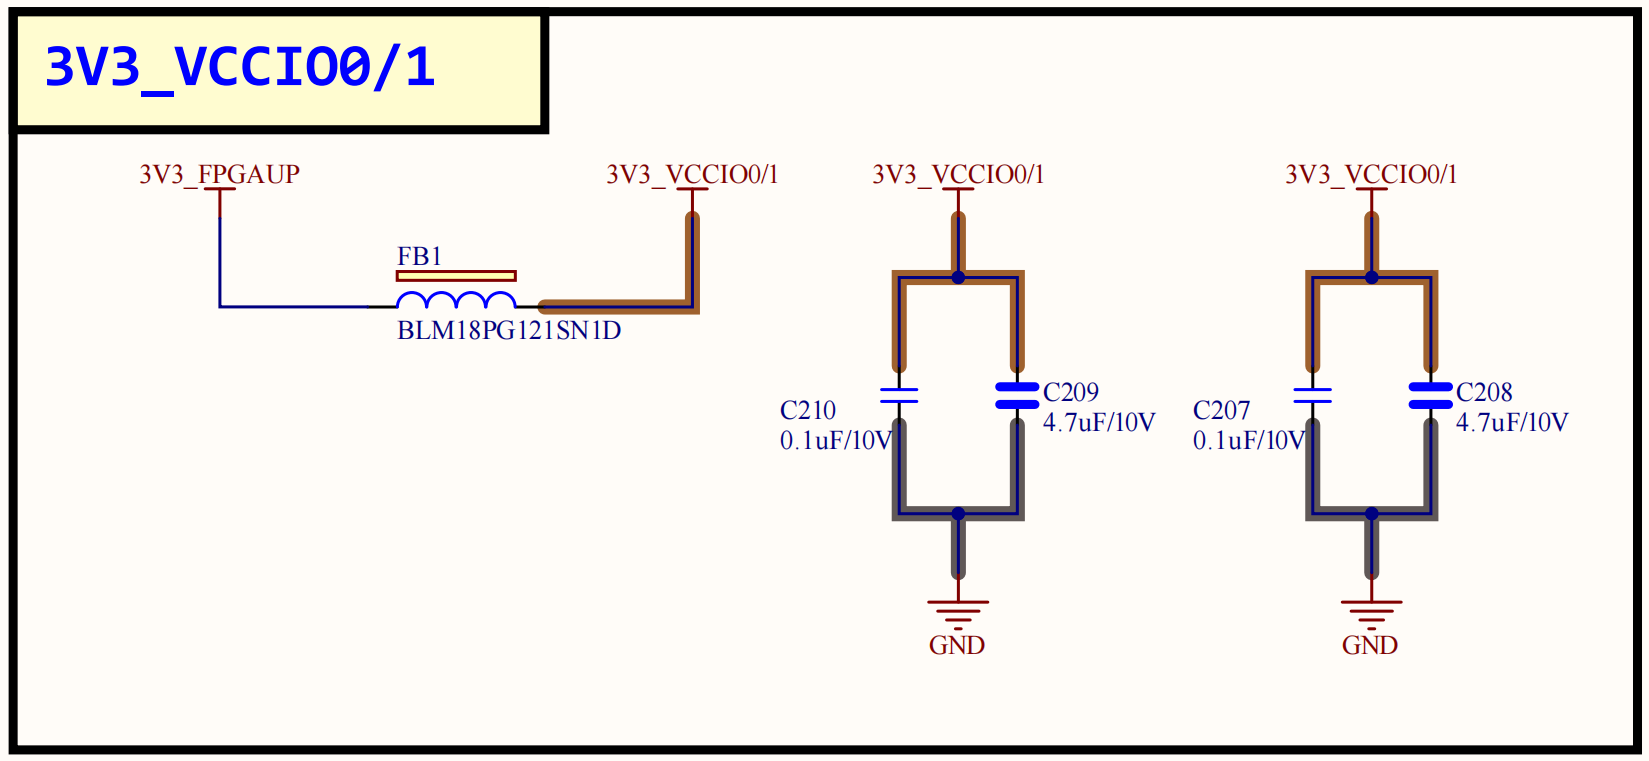
\includegraphics[width=0.6\textwidth]{picture/if/3v3-vccio01.png}
    \caption{Nguồn 3V3 cho IO0/1 của FPGA}
    \label{fig:fpga-3v3-io01}
\end{figure}

Các bank IO0/1 của FPGA sử dụng nguồn cấp 3V3, ở đây ta lọc tín hiệu 3V3 bằng 1 cuộn ferrite và tụ lọc.

\begin{figure}[H]
    \centering
    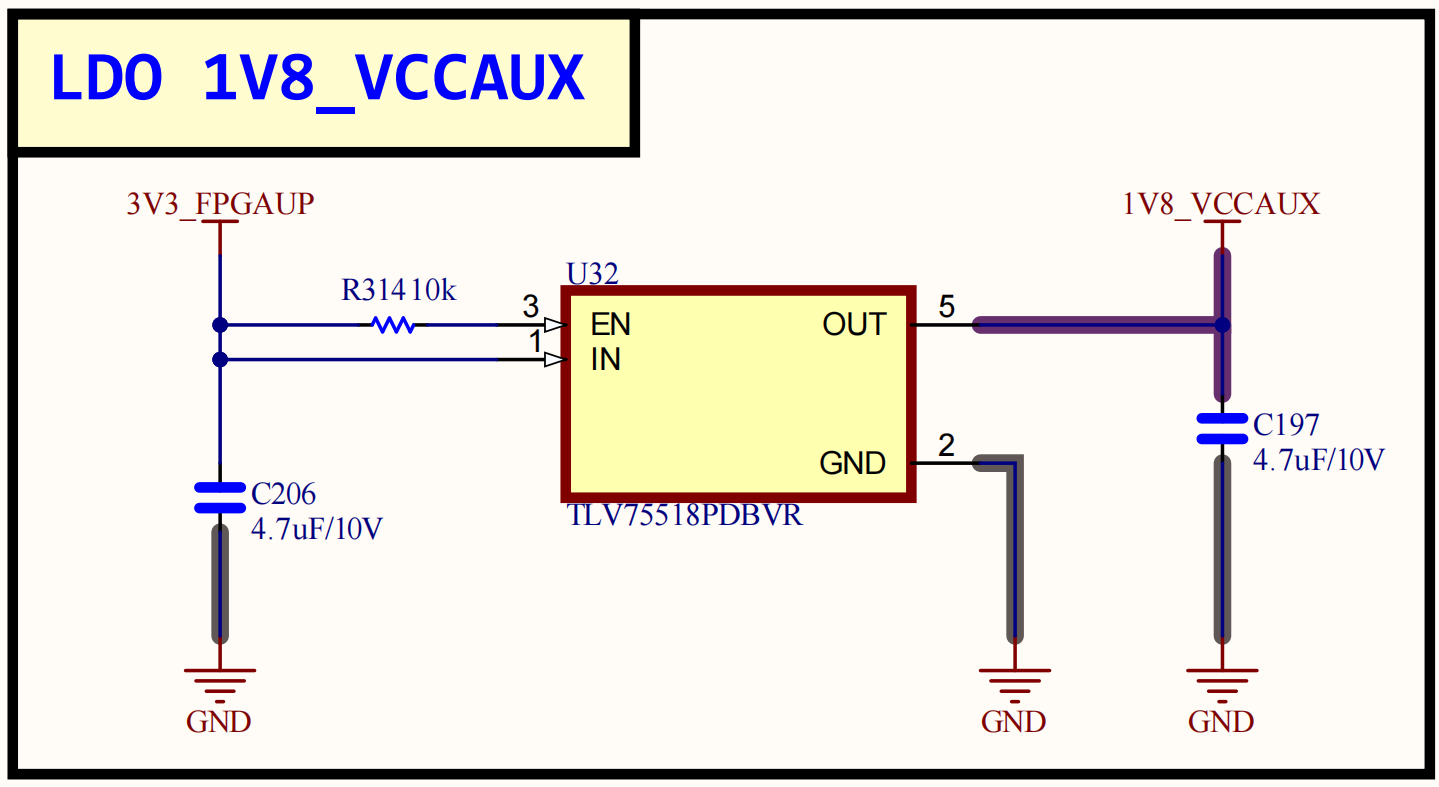
\includegraphics[width=0.6\textwidth]{picture/if/ldo-1v8-vccaux.png}
    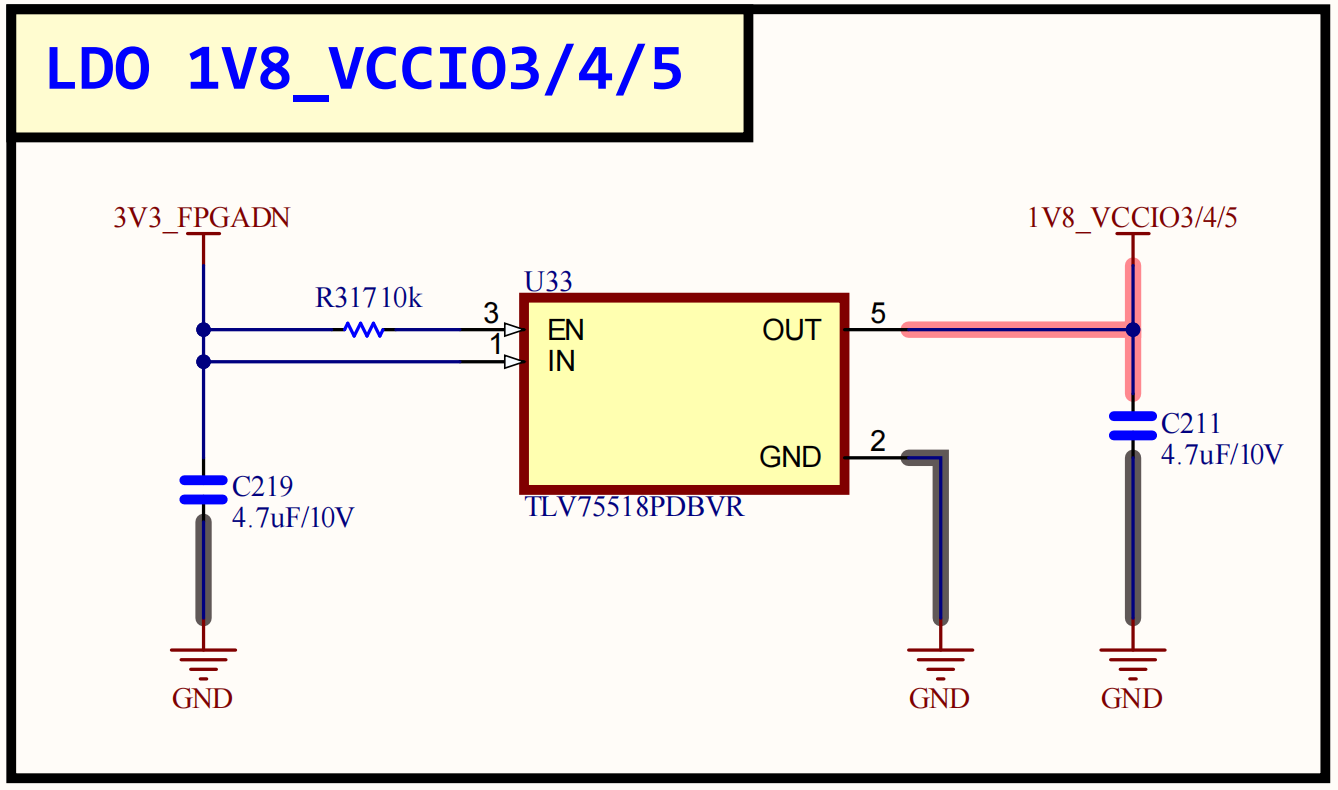
\includegraphics[width=0.6\textwidth]{picture/if/ldo-1v8-vccio345.png}
    \caption{LDO 1V8}
    \label{fig:fpga-ldo-1v8}
\end{figure}

Một số IO trên FPGA cần được cấp nguồn 1V8, ví dụ như các IO của bank 3, 4, 5 và nguồn AUX.

\begin{figure}[H]
    \centering
    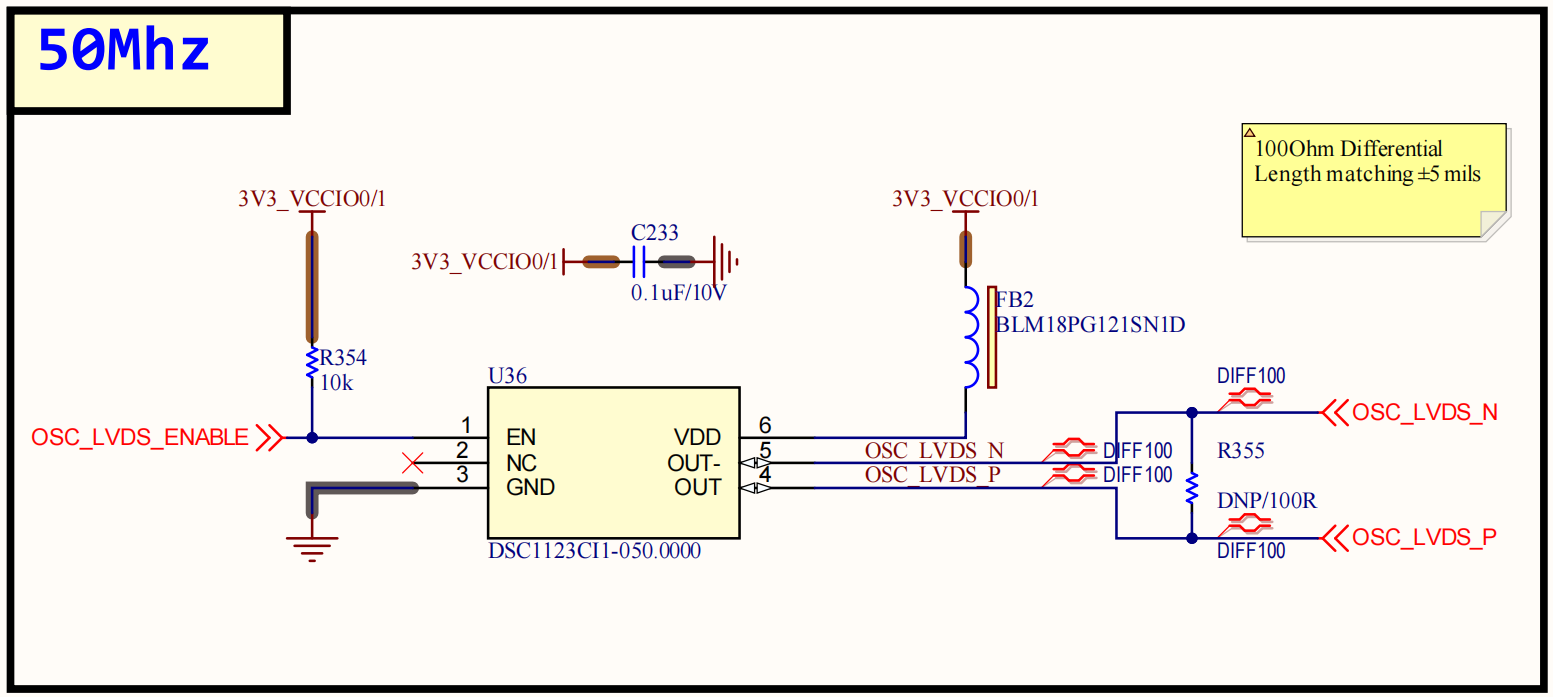
\includegraphics[width=0.6\textwidth]{picture/if/50mhz-fpga.png}

    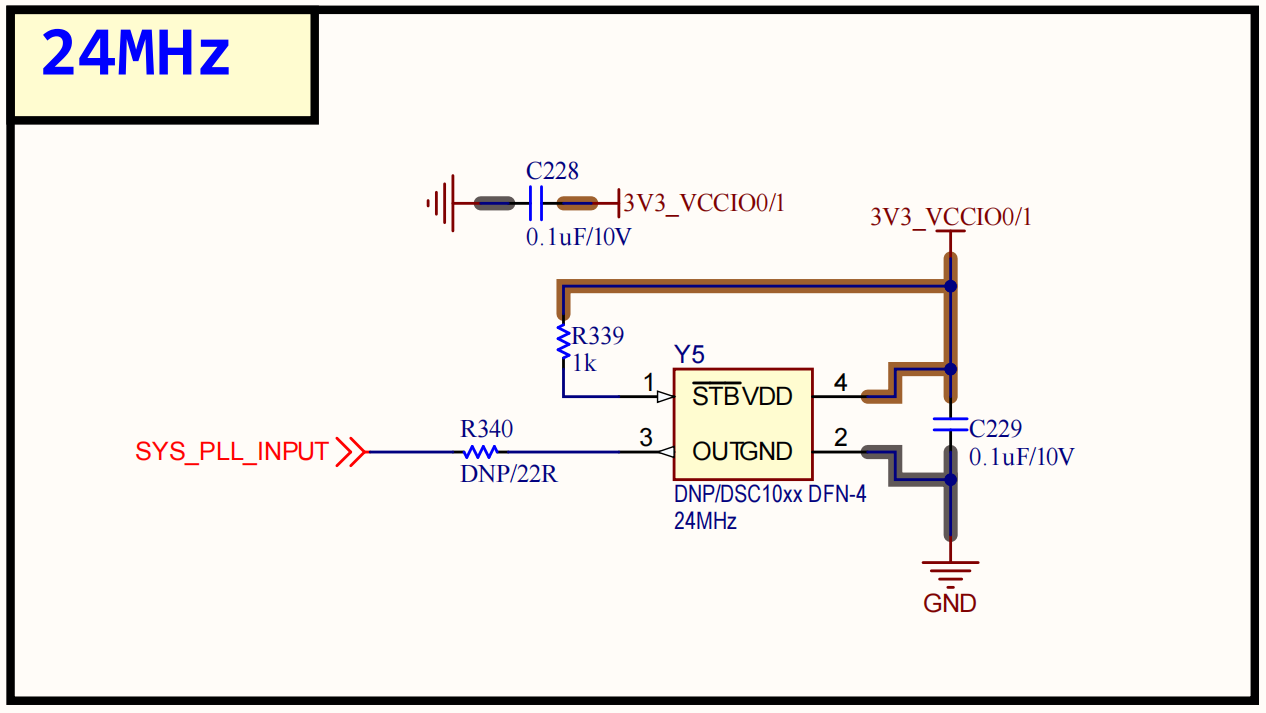
\includegraphics[width=0.6\textwidth]{picture/if/24mhz-fpga.png}
    \\caption{Sơ đồ nguyên lí khối tạo dao động cho FPGA}
    \label{fig:clock-fpga}
\end{figure}

FPGA sử dụng một nguồn LVDS tốc độ cao với tần số xung clock 50MHz và một bộ dao động cấp tần số 24MHz.

\begin{figure}[H]
    \centering
    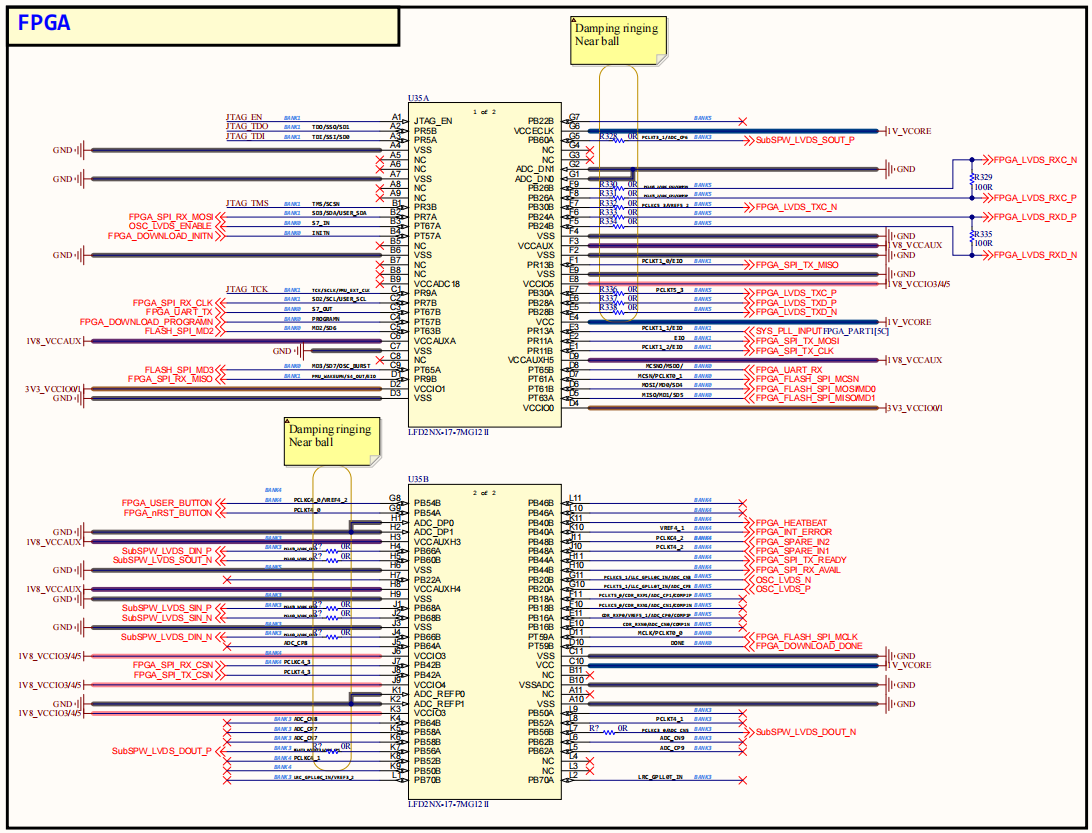
\includegraphics[width=1\textwidth]{picture/if/fpga.png}
    \caption{Tín hiệu trên FPGA}
    \label{fig:tin-hieu-fpga}
\end{figure}

Các nhóm tín hiệu chính sử dụng trên FPGA bao gồm: tín hiệu UART giao tiếp trực tiếp giữa FPGA và core MPU, tín hiệu SPI/QSPI để FPGA giao tiếp với IC FLASH trên board, các tín hiệu ra connector LVDS chính và phụ.


\begin{figure}[H]
    \centering
    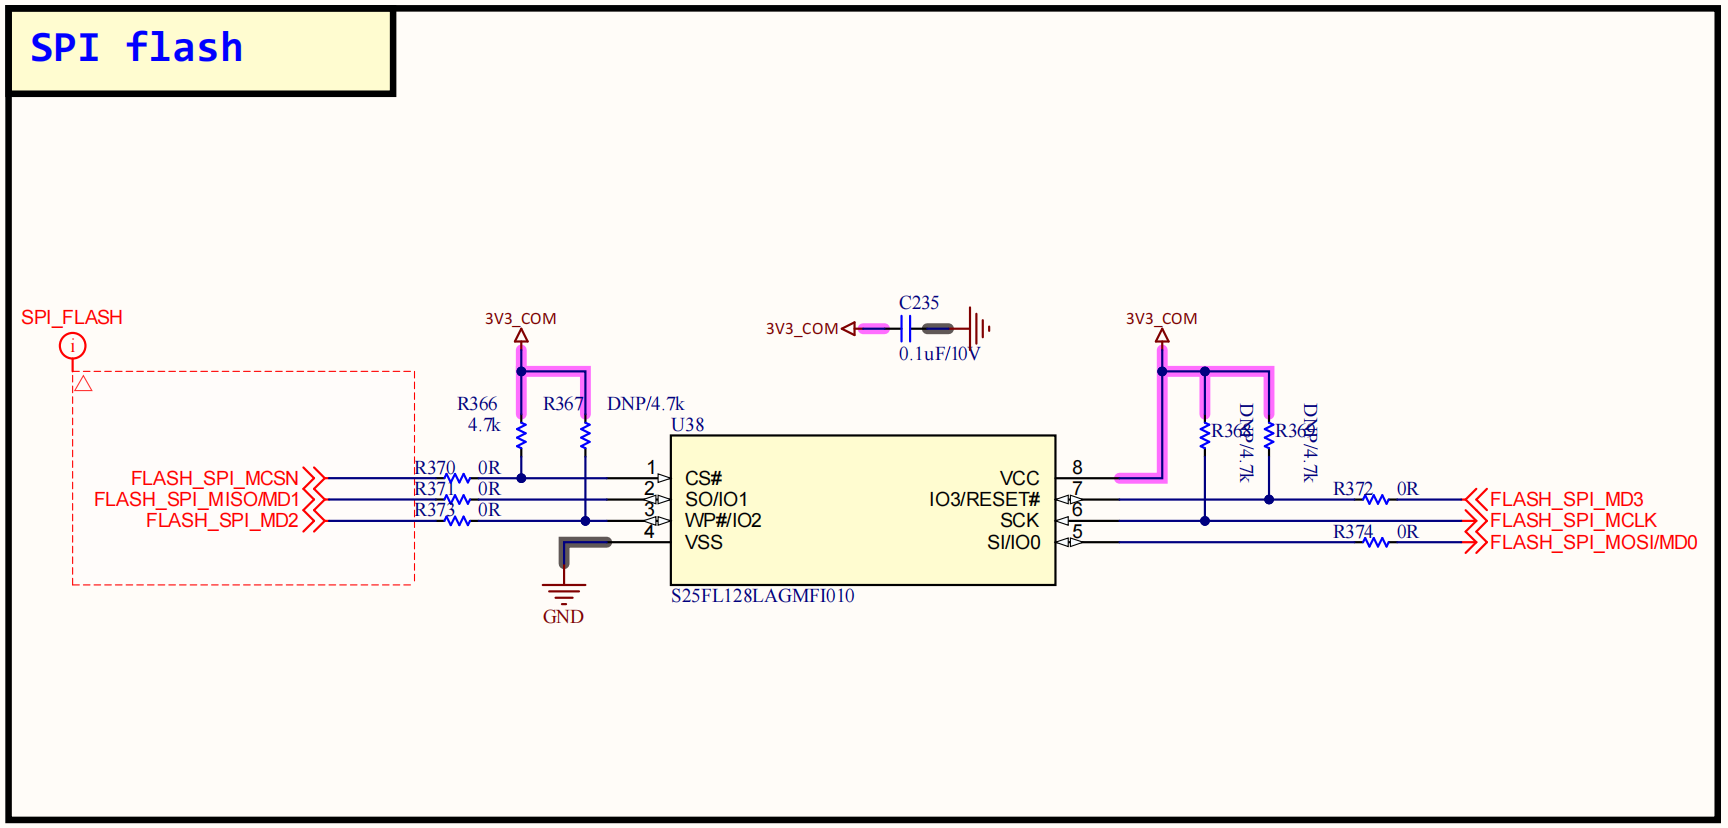
\includegraphics[width=1\textwidth]{picture/if/fpga-spi-flash.png}
    \caption{IC FLASH SPI FPGA - MPU}
    \label{fig:if-fpga-spi-flash}
\end{figure}

Khối SPI Flash sử dụng dòng S25FL-L (S25FL128L/S25FL256L), là bộ nhớ NOR Flash không bay hơi (non-volatile) dùng công nghệ floating-gate, phù hợp cho lưu firmware, cấu hình và dữ liệu cần giữ sau khi mất nguồn. Dung lượng điển hình của họ này là 128 Mb (16 MB) hoặc 256 Mb (32 MB). Về giao tiếp, linh kiện hỗ trợ SPI đa I/O gồm chế độ SPI chuẩn (SIO), Dual I/O, Quad I/O, QPI và tùy chọn đọc DDR, cho phép mở rộng băng thông khi làm việc với FPGA/MCU. Theo bảng hiệu năng của datasheet, tốc độ đọc tối đa đạt khoảng 66 MB/s ở chế độ DDR Quad Read (xung 66 MHz), trong khi tốc độ lập trình trang điển hình khoảng 854 KB/s; kiến trúc ghi theo trang 256 byte và xóa theo sector/block (4 KB, 32 KB, 64 KB hoặc xóa toàn chip) đáp ứng linh hoạt cho cả cập nhật mã và lưu dữ liệu hệ thống.


\begin{figure}[H]
    \centering
    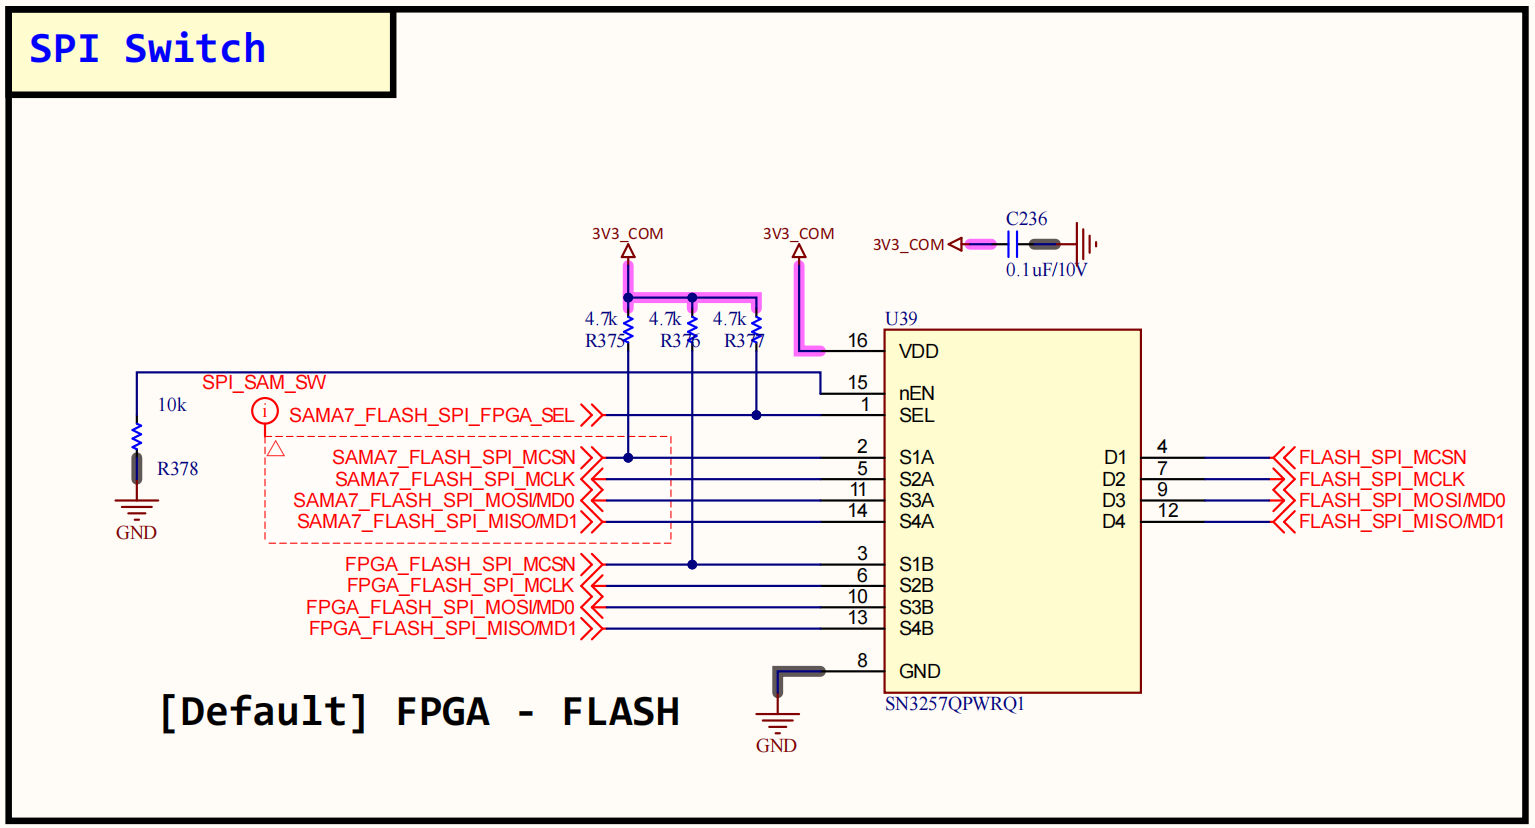
\includegraphics[width=1\textwidth]{picture/if/spi-sw.png}
    \caption{Sơ đồ nguyên lí khối SPI SWITCH giữa MPU và FPGA}
    \label{fig:if-spi-sw}
\end{figure}

SN3257-Q1 là bộ chuyển mạch CMOS 4 kênh, cấu hình 2:1 (SPDT), thường được dùng để đa hợp các giao thức như SPI, I2S. Thiết bị hoạt động dựa trên chân EN mức thấp để kích hoạt đồng thời các kênh và chân SEL để lựa chọn đường dẫn giữa các cặp chân nguồn (SxA, SxB) với chân máng (Dx) tương ứng. Các tín hiệu kết nối bao gồm 8 cổng nguồn, 4 cổng máng hỗ trợ truyền dẫn analog và digital hai chiều, cùng các chân điều khiển logic tương thích mức 1.8V. Ưu điểm của linh kiện là băng thông 2 GHz, độ trễ lan truyền 78 ps, tích hợp sẵn điện trở kéo xuống 6 MΩ, đi kèm tính năng Fail-safe logic và Powered-off protection (bảo vệ khi mất nguồn) lên đến 3.6V

SPI switch đóng vai trò quản lí tài nguyên dùng chung giữa MPU và FPGA, tài nguyên ở đây là IC SPI FLASH. SPI switch có ngõ vào là 2 kênh tín hiệu SPI của MPU và của FPGA. Tín hiệu ngõ ra để kết nối với SPI FLASH sẽ được chọn một trong hai bus ngõ vào này bằng chân SEL, chân SEL này được điều khiển bởi MPU. MPU là phần tử đóng vai trò cho phép MPU hay FPGA giao tiếp với SPI FLASH để đảm bảo tại một thời điểm chỉ có một phần tử được truy xuất đến SPI FLASH, đều này đảm bảo dữ liệu được toàn vẹn và không gây xung đột dữ liệu.

\subsection{Board phát năng lượng ánh sáng - LASER}
\label{subsec:sche-board-phat-laser}

\begin{figure}[H]
    \centering
    \begin{minipage}{0.49\textwidth}
        \centering
        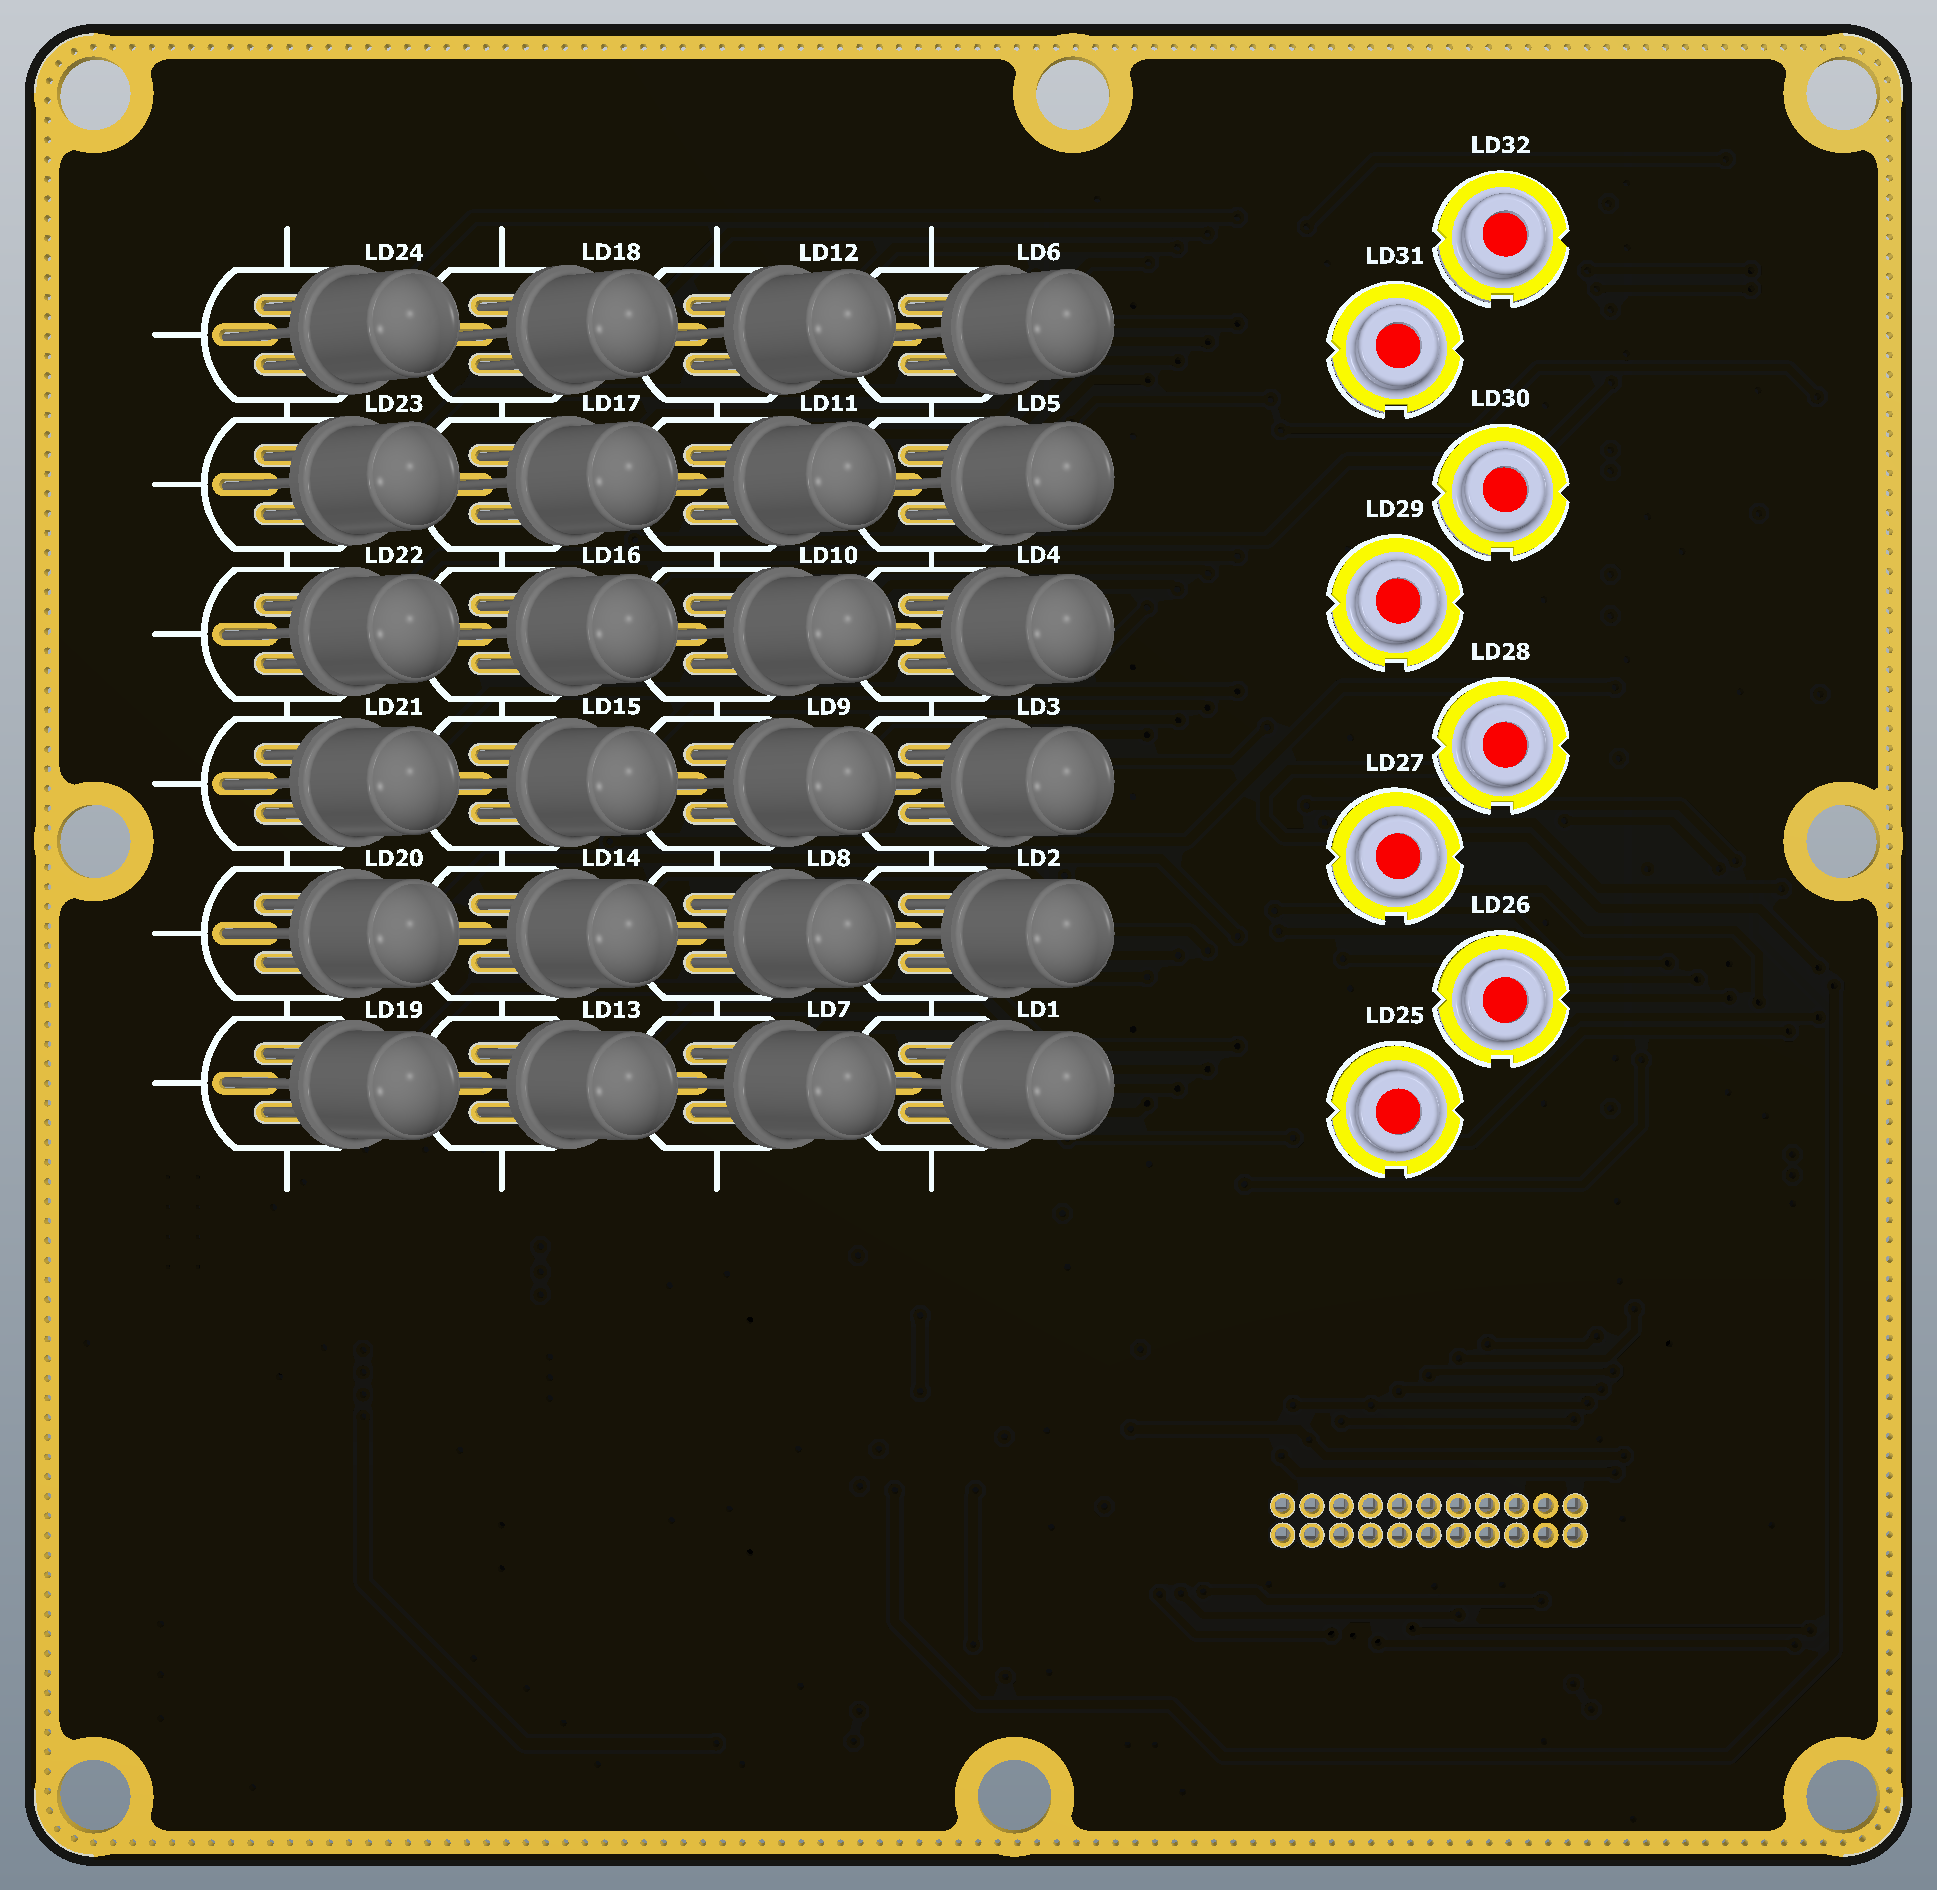
\includegraphics[width=\textwidth]{picture/laser/Satellite_4U_Laser_Int_Ext_V100.png}
        Mặt trên
    \end{minipage}
    \hfill
    \begin{minipage}{0.49\textwidth}
        \centering
        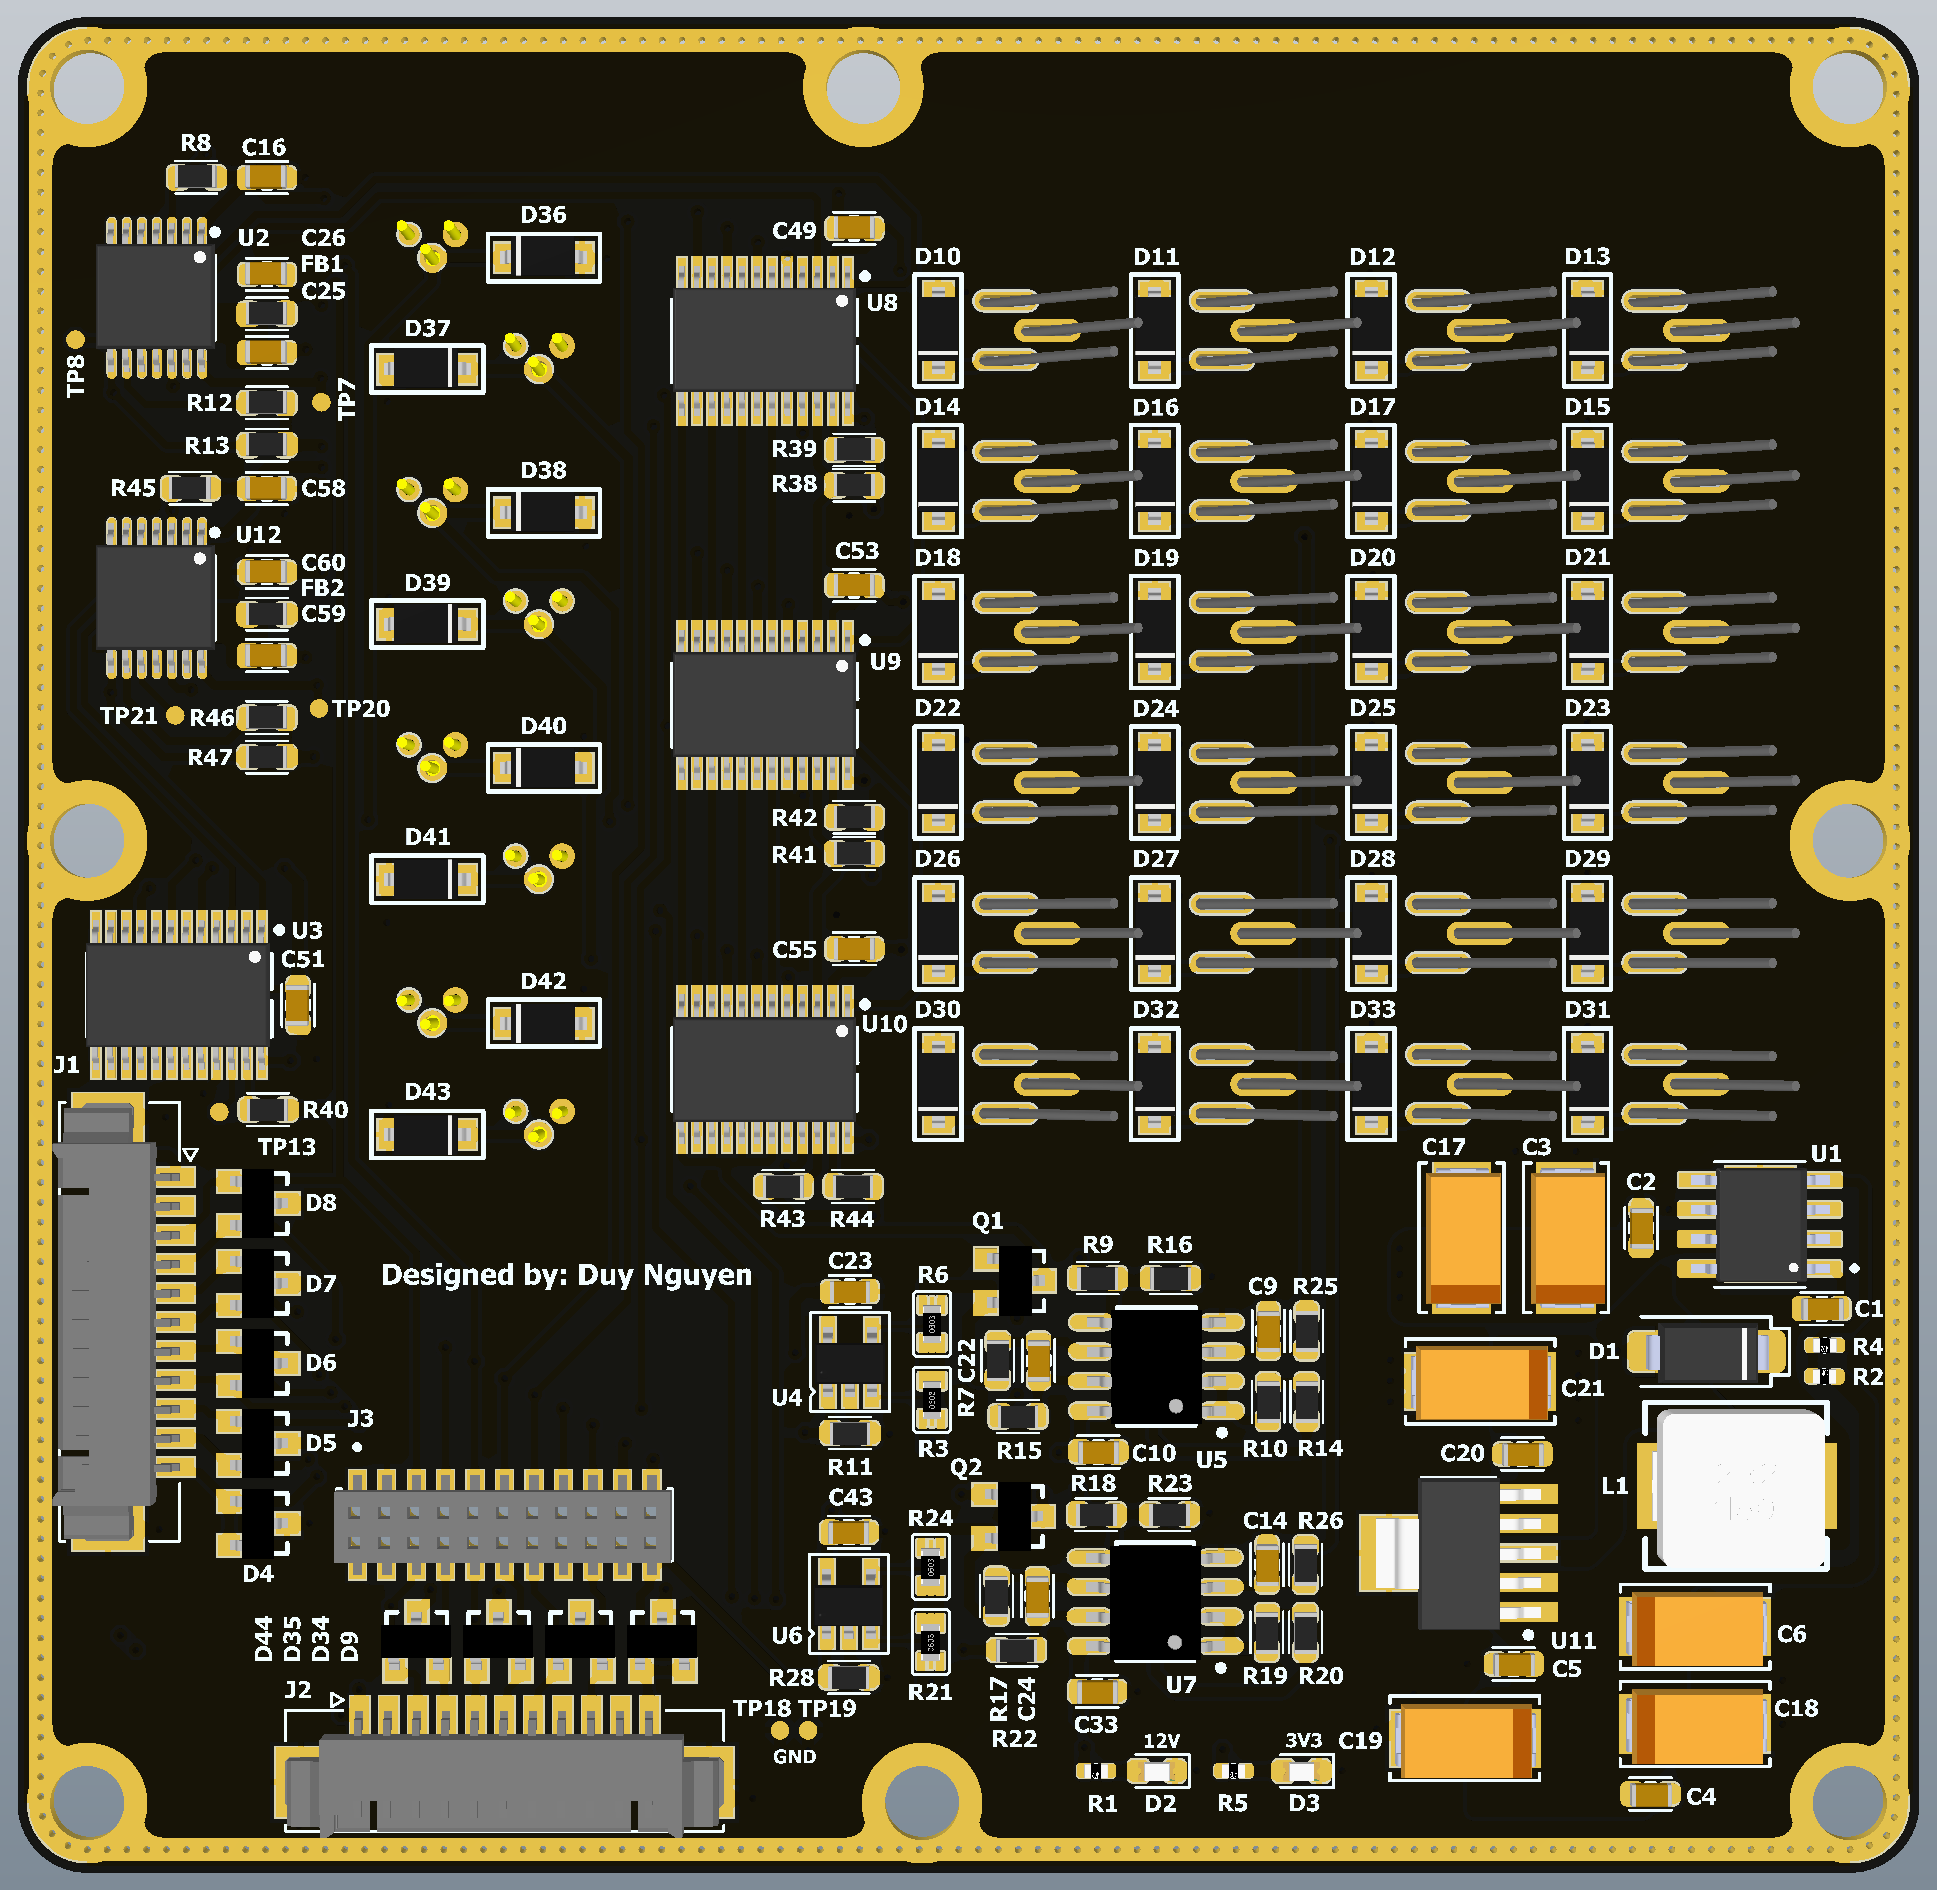
\includegraphics[width=\textwidth]{picture/laser/Satellite_4U_Laser_Int_Ext_V100-bot.png}
        Mặt dưới
    \end{minipage}
    \caption{PCB board LASER DIODE}
    \label{fig:laser-pcb-board}
\end{figure}

\subsubsection{Tính toán lý thuyết thiết kế mạch nguồn dòng}
\label{subsec:tinh-toan-nguon-dong}

\subsubsection{Mô phỏng nguyên lí mạch nguồn dòng}
\label{subsec:simulate-current-source}

Sử dụng phần mềm TINA-TI để mô phỏng nguồn dòng trong thiết kế để từ đó có thể lựa chọn những giá trị linh kiện phù hợp. Do board LASER đang sử dụng opamp OPAx192 thuộc linh kiện của nhà sản xuất TI nên sử dụng phần mềm mô phỏng của chính nhà phân phối để đảm bảo mô phỏng được kết quả tốt nhất.

\begin{figure}[H]
    \centering
    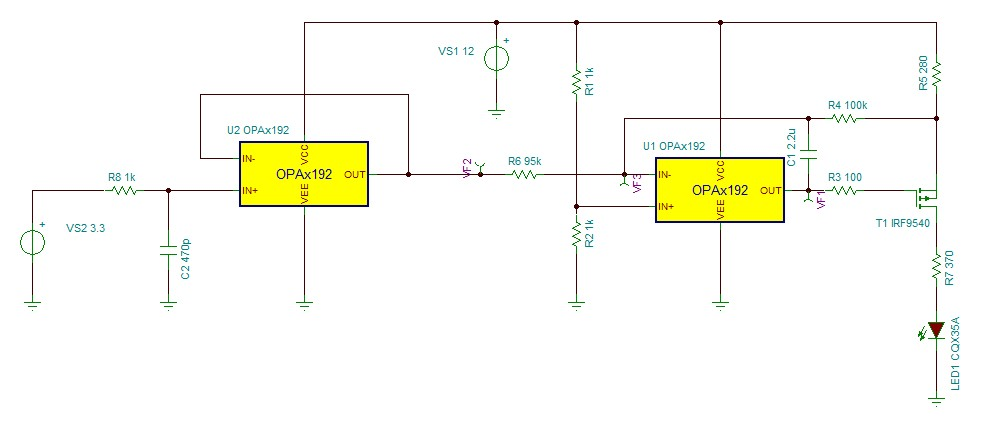
\includegraphics[width=0.9\textwidth]{picture/laser/simulate-current-int.JPG}
    \caption{Sơ đồ mô phỏng nguồn dòng cho internal laser}
    \label{fig:laser-simulate-current-int}
\end{figure}

Mạch mô phỏng bao gồm 2 tầng opamp. Tầng đầu tiên là tầng mạch đệm có thêm bộ lọc để triệt nhiễu ngõ vào và bảo đảm tách rời khỏi tầng opamp thứ hai. Tầng thứ hai là tầng chính để thực hiện mạch chuyển đổi điện áp sang dòng điện (V-I converter). Tín hiệu ngõ vào có dải điện áp từ 0 đến 3.3V.

Dựa vào công thức tính nguồn dòng:
$
I_{source} = \frac{V_{cc} - V_{s}}{R_{5}}
$

Ở đây khi mô phỏng và tính toán, dòng mong muốn khoảng 12\,mA, do đó chọn giá trị điện trở shunt; trong thiết kế $\R_{shunt} = 280\,\Omega&.

Do sụt áp trên laser internal OPV302 theo datasheet là tối đa khoảng 2.2V, với dòng thiết kế 12\,mA nên giả sử trong mạch mô phỏng thay OPV302 bằng điện trở có giá trị nhỏ hơn ngưỡng compliance voltage và cũng thỏa điều kiện rơi áp trên laser OPV312 khi có dòng chạy qua.


\begin{figure}[H]
    \centering
    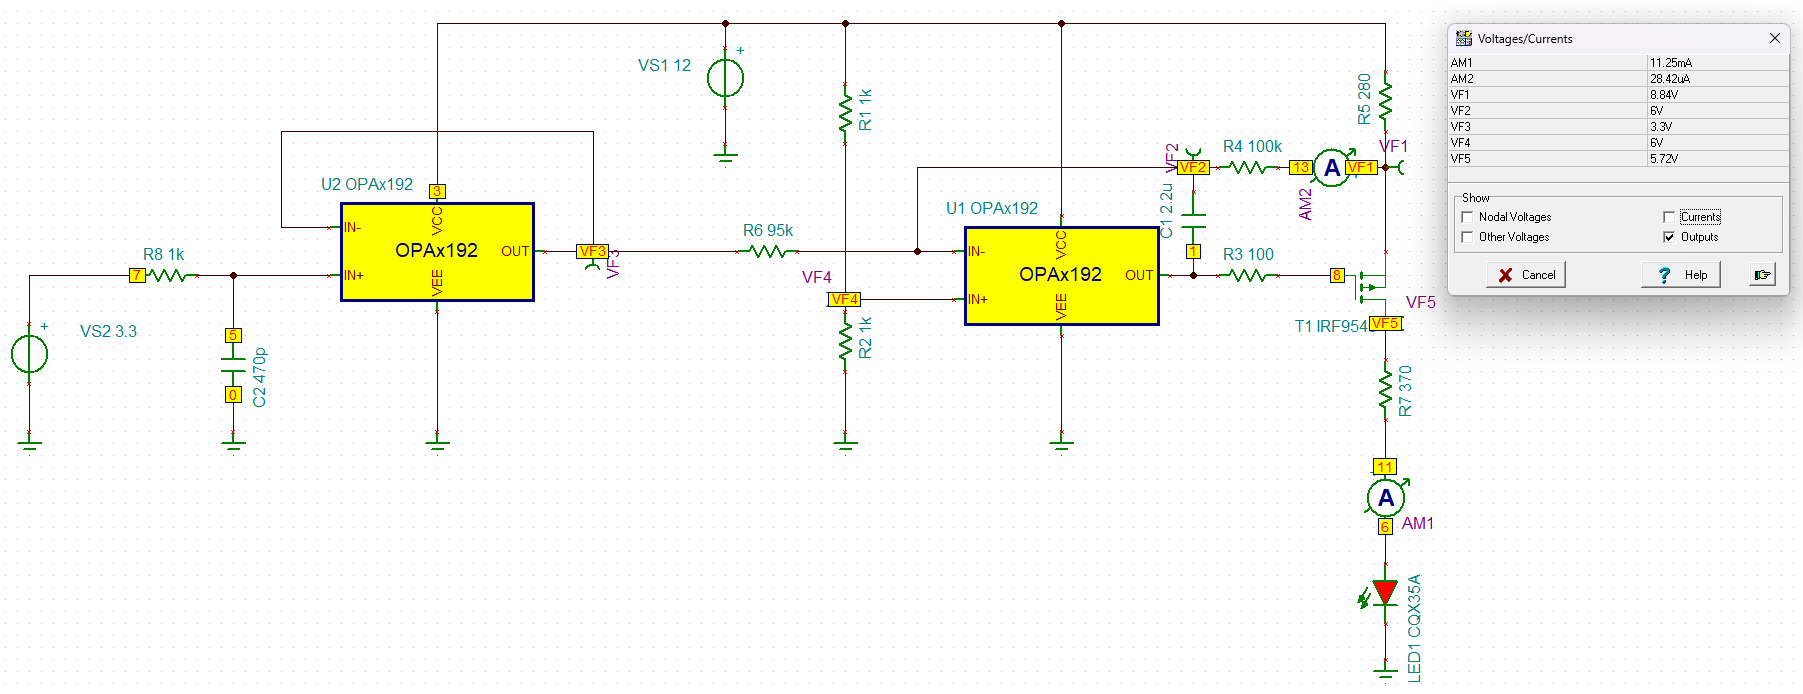
\includegraphics[width=0.9\textwidth]{picture/laser/current-int-dc-table.png}
    \caption{Bảng giá trị mô phỏng nguồn dòng internal}
    \label{fig:laser-current-int-dc-table}
\end{figure}

\begin{figure}[H]
    \centering
    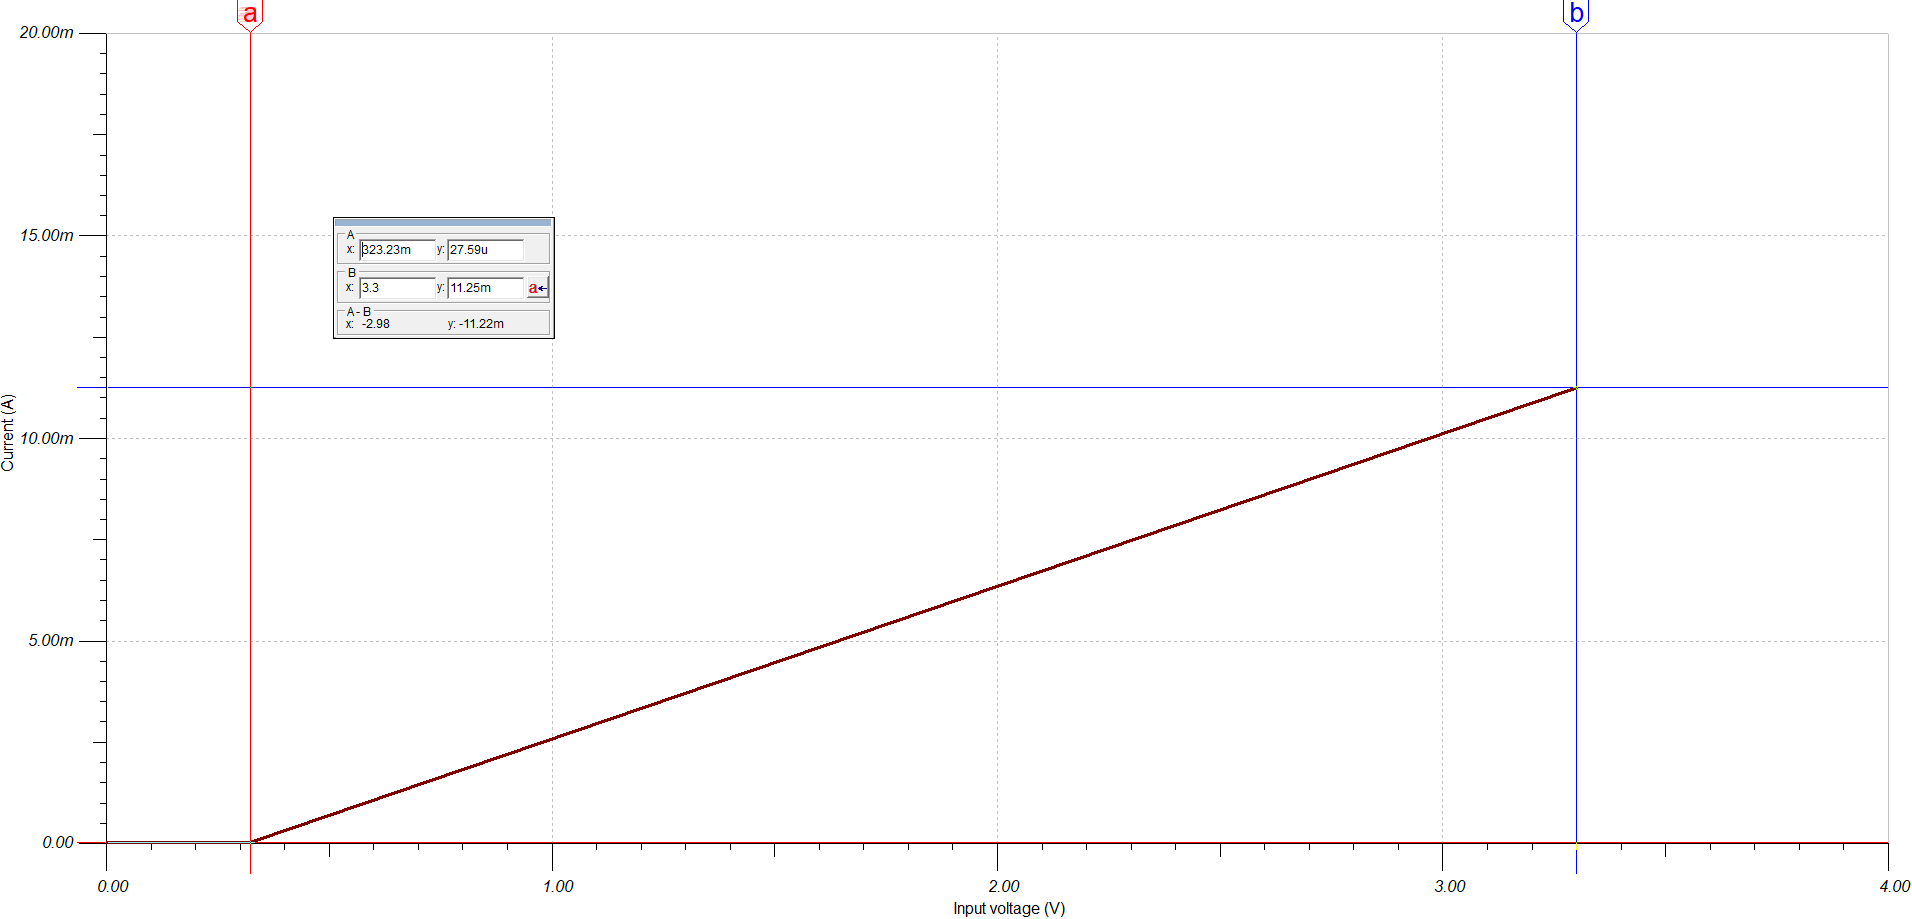
\includegraphics[width=0.9\textwidth]{picture/laser/int-sweep.png}
    \caption{Mô phỏng đặc tuyến V-I trên nguồn internal}
    \label{fig:laser-int-v-i}
\end{figure}

Sử dụng tính năng DC Analysis Table để đo các mức điện áp tại các điểm quan tâm và giá trị dòng thiết kế. So với giá trị dòng điện mong đợi là 12mA, dòng mô phỏng được ở ngõ ra thiết kế là 

\begin{figure}[H]
    \centering
    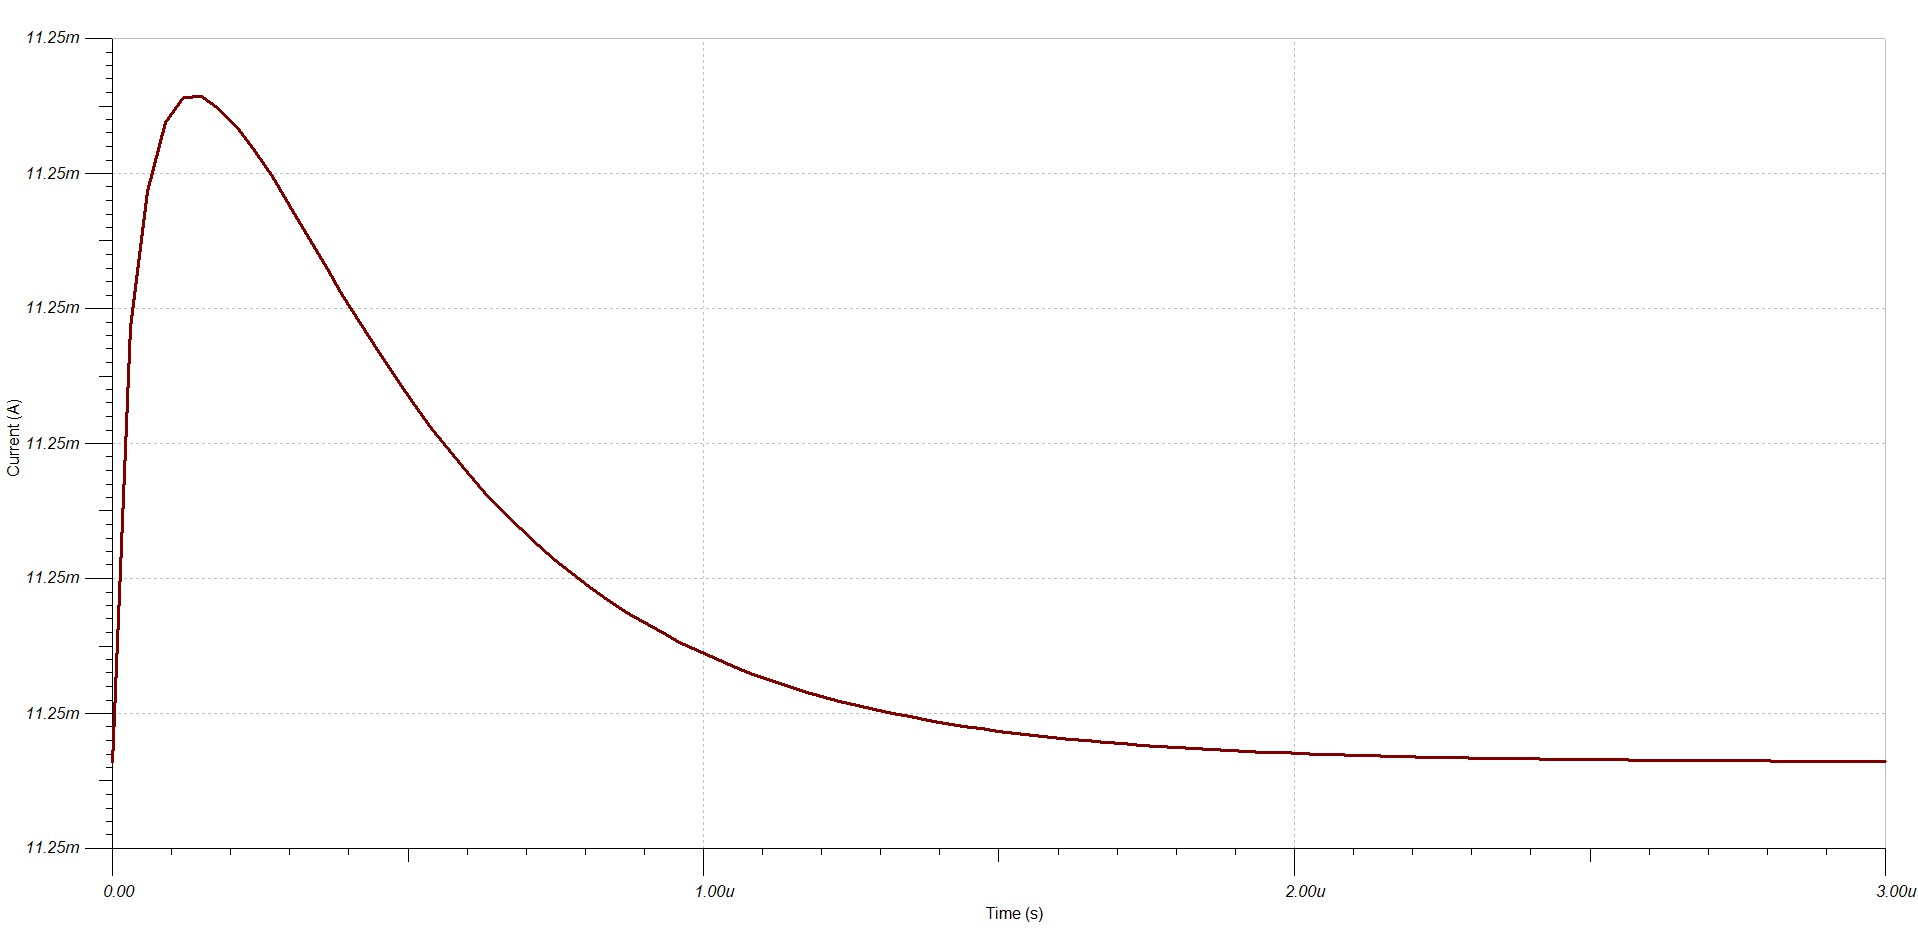
\includegraphics[width=0.9\textwidth]{picture/laser/current-int-transient.jpg}
    \caption{Mô phỏng trạng thái mạch internal ở thời diểm cấp nguồn}
    \label{fig:laser-current-int-transient}
\end{figure}

\begin{figure}[H]
    \centering
    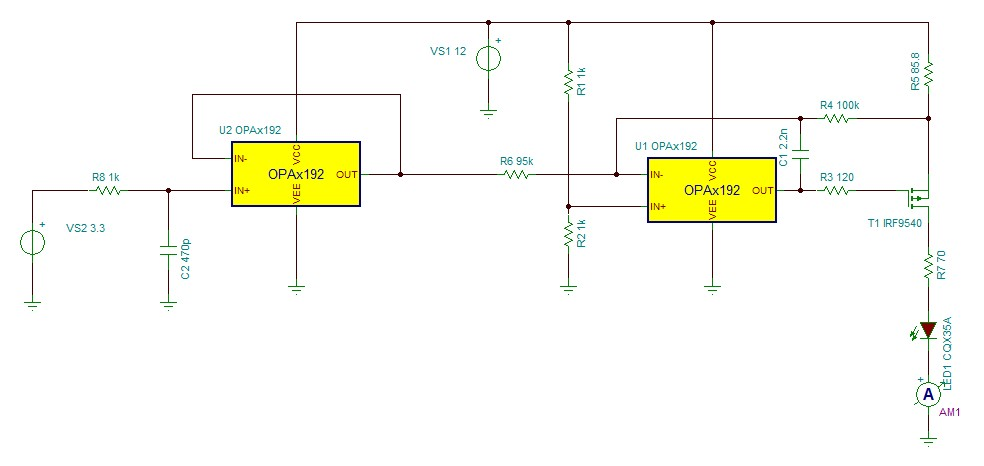
\includegraphics[width=0.9\textwidth]{picture/laser/simulate-current-ext.JPG}
    \caption{Sơ đồ mô phỏng nguồn dòng cho external laser}
    \label{fig:laser-simulate-current-ext}
\end{figure}

\begin{figure}[H]
    \centering
    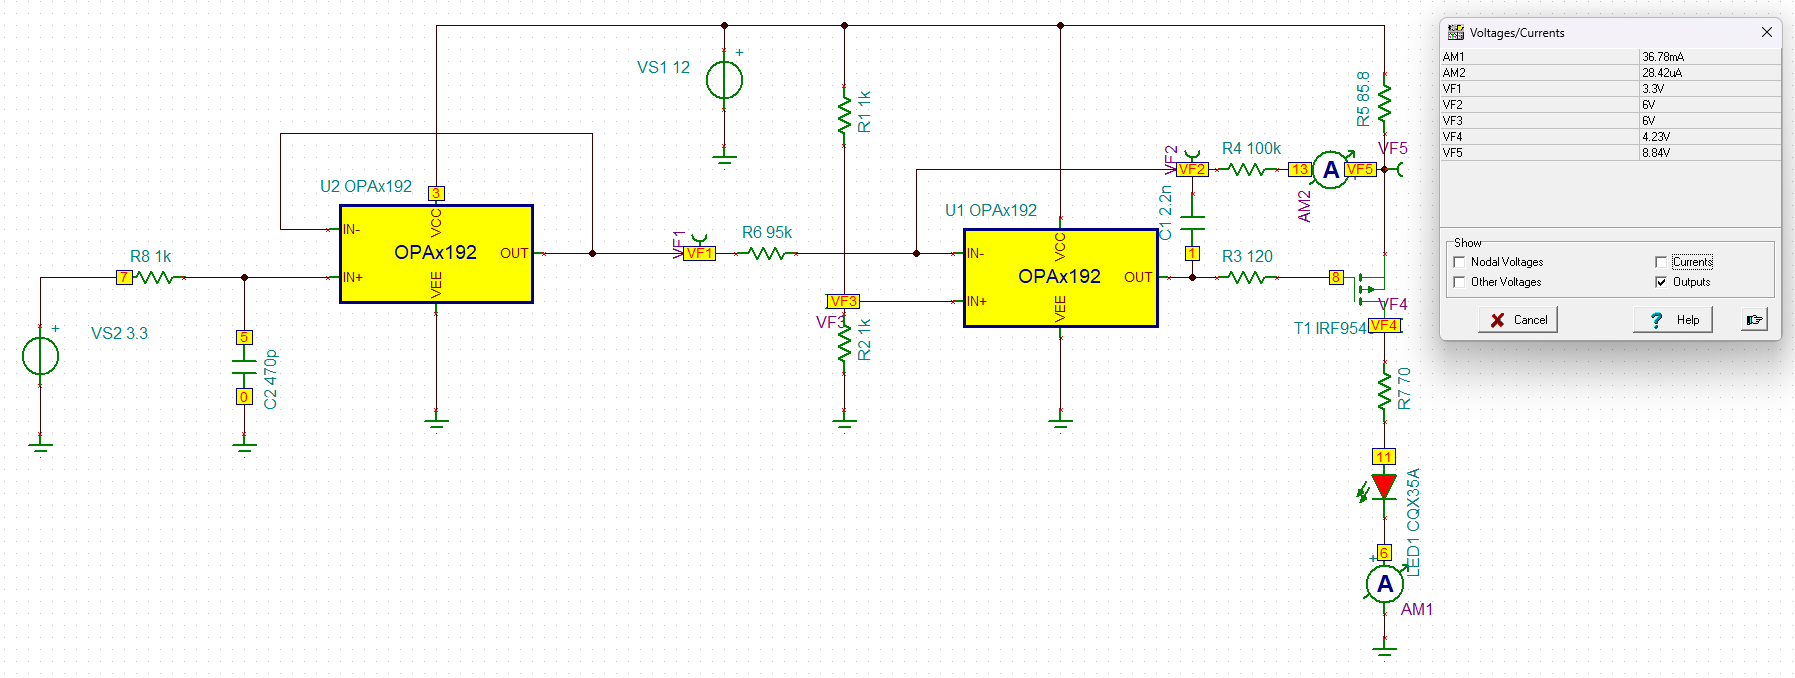
\includegraphics[width=0.9\textwidth]{picture/laser/current-ext-dc-table.png}
    \caption{Bảng giá trị mô phỏng nguồn dòng external}
    \label{fig:laser-current-ext-dc-table}
\end{figure}

\begin{figure}[H]
    \centering
    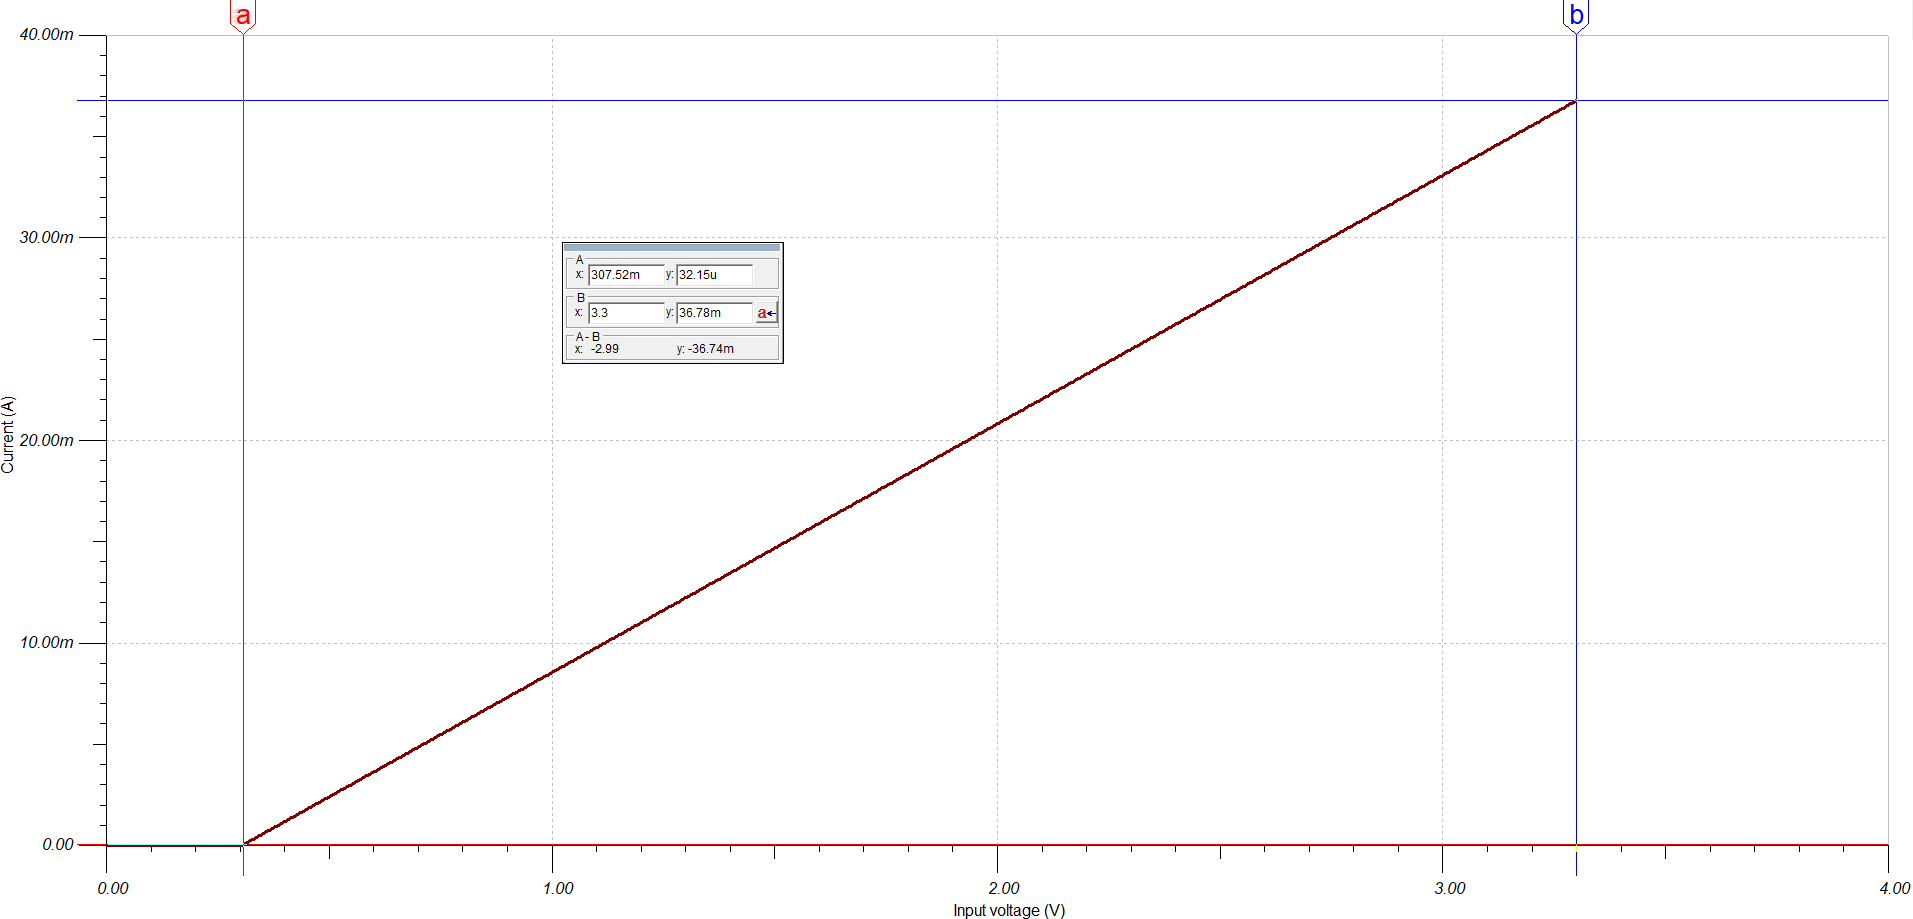
\includegraphics[width=0.9\textwidth]{picture/laser/ext-sweep.png}
    \caption{Mô phỏng đặc tuyến V-I trên nguồn external}
    \label{fig:laser-ext-v-i}
\end{figure}

\begin{figure}[H]
    \centering
    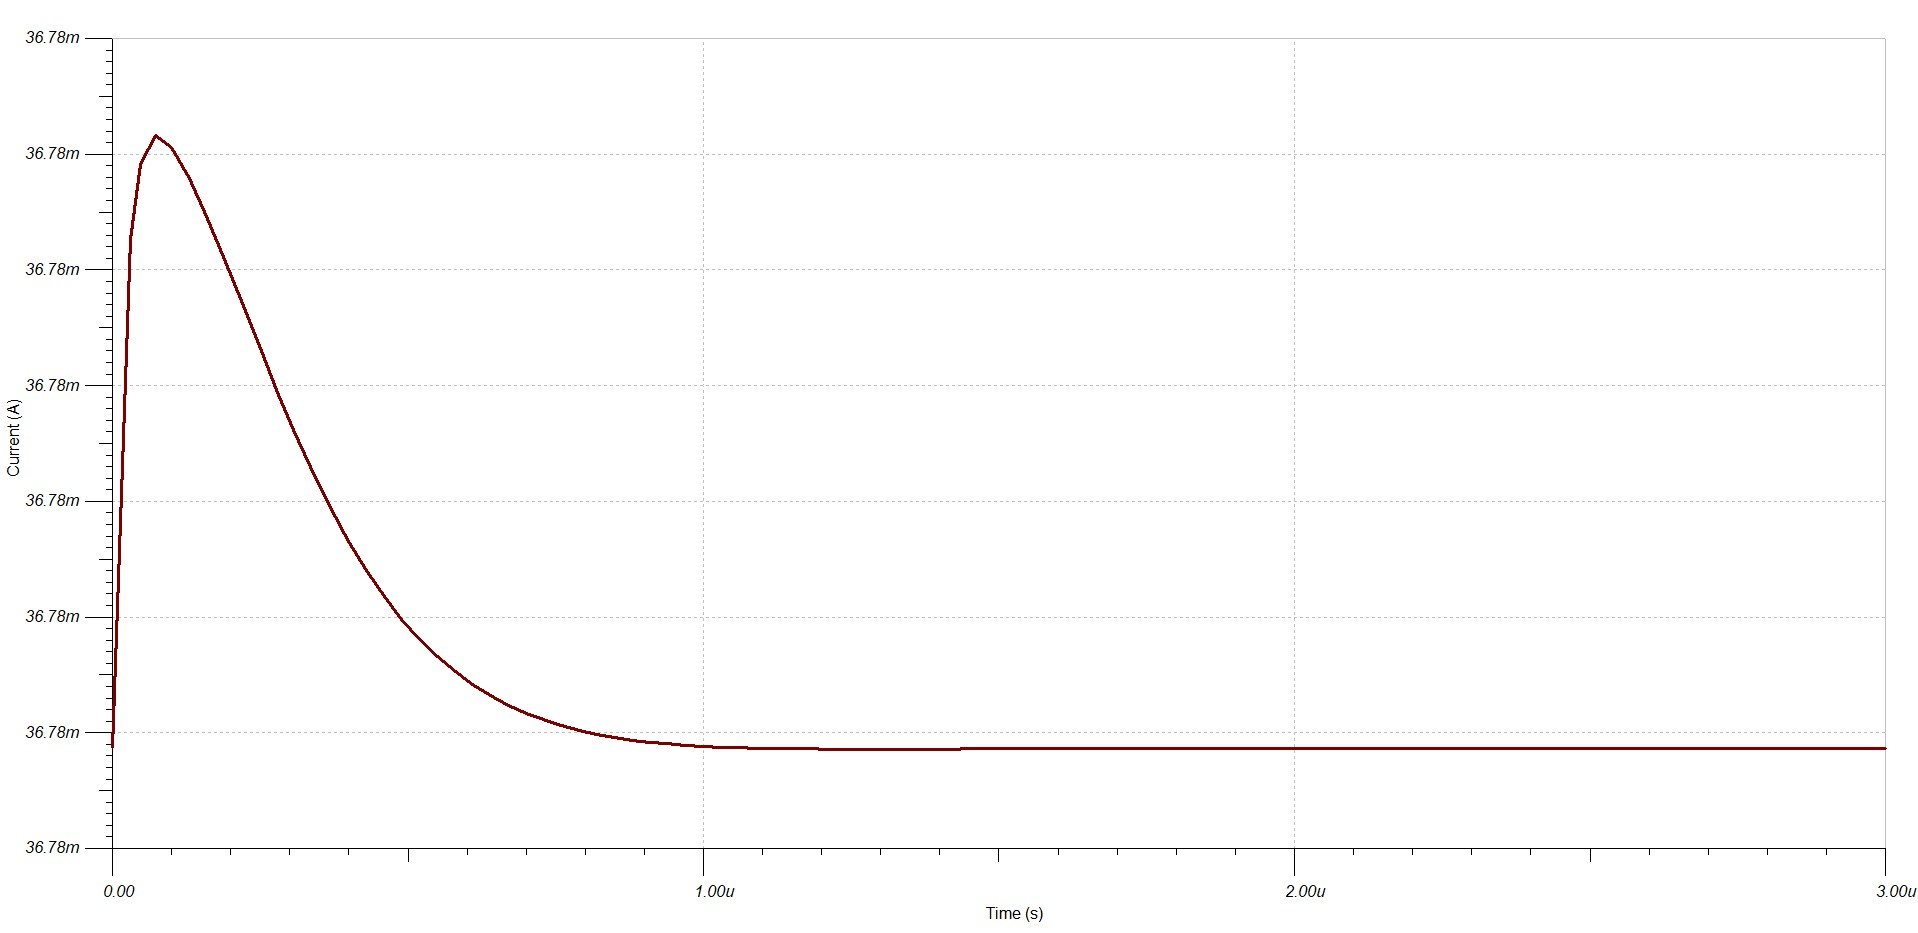
\includegraphics[width=0.9\textwidth]{picture/laser/current-ext-transient.jpg}
    \caption{Mô phỏng trạng thái mạch external ở thời diểm cấp nguồn}
    \label{fig:laser-current-ext-transient}
\end{figure}

\subsubsection{Sơ đồ nguyên lí board LASER DIODE}
\label{so-do-nguyen-li-laser}

\begin{figure}[H]
    \centering
    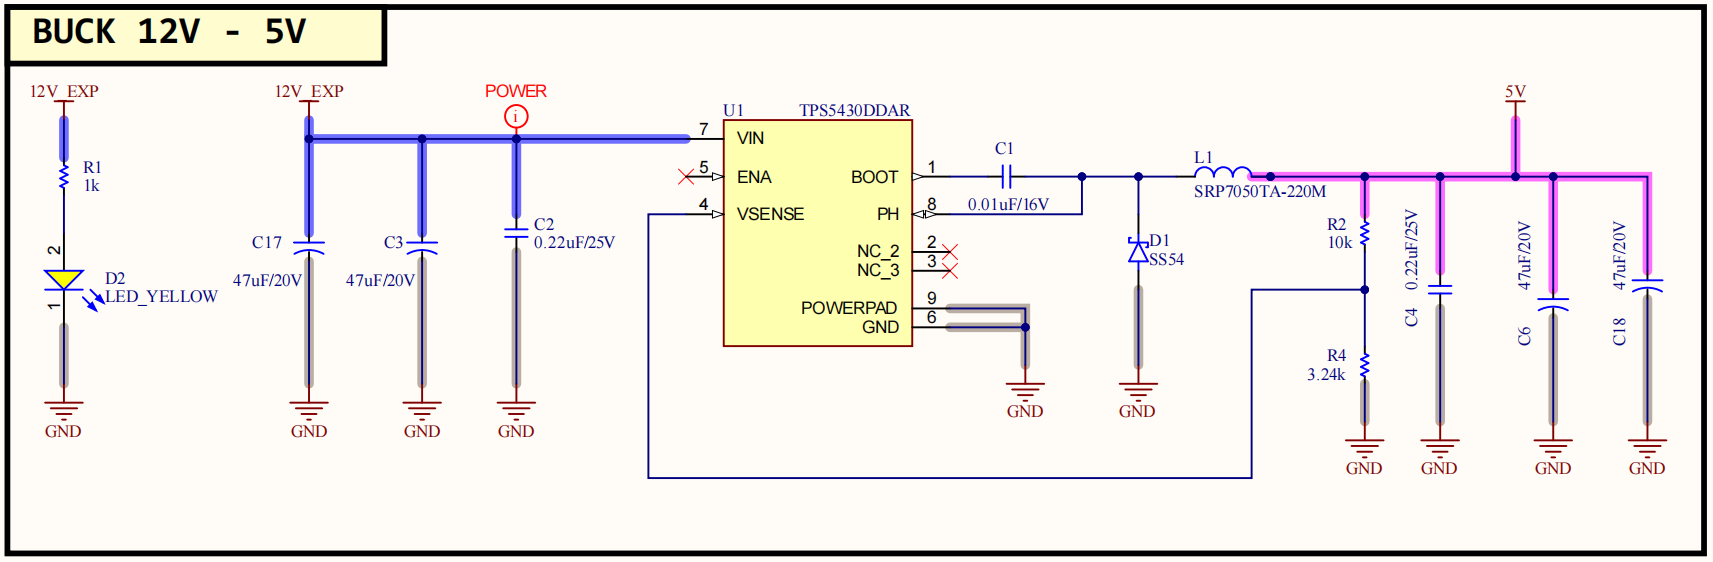
\includegraphics[width=0.9\textwidth]{picture/laser/buck-12-5.png}
    \caption{Mạch nguồn BUCK 12V - 5V }
    \label{fig:laser-buck}
\end{figure}

\begin{figure}[H]
    \centering
    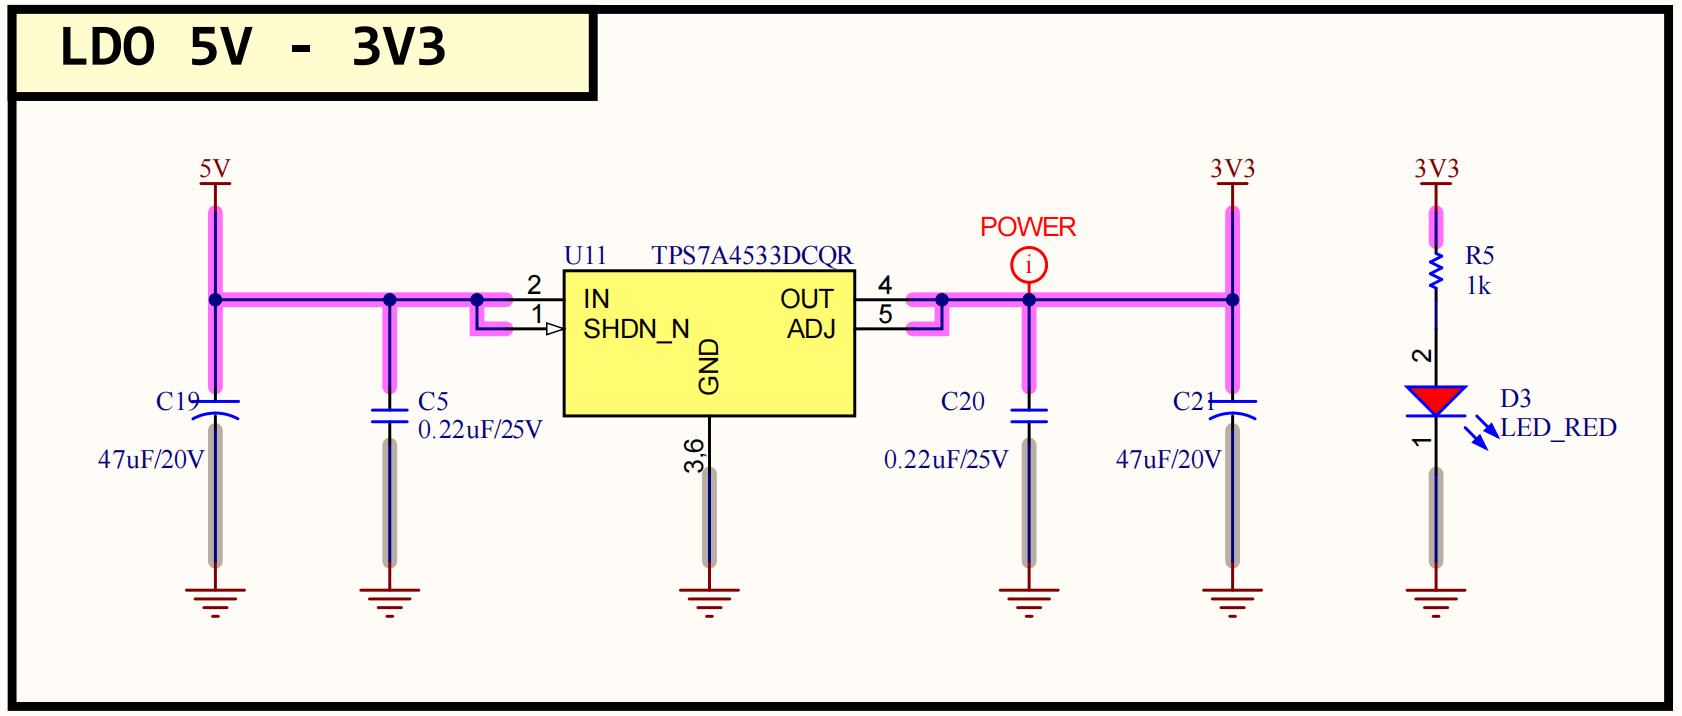
\includegraphics[width=0.9\textwidth]{picture/laser/ldo-5-3v3.png}
    \caption{Mạch nguồn LDO 5V - 3V3}
    \label{fig:laser-ldo}
\end{figure}

\begin{figure}[H]
    \centering
    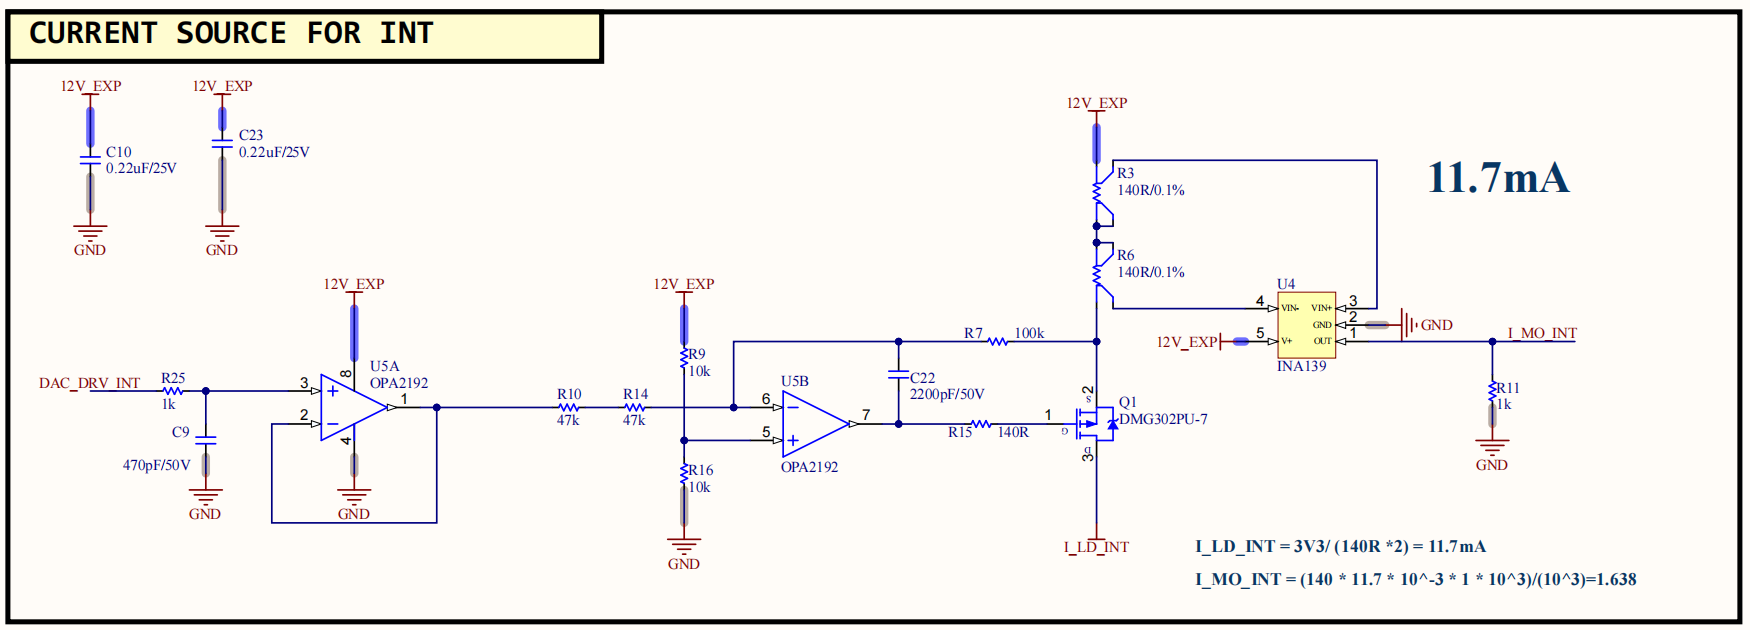
\includegraphics[width=0.9\textwidth]{picture/laser/current-int.png}
    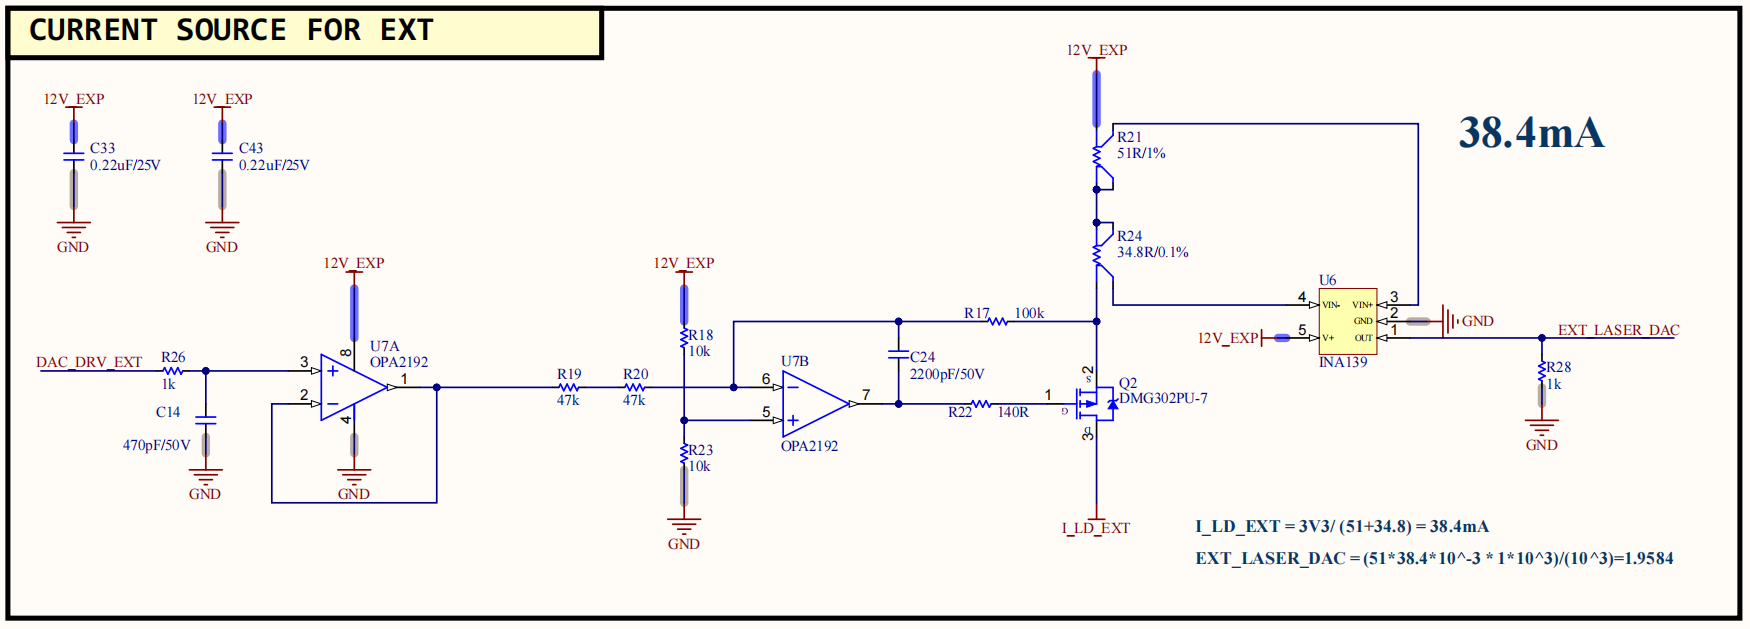
\includegraphics[width=0.9\textwidth]{picture/laser/current-ext.png}
    \caption{Mạch tạo nguồn dòng cho laser diode}
    \label{fig:laser-current}
\end{figure}

\begin{figure}[H]
    \centering
    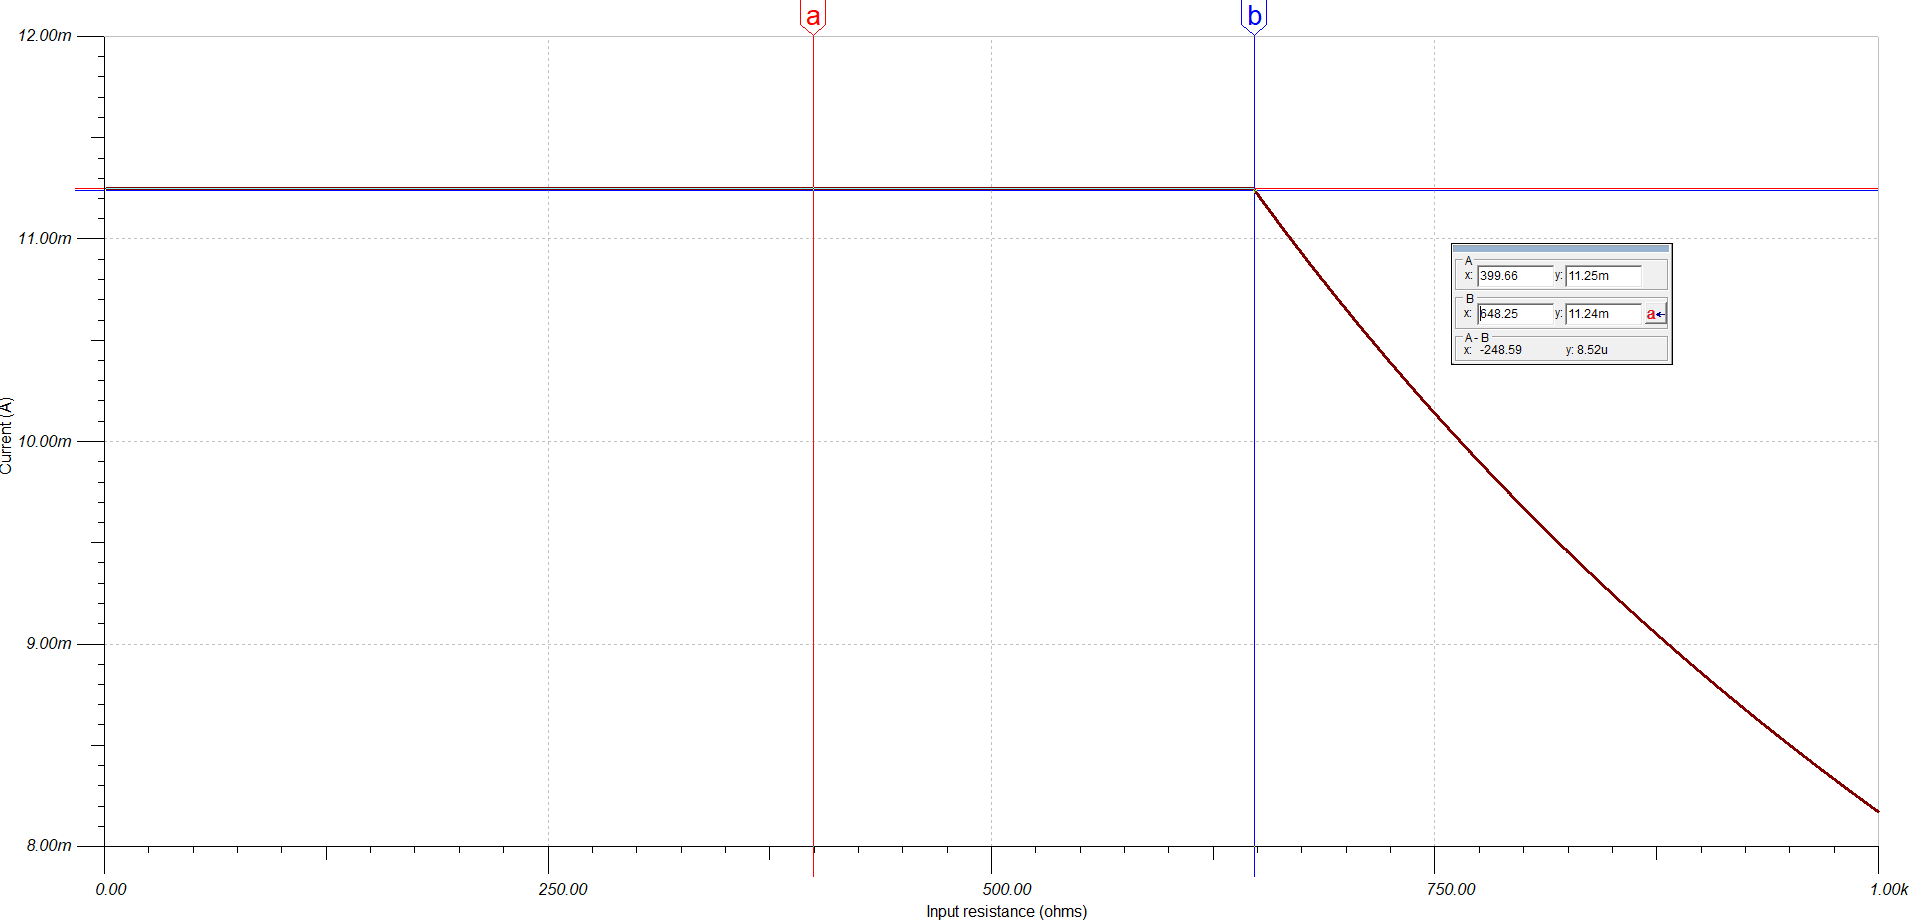
\includegraphics[width=0.9\textwidth]{picture/laser/max-load-int.png}
    \caption{Mạch tải cực đại cho nhánh internal laser}
    \label{fig:laser-max-load-int}
\end{figure}

\begin{figure}[H]
    \centering
    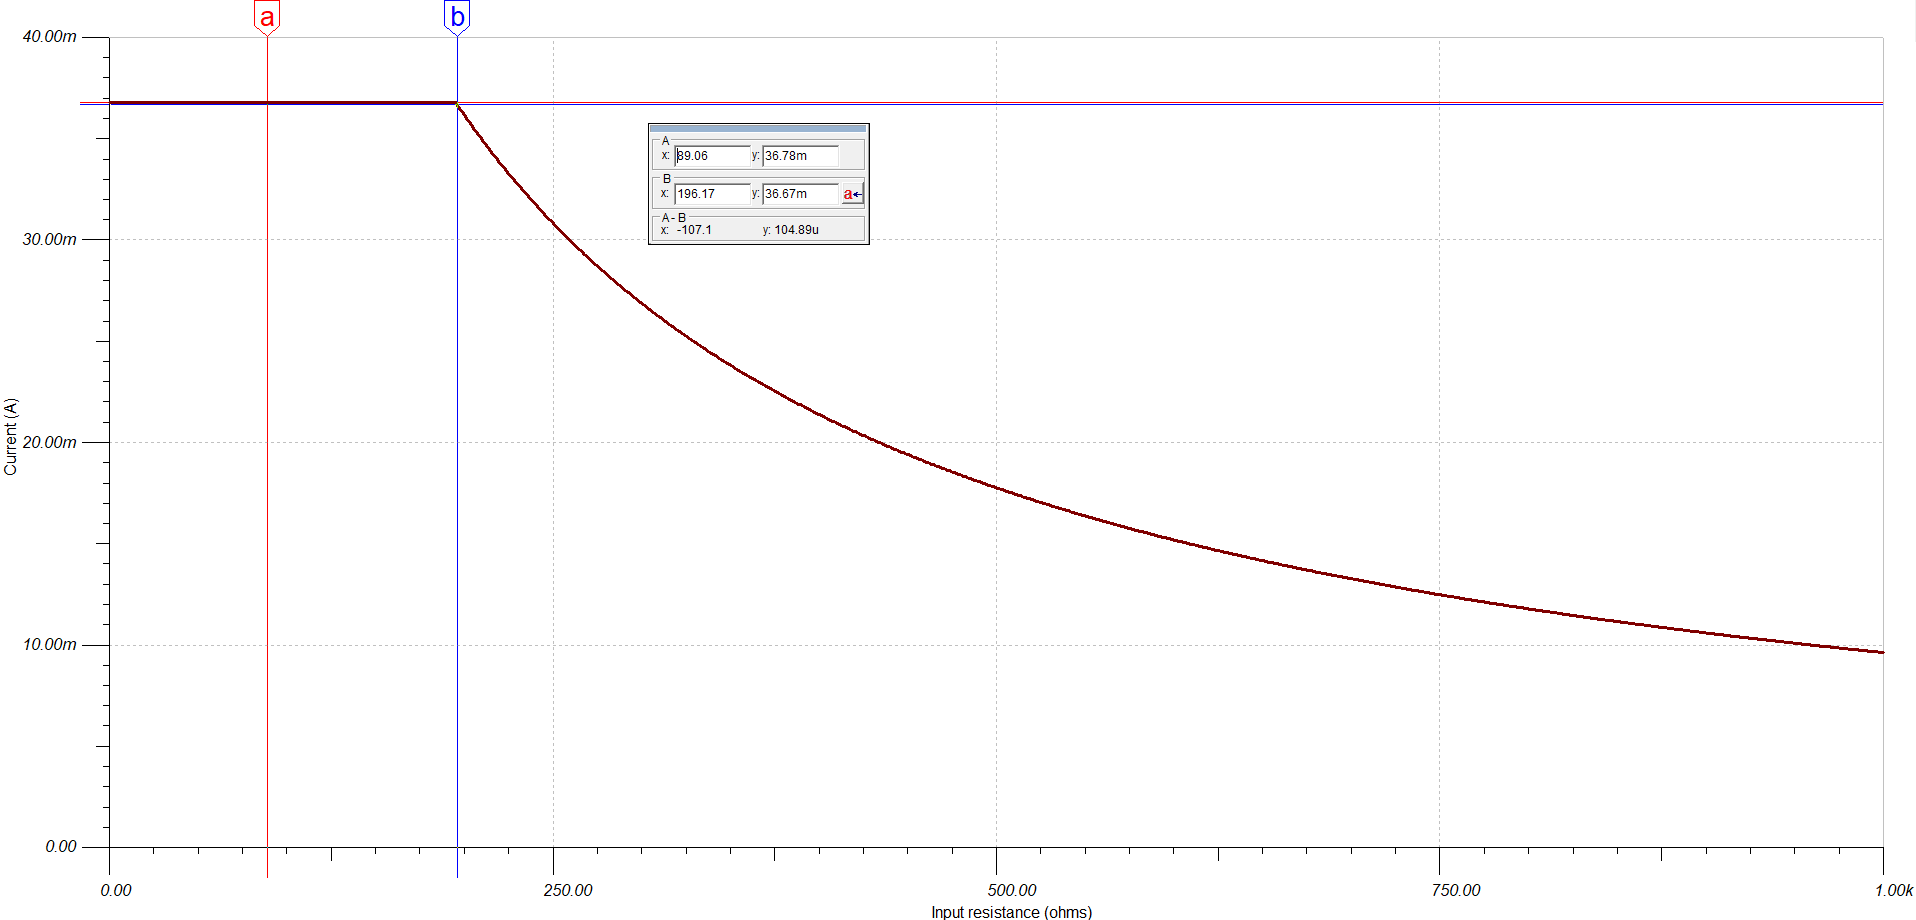
\includegraphics[width=0.9\textwidth]{picture/laser/max-load-ext.png}
    \caption{Mạch tải cực đại cho nhánh external laser}
    \label{fig:laser-max-load-ext}
\end{figure}


\begin{figure}[H]
    \centering
    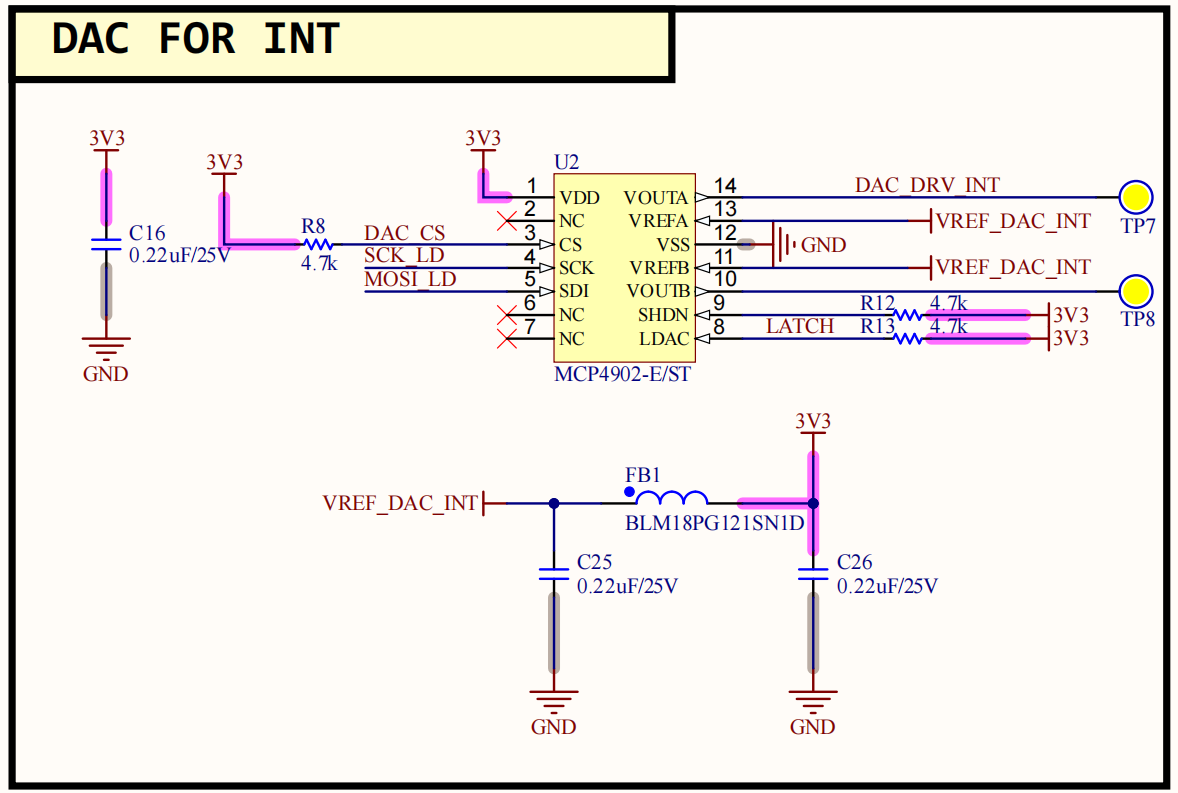
\includegraphics[width=0.8\textwidth]{picture/laser/dac-int.png}
    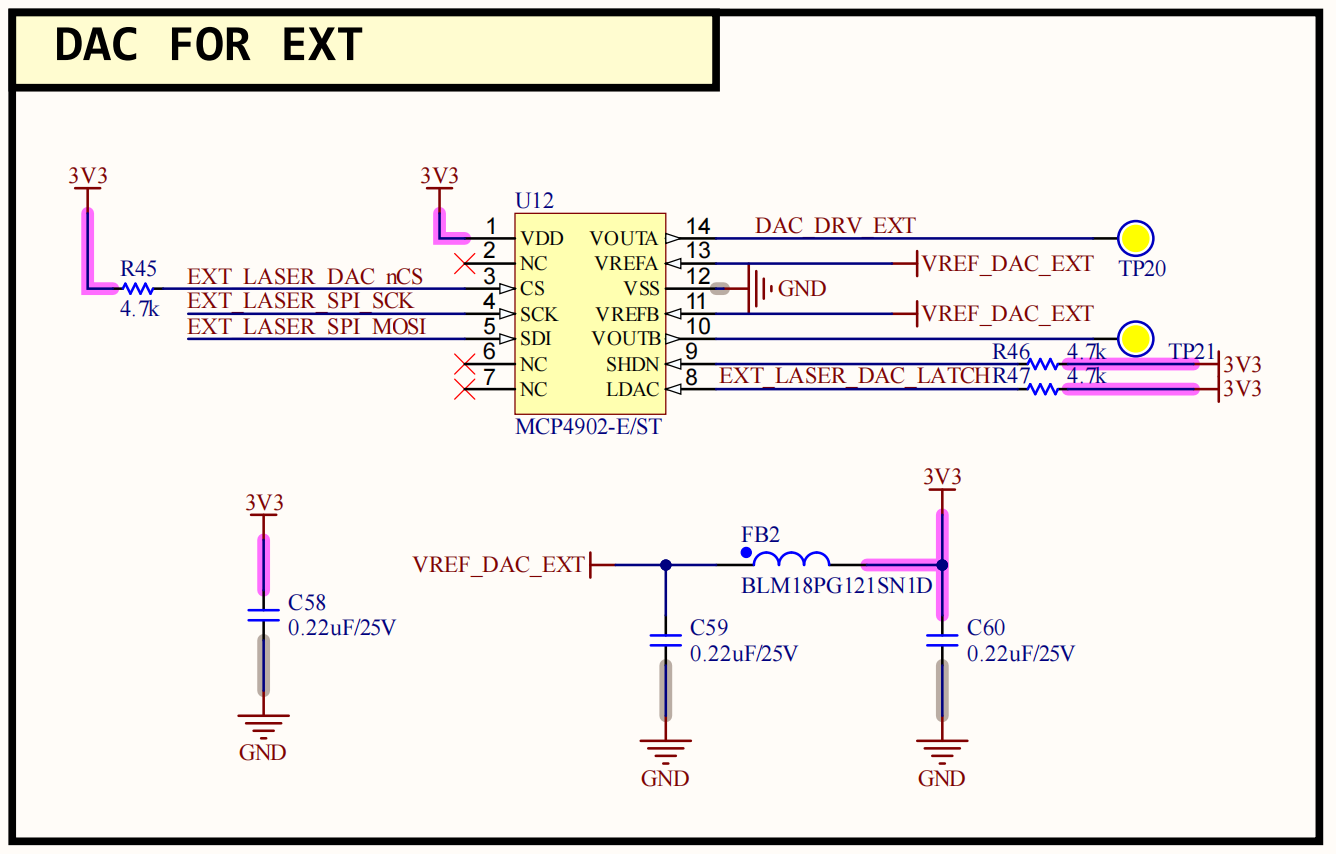
\includegraphics[width=0.8\textwidth]{picture/laser/dac-ext.png}
    \caption{Mạch DAC tạo mức điện áp}
    \label{fig:laser-dac}
\end{figure}

Dòng IC MCP4902/4912/4922 là các bộ chuyển đổi kỹ thuật số sang tương tự (DAC) ngõ ra điện áp kép với độ phân giải lần lượt là 8, 10 và 12-bit, hoạt động từ nguồn đơn 2.7V đến 5.5V. Thiết bị sử dụng kiến trúc chuỗi điện trở (resistive string) kết hợp với các thanh ghi đệm kép để chuyển đổi mã nhị phân thành điện áp tương tự dựa trên điện áp tham chiếu ngoài và hệ số khuếch đại 1x hoặc 2x. Quá trình giao tiếp được thực hiện qua chuẩn SPI (tối đa 20 MHz) với các tín hiệu chính gồm CS (chọn chip), SCK (xung nhịp), SDI (dữ liệu vào), cùng các chân điều khiển LDAC để cập nhật ngõ ra đồng bộ và SHDN để tắt phần cứng. Ưu điểm nổi bật của dòng IC này là thời gian xác lập nhanh (4.5 µs), độ chính xác cao với sai số DNL thấp, hỗ trợ chế độ nhân (Multiplier Mode) và khả năng tiết kiệm điện năng tối ưu thông qua các chế độ tắt linh hoạt trong dải nhiệt độ mở rộng từ -40°C đến +125°C.

\begin{figure}[H]
    \centering
    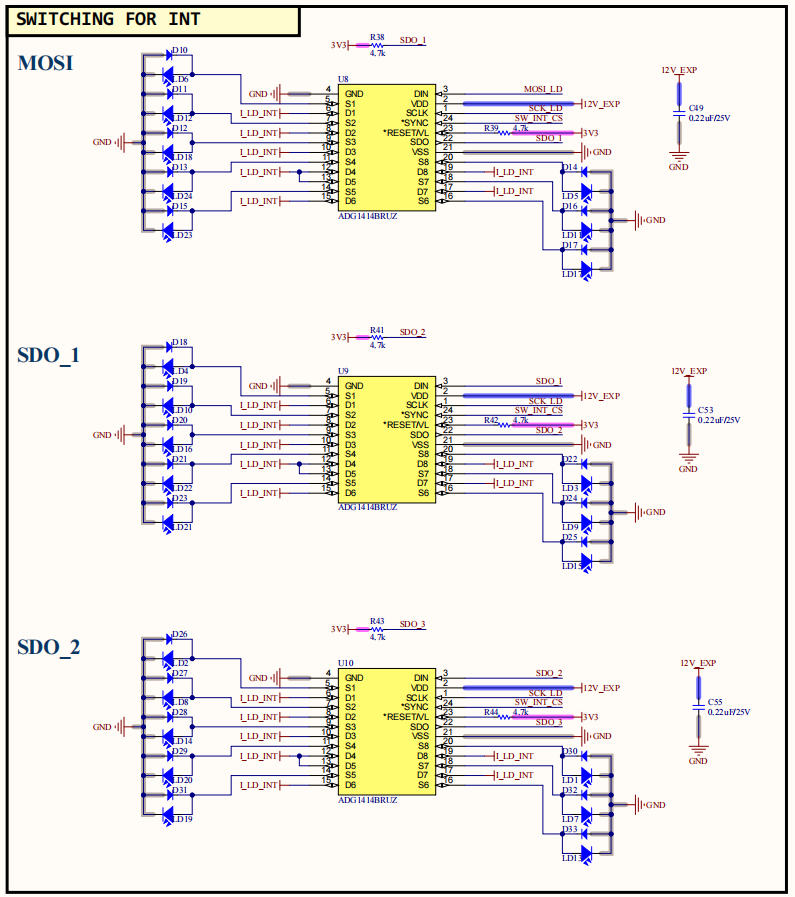
\includegraphics[width=0.9\textwidth]{picture/laser/sw-int.png}
    \caption{Sơ đồ nguyên lí khối LASER - sw-int}
    \label{fig:laser-sw-int}
\end{figure}

\begin{figure}[H]
    \centering
    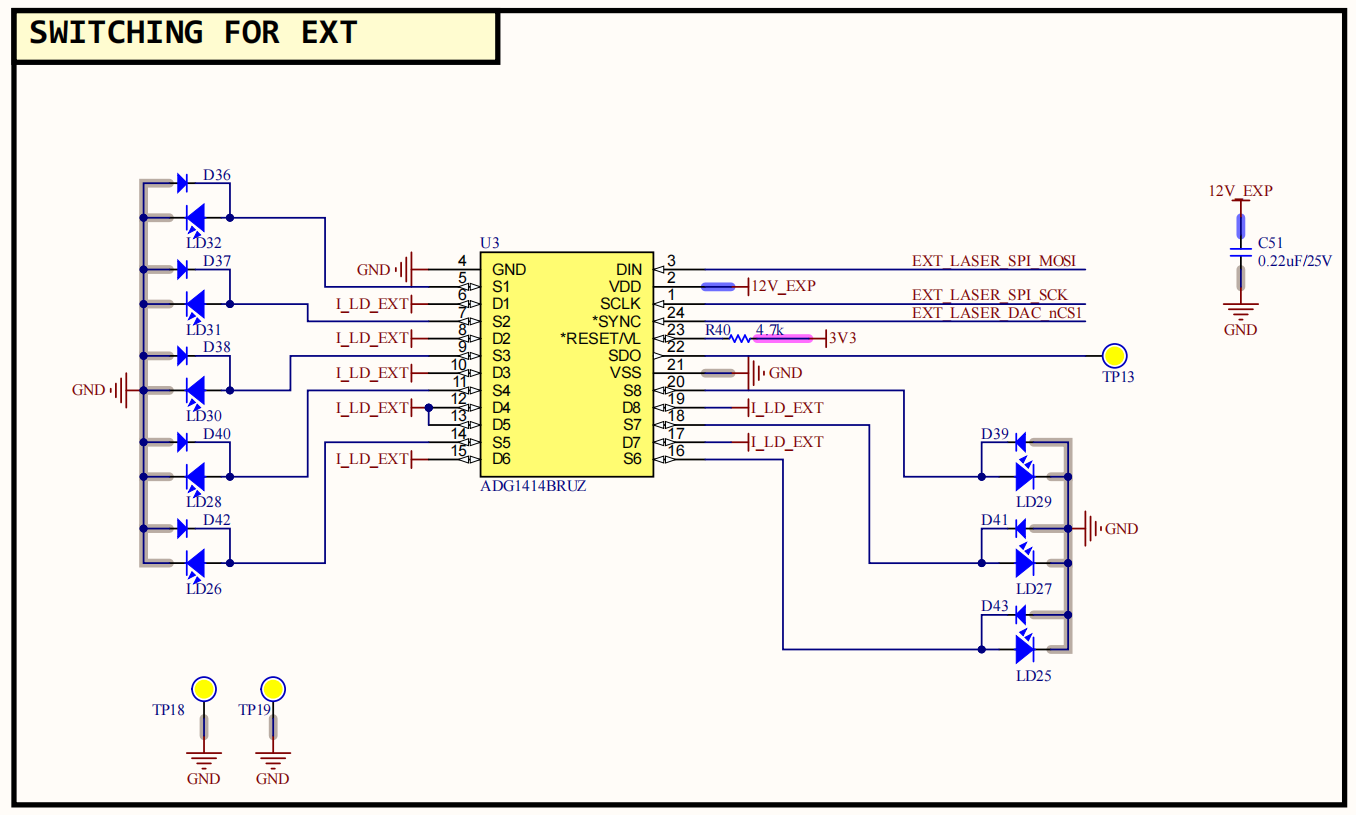
\includegraphics[width=0.9\textwidth]{picture/laser/sw-ext.png}
    \caption{Sơ đồ nguyên lí khối LASER - sw-ext}
    \label{fig:laser-sw-ext}
\end{figure}

ADG1414 là IC tích hợp 8 công tắc SPST điều khiển độc lập. Thiết bị hoạt động bằng cách dịch dữ liệu 8-bit vào thanh ghi nội bộ thông qua giao diện nối tiếp, trong đó mỗi bit tương ứng với trạng thái đóng hoặc ngắt của một kênh công tắc. IC này hỗ trợ khả năng mắc nối tiếp (daisy-chain) nhiều thiết bị với nhau thông qua chân SDO (Serial Data Output). Trong cấu hình này, chân SDO của thiết bị phía trước được kết nối với chân DIN của thiết bị tiếp theo. Khi nạp nhiều hơn 8 bit dữ liệu vào chuỗi, các bit dữ liệu sẽ lần lượt được đẩy ra khỏi thanh ghi dịch qua chân SDO để truyền sang thiết bị kế tiếp. Tổng số xung nhịp cần thiết để cấu hình toàn bộ chuỗi là 8 × N (với N là số lượng IC trong chuỗi). Chân SDO là dạng cực máng hở (open-drain), vì vậy cần sử dụng một điện trở kéo lên nguồn VL khi kết nối. Các tín hiệu giao tiếp chính bao gồm SYNC (đồng bộ khung), SCLK (xung nhịp tối đa 50 MHz) và DIN (dữ liệu vào), tương thích với các chuẩn SPI, QSPI và MICROWIRE. Ưu điểm của IC bao gồm điện trở dẫn (RON) là 9.5 Ω, độ phẳng điện trở là 1.6 Ω và khả năng dẫn tín hiệu rail-to-rail trên dải nguồn cấp rộng như ±15 V, +12 V hoặc ±5 V.




% \subsection{Board thu năng lượng ánh sáng - PHOTO}
% \label{subsec:sche-board-thu-photo}

\newpage













